% arara: pdflatex: { synctex: on } 
% arara: makeindex 
% arara: pdflatex: { synctex: on } 

\newcommand{\version}{0.95}


%todo
% language/logic/mapping registration process - maybe in a different document

% more useful EBNF (see CASL RefMan)

% This file was initially converted to LaTeX by Writer2LaTeX ver. 1.1.8
% (see http://writer2latex.sourceforge.net for more info)
% 
% Further formatting was done using the isov2 LaTeX package

%% Global switches
% Do we pretend that this is a final version?
\newif\ifpretendfinal
\pretendfinaltrue 

% Real PDF comments, or "paper" margin notes (using todonotes package)?
\newif\ifpdfcomment
%\pdfcommenttrue
\pdfcommentfalse

\documentclass[10pt,fleqn,%
\ifpretendfinal
final%
\else
draft%
\fi,
%final,
]{scrreprt}

\usepackage{pdflscape}

%\usepackage[show]{ed}
\usepackage[hide]{ed}

%color highlight, for editing
\usepackage{color}
\newcommand{\red}[1]{#1} %{\color{red}{#1}}} % currently, no color highlighting


%% Hacks
%\usepackage{savesym}

%\usepackge{enumitem}

%% Font and language
\usepackage[utf8]{inputenc}
\usepackage[T1]{fontenc}
\usepackage[english]{babel}
\usepackage{textcomp}
%\usepackage{lmodern} % FN: commented out since OMG wants its own fonts
%\usepackage[scaled=.8]{beramono} % FN: commented out since OMG wants its own fonts
\usepackage{courier}
\usepackage[scaled=.9]{helvet}

% set up Unicode symbols
\DeclareUnicodeCharacter{21A6}{\ensuremath{\mapsto}}


% Keyword Index 
\usepackage{makeidx}
\makeindex
% used in definition of \termref, \termdefinition  

\newcommand{\dolindex}{Distributed Ontology Modeling and Specification Language (DOL)}

%% Math
% \usepackage{mathtools}
% reintroducing a math-style \begin{definition}…\end{definition} environment
% \usepackage{amsthm}
% \theoremstyle{definition}
% \newtheorem{definition}{Definition}
\usepackage{hetonto-subset}
% \usepackage{diagrams}

%% Utilities
\usepackage{etoolbox}
\usepackage{ifmtarg}
\usepackage{stringstrings}
\usepackage{stmaryrd}
\usepackage{enumitem}

%% Graphics
\usepackage{standalone}
\usepackage[final]{graphicx}
\usepackage{tikz}
\usepackage{rotating}
\usetikzlibrary{matrix,shapes,arrows,calc}
\usepackage{tikz-uml}
\usetikzlibrary{shadows,shapes,positioning,arrows}
\tikzstyle{ontoiop}=[font=\sffamily,
    language/.style={circle,draw},
    translation/.style={-stealth'},
    dol/.style={rectangle,rounded corners,draw,align=left},
    import/.style={-o},
]
% Our colors
\definecolor{cl}{RGB}{127,129,209}
\definecolor{owl}{RGB}{138,173,72}
\definecolor{rdfs}{RGB}{232,146,31}
\definecolor{dol}{RGB}{253,246,234}
\definecolor{owlxml}{RGB}{240,251,239}
\definecolor{clif}{RGB}{242,242,251}


%% Content
\usepackage{ctable}
\usepackage[final]{listings}
\lstset{basicstyle=\ttfamily\small,columns=fixed}
\usepackage{lstsemantic}
\usepackage{algorithmic}

%% linguistics
\usepackage{xspace}
% English
\newcommand*{\cf}{cf.\@\xspace}
\newcommand*{\eg}{e.g.\@\xspace}
\newcommand*{\etal}{et al.\@\xspace}
\newcommand*{\ie}{i.e.\@\xspace}
\newcommand*{\vs}{vs.\@\xspace}
\newcommand*{\wrt}{w.r.t.\@\xspace}
% Quotes
\usepackage[babel]{csquotes} 
\MakeAutoQuote{“}{”}
\MakeAutoQuote*{‘}{’}
% FN: can we remove that? the quotation marks lead to errors in my editor, so I removed them in the source code anyway. 

%% Hyperref
\usepackage[
          % we want hyperlinks even in draft mode
          final,
          plainpages=false,
          pdfpagelabels,
          bookmarksnumbered,
          hyperindex=true
         ]{hyperref}

%% To-do notes and/or comments
% \savesymbol{todo}
% \restoresymbol{ed}{todo}

\usepackage{xkeyval}
\makeatletter
% author
\newcommand*\CommentAuthor{}
\define@key{Comment}{author}{%
\renewcommand*\CommentAuthor{#1}}
% date
\newcommand*\CommentDate{}
\define@key{Comment}{date}{%
\renewcommand*\CommentDate{#1}}
% id
\newcommand*\CommentId{}
\define@key{Comment}{id}{%
\renewcommand*\CommentId{#1}}
% replyto
\newcommand*\CommentReplyTo{}
\define@key{Comment}{replyto}{%
\renewcommand*\CommentReplyTo{#1}}
% type (currently represented as color and text prefix)
\newcommand*\CommentType{}
\define@key{Comment}{type}{%
\renewcommand*\CommentType{#1}}
\makeatother
\presetkeys{Comment}{%
author=,date=,id=,replyto=,type=}{}%

\newcommand*{\SetCommentColorByType}[1]{%
% http://tex.stackexchange.com/questions/24922/comparing-an-argument-to-a-string-when-argument-is-a-result-of-a-command-with-et
\edef\localType{{#1}}% enforce expansion of #1
\expandafter\ifstrequal\localType{q-aut}{\colorlet{CommentColor}{red}}{%
\expandafter\ifstrequal\localType{q-all}{\colorlet{CommentColor}{orange}}{%
\expandafter\ifstrequal\localType{todo}{\colorlet{CommentColor}{orange}}{%
\expandafter\ifstrequal\localType{fyi}{\colorlet{CommentColor}{lightgray}}{%
\colorlet{CommentColor}{yellow}}}}}}
\makeatletter
\newcommand*{\SetCommentPrefixByType}[1]{%
\edef\localType{{#1}}% enforce expansion of #1
\expandafter\@ifmtarg\localType{% if empty
\edef\CommentPrefix{}%
}{% if not empty
\caseupper[q]{#1}%
\edef\CommentPrefix{\thestring: }%
}}
\makeatother

\newcommand*{\initComment}[1]{%
\setkeys{Comment}{#1}%
\SetCommentColorByType{\CommentType}%
\relax%
\SetCommentPrefixByType{\CommentType}%
\relax%
}

\makeatletter
\ifpdfcomment
% forward class options "draft" or "final" into document
\ifdr@ftd@c
\usepackage[draft]{pdfcomment}
\else
\usepackage[final]{pdfcomment}
\fi

\newcommand*{\todonote}[2][]{%
\initComment{#1}%
\pdfcomment[author=\CommentAuthor,color=CommentColor,date=\CommentDate,id=\CommentId]{%
\CommentPrefix
%\usebox{CommentPrefix}
#2}}


\newcommand*{\reply}[2][]{%
\initComment{#1}%
\pdfreply[author=\CommentAuthor,color=CommentColor,date=\CommentDate,id=\CommentId,replyto=\CommentReplyTo]{%
%\usebox{CommentPrefix}
#2}}

\newcommand*{\markupcomment}[3][]{%
\initComment{#1}%
\pdfmarkupcomment[author=\CommentAuthor,color=CommentColor,date=\CommentDate,id=\CommentId]{#2}{%
%\usebox{CommentPrefix}
#3}}

% Hyperlinks don't work inside pdfcomment's PDF comments :-(
\newcommand*{\todonoteURL}[1]{#1}
%\else % \ifpdfcomment
%\ifdr@ftd@c
%\usepackage[show]{ed}
%\else
%\usepackage[hide]{ed}
%\fi
% \usepackage[obeyDraft,textsize=tiny]{todonotes} % must load after tikz

%FN I commented the above out, because I could not get it to work, instead I include
 



\renewcommand*{\todonote}[2][]{% FN: Changed newcommand to renewcommand
\initComment{#1}%
% TODO set color according to type
% TODO display author (unless empty)
% TODO display date (unless empty)
\ednote{\CommentPrefix #2}}

\renewcommand*{\reply}[2][]{% FN: Changed newcommand to renewcommand
\initComment{#1}%
% TODO set color according to type
% TODO display author (unless empty)
% TODO display date (unless empty)
\ednote{Reply: \CommentPrefix #2}}

\renewcommand*{\markupcomment}[3][]{% FN: Changed newcommand to renewcommand
\initComment{#1}%
% TODO set color according to type
% TODO display author (unless empty)
% TODO display date (unless empty)
\ednote{\CommentPrefix #3}#2}

% dummy versions of some pdfcomment commands
\renewcommand*{\textLF}{\\}

\renewcommand*{\todonoteURL}[1]{\url{#1}}
%\fi % \ifpdfcomment FN: commented this out
\makeatother
\newcommand*{\ticket}[1]{\todonoteURL{http://trac.informatik.uni-bremen.de:8080/OntoIOp/ticket/#1}}

% comment commands for frequent users
\newcommand*{\CLnote}[2][author=Christoph Lange]{%
\todonote[author=Christoph Lange,#1]{#2} 
}




%% ISO structures not defined by isov2.cls, and additional semantic macros
% cross-reference to a normative reference
\newcommand*{\nitem}[1]{[#1]}
% reference from the definition of one term to another defined term
\newcommand*{\termref}[1]{\index{#1}#1\xspace}
% subject field restriction of a term
\newcommand*{\subjectfield}[1]{ {\textlangle}#1{\textrangle}}
% synonym of a term
\newcommand*{\synonym}{; }
% MIME type
\newcommand*{\mimetype}[1]{\textit{#1}}
% Font style for syntactic features only supported with institutions
\newcommand*{\institutionsOnly}{\bfseries\itshape}
% Font style for syntactic features
\newcommand*{\syntax}[1]{\texttt{#1}}


% requirements (as per Annex H of ISO/IEC Directives, Part 2)
\newcommand*{\notallowed}{\textbf{not allowed}\xspace}
\newcommand*{\notrequired}{\textbf{not required}\xspace}
\newcommand*{\required}{\textbf{required}\xspace}
\newcommand*{\recommended}{\textbf{recommended}\xspace}
\newcommand*{\shallnot}{\textbf{shall not}\xspace}
\newcommand*{\shall}{\textbf{shall}\xspace}
\newcommand*{\shouldnot}{\textbf{should not}\xspace}
\newcommand*{\should}{\textbf{should}\xspace}
\newcommand*{\may}{\textbf{may}\xspace}
\newcommand*{\hasto}{\textbf{has to}\xspace}

% abbreviations
\newcommand*{\IS}{OMG Specification\xspace}

%% Math macros
%\newcommand{\Mod}{\ensuremath{\mathrm{Mod}}}
%\newcommand{\Sen}{\ensuremath{\mathrm{Sen}}}
%\newcommand{\Sign}{\ensuremath{\mathrm{Sign}}}
\newcommand{\conjclause}{\ensuremath{p_1 \wedge \dots \wedge p_n}}
\newcommand{\id}{\ensuremath{\operatorname{id}}}
\newcommand{\powerset}[1]{\mathcal{P}(#1)}
\newcommand{\finorderedpowerset}{\mathcal{P}^{\mathrm{ord}}_{\mathrm{fin}}}
\newcommand{\finpowerset}{\mathcal{P}_{\mathrm{fin}}}
\newcommand{\reductop}{\mathnormal{|}}

%% from HetCASL summary
\newcommand{\Si}{\Sigma}
\newcommand{\al}{\alpha}
%\newcommand{\sen}{\mathbf {Sen}}
\newcommand{\ModFunctor}{\mathbf{Mod}}
\newcommand{\SenFunctor}{\mathbf{Sen}}
\newcommand{\Sig}{\mathsf{Sig}}
\renewcommand{\Th}{\mathsf{Th}}
\newcommand{\Mor}{\mathsf{Mor}}
\newcommand{\PF}{\mathit{PF}}
\newcommand{\TF}{\mathit{TF}}

\newcommand{\Inst}{\ensuremath{\mathbf{Inst}}}
\newcommand{\Name}{\ensuremath{\mathbf{Name}}}

%\newcommand{\map}[2]{\colon#1\!\longrightarrow\!#2}

\newcommand{\Gram}[1]{\texttt{#1}}
\newcommand{\Gx}[1]{\texttt{#1}}

\newenvironment{Grammar}
 {%\texonly{\footnotesize}
  \begin{example}}{\end{example}\ignorespaces}

\newenvironment{AbstractGrammar}
 {\par%\texonly{\smallskip\samepage}
   \begin{Grammar}}{\end{Grammar}\par}

\newenvironment{ConcreteDisplay}
 {\nopagebreak\begin{quote}\casl}{\end{quote}\pagebreak[3]}

\newenvironment{ConcreteInput}
 {\begin{example}}{\end{example}\ignorespaces}

\newcommand{\DisplayLatexInput}[3]
 {The sign displayed as 
 \texorhtml{`\begin{casl}\(#1\)\end{casl}'}{#2 in \LaTeX}
 is input as `\Gram{#3}'.} 

\newcommand{\DisplayISOInput}[3]
 {The sign displayed as `\begin{casl}\(#1\)\end{casl}' may be input as
 `\math{#2}' in ISO Latin-1, or as `\Gram{#3}' in ASCII.} 

\newcommand*{\CL}{\ensuremath{\mathsf{CL}}\xspace}
\newcommand{\QL}{\ensuremath{\mathsf{QL}}\xspace}
\newcommand{\RL}{\ensuremath{\mathsf{RL}}\xspace}
\newcommand{\EL}{\ensuremath{\mathsf{EL}}\xspace}

\newcommand*{\meta}{\ensuremath{\operatorname{meta}}\xspace}

\newcommand{\BASICOMS}{\ensuremath{\langle\Sigma,\Delta\rangle}\xspace}

\newcommand{\semdom}[1]{
\begin{center}
\fbox{$#1$}
\end{center}
}

\newcommand{\mBox}[1]{\, \mbox{#1} \,}
\newcommand{\twocase}[3]{
\left\{
\begin{array}{ll}
  #1,&\mBox{if }#2\\
  #3,&\mBox{otherwise}
\end{array}\right.}

\newcommand{\threecase}[5]{
\left\{
\begin{array}{ll}
  #1,&\mBox{if }#2\\
  #3,&\mBox{if }#4\\
  #5,&\mBox{otherwise}
\end{array}\right.}





% Logics
\newcommand{\ELDL}{\ensuremath{\mathcal{EL}}\xspace}
\newcommand*{\DOL}{\ensuremath{\mathsf{DOL}}\xspace}
\newcommand*{\PL}{\ensuremath{\mathit{PL}}\xspace}
\newcommand{\CLminus}{\CL$^-$} 

% translations
\newcommand{\translate}[2]{\ensuremath{{#1}{\to}{#2}}\xspace}
\newcommand{\PropToOWL}{\translate\Prop\OWL}
\newcommand{\PropToFOL}{\translate\Prop\FOL}
\newcommand{\ELToOWL}{\translate\EL\OWL}
\newcommand{\OWLToFOL}{\translate\OWL\FOL}
\newcommand{\OWLToCL}{\translate\OWL\CL}
\newcommand{\FOLToCL}{\translate\FOL\CL}

%% Common Logic


\newcommand{\holds}[1]{\ensuremath\mathtt{Holds}_{#1}\xspace}
\newcommand{\apply}[1]{\ensuremath\mathtt{App}_{#1}\xspace}


% FN: Latex Hacks by Fabian 

% Sourcecode from isov2.cls
\newcommand{\outofscopename}{The following are outside the scope of this }
\newcommand{\pagename}{Page}
%\newcommand{\tablename}{Table}
\newcommand{\tbpname}{To be published.}
\newcommand{\annexrefname}{annex}
\newcommand{\clauserefname}{clause}
\newcommand{\examplerefname}{example}
\newcommand{\figurerefname}{Figure}
\newcommand{\noterefname}{note}
\newcommand{\tablerefname}{Table}
\newcommand{\pagerefname}{page}
%\newcommand{\abstractname}{}
%\newcommand{\appendixname}{}
%\newcommand{\chaptername}{}
%\newcommand{\partname}{}
\newcommand{\refname}{}
\newcommand{\isourl}[1]{\texttt{<}\url{#1}\texttt{>}}
\newcommand{\aref}[1]{\annexrefname~\ref{#1}}
\newcommand{\bref}[1]{[\ref{#1}]}
\newcommand{\cref}[1]{\clauserefname~\ref{#1}}
\newcommand{\eref}[1]{\examplerefname~\ref{#1}}
\newcommand{\fref}[1]{\figurerefname~\ref{#1}}
\newcommand{\nref}[1]{\noterefname~\ref{#1}}
\newcommand{\tref}[1]{\tablerefname~\ref{#1}}
\newcommand{\pref}[1]{\pagerefname~\pageref{#1}}


\newcommand{\rtm}[0]{\small{\textregistered\xspace}}
\newcommand{\OMGparagraph}[1]{
\vspace{3pt}
{\centerline {#1}}
\vspace{3pt}
}

%%%% Code which is used to produce minipages with border
\usepackage{xparse}
\newlength{\currentindent}
\newsavebox{\fminipagebox}
\setlength{\currentindent}{\parindent}
\NewDocumentEnvironment{fminipage}{m O{\fboxsep}}
 {
  \par\kern#2\noindent\begin{lrbox}{\fminipagebox}
  \begin{minipage}{#1}\ignorespaces  \setlength{\parindent}{\currentindent}}
 {\end{minipage}\end{lrbox}%
  \makebox[#1]{%
    \kern\dimexpr-\fboxsep-\fboxrule\relax
    \fbox{\usebox{\fminipagebox}}%
    \kern\dimexpr-\fboxsep-\fboxrule\relax
  }\par\kern#2
 }

%%%% 


\newenvironment{symbols}[0]{\begin{longtable}{p{.15\textwidth}p{.84\textwidth}}}{\end{longtable}}
\newcommand{\symboldef}[2]{ #1 & #2 \\}

%\renewcommand{\termref}[1]{#1} 
\usepackage{textcomp}

\usepackage{longtable}

\newcommand{\sectionWN}[1]{ \section*{#1}   \addcontentsline{toc}{section}{#1}  } 


%semantics
\newcommand{\prefix}{\mathit{prefix}}
\newcommand{\current}{\mathit{current}}
\newcommand{\PMap}{\mathit{PMap}}

% Temporary Hacks (to be removed later or cleaned up) 
\newcommand{\clause}[1]{\chapter{#1}}
\newcommand{\sclause}[1]{\section{#1}}
\newcommand{\ssclause}[1]{\subsection{#1}}
\newcommand{\sssclause}[1]{\subsubsection{#1}}
\newcommand{\termdefinition}[2]{\index{#1}\paragraph{#1} #2}
\newcommand{\termdefinitionLight}[2]{\paragraph{#1} #2}
\newcommand{\nisref}[1]{#1}


\renewcommand{\subjectfield}[1]{} % {#1}
%\renewcommand{\bref}[1]{#1}

\newcommand{\normannex}[1]{ \chapter{Annex (normative): #1} }
\newcommand{\infannex}[1]{ \chapter{Annex (informative): #1} }
\newenvironment{definitions}[0]{\medskip }{}
\newenvironment{note}[0]{\ \\ \textsc{Note} \quad}{}
\newenvironment{example}[0]{\ \newline \textsc{Example}\quad }{}
%\newenvironment{symbols}[0]{\medskip
%	 \begin{tabbing} 
%	OWL 2 Full XXXX  \= Text \kill
%}{\end{tabbing}}

%\usepackage{cleveref}
%\renewcommand*{\todonote}[2][]{}

%the afterpage is used to introduce a blank page
\usepackage{afterpage}
\newcommand\blankpage{%
    \null
    \thispagestyle{empty}%
    \addtocounter{page}{-1}%
    \newpage}

%% UML
\newcommand{\uml}[1]{\textsf{#1}}
\newcommand{\stereotype}[1]{\uml{\flqq#1\frqq}}
\newcommand{\aggregation}{\raisebox{0.2pt}{\begin{sideways}\fontsize{6pt}{6pt}\selectfont$\lozenge$\end{sideways}}}
\newcommand{\composition}{\raisebox{0.2pt}{\begin{sideways}\fontsize{6pt}{6pt}\selectfont$\blacklozenge$\end{sideways}}}
\newcommand{\Tau}{\mathrm{T}}
\newcommand{\NZ}{\mathbb{Z}}
\newcommand{\ZZ}{\mathbb{Z}}
\newcommand{\sem}[1]{\mathopen\llbracket#1\mathclose\rrbracket}


% colors
\newcommand{\white}[1]{{\color{white}{#1}}}
\newcommand{\qqquad}{\white{x}\qquad}

\allowdisplaybreaks


\usepackage{changebar}

\newcommand{\cbs}[0]{\cbstart \color{red}}
\newcommand{\cbe}[0]{\cbend \color{black}}


\begin{document}

\nocite{OM2014,JYB-Festschrift2015-DOL,womo13,DOL-TKE2012,DOL-3semantics,blendingc3gi12,hyper2010}

%%%%%%%%%%%%%%%%%%%%%%%%%%%%%
%  FRONTMATTER:
%%%%%%%%%%%%%%%%%%%%%%%%%%%%%
%\frontmatter

% own memoir pagestyle

\pagestyle{headings}  % switches on printing of running heads

\begin{flushright}
Date: \today
\end{flushright}
\begin{flushleft}

\includegraphics{omglogo.jpeg}


\bigskip\bigskip
\bigskip\bigskip
\bigskip
%\HUGE{a}
{\fontsize{30}{36}\selectfont The Distributed Ontology, Model, and Specification Language (DOL)}

\bigskip
Version \version

\bigskip\bigskip\bigskip\bigskip\bigskip\bigskip\

\vskip\medskipamount % or other desired dimension
\leaders\vrule width \textwidth\vskip2pt % or other desired thickness
\vskip 12pt 
\nointerlineskip

OMG Document Number: ad/2015-05-03 \\
Normative reference: \\
Machine readable files(s): ad/2015-05-05, ad/2015-05-05, ..., ad/2015-05-12, \\ \qquad \qquad \qquad ad/2015-05-14 \\
Normative: \\
Non-normative: \\
 

\vskip 12pt
\leaders\vrule width \textwidth\vskip2pt % or other desired thickness
\vskip\medskipamount % ditto
\nointerlineskip
\end{flushleft}

\pagenumbering{gobble}% Remove page numbers (and reset to 1)
\thispagestyle{empty}
\clearpage

\pagenumbering{roman} 
		

\noindent Copyright \copyright 2014, Object Management Group, Inc.\\
Copyright \copyright 2014, Fraunhofer FOKUS\\
Copyright \copyright 2014, MITRE\\
Copyright \copyright 2014, Otto-von-Guericke-Universit{\"a}t Magdeburg  \\
Copyright \copyright 2014, Thematix Partners LLC \\




\OMGparagraph{USE OF SPECIFICATION - TERMS, CONDITIONS \& NOTICES}
The material in this document details an Object Management Group specification
 in accordance with the terms, conditions and notices set forth below. This
  document does not represent a commitment to implement any portion of this
   specification in any company's products. The information contained in this
   document is subject to change without notice.

\OMGparagraph{LICENSES}
The companies listed above have granted to the Object Management Group, Inc.
 (OMG) a nonexclusive, royalty-free, paid up, worldwide license to copy and
 distribute this document and to modify this document and distribute copies of
  the modified version. Each of the copyright holders listed above has agreed
that no person shall be deemed to have infringed the copyright in the
included material of any such copyright holder by reason of having used the
specification set forth herein or having conformed any computer software to the
 specification.
Subject to all of the terms and conditions below, the owners of the copyright  in this
specification hereby grant you a fully-paid up, non-exclusive, nontransferable, perpetual,
worldwide license (without the right to
sublicense), to use this specification to create and distribute software and special 
purpose specifications that are based upon this specification, and to use, copy, and distribute 
this specification as provided under the Copyright Act; provided that: (1) both the copyright
notice identified above and this permission notice appear on any copies of this specification; (2)
the use of the specifications is  for informational purposes and will not be copied or
posted on any network computer or broadcast in any media and will not be 
otherwise resold or transferred for commercial purposes; and (3) no modifications are made to this
specification. This limited permission automatically terminates without notice if you breach any of
these terms or conditions. Upon termination, you will destroy immediately any copies of the
specifications in your possession or control. 

\OMGparagraph{PATENTS}
The attention of adopters is directed to the possibility that compliance with or adoption of OMG specifications may require use of an invention covered by patent rights. OMG shall not be responsible for identifying patents for which a
 license may be required by any OMG specification, or for conducting legal inquiries into the legal validity or scope of those patents that are brought to its attention. OMG specifications are prospective and advisory only.
  Prospective users are responsible for protecting themselves against liability for infringement of patents.

\OMGparagraph{GENERAL USE RESTRICTIONS}
Any unauthorized use of this specification may violate copyright laws, trademark laws, and communications regulations and statutes. This document contains information which is protected by copyright. All Rights Reserved. No
part of this work covered by copyright herein may be reproduced or used in any form or by any means--graphic, electronic, or mechanical, including
 photocopying, recording, taping, or information storage and retrieval systems--without permission of the copyright owner.




\OMGparagraph{DISCLAIMER OF WARRANTY}
WHILE THIS PUBLICATION IS BELIEVED TO BE ACCURATE, IT IS PROVIDED ``AS IS'' AND MAY CONTAIN ERRORS OR MISPRINTS. THE OBJECT MANAGEMENT GROUP AND THE COMPANIES LISTED ABOVE MAKE NO WARRANTY OF ANY KIND, EXPRESS OR IMPLIED, WITH REGARD TO THIS PUBLICATION, INCLUDING BUT NOT LIMITED TO ANY WARRANTY OF TITLE OR OWNERSHIP, IMPLIED WARRANTY OF MERCHANTABILITY OR WARRANTY OF FITNESS FOR A PARTICULAR PURPOSE OR USE. 
IN NO EVENT SHALL THE OBJECT MANAGEMENT GROUP OR ANY OF THE COMPANIES LISTED ABOVE BE LIABLE FOR ERRORS CONTAINED HEREIN OR FOR DIRECT, INDIRECT, INCIDENTAL, SPECIAL, CONSEQUENTIAL, RELI\-ANCE OR COVER DAMAGES, INCLUDING LOSS
 OF PROFITS, REVENUE, DATA OR USE, INCURRED BY ANY USER OR ANY THIRD PARTY IN CONNECTION WITH THE FURNISHING, PERFORMANCE, OR USE OF THIS MATERIAL, EVEN IF ADVISED OF THE POSSIBILITY OF SUCH DAMAGES. 

The entire risk as to the quality and performance of software developed using this specification is borne by you. This disclaimer of warranty constitutes an
 essential part of the license granted to you to use this specification.

\OMGparagraph{RESTRICTED RIGHTS LEGEND}
Use, duplication or disclosure by the U.S. Government  is subject to the restrictions set forth in subparagraph (c) (1) (ii) of The Rights in Technical Data and Computer Software Clause at DFARS 252.227-7013 or in subparagraph
 (c)(1) and (2) of the Commercial Computer Software - Restricted Rights clauses at 48 C.F.R. 52.227-19 or as specified in 48 C.F.R. 227-7202-2 of the DoD F.A.R. Supplement and its successors, or as specified in 48 C.F.R. 12.212 of
  the Federal Acquisition Regulations and its successors, as applicable. The specification copyright owners are as indicated above and may be contacted through the Object Management Group, 140 Kendrick Street, Needham, MA 02494, U.S.A.

\OMGparagraph{TRADEMARKS}
MDA\rtm, Model Driven Architecture\rtm, UML\rtm, UML Cube logo\rtm, OMG Logo\rtm, COR\-BA\rtm\ and XMI\rtm\ are registered trademarks of the Object Management Group, Inc., and Object Management Group\texttrademark\xspace, OMG\texttrademark\xspace , Unified Modeling Language\texttrademark\xspace, Model Driven Architecture Logo\texttrademark\xspace, Model Driven Architecture Diagram\texttrademark\xspace, CORBA logos\texttrademark\xspace, XMI Logo\texttrademark\xspace, CWM\texttrademark\xspace, CWM Logo\texttrademark\xspace, IIOP\texttrademark\xspace , IMM\texttrademark\xspace , MOF\texttrademark\xspace , OMG Interface Definition Language (IDL)\texttrademark\xspace , and OMG  SysML\texttrademark\xspace\   are trademarks of the Object Management Group. All other products or company names mentioned are used for identification purposes only, and may be trademarks of their respective owners.

\OMGparagraph{COMPLIANCE}
The copyright holders listed above acknowledge that the Object Management Group (acting itself or through its designees) is and shall at all times be the sole entity that may authorize developers, suppliers and sellers of computer
 software to use certification marks, trademarks or other special designations to indicate compliance with these materials.
Software developed under the terms of this license may claim compliance or conformance with this specification if and only if the software compliance is of a nature fully matching the applicable compliance points as stated in the
 specification. Software developed only partially matching the applicable compliance points may claim only that the software was based on this specification, but may not claim compliance or conformance with this
  specification. In the event that testing suites are implemented or approved by Object Management Group, Inc., software developed using this specification may claim compliance or conformance with the specification only if the software
   satisfactorily completes the testing suites.

\newpage 
\OMGparagraph{\large{\textbf{OMG's Issue Reporting Procedure}}}
All OMG specifications are subject to continuous review and improvement. As part of this process 
we encourage readers to report any ambiguities, inconsistencies, or inaccuracies
they may find by completing the Issue Reporting Form listed on the main web page
\url{http://www.omg.org}, under Documents, Report a Bug/Issue (\url{http://www.omg.org/technology/agreement.htm}).

\renewcommand{\contentsname}{Table of Contents}

\tableofcontents

%%%%%%%%%%%%%%%%%%%%%%%%%%%%%
%   MAINMATTER --
%%%%%%%%%%%%%%%%%%%%%%%%%%%%%

%\mainmatter
%\addtocmark{Introduction} % additional mark in the TOC
%:MM



\chapter*{Preface}
\addcontentsline{toc}{chapter}{Preface}

\sectionWN{OMG}

Founded in 1989, the Object Management Group, Inc. (OMG) is an open membership, not-for-profit computer industry standards consortium that produces and maintains computer industry specifications for interoperable, portable, and
 reusable enterprise applications in distributed, heterogeneous environments. Membership includes Information Technology vendors, end users, government agencies, and academia. 

OMG member companies write, adopt, and maintain its specifications following a mature, open process. OMG's specifications implement the Model Driven Architecture\textregistered\xspace (MDA\textregistered\xspace), maximizing ROI through a full-lifecycle approach to enterprise integration that covers multiple operating systems, programming languages, middleware and networking infrastructures, and software development environments. OMG's specifications include: UML\textregistered\xspace (Unified Modeling Language\texttrademark\xspace); CORBA\textregistered\xspace (Common Object Request Broker Architecture); CWM\texttrademark\xspace (Common Warehouse Metamodel); and industry-specific standards for dozens of vertical markets.

More information on the OMG is available at http://www.omg.org/.


\sectionWN{OMG Specifications}	

As noted, OMG specifications address middleware, modeling and vertical domain frameworks. All OMG Specifications are available from the OMG website at:

\url{http://www.omg.org/spec}

\noindent Specifications are organized by the following categories:
\begin{itemize}
	\item  Business Modeling Specifications
	\item Middleware Specifications
	\begin{itemize}
		\item CORBA/IIOP
		\item Data Distribution Services
		\item Specialized CORBA
	\end{itemize}				
	\item IDL/Language Mapping Specifications
	\item Modeling and Metadata Specifications
	\begin{itemize}	
		\item UML, MOF, CWM, XMI
		\item UML Profile										
	\end{itemize}			
	\item Modernization Specifications
	\item Platform Independent Model (PIM), Platform Specific Model (PSM), Interface Specifications
	\begin{itemize}	
		\item CORBAServices
		\item CORBAFacilities
	\end{itemize}			
	\item OMG Domain Specifications
	\item CORBA Embedded Intelligence Specifications
	\item CORBA Security Specifications
\end{itemize}	

\bigskip 
\noindent
All of OMG's formal specifications may be downloaded without charge from our website. (Products implementing OMG specifications are available from
 individual suppliers.) Copies of specifications, available in PostScript and
 PDF format, may be obtained from the Specifications Catalog cited above or by contacting the Object Management Group, Inc. at:

\bigskip
\noindent 
OMG Headquarters \\
140 Kendrick Street \\
Building A, Suite 300 \\
Needham, MA 02494 \\
USA\\
Tel: +1-781-444-0404\\
Fax: +1-781-444-0320\\
Email: \url{pubs@omg.org}\\

\noindent Certain OMG specifications are also available as ISO standards. Please consult \url{http://www.iso.org}.

  




\sectionWN{Typographical Conventions}
The type styles shown below are used in this document to distinguish
 programming statements from ordinary English. However, these conventions are
 not used in tables or section headings where no distinction is necessary.

\medskip \noindent
Times/Times New Roman - 10 pt.:  Standard body text

\medskip \noindent
{\fontencoding{T1}\fontfamily{phv}\fontseries{b}\fontshape{n}\selectfont
Helvetica/Arial - 10 pt. Bold: } OMG Interface Definition Language (OMG IDL)
and syntax elements.


\medskip \noindent
\texttt{\textbf {Courier - 10 pt. Bold:}}  Programming language elements.

\medskip \noindent
{\fontencoding{T1}\fontfamily{phv}\fontseries{m}\fontshape{n}\selectfont
Helvetica/Arial - 10 pt.: } Exceptions

\medskip\noindent
NOTE: Italic text represents names defined in the specification or the name of
 a document, specification, or other publication.  
\sectionWN{Issues}	
The reader is encouraged to report any technical or editing issues/problems
 with this specification to \url{http://www.omg.org/report_issue.htm}.


%%%%%%%%%%%%%%%%%%%%%%%%%%%
%%%%%%%%%%%%%%%%%%%%%%%%%%%
%%%%%%%%%%%%%%%%%%%%%%%%%%%
\setcounter{chapter}{-1}
\chapter{Submission-Specific Material}
\section{Submission Preface}
Fraunhofer FOKUS, MITRE, and Thematix Partners LLC are pleased  to submit this joint proposal in response to the Ontology, Model and Specification Integration and Interoperability (OntoIOp) RFP  (OMG document ad/2013-12-02). The submitter contacts for this submission are:
\begin{itemize}
	\item Fraunhofer FOKUS, Andreas Hoffmann, andreas.hoffmann@fokus.fraunhofer.de
	\item MITRE, Leo Obrst, lobrst@mitre.org
	\item Thematix Partners LLC, Elisa Kendall, ekendall@thematix.com	
\end{itemize}


Clause 0 of this document contains information specific to the OMG submission process and is not part of the proposed specification. The proposed specification starts with Clause 1 “Scope”.





\section{Mandatory Requirements}


\begin{center}
\begin{longtable}{|p{0.09\textwidth}|p{0.42\textwidth}|p{0.42\textwidth}|}
%\caption{Mandatory Requirements}\\
\hline
\textbf{ID} & \textbf{RFP requirement} & \textbf{How this proposal  addresses requirement}\\
\hline
\endfirsthead
\multicolumn{3}{l}%
{\tablename\ \thetable\ -- \textit{Continued from previous page}} \\
\hline
\textbf{ID} & \textbf{RFP requirement} & \textbf{How this proposal addresses requirement}\\
\hline
\endhead
\hline \multicolumn{3}{l}{\textit{Continued on next page}} \\
\endfoot
\hline
\endlastfoot

6.5.1(a) & 
Proposals shall provide a specification of a metalanguage for relationships between the components
of logically heterogeneous OMS, particularly, given a language translation from a language L1 to
another language L2, the application of the language translation to an OMS that is written in the
language L1. &
DOL provides the required translation construct using syntax \syntax{O with translation t}, see \ref{c:focused-OMS} and \ref{a:dol-text:OMS}.
Moreover, \DOL provides heterogeneous interpretations between OMS, see \ref{c:oms-mappings} and \ref{a:dol-text:mappings}. 
   \\ \hline
%
6.5.1(b) & 
Proposals shall provide a specification of a metalanguage for the union of OMS written in
different languages, which implicitly involves the application of suitable default translations in
order to reach a common target language. &
The syntax for unions is \syntax{O1 and O2}, see \ref{c:focused-OMS} and \ref{a:dol-text:OMS}. Default translations are discussed in
\ref{c:focused-OMS}, and \DOL's notion of heterogeneous logical
environment explicitly specifies default translations, see \ref{c:direct-sematics}.
	\\ \hline
%
6.5.1(c) & 
Proposals shall provide a specification of a metalanguage for importation in modular OMS.	&
DOL allows the import of OMS by their IRI, see \ref{c:focused-OMS} and \ref{a:dol-text:OMS}.
	\\  \hline
%
6.5.1(d) & 
Proposals shall provide a specification of a metalanguage for relationships between OMS and their
extracted modules e.g. the whole theory is a conservative extension of the module. 	&
DOL provides such a construct with syntax \syntax{module m : o1 of o2 for sig}, see \ref{c:oms-mappings} and \ref{a:dol-text:mappings}.
	\\ \hline
%
6.5.1(e) & 
Proposals shall provide a specification of a metalanguage for relationships between OMS and their
approximation in less expressive languages such that the approximation is logically implied by the
original theory, where the approximation generally has to be maximal in some suitable sense. 	&
DOL provides such a construct with syntax \syntax{o keep logic},  see \ref{c:focused-OMS} and \ref{a:dol-text:OMS}.	\\ \hline
%
6.5.1(f) & 
Proposals shall provide a specification of a metalanguage for links such as imports,
interpretations, refinements, and alignments between OMS/modules.
	&
DOL covers several metalogical relationships, namely entailments, interpretations, equivalences, refinements, alignments and module relations, see \ref{c:oms-mappings} and \ref{a:dol-text:mappings}.
	\\ \hline
%
6.5.1(g) & 
Proposals shall provide a specification of a metalanguage for combination of OMS along links. 	&
DOL provides such a construct with syntax \syntax{combine n}, where \syntax{n} is a network of OMS and mappings (links),  see \ref{c:focused-OMS} and \ref{a:dol-text:OMS}.
	\\ \hline
%
6.5.2(a)& 
The constructs of the metalanguage shall be applicable to different logics.	&
The semantics of \DOL is based on a heterogeneous logical
environment, which can contain arbitrary logics, see \ref{c:direct-sematics}.
   \\ \hline
%
6.5.2(b)& 
The metalanguage shall neither be restricted to OMS in a specific domain, nor to OMS represented
in a specific logical language.	&
The semantics of \DOL is based on a heterogeneous logical
environment, which can contain arbitrary logics, see \ref{c:direct-sematics}.
   \\ \hline
%
6.5.2(c)& 
The metalanguage shall not replace the object language constructs of the conforming logical
languages.	&
The syntax of a \syntax{NativeOMS} is left unspecified in this standard. Rather, here this standard relies on other
standards and language definitions.
See \ref{c:focused-OMS} and \ref{a:dol-text:OMS}.
   \\ \hline
%
6.5.2(d)& 
The metalanguage shall provide syntactic constructs for (i) structuring OMS regardless of the
logic in which their sentences are formalized and (ii) basic and structured OMS and facilities to
identify them in a globally unique way.
	&
The structuring constructs for OMS in \ref{c:focused-OMS} and \ref{a:dol-text:OMS} can be used for 
any logic, see the semantics in \ref{c:direct-sematics}. \DOL uses IRIs for referencing both basic and structured OMS, see
\ref{c:iris}.
   \\ \hline
%
6.5.3(a)& 
An abstract syntax specified as an SMOF compliant meta model.	&
Currently, the abstract syntax is specified using EBNF, see clause \ref{c:abstract-syntax}. The
SMOF meta model is given in annex \ref{a:MOF}.
   \\ \hline
%
6.5.3(b)& 
A human-readable lexical concrete syntax in EBNF and serialization in XML, for the latter XMI shall
be used.	&
The concrete syntax (in EBNF) is specified in clause \ref{a:text-syntax}. The XMI representation 
is automatically derived from the SMOF meta model.
   \\ \hline
%
6.5.3(c)& 
Complete round-trip mappings from the human-readable concrete syntax to the abstract syntax and
vice versa.	&
Both abstract syntax (clause \ref{c:abstract-syntax}) and concrete syntax (clause 
\ref{a:text-syntax}) use the same non-terminal symbols
in their EBNF grammar; this makes a round-trip mapping between both straight-forward. Moreover, the 
round-trip mapping has been implemented in form of a parser and a printer as part of the 
heterogeneous tool set (see \url{http:hets.eu}).
   \\ \hline
%
6.5.3(d)& 
A formal semantics for the abstract syntax.	&
The formal semantics is given in clause \ref{c:semantics}.
   \\ \hline
%
%
6.5.4(a)& 
Existing OMS in existing serializations shall validate as OMS in the metalanguage with a minimum
amount of syntactic adaptation.	& 
Any document providing an OMS in a serialization of a \DOL conforming
language can be used as-is in \DOL, by reference to its IRI.
See \ref{sec:existing-serialization}.
   \\ \hline
%
6.5.4(b)& 
It shall be possible to refer to existing files/documents from an OMS implemented in the
metalanguage without the need for modifying these files/documents.	&
Documents can be referenced by IRIs, see \ref{c:iris}.
   \\ \hline
%
6.5.4(c)& 
Translations between logical languages shall preserve (possibly to different degrees) the semantics
of the logical languages. Between a given pair of logical languages, several translations are
possible.	&
The semantics of \DOL is based on a heterogeneous logical
environment, which contains institution comorphisms as translations, see \ref{c:direct-sematics}. 
Institution comorphisms preserve semantics
in a weak form through their satisfaction condition. The LoLa ontology specifies properties of 
translations (comorphisms) preserving more and more of the semantics, see annex 
\ref{a:lola}.
   \\ \hline
%
6.5.5(a)& 
Informative annexes shall establish the conformance of a number of relevant logical languages. An
initial set of language translations may be part of an informative annex.	&
For conformance of logical languages, see 6.5.5(b) below.
Conformance of some translations is established in annex \ref{a:graph}.
   \\ \hline
%
6.5.5(b)& 
Conformance of the following subset of logical languages  shall be established: OWL2 (with profiles
EL, RL, QL), CLIF, RDF, UML class diagrams.
	&
We establish conformance of OWL 2 (annex \ref{a:owl}), CLIF (annex \ref{a:cl}), RDF and RDF Schema (annex \ref{a:rdfs}) and UML class diagrams (annex \ref{a:uml-class}) 
with \DOL.
   \\ \hline
%
6.5.5(c)& 
Conformance of a suitable set of translations among the languages mentioned in the previous bullet
point shall be established.	&
Conformance of some translations is established in annex \ref{a:graph}.
   \\ \hline
%
6.5.6 & 
Existing standards and best practices for allocating globally unique identifiers shall be reused.
The same standards and best practices shall also be applied to associate different representations
of the same content to one unique identifier.	&
DOL uses IRIs to reference documents (both \DOL documents, as well
as documents written in some conforming language). See \ref{c:iris}.
   \\ \hline
%


\end{longtable}
\end{center}

\section{Optional Requirements}

\begin{center}
\begin{longtable}{|p{0.09\textwidth}|p{0.42\textwidth}|p{0.42\textwidth}|}
%\caption{Optional Requirements}\\
\hline
\textbf{ID} & \textbf{RFP requirement} & \textbf{How this proposal  addresses requirement}\\
\hline
\endfirsthead
\multicolumn{3}{l}%
{\tablename\ \thetable\ -- \textit{Continued from previous page}} \\
\hline
\textbf{ID} & \textbf{RFP requirement} & \textbf{How this proposal addresses requirement}\\
\hline
\endhead
\hline \multicolumn{3}{l}{\textit{Continued on next page}} \\
\endfoot
\hline
\endlastfoot
%
6.6.1 & 
Submissions may include additional languages  without a standardized model theory.	&
This is left for future work.
   \\ \hline
%%
6.6.2 & 
Proposals may provide constructs for non-monotonic logics. 	&
Currently, only monotonic logics are supported.
However, \DOL provides a circumscription-like non-monotonic
structuring construct with syntax \syntax{o1 then \%minimize o2},
see \ref{c:focused-OMS} and \ref{a:dol-text:OMS}.
   \\ \hline
%
6.6.3 & 
A characterization of the trade-offs among different translations. 	&
This is left for future work.
   \\ \hline
%
\end{longtable}
\end{center}

\clearpage

\section{Issues to be Discussed}

\begin{center}
\begin{longtable}{|p{0.09\textwidth}|p{0.42\textwidth}|p{0.42\textwidth}|}
%\caption{Optional Requirements}\\
\hline
\textbf{ID} & \textbf{Discussion item} & \textbf{Resolution}\\
\hline
\endfirsthead
\multicolumn{3}{l}%
{\tablename\ \thetable\ -- \textit{Continued from previous page}} \\
\hline
\textbf{ID} & \textbf{Discussion item} & \textbf{Resolution}\\
\hline
\endhead
\hline \multicolumn{3}{l}{\textit{Continued on next page}} \\
\endfoot
\hline
\endlastfoot
%
6.7.(a)	& 
Do existing language standards need to be extended or adapted in order to make them OntoIOp 
conforming.	&
The goal of \DOL is to support existing languages without any
adaptations, see also 6.5.4(a). However, in order to meet
requirement 6.5.6, \DOL-conforming languages should support the
use of IRIs. If they do not, there is a mechanism for assigning IRIs
to (fragments of) language documents even if the language itself does not support
this, see \ref{c:conform:serialization}.
Moreover, there is a mechanism for injecting IRIs in existing language serializations, see \ref{sec:existing-serialization} and \ref{c:req:annotation}.
   \\ \hline
%
6.7.(b)	& 
Proposals should discuss whether the semantics of the metalanguage shall be included into the
standard
&
We have included the \DOL metalanguage semantics in this specification. The reasons are discussed
in the introduction of clause \ref{c:semantics}.
   \\ \hline
%	
6.7.(c)	& 
Proposals should discuss the chosen list of logics and translations.	&
The chosen list of logics and translations is discussed in the
introduction of annex \ref{a:graph}.
   \\ \hline
%	
6.7.(d)	& 
Proposals should discuss a meta-ontology of logical languages and theories.	&
The LoLa ontology is discussed in annex \ref{a:lola}.
   \\ \hline
%	
6.7.(e)	& 
Proposals should discuss the use of QVT for expressing logic translations.	&
This has been left for future work.
   \\ \hline
%	
6.7.(f)	& 
Proposals should discuss the role of APIs.	&
The role of APIs is discussed in section \ref{c:APIs}. 
   \\ \hline
%	
6.7.(g)	& 
Proposals should discuss availability and use of tools.	&
Tools for \DOL are discussed in annex \ref{a:tools}. 
   \\ \hline
%	
6.7.(h)	& 
Proposals should discuss a registry of logical languages.	&
A registry is discussed in \cbs annex \ref{a:registry}\cbe.
   \\ \hline
%	
\end{longtable}
\end{center}

\clearpage

\section{Evaluation Criteria}

\begin{center}
\begin{longtable}{|p{0.09\textwidth}|p{0.42\textwidth}|p{0.42\textwidth}|}
%\caption{Optional Requirements}\\
\hline
\textbf{ID} & \textbf{Criterion} & \textbf{Comment}\\
\hline
\endfirsthead
\multicolumn{3}{l}%
{\tablename\ \thetable\ -- \textit{Continued from previous page}} \\
\hline
\textbf{ID} & \textbf{Criterion} & \textbf{Comment}\\
\hline
\endhead
\hline \multicolumn{3}{l}{\textit{Continued on next page}} \\
\endfoot
\hline
\endlastfoot
%
6.8(a)	& 
Proposals covering a broader range of features and of use cases will be favored. As a minimum, proposals shall define conformance criteria for logical languages and translations, and their proposed metalanguage shall cover some metalogical relationships and shall be applicable to multiple logics.	&
Based on the notion of institution, conformance criteria for logical languages are defined in \ref{c:conform:logic} and those for translations in \ref{c:conform:translation}. \DOL covers several metalogical relationships, namely entailments, interpretations, equivalences, refinements, alignments and module relations, see \ref{c:oms-mappings} and \ref{a:dol-text:mappings}.
DOL is applicable to multiple logics (see also 6.8(c) and~\ref{sem-foundations} below).
   \\ \hline
%
6.8(b)		&
Proposals covering existing language standards without (or with fewer) modifications will be favored.	&
Any document providing an OMS in a serialization of a \DOL conforming
language can be used as-is in \DOL, by reference to its IRI. See \ref{sec:existing-serialization}.
	\\ \hline
%
6.8(c)		&
Proposals establishing actually (or making this at least possible in theory) OntoIOp conformance of more logical languages and translations will be favored. 	&
We establish conformance of OWL 2 (annex \ref{a:owl}), Common Logic (annex \ref{a:cl}), RDF and RDF Schema (annex \ref{a:rdfs}), UML class diagrams (annex \ref{a:uml-class}) and \CASL (annex \ref{a:casl})
with \DOL.
	\\ \hline

\end{longtable}
\end{center}


\section{Proof of Concept}
Prototypical open source tools for \DOL are already available, see
annex \ref{a:tools}. It is expected that they will reach industrial
strength within two or three years.

\section{Changes to Adopted OMG Specifications}
This specification proposes no changes to adopted OMG specifications.
%%%%%%%%%%%%%%%%%%%%%%%%%%%
%%%%%%%%%%%%%%%%%%%%%%%%%%%
%%%%%%%%%%%%%%%%%%%%%%%%%%%


\chapter{Scope}
\pagenumbering{arabic} 
This \IS specifies the Distributed Ontology, Model and Specification
 Language (DOL)\index{\dolindex ! definition}.  \DOL is designed to achieve integration  
and interoperability of
ontologies, specifications and models (OMS for short). \DOL is a language for
distributed knowledge representation, system specification and 
model-driven development across multiple OMS, particularly OMS
 that have been formalized in different OMS languages.\ednote{Suggestion from Terry: ``DOL is a tool for managing and manipulating distributed knowledge representations, system specifications, and model-driven design/development artifacts among multiple OMS, particularly...''. However, I think \DOL is not a tool, but a language. Hence, this does not fit. TM} 
This \IS responds to the
OntoIOp Request for Proposals \cite{RFP}.


\section{Background Information}
Logical languages are used in several fields of computing for the development of formal, 
machine-processable texts that carry a formal semantics. Among those fields are 1) 
\textbf{O}ntologies 
 formalizing domain knowledge, 2) (formal) \textbf{M}odels of systems, and 3) the formal 
\textbf{S}pecification
of systems. Ontologies, models  and specifications will (for the purpose of this document) 
henceforth be abbreviated as \textbf{OMS}\index{OMS}.

An OMS provides formal descriptions, which range in scope from domain knowledge and activities
(ontologies, models) to properties and behaviors of hardware and software systems (models,
specifications). These formal descriptions can be used for the analysis and verification of domain
models, system models and systems themselves, using rigorous and effective reasoning tools.   As 
systems increase in complexity, it becomes concomitantly less practical to provide a monolithic 
logical cover for all.  Instead various models are developed to represent different viewpoints or 
perspectives on a domain or system. 
 Hence, interoperability becomes
a crucial issue, in particular, formal interoperability, i.e.\ interoperability that is based on
the formal semantics of the different viewpoints. Interoperability is both about the ability to 
interface different domains and systems and the ability to use several OMS in a common application
scenario. Further,  interoperability is about coherence and consistency, ensuring at an early stage of the development
that a coherent system can be reached.


In complex applications, which involve multiple OMS with overlapping concept spaces,
it is often necessary to identify correspondences between concepts in the different OMS; this is called  OMS alignment\index{alignment}. 
While OMS alignment is most commonly studied for OMS formalized in the same OMS 
language, the different OMS used by complex applications may also be written in different 
OMS languages, which may even vary in their expressiveness. 
This \IS faces this diversity not by proposing yet another OMS language that would subsume all the others.  
Instead, it accepts the diverse reality and formulates means (on a sound and formal semantic basis) 
to compare and integrate OMS that are written in different formalisms.
It specifies \DOL, a formal language for
expressing not only OMS but also mappings between OMS formalized in different OMS languages.

Thus, \DOL gives interoperability a formal grounding and makes heterogeneous OMS and services based
on them amenable to checking of coherence (\eg consistency, conservativity, intended consequences,
and compliance).

%\ednote{this could be put in section 1 (if possible with OMG), or turned into informative
%  notes, or deleted}
%An ontology is a formal description of the concepts and relationships
%that are of interest to an agent or a community of agents. Today,
%ontologies are applied in eBusiness, eHealth, eGovernment, eInclusion,
%eLearning, smart environments, ambient assisted living (AAL), and
%virtually all other information-rich endeavours. Ontologies have been
%used initially and principally for data and database integration
%through providing a common representation of the subject domain onto
%which the data sources can be mapped meaningfully. Over the years, the
%purpose has broadened beyond data and services interoperability to
%include a wide range of tasks and ontologies are used in information
%systems at run-time, such as being a component in \emph{in silico}
%scientific workflows, used for natural language processing, in
%ontology-driven querying of digital libraries, user profiling in
%recommender systems, adaptive e-Learning tools, and
%more.\todonote[author=Terry
%Longstreth,date=D:201110060000+02'00']{Terry Longstreth:
%  Interoperability in this context seems to be mutual consistency?
%  Fostering Mutual Consistency among disjoint ontological formalisms
%  (intensions) and their realisations (extensions). TM: yes, but more
%  than that: also interfacability, such that the joint use in a common
%  application scenario is enabled.}



\section{Features Within Scope}\index{\dolindex ! scope}
% Can't use \begin{inscope}, as that creates an itemize environment
The following are within the scope of this \IS:
\begin{enumerate}
\item\label{it:scope-heterogeneous} homogeneous OMS as well as heterogeneous OMS (OMS that consist of parts, which are written in different languages);
\item mappings between OMS (mapping OMS symbols to OMS symbols);
\item OMS networks (they involve several OMS and mappings between them);
\item \label{it:scope-translation} translations between different OMS languages conforming with \DOL (translating whole OMS to another language);
\item\label{it:scope-annotation} annotation and documentation of OMS, mappings between OMS, symbols,
and sentences;
\item recommendations of vocabularies for annotating and documenting OMS;
\item a syntax for embedding the constructs mentioned under (\ref{it:scope-heterogeneous})–(\ref{it:scope-annotation}) as annotations into existing OMS;
\item a syntax for expressing (\ref{it:scope-heterogeneous})–(\ref{it:scope-translation}) as standoff markup that points into existing OMS;
\item a formal semantics of (\ref{it:scope-heterogeneous})–(\ref{it:scope-translation});
\item structuring constructs for modeling non-monotonic behaviour; 
\item criteria for existing or future OMS languages to conform with \DOL.
\end{enumerate}

The following are outside the scope of this \IS:
\begin{enumerate}
\item the (re)definition of elementary OMS languages, \ie languages that allow the declaration of OMS symbols (non-logical symbols) 
and
stating sentences about them;
\item algorithms for obtaining mappings between OMS;
\item concrete OMS and their conceptualization and application;
%% I believe that this is really obsolete now. –Christoph Lange, 2011-12-13
% \item a formal definition of interoperability and how to measure the degree of interoperability of two systems\todonote[author=Christoph Lange,date=D:201110182133+02'00']{Well, now this might even be in scope.  We'll see...}
\item mappings between services and devices, and definitions of service and device interoperability;
\item non-monotonic logics\footnote{Logics (formalized as institutions) are necessarily monotonic; conformance criteria for non-monotonic logics ares till under development. However, minimization provides non-monotonic reasoning in \DOL. It is also possible to include non-monotonic logics by construing entailments between formulas as sentences of the institution.}. 

\end{enumerate}

This \IS describes the syntax and the semantics of the Distributed Ontology, Model and
Specification Language (DOL) by defining an abstract syntax and an associated model-theoretic
semantics for \DOL. 


\chapter{Conformance}\label{c:conformance}
\index{conformance|(}
This clause defines conformance criteria for languages and logics that can be used with \DOL, as well as conformance criteria for
serializations, translations and applications. The conformance of a
number of OMS languages (namely OWL 2, Common Logic, RDF and RDF Schema, UML Class Diagrams, CASL) as well as translations among
these is discussed in informative annexes of this \IS.



\sclause{Conformance of an OMS Language/a Logic with \DOL}\label{c:conform:logic}

\begin{fminipage}{\textwidth}
\textbf{Rationale}: for an OMS language to conform with \DOL,
\begin{itemize}
\item its logical language aspect\index{language aspect ! logical} either needs to satisfy certain criteria about its abstract
syntax and formal semantics itself, or there must be a translation (again satisfying certain
criteria) to a language that already is \DOL-conforming.
\item its structuring language aspect\index{language aspect ! structuring} (if present) must not conflict with \DOL's own structuring
mechanisms
\item its annotation language aspect\index{language aspect ! annotation} must not conflict with \DOL's meta-language constructs.
\end{itemize}
We also define different conformance levels with respect to the usage of IRIs as identifiers for all kinds
of entities that the OMS language supports.
\end{fminipage}


%
%\begin{description}
%\item[Entailment conformance] An OMS language is entailment conformant with \DOL if
%its logic is presented as a (not necessarily monotonic) entailment system.\todonote[author=Christoph Lange,date=D:201110060000+02'00',type=todo]{if we want belief revision, we need to talk about "lists of sentences" (i.e. something ordered)}\footnote{Text that goes into ``terms and definitions'': an entailment system consists of a set of sentences $\Sen(\Sigma)$ and a relation $\operatorname{\vdash}\subseteq \mathcal{P}(\Sen(\Sigma))\times \Sen(\Sigma)$, indexed by signatures $\Sigma$ and compatible with signature morphisms.}
%
%\item[Semantic conformance] 
%\end{description}

An OMS language is conforming with \DOL if it satisfies the following conditions:
\begin{enumerate}
\item its abstract syntax is specified as an SMOF compliant meta model
or as an EBNF grammar;
\item it has at least one serialization in the sense of section~\ref{c:conform:serialization};
%\item complete round-trip mappings from the human-readable serialization
%to the abstract syntax and vice versa;
\item either there exists a translation of it into a conforming
  language\footnote {For example, consider the translation of OBO1.4
    to OWL, giving a formal semantics to OBO1.4.}, or:
\begin{enumerate}
\item the logical language aspect\index{language aspect ! logical} (for expressing basic OMS) is conforming, and in particular has a semantics (see below),
\item  the structuring language aspect\index{language aspect ! structuring} (for expressing structured OMS and relations
between those) is conforming (see below), and
\item the annotation language aspect\index{language aspect ! annotation} (for expressing comments and annotations)
is conforming (see below).
\end{enumerate}
\end{enumerate}


The \emph{logical language aspect}\index{language aspect ! logical} of an OMS language
is %semantically
conforming with \DOL if each logic corresponding to a profile (including
the logic corresponding to the whole logical language aspect) is presented as an
institution \cite{GoguenBurstall92}, and there is a mapping from
the abstract syntax of the OMS language to signatures and sentences
of the institution.
% It may additionally be presented as an institution, leading
%to the possibility of interpreting additional \DOL language constructs.%
Note that one OMS language can have several sublanguages or profiles 
corresponding to several logics (for example, OWL 2 has profiles EL, RL and QL, apart from the
whole OWL 2 itself).


The \emph{structuring language aspect}\index{language aspect ! structuring} of an OMS language is conforming with \DOL if it can be
mapped to \DOL's structuring language in a semantics-preserving way. The structuring language aspect
\may be empty.

The \emph{annotation language aspect}\index{language aspect ! annotation} of an OMS language is conforming with \DOL if its constructs
have no impact on the semantics. The annotation language aspect \shall be non-empty; it \shall
provide the facility to express comments.

We define the following levels of conformance of the abstract syntax of a 
 OMS language with \DOL, listed from highest to lowest:

\begin{description}
\item[Full IRI conformance] The abstract syntax specifies that IRIs be used for
 identifying all symbols and entities.
\item[No mandatory use of IRIs] The abstract syntax does not require  IRIs
 to be used to identify entities. Note that this includes the case of
  optionally supporting IRIs without enforcing their use (such as in Common
  Logic).
\end{description}

Any conforming language and logic shall have a machine-processable description
 as detailed in \cref{c:conform:description}.

\ssclause{Conformance of language/logic translations with \DOL}\label{c:conform:translation}
\begin{fminipage}{\textwidth}
\textbf{Rationale}: a translation between logics must satisfy certain criteria in order to conform with \DOL.
Also, a translation between OMS languages based on such logics must be consistent with the
translation between these logics.  Translations should break neither structuring language aspects nor comments/annotations\index{language aspect ! (general)}.
\end{fminipage}

A logic translation is conforming with \DOL if it is presented either as an institution morphism or
as an institution comorphism.  
%If the
%languages are presented additionally as institutions, the translations
%\may also be presented as an institution morphism or an institution
%comorphism.

A language translation \shall provide a mapping between
the abstract syntaxes (it \may also provide mappings between concrete
syntaxes). 
A language translation  from language $L_1$ (based on institution
$I_1$) to language $L_2$ (based on institution $I_2$) is conforming
with \DOL if it is based on a logic translation such the following
diagram commutes (i.e.\ following both possible paths from 
$L_1$ to $I_2$ leads to the same result):
$$\xymatrix{
L_1 \ar[rrrrr]^{\Text{mapping between abstract syntaxes}} \ar[ddd]_{\Text{abstract syntax to institution}}
&&&&& L_2 \ar[ddd]^{\Text{abstract syntax to institution}}\\
&&&&&\\
&&&&&\\
I_1\ar[rrrrr]^{\Text{institution (co)morphism}} &&&&& I_2
}$$
Language
translations \may also translate the structuring language aspect, in
this case, they \shall preserve the semantics of the structuring
language aspect.  Furthermore, language translations \should preserve
comments and annotations.  All comments attached to a sentence (or
symbol) in the source \should be attached to its translation in the
target (if there are more than one sentences (resp.\ symbols)
expressing the translation, to at least one of them).

\sclause{Conformance of a Serialization of an OMS Language With \DOL}\label{c:conform:serialization}
\begin{fminipage}{\textwidth}
\textbf{Rationale}: The main reason for the following specifications is identifier injection. \DOL is capable
of assigning identifiers to entities (symbols, axioms, modules, etc.) inside fragments of OMS
languages that occur in a \DOL document, even if that OMS language doesn't support such identifiers
by its own means. 
Such identifiers will be visible to a \DOL tool, but not to a tool that only supports the OMS
language.  To achieve this without breaking the formal semantics of that OMS language, we make use
of \termref{annotation} or commenting features that the OMS language supports, in order to place such
identifiers inside annotations/ comments.  Depending on the nature of the concrete given
serialization of the OMS language, be it plain text, some serialization of RDF, XML, or some other 
structured text format, we can be more specific about what the annotation/commenting facilities of
that serialization must look like in order to support this identifier injection.  
Well-behaved XML and RDF schemas support identifier injection in a `nice' way (rather than using
text-level comments). In the worst case we cannot 
inject anything into an OMS language fragment, because the OMS language serialization simply
would not allow us to write suitable comments, but we would have to point into it from the enclosing context
by using \termref{standoff markup}.


Further conformance criteria in this section are introduced to facilitate the convenient reuse of
verbatim fragments of OMS language inside a \DOL document.

Independently from these criteria, we distinguish different levels of conformance of a
serialization with respect to its means of conveniently abbreviating long IRI identifiers.
\end{fminipage}

We define seven levels of conformance of a serialization of an OMS language with \DOL.

\begin{description}
\item[XMI conformance]
An XMI serialization has been automatically derived from the SMOF specification
of the abstract syntax, using MOF 2 XMI Mapping.
%\ednote{Christoph to all: I'm not sure how MOF and XMI works, i.e. how to inject identifiers into comments there. TM: XMI is an XML-based format.}
\item[XML conformance]
The given serialization has to be specified as an XML schema\footnote{Here, we refer to the general \emph{concept} of a schema, not of the W3C XML Schema language as one way of implementing it.  It is not even required that a machine-readable implementation of the schema serialization exists.}, which satisfies
 all of the following conditions:
\begin{itemize}
\item The elements of the schema belong to one or more non-empty XML
namespaces.%\todonote[author=Christoph
%Lange,date=D:201110051438+02'00',type=fyi]{That means that in a heterogeneous
%OMS we can recognize that a sentence is, \eg, stated in OWL, without
%explicitly ``tagging'' it as ``OWL'' (which we would have to do in the case
%of  a serialization that is merely text conforming).}
\item The serialization shall use XML \emph{elements} to represent all structural elements of an OMS.
\item The schema shall not forbid both attributes and child elements from foreign namespaces (here: the
 \DOL namespace \url{http://www.omg.org/spec/DOL/1.0/xml}) on any elements.\footnote{This is because either an attribute or a child element is used to inject identifiers into elements of the XML serialization; cf. clause~\ref{sec:existing-serialization}.}
\end{itemize}

\item[RDF conformance]
The given serialization has to be specified as an RDF vocabulary, which
 satisfies all of the following conditions:
\begin{itemize}
\item The elements of the vocabulary belong to one or more RDF namespaces
 identified by absolute URIs.
\item The serialization shall specify ways of giving IRIs or URIs to all structural elements of an OMS.\footnote{The rationale is that RDF in principle allows for identifying any kinds of items, so an RDF-based serialization of an OMS language should not forbid making use of such RDF constructs that do allow for identifying arbitrary items.}
\footnote{The OWL RDF serialization, for example, does not satisfy the RDF conformance level, for the following reason. There is an \texttt{owl:imports} property but no class representing imports. 
 Therefore, it is not possible to represent a concrete import, of an ontology $O_1$ importing an ontology $O_2$, as a resource, which could have an identifier.  RDF reification would allow for giving the statement $O_1$ \texttt{owl:imports} $O_2$ an identifier. 
 However, the RDF triples resulting from this reification, including, e.g., the triple \texttt{:import\_id rdf:predicate owl:imports},  would not match the head of any rule in the mapping from RDF graphs to the OWL structural specification 
 \url{http://www.w3.org/TR/2012/REC-owl2-mapping-to-rdf-20121211/\#Mapping_from_RDF_Graphs_to_the_Structural_Specification}). 
 They would thus remain left over in the RDF graph that is attempted to be parsed into an OWL ontology, and thus violate the requirement that at the end of this parsing process, the RDF graph must be empty.}  
% \todonote[author=Christoph Lange,date=D:201109221422+02'00',type=q-aut]{Update on 2014-10-09: Is it OK to have this footnote here?  Or if not, where should it go?  I believe it answers the following question:\\ And what if it doesn't? \eg OWL doesn't specify IRIs for import declarations, so we can, \eg, not annotate them when using the RDF serialization of OWL. We could only do it via RDF reification, or by using an XML serialization.}
\item There shall be no additional rules (stated in writing in the specification of the serialization, or formalized in its implementation in, e.g., OWL) that forbid properties from foreign vocabulary namespaces to be stated about arbitrary subjects for the purpose of annotation.
\end{itemize}

\item[Text conformance]
The given serialization has to satisfy all of the following conditions:
\begin{itemize}
\item The serialization conforms with the requirements for the \mimetype{text/plain} media type specified in \nisref{IETF/RFC 2046}, section 4.1.3.
\item The serialization shall provide a designated comment construct that can be placed sufficiently flexible as to be uniquely associated with any non-comment construct of the language.  That means, for example, one of the following:
  \begin{itemize}
  \item The serialization provides a construct that indicates the start and end of a comment and may be placed before/after each token that represents a structural element of an OMS.
  \item The serialization provides line-based comments (ranging from an indicated position to the end of a line) but at the same time allows the flexible placement of line breaks before/after each token that represents a structural element of an OMS.
  \end{itemize}
\end{itemize}

\item[Standoff markup conformance]
An OMS language is standoff markup conforming with \DOL if one of its serializations conforms with
the requirements for the \mimetype{text/plain} media type specified in \nisref{IETF/RFC 2046},
section 4.1.3.  Note that conformance with \mimetype{text/plain} is a prerequisite for using, for
example, fragment URIs in the style of \nisref{IETF/RFC 5147} for identifying text ranges.
\end{description}

%~\todonote[author=Christoph Lange,date=D:201110060000+02'00',type=fyi]{The latter two seem trivial, but we need them to rule out ad hoc diagrams drawn on a napkin}

Independently from the conformance levels given above, there is the following hierarchy of conformance \wrt CURIEs (compact URIs) as a means of abbreviating IRIs (grammar specified in \cref{c:curies}), listed from highest to lowest:
\begin{description}
\item[Prefixed CURIE conformance] The given serialization allows non-logical symbol identifiers to have the syntactic form of a CURIE, or any subset of the CURIE grammar that allows named prefixes (\syntax{prefix:reference}, where a declaration of \DOL-conformance of a serialization \may redefine the separator character to a character different from \syntax{:}).  A serialization that conforms \wrt prefixed CURIE  is \notrequired to support CURIEs with no prefix: its declaration of \DOL-conformance \may forbid the use of prefixed CURIEs.\\
  Informative comments:
  \begin{itemize}
  \item In the case that CURIEs are used, a prefix map with multiple prefixes \may be used to map the non-logical symbol identifiers of a native OMS to IRIs in multiple namespaces (\cf \cref{c:map-ids})
  \item The reason for allowing redefinitions of the prefix/reference separator character is that certain serializations of OMS languages may not allow the colon (\syntax{:}) in identifiers.
  \end{itemize}
\item[Non-prefixed names only] The given serialization only supports CURIEs with no prefix, or any subset of the grammar of the \syntax{REFERENCE} nonterminal in the CURIE grammar.\\
  Informative comment: In this case, a binding for the empty prefix \hasto be declared, as this is the only possibility of mapping the identifiers of the native OMS to IRIs, which are located in one flat namespace.
\end{description}

Any conforming serialization of an OMS language shall have a machine-processable description as detailed in \cref{c:conform:description}.

\sclause{Machine-Processable Description of Conforming Languages, Logics, and Serializations}\label{c:conform:description}

\begin{fminipage}{\textwidth}
\textbf{Rationale}: When a parser processes a \DOL OMS found somewhere, which refers to modules in OMS languages, or includes them verbatim, the parser needs to know what language to expect; further \DOL-supporting software needs to know, e.g., what other \DOL-conforming languages the module in the given OMS language can be translated to.  Therefore we require that all languages/logics/serializations that conform with \DOL describe themselves in a machine-comprehensible way.
\end{fminipage}

For any conforming OMS language, logic, and serialization of an OMS language, it is required that it be assigned an HTTP IRI, by which it can be identified.  It is also required that a machine-processable description of this language/logic/serialization be retrievable by dereferencing this IRI, according to the linked data principles.  At least there has to be an RDF description in terms of the vocabulary specified in \aref{a:lola}, which has to be made available in the RDF/XML serialization when a client requests content of the MIME type \mimetype{application/rdf+xml}.  Descriptions of the language/logic/serialization in further representations, having different content types, may be provided.%\CLnote[type=fyi]{that opens the door for, \eg, OMDoc}


\sclause{Conformance of a Document With \DOL}\label{c:conform:document}
\begin{fminipage}{\textwidth}
\textbf{Rationale}: for exchanging \DOL documents with other users/tools, nothing that has a formal semantics
must be left implicit.  One \DOL tool may assume that by default any OMS fragments inside a \DOL
document are in some fixed OMS language unless specified otherwise, but another \DOL tool can't be
assumed to understand such \DOL documents.  Defaults are, however, practically convenient, which is
the reason for having the following section about the conformance of an \emph{application}.
\end{fminipage}

A document conforms with \DOL if it contains a \DOL text that is well-formed according to the
grammar.  That means, in particular, that any information related to logics has to be made explicit
(as foreseen by the \DOL abstract syntax specified in \cref{c:abstract-syntax}), such as:
\begin{itemize}
\item the logic of each OMS that is part of the \DOL document,
\item the translation that is employed between two logics (unless it is one of the default translations specified in \aref{a:graph})
\end{itemize}
However, details about aspects of an OMS that do not have a formal, logic-based semantics, may be
left implicit.  For example, a conforming document may omit explicit references to matching
algorithms that have been employed in obtaining an alignment.

\sclause{Conformance of an Application With \DOL}\label{c:conform:application}

\cbs
In the sequel, ``DOL abstract syntax'' means an XMI document that
conforms to the \DOL metamodel. Optionally, further representations
(e.g. as JSON) can be supported.
\begin{itemize}
\item
A \emph{parser} is \DOL-conformant if it can parse the \DOL textual syntax and produce the corresponding abstract syntax.
\item
A \emph{printer} is \DOL-conformant if it can read \DOL abstract syntax and produce \DOL textual syntax.
\item
DOL-conformant software that is used to \emph{edit, format or manage} \DOL libraries \hasto be capable of reading and writing \DOL abstract syntax. Moreover, it \hasto meet the requirements for a \DOL-conformant parser if it is able to read in \DOL textual input. It \hasto to meet the requirements of a \DOL-conformant printer if it is able to generare \DOL textual output. However, it is also possible that a software for \DOL management will work on the abstract syntax only, and delegates the reading and generation of \DOL text to external parsers and/or printers.
\item a \emph{static analyser} is \DOL-conformant if it can compute
  the logic and the signature of an OMS according to the semantics
  defined in section~\ref{c:semantics}. In more detail, a static analyser
  can have the following capabilites:
\begin{itemize}
\item \emph{simple analysis}: static analysis of DOL excluding networks and alignments;
\item \emph{full analysis}: static analysis of full DOL.
\end{itemize}
\item a \emph{transformation tool} is DOL-conformat if it implements
one (or more) language translations, logic translations, language
projections and/or logic projections.
\item
Software that implements machine \emph{reasoning} about OMS (e.g., theorem proving, approximation)  complies with this specification if and only if it interprets  OMS libraries according to the semantics defined in section~\ref{c:semantics}. In more detail, a reasoning tool can have the following capabilities:
\begin{itemize}
\item \emph{simple logical consequence}, i.e.\ the check whether all
sentences marked as \syntax{\%implied} within basic OMS
and extensions are logical consequences
of the enclosing OMS;
\item \emph{structured logical consequence}, i.e.\ the check whether
  all sentences marked as \syntax{\%implied} are logical consequences
  of the enclosing OMS and whether all entailments in an OMS library
  have a defined semantics;
\item \emph{interpretation}, i.e.\ the check whether all
  interpretations in an OMS library have a defined semantics;
\item \emph{simple refinement}, i.e.\ the check whether all
  refinements of OMS in an OMS library have a defined semantics;
\item \emph{full refinement}, i.e.\ the check whether all refinements
  (both of OMS and networks) in an OMS library have a defined
  semantics;
\item \emph{simple conservativity}, i.e.\ the check whether all conservativity
  statements in an OMS library have a defined semantics;
\item \emph{full conservativity}, i.e.\ the check whether all
  statements about conservative, monomorphic, definitional and weakly
  definitional extensions in an OMS library have a defined semantics;
\item \emph{module extraction}, i.e.\ the ability to compute modules
(typically, a given tool will provide this only for some logics);
\item \emph{approximation}, i.e.\ the ability to compute approximations
(typically, a given tool will provide this only for some logics
and logic projections);
\item \emph{full DOL reasoning}, i.e.\ the check whether an OMS
  library has a defined semantics.
\end{itemize}
\end{itemize}
\cbe

In practice, \DOL-aware \emph{applications} may also deal with documents that are not conforming 
with \DOL according to the criteria established in \cref{c:conform:document}.  However, an 
application only \emph{conforms} with \DOL if it is capable of producing \DOL-conforming documents as 
its output when requested.

\cbs
\DOL-aware applications \shall support a fixed (possibly extensible) set of OMS languages
conforming with \DOL.
\cbe
  It is, for example, possible that a \DOL-aware application only supports OWL
and Common Logic.  In that case, the application may process documents that mix OWL and Common 
Logic ontologies \emph{without} explicitly declaring the respective logics, as the respective 
syntaxes of OWL and Common Logic can be distinguished by examining the different keywords.  
However, for \DOL conformance, that application has to be capable of exporting documents with 
explicit references to the logics used.

DOL-aware applications also \cbs \shall \cbe be able to strip \DOL annotations
from embedded fragments in other OMS languages. Moreover, they \cbs \shall \cbe
be able to expand CURIEs into IRIs when requested.

\index{conformance|)}

\chapter{Normative References}
\begin{enumerate}[label=\bfseries NR\arabic*:]
% OLD text
% The following referenced documents are indispensable for the application of this document. For dated references, only
% the edition cited applies. For undated references, the latest edition of the referenced document (including any
% amendments) applies.
  \item{W3C/TR REC-owl2-syntax:2009} {OWL 2 Web Ontology Language: Structural Specification and Functional-Style Syntax. W3C Recommendation, 27 October 2009.\\ \url{http://www.w3.org/TR/2009/REC-owl2-syntax-20091027/}}
  \item{ISO/IEC 14977:1996} {Information technology – Syntactic metalanguage – Extended BNF}
  \item{W3C/TR REC-xml:2008} {Extensible Markup Language (XML) 1.0 (Fifth Edition). W3C Recommendation, 26 November 2008. \\
  \url{http://www.w3.org/TR/2008/REC-xml-20081126/}}
  \item{W3C/TR REC-owl2-profiles:2009} {OWL 2 Web Ontology Language: Profiles. W3C Recommendation, 27 October 2009. \\
  \url{http://www.w3.org/TR/2009/REC-owl2-profiles-20091027/}}
  \item{ISO/IEC 24707:2007} {Information technology – Common Logic (CL): a framework for a family of logic-based languages}
  \item{OMG Document ptc/2010-11-14:} {OMG Unified Modeling Language (OMG UML), Superstructure, Version 2.4. \\
  \url{http://www.omg.org/spec/UML/2.4/Superstructure}. Section 7 (Classes)}
  \item{IETF/RFC 3986} {Uniform Resource Identifier (URI): Generic Syntax. January 2005.\\ \url{http://tools.ietf.org/html/rfc3986}}
  \item{IETF/RFC 3987} {Internationalized Resource Identifiers (IRIs). January 2005.\\ \url{http://tools.ietf.org/html/rfc3987}}
  \item{IETF/RFC 5147} {URI Fragment Identifiers for the text/plain Media Type.  April 2008.\\ \url{http://tools.ietf.org/html/rfc5147}}
  \item{W3C/TR REC-xptr-framework:2003} {XPointer Framework.  W3C Recommendation, 25 March 2003. \\ \url{http://www.w3.org/TR/2003/REC-xptr-framework-20030325/}}
  \item{W3C/TR REC-rdf11-concepts:2014} {RDF 1.1 Concepts and Abstract Syntax.  W3C Recommendation, 25 February 2014. \\ \url{http://www.w3.org/TR/2014/REC-rdf11-concepts-20140225/}}
  \item{W3C/TR REC-xml-names:2009} {Namespaces in XML 1.0 (Third Edition). W3C Recommendation, 8 December 2009.\\
   \url{http://www.w3.org/TR/2009/REC-xml-names-20091208/}}
  \item{W3C/TR REC-rdfa-core:2013} {RDFa Core 1.1 -- Second Edition.  Syntax and processing rules for embedding RDF through attributes. W3C Recommendation, 22 August 2013.\\ \url{http://www.w3.org/TR/2013/REC-rdfa-core-20130822/}}
  % This standard has no unique year, as it consist of multiple parts (see http://tools.ietf.org/html/rfc3629#ref-ISO.10646)
  \item{ISO/IEC 10646} {Information technology – Universal Multiple-Octet coded Character Set (UCS)}
  %\item{W3C/TR REC-rdf-sparql-query:2008} {SPARQL Query Language for RDF. W3C Recommendation, 15 January 2008. \url{http://www.w3.org/TR/2008/REC-rdf-sparql-query-20080115/}}
  \item{W3C/TR REC-rdf-schema:2014} {RDF Schema 1.1. W3C Recommendation, 25 February 2014.\\ \url{http://www.w3.org/TR/2014/REC-rdf-schema-20140225/}}
  \item{W3C/TR REC-rdf11-mt:2014} {RDF 1.1 Semantics.  W3C Recommendation, 25 February 2014. \\ \url{http://www.w3.org/TR/2014/REC-rdf11-mt-20140225/}}
  \item{ODM} {Ontology Definition Metamodel, 2 September 2014. \\ \url{http://www.omg.org/spec/ODM/1.1/}}
\item{MOF} { Meta Object Facility} \\ \url{http://http://www.omg.org/mof/}
\item{SMOF} { Support for Semantic Structure, April 2013} \\ \url{http://www.omg.org/spec/SMOF/1.0/}
\item{XML} {Metadata Interchange (XMI) – using MOF 2 XMI, April 2014} \\ \url{http://www.omg.org/spec/XMI//}
%\item{PRR} {Production Rule Representation, December 2009} \\ \url{ http://www.omg.org/spec/PRR/1.0// }
\item{SBVR} {Semantics Of Business Vocabulary And Rules, November 2013} \\ \url{http://www.omg.org/spec/SBVR/}
\item{DTV} {Date-Time Vocabulary, August 2013} \\ \url{http://www.omg.org/spec/DTV/1.0/}
\item{RIF} {Rule Interchange Format, February 2013} \\ \url{http://www.w3.org/TR/rif-overview/}
\item{SKOS} { Simple Knowledge Organization System} \\ \url{ http://www.w3.org/2004/02/skos/}

\end{enumerate}




\chapter{Terms and Definitions}\label{terms-and-defs}
%\ednote{OMG specifications shall not contain glossaries, hence always
%refer to this section if definitions of terms are needed.}

For the purposes of this document, the following terms and definitions apply.

\sclause{Distributed Ontology, Model and Specification Language}

\begin{definitions}
  \termdefinitionLight{Distributed Ontology, Model and Specification Language\synonym
  \DOL}\index{\dolindex ! definition}{language for formalizing {libraries}\index{library} of \termref{OMS} and OMS networks\index{OMS network}, 
  whose syntax and semantics are specified in this \IS{}.}
%
% \begin{note}
%  When viewed as an \termref{OMS language}, \DOL has \termref{OMS} as its
% non-logical symbols\index{non-logical symbol}, and OMS mappings\index{OMS mapping} as its sentences\index{sentence}.
% \end{note}

\red{
  \termdefinition{library}{collection of named \termref{OMS} and OMS networks\index{OMS network}, possibly written in different OMS languages\index{OMS language}, linked by named OMS mappings\index{OMS mapping}.}
}

\end{definitions}


\sclause{Native OMS, OMS, and OMS Languages}\label{c:native-oms}

\begin{definitions}

\termdefinition{native OMS}{A
collection of expressions (like non-logical symbols\index{non-logical symbol}, sentences\index{sentence} and structuring elements) from a given \termref{OMS language}.}
  \begin{example}
    An UML class diagram, an ontology written in OWL 2 EL, and  a specification written in CASLE are three different native OMS. 
  \end{example}
	\begin{note}
	An \termref{OMS} can be written in different \termref{OMS language} 	serializations\index{serialization}.
	\end{note}	


\termdefinition{OMS language}{language equipped with a formal, declarative, logic-based semantics,
plus non-logical annotations\index{annotation}.}
  \begin{example}
    OMS languages include OWL 2 DL, Common Logic, F-logic, UML class diagrams, RDF Schema, and OBO.
  \end{example}
  \begin{note}
  An OMS language is used for the formal specification of \termref{native OMS}.
  \end{note}
  \begin{note}
  We distinguish between the {logical language aspect}, the {structuring language aspect}, and the {annotation language aspect} of an OMS language. 
  \end{note}



%\begin{definitions}
\termdefinition{DOL structured OMS}{A syntactically valid \DOL library (as defined in this \IS) that contains a library definition (see section \ref{c:keywords}).}
  \begin{note}
   \DOL structured OMS, typically, use native OMS as building blocks for defining structured OMS, OMS mappings or OMS networks.  
  \end{note}
  \begin{note}
   All \DOL structured OMS are structured OMS. 
  \end{note}
	


\termdefinitionLight{OMS (ontology, specification or model)\index{OMS}}
{A native OMS or a \DOL structured OMS.}
\begin{note}
	An OMS is either a basic or a structured OMS.
\end{note}
\begin{note}
	An OMS has a single signature and model class over that signature as its model-theoretic semantics.
\end{note}



\begin{definitions}
\termdefinitionLight{basic OMS\index{basic OMS}\synonym flat OMS}{A native OMS that does not utilize any elements from the structuring language aspects of its language.}
  \begin{note}
    Basic OMS are self-contained in the sense that it semantics does not depend on some other OMS.  In particular, the OMS does not involve any importations.
  \end{note}
  \begin{note}
    Since a basic OMS has no structuring elements, it consists just of a \termref{signature} equipped with a set of sentences\index{sentence} and annotations\index{annotation}.
  \end{note}
	



  \termdefinitionLight{\termref{non-logical symbol}\synonym OMS symbol\index{OMS symbol|see {OMS symbol}
 }}{atomic expression or syntactic constituent of an \termref{OMS} that requires an interpretation through a \termref{model}.}
  \begin{note}
  This differs from the notion of ``atomic sentence'': such sentences
  may involve several non-logical symbols.
  \end{note}

  \begin{example}
    Non-logical symbols in OWL \nisref{W3C/TR REC-owl2-syntax:2009} (there called ``entities'') comprise
    \begin{itemize}
    \item individuals (denoting objects from the domain of discourse),
    \item classes (denoting sets of objects; also called concepts), and
    \item properties (denoting binary relations over objects; also called
      roles).
    \end{itemize}
    This is opposed to logical symbols in OWL, e.g., those for intersection
    and union of classes.
  \end{example}

\smallskip

  \begin{example}
    Non-logical symbols in Common Logic \nisref{ISO/IEC 24707:2007} comprise
    \begin{itemize}
    \item names (denoting objects from the domain of discourse),
    \item sequence markers (denoting sequences of objects).
    \end{itemize}
    This is opposed to logical symbols in Common Logic, e.g.\ logical connectives and
    quantifiers.
  \end{example}


\termdefinitionLight{\termref{signature}\synonym vocabulary}\index{vocabulary|see {signature}}
{set (or otherwise
  structured collection) 
of non-logical symbols\index{non-logical symbol} of an \termref{OMS}.}
   \begin{note}
     The signature of a term is the set of all non-logical symbols occurring
     in the \termref{term}. The signature of an \termref{OMS language} is the
     set of all non-logical symbols possible in that language.     
   \end{note}
   \begin{note}
    The signature of an OMS is usually uniquely determined.
   \end{note}


\termdefinition{model}{semantic interpretation of all non-logical symbols\index{non-logical symbol} of a \termref{signature}.}
  \begin{note}
    A model of an OMS is a model of the signature of the OMS
    that moreover satisfies all the axioms\index{axiom} of the OMS.
  \end{note}
  \begin{note}
  This term refers to \emph{model} in the sense of model theory (a
  branch of logic). It is not to be confused with \emph{model} in the
  sense of modeling (i.e., the ``M'' in OMS).
  \end{note}

  
\termdefinition{term}{syntactic expression either consisting of a single \termref{non-logical symbol} or recursively composed of other terms (a.k.a. its subterms).}
  \begin{note}
	  A term belongs to the logical language aspect of an OMS language.
  \end{note}

  
\termdefinition{sentence}{term that is either true or false in a given \termref{model}, i.e.\ which is assigned a truth value in this \termref{model}.}
  \begin{note}
In a \termref{model}, on the one hand, a sentence is always true or false. In an \termref{OMS}, on the
other hand, a sentence can have several logical statuses: it can be an axiom, if postulated to be true;
a theorem, if proven from other axioms and theorems; a conjecture, if expecting to be proven from 
other axioms and theorems; or have another of many possible statuses.
  \end{note}
  \begin{note}
  A sentence can conform to one or more signatures (namely those signatures
  containing all non-logical symbols used in the sentence).
  \end{note}
  \begin{note}
  It is quite common that sentences are required to be closed (i.e.\ have no
  free variables). However, this depends on the OMS language at hand.
  \end{note}
  \begin{note}
	  A sentence belongs to the logical language aspect of an OMS language.
  \end{note}


\termdefinition{axiom}{\termref{sentence} that is  postulated to be valid (i.e.\ true in every \termref{model}).}


  \termdefinition{theorem}{\termref{sentence} that has been proven from other axioms \index{axiom} and theorems\index{theorem}.}

  \termdefinition{satisfaction relation}{relation between models and sentences indicating which sentences hold true in the model.}

\red{
  \termdefinition{logical theory}{\termref{signature} equipped with a set of sentences\index{sentence} over the signature.}
}

\red{
 \termdefinitionLight{\termref{entailment}\synonym specialization}{relation between two \termref{OMS}
expressing that the second one is logically implied by the first one.}
\begin{note}
The converse is generalization.
\end{note}
}

\red{
  \termdefinition{query language}{\termref{OMS language} specifically dedicated to queries\index{query}.}
\begin{example}
SPARQL, Prolog
\end{example}
\begin{note}
There are also general purpose OMS languages, which can express both \termref{OMS} and queries.
\end{note}
}


\termdefinition{query}{\termref{sentence} containing query variables\index{query variable}
   that can be instantiated by a \termref{substitution}.}


\termdefinition{query variable}{\termref{symbol} that will be used in a \termref{query} and a
\termref{substitution}.}
  \begin{note}
   From an abstract point of view, query variables are just symbols; 
   they are used in a way
   that they will be substituted using a substitution.
   Many OMS languages have special notations for (query) variables.
  \end{note}
  \begin{note}
   Usually, query variables are the free variables of a sentence; there
   can be other (bound) variables.
  \end{note}
  \begin{note}
  If there are no variables in an OMS language, constants can be used as query
  variables.
  \end{note}


\termdefinition{substitution}{\termref{OMS mapping} that maps query variables\index{query variable} of one \termref{OMS} to complex terms\index{term} of another OMS.}



\termdefinition{answer substitution}{\termref{substitution} that, when applied to
   a given \termref{query}, turns the latter into a logical consequence of a
   given \termref{OMS}.}
\end{definitions}  




%%%%%%%%%%%%%%%%%%%%
\sclause{Semantic Web}\label{c:terms-semantic-web}
%%%%%%%%%%%%%%%%%%%%
\begin{definitions}

\termdefinition{resource\subjectfield{web}}{something that can be globally identified.}
  \begin{note}
    \nisref{IETF/RFC 3986:2005, Section 1.1} deliberately defines a resource as ``in a general sense \textelp{} whatever might be identified by \textins*{an IRI}''.  The original source refers to URIs, but \DOL uses the compatible IRI standard \nisref{IETF/RFC 3987:2005} for identification.
  \end{note}
  \begin{example}
Familiar examples include an electronic document, an image, a source of information with a 
consistent purpose (\eg, ``today's weather report for Los Angeles''), a service (\eg, an 
HTTP-to-SMS gateway), and a collection of other resources. A resource is not necessarily accessible 
via the Internet; \eg, human beings, corporations, and bound books in a library can also be 
resources. Likewise, abstract concepts can be resources, such as the operators and operands of a 
mathematical equation, the types of a relationship (\eg, ``parent'' or ``employee''), or numeric 
values (\eg, zero, one, and infinity). \nisref{IETF/RFC 3986:2005, Section 1.1}
  \end{example}



\termdefinition{element (of an OMS)}{any \termref{resource} in an \termref{OMS} (\eg a \termref{non-logical symbol}, a \termref{sentence}, a \termref{correspondence}, the \termref{OMS} itself, ...) or a named set of such \termref{resources}.}
  

\termdefinition{linked data}{structured data that is published on the Web in a machine-processable way, according to principles specified in \cite{BernersLee:LinkedData2006,BizerHeath09}.}
  \begin{note}
    The linked data principles (adapted from \cite{BernersLee:LinkedData2006} and its paraphrase at \cite{Wikipedia:LinkedData2011}) are the following:
    \begin{enumerate}
    \item Use IRIs as names for things.
    \item Use HTTP IRIs so that these things can be referred to and looked up (``dereferenced'') 
    by people and user agents.\footnote{I.e., the IRI is treated as a URL (uniform resource locator).}
    \item Provide useful machine-processable (plus optionally human-readable) information about the thing when its IRI is dereferenced, using standard formats.
    \item Include links to other, related IRIs in the exposed data to improve discovery of other related information on the Web.
    \end{enumerate}
  \end{note}

  \begin{note}
    RDF, serialized as RDF/XML \cite{W3C:REC-rdf-syntax-grammar-20140225}, is the most common format for publishing linked data.  However, its usage is not mandatory.
  \end{note}
  \begin{note}
    Using HTTP content negotiation \cite{rfc2616} it is possible to serve representations in different formats from the same URL. 
  \end{note}
\end{definitions}

\sclause{OMS Annotation and Documentation}\label{c:terms-annotation}
 
\begin{definitions}
  \termdefinition{annotation}{additional information without a logical semantics that is attached to an element\index{element (of an OMS)} of an \termref{OMS}.}
  \begin{note}\label{note:annotation-rdf}
Formally, an annotation is given as a $(\text{subject}, \text{predicate}, \text{object})$ triple as 
defined by \nisref{SOURCE: W3C/TR REC-rdf11-concepts:2014, Section 3.1}.  The subject of an annotation 
is an element of an OMS.  The predicate is an RDF property defined in an external OMS and 
describes in what way the annotation object is related to the annotation subject.
  \end{note}  
  \begin{note}
According to note~\ref{note:annotation-rdf} it is possible to interpret annotations under an RDF 
semantics.  ``Without a logical semantics'' in this definition means that annotations to an OMS are 
not considered sentences of that OMS.
  \end{note}

  % \termdefinition{datatype}{``consists of a lexical space, a value space and a lexical-to-value mapping \textins{and} is identified by one or more URI
  %   references'' \nisref{SOURCE: W3C/TR REC-rdf-concepts:2004, Section 5}}
  % \begin{note}
  %   ``Datatypes are used \textelp{} in the representation of values such as integers, floating point numbers and dates.'' \nisref{W3C/TR REC-rdf-concepts:2004, Section 3.3}     
  % \end{note}
  
  % \termdefinition{literal}{``contains one or two named components. All literals have a lexical form being a Unicode\todonote[author=Christoph Lange,date=D:201109071635+02'00',type=q-all]{The RDF spec cites Unicode here; do we also have to cite Unicode, or can we ``inherit'' that from the RDF spec?  Note that meanwhile we have \nisref{ISO/IEC 10646}.} [UNICODE] string, which SHOULD be in Normal Form C [NFC]. Plain literals have a lexical form and optionally a language tag as defined by [RFC-3066], normalized to lowercase. Typed literals have a lexical form and a datatype URI being an RDF URI reference.'' \nisref{SOURCE: W3C/TR REC-rdf-concepts:2004, Section 6.5}}
  % \begin{note}
  %   Literals are used to identify values such as numbers and dates by means of a lexical representation. Anything represented by a literal could also be represented by a URI, but it is often more convenient or intuitive to use literals. \nisref{SOURCE: W3C/TR REC-rdf-concepts:2004, Section 3.4}    
  % \end{note}
  
  % \termdefinition{annotation subject}{any \termref{element} of an OMS to which information is attached via an \termref{annotation}}
  
  % \termdefinition{annotation object}{non-logical piece of information to be associated with an \termref{annotation subject}; a \termref{resource} or a \termref{literal}}
  
  % \termdefinition{annotation property}{OMS entity that represents a set of pairs $(s, o)$, where $s$ is an annotation subject and $o$ is an annotation object}\todonote{TM: why a set of pairs and not just one pair?}
  % \begin{note}
  %   Adapted from \nisref{W3C/TR REC-owl2-syntax:2009, Section 5.5}
  % \end{note}
 
%  \termdefinition{literate programming}{writing style of freely interweaving natural language documentation and formal expressions, referencing each other in a fine-grained way}
%  \begin{note}
%    Adapted from \cite{Knuth:LiterateProgramming1992}    
%  \end{note}
%  \begin{note}
%    The particular strength of literate programming is that one can generate both a reference manual and compilable/executable code (here: a formal OMS) from the same source, which facilitates maintenance.
%  \end{note}

  \termdefinition{OMS documentation}{set of all annotations\index{annotation} to an \termref{OMS}, plus any other documents and explanatory comments generated during or after development or deployment of the OMS.}
  \begin{note}
    Adapted from \cite{SuarezFigueroaEtAl:OntologyGlossary2008}.
  \end{note}
\end{definitions}

\sclause{Structured OMS}

\red{
\termdefinition{structured OMS}
{\termref{OMS} that results from other (basic and structured) \termref{OMS} by \termref{import}, \termref{union}, \termref{combination}, \termref{renaming} or other structuring operations.}
\begin{note}
	  Structured OMS are either \DOL structured OMS or native OMS that utilize elements of their structuring language aspect. 
  \end{note}
	
	

\termdefinition{flattenable OMS}
{OMS that can be seen, by purely syntactical means, to be logically  equivalent to a flat OMS.}
\begin{note}
More precisely, an OMS is flattenable if and only if it is either a basic OMS or it is an \termref{extension},
 \termref{union}, translation, \termref{module extraction}, \termref{approximation}, \termref{filtering},
  or reference of named OMS involving only flattenable OMS. 
\end{note}


\termdefinition{elusive OMS}
{OMS that is not flattenable\index{flattenable OMS}.}
}



\termdefinition{subOMS}{\termref{OMS} whose sets of non-logical symbols\index{non-logical symbol} and sentences\index{sentence} are subsets of those present in a given larger \termref{OMS}.}


  \termdefinition{import}{reference to an \termref{OMS}  
   behaving as if it were verbatimly included; 
   also import of \termref{libraries}.}
  \begin{note}
Semantically, an import of $O_2$ into $O_1$ is equivalent to the verbatim inclusion of $O_2$ in place of the import declaration.
  \end{note}
  \begin{note}
    The purpose of $O_2$ importing $O_1$ is to make non-logical symbols and sentences of $O_1$ available in $O_2$.
  \end{note}
  \begin{note}
    Importing $O_1$ into $O_2$ turns $O_2$ into an extension of $O_1$.
  \end{note}
  \begin{note}
    An owl:import in OWL is an import.
  \end{note}
  \begin{note}
    The import of a whole library into another library is also called import.
  \end{note}
 
  \termdefinition{union}{aggregation of several \termref{OMS}
    to a new \termref{OMS}, without any renaming.}
 
  \termdefinition{renaming}{assignment of new names
   to some non-logical symbols\index{non-logical symbol} of an \termref{OMS}.}
\begin{note}
A renaming results in an \termref{OMS mapping} between the
original and the renamed OMS.
\end{note}

  \termdefinition{reduction}{restriction of an \termref{OMS} to a smaller \termref{signature}.}

\termdefinition{extension}{\termref{OMS} whose sets of non-logical symbols\index{non-logical symbol} and sentences\index{sentence} are supersets of those present in a given smaller \termref{OMS}.}



\termdefinition{extension mapping}{inclusion \termref{OMS mapping} between two
   OMS where the sets of non-logical symbols\index{non-logical symbol} and
   sentences\index{sentence} of the second OMS are supersets of those
   present in the first OMS.} 
\begin{note} 
The second OMS is said to extend the first, and is an extension of the
first OMS.
\end{note} 



\termdefinitionLight{consequence-theoretic conservative extension\index{conservative extension ! consequence-theoretic}}{extension that does
   not add new theorems\index{theorem} (in terms of the unextended \termref{signature}).}
  \begin{note}
    An extension $O_2$ of an OMS $O_1$ is a consequence-theoretic conservative extension, if all properties formulated in the signature of $O_1$ hold for $O_1$ whenever they hold for $O_2$.
  \end{note}


\termdefinitionLight{model-theoretic conservative extension\index{conservative extension ! model-theoretic}}{extension
   that does not lead to a restriction of class of \termref{model}s of an \termref{OMS}.}
  \begin{note}
    An extension $O_2$ of an OMS $O_1$ is a model-theoretic conservative extension, if all properties formulated in the signature of $O_1$ hold for $O_1$ whenever they hold for $O_2$.
  \end{note}
  \begin{note}
   Any model-theoretic conservative extension is also a consequence-theoretic one.
  \end{note}


\termdefinitionLight{conservative extension\index{conservative extension ! (general)}}{consequence-theoretic or model-theoretic conservative extension\index{conservative extension ! model-theoretic}.}
  \begin{note}
   If used without qualification, the consequence-theoretic version is meant.
  \end{note}


\termdefinition{monomorphic extension}{\termref{extension} whose newly introduced
   non-logical symbols\index{non-logical symbol} are interpreted in a way unique up to isomorphism.}
  \begin{note}
An \termref{extension} $O_2$ of an \termref{OMS} $O_1$ is a monomorphic extension, if each model of $O_1$ can be expanded to a model of $O_2$ that is unique up to isomorphism.
  \end{note}
  \begin{note}
    Each monomorphic extension is also a model-theoretic conservative extension but not vice versa.
  \end{note}

  \termdefinition{definitional extension}{\termref{extension} whose newly introduced
   non-logical symbols\index{non-logical symbol} are interpreted in a unique way.}
  \begin{note}
An \termref{extension} $O_2$ of an \termref{OMS} $O_1$ is a definitional extension, if each model of $O_1$ can be uniquely expanded to a model of $O_2$.
  \end{note}
  \begin{note}
    $O_2$ being a definitional extension of $O_1$ implies a bijective correspondence between the classes of models of $O_2$ and $O_1$.
  \end{note}
  \begin{note}
    Each definitional extension is also a monomorphic extension but not vice versa.
  \end{note}

  \termdefinition{weak definitional extension}{\termref{extension} whose newly introduced
   non-logical symbols\index{non-logical symbol} can be interpreted in at most one way.}
  \begin{note}
An \termref{extension} $O_2$ of an \termref{OMS} $O_1$ is a weak definitional extension, if each model of $O_1$ can be expanded to at most one model of $O_2$.
  \end{note}
  \begin{note}
    An extension is definitional if and only if it is both weakly definitional
   and model-theoretically conservative.
  \end{note}

  \termdefinition{implied extension}{model-theoretic conservative extension\index{conservative extension ! model-theoretic} that does not introduce new non-logical symbols\index{non-logical symbol}.}
  \begin{note}
    A conservative extension $O_2$ of an \termref{OMS}
    $O_1$ is an implied extension, if and only if the signature of
    $O_2$ is the signature of $O_1$.  $O_2$ is an implied extension of
    $O_1$ if and only if the model class of $O_2$ is the model class
    of $O_1$.
  \end{note}
  \begin{note}
    Each implied extension is also a definitional extension but not vice versa.
  \end{note}


\termdefinition{module}{\termref{subOMS} that conservatively extends to conservative extension  the whole \termref{OMS}.}
%\todonote[author=Christoph Lange]{a more formal definition, from \todonoteURL{http://iswc2011.semanticweb.org/fileadmin/iswc/Papers/PostersDemos/iswc11pd_submission_75.pdf}: Modules are subsets of
%OMS that preserve all entailments over a set of terms $\Sigma$ called seed signature.  Modules based on syntactic locality are defined in Cuenca Grau, B., Horrocks, I., Kazakov, Y., Sattler, U.: Modular reuse of ontologies: Theory and practice. J. of Artif. Intell. Research 31, 273–318 (2008)}}
  \begin{note}
The conservative extension can be either model-theoretic or consequence-theoretic; without
 qualification, the consequence-theoretic version is used.
  \end{note}
%\ednote{this is about coverage only. Should we also care about safety? No, see \url{https://github.com/tillmo/DOL/issues/23}.}


\termdefinition{module extraction}{activity of obtaining from an \termref{OMS} concrete 
modules\index{module} to be used for a particular purpose (\eg to contain a particular 
sub-\termref{signature} of the original \termref{OMS}).}
  \begin{note}
    Cited and slightly adapted from \cite{SuarezFigueroaEtAl:OntologyGlossary2008}.
  \end{note}
  \begin{note}
The goal of module extraction is ``decomposing an OMS into smaller, more manageable modules with
appropriate dependencies'' \cite{DBLP:series/lncs/5445}.
  \end{note}
  \begin{example}
Consider an OWL DL ontology about wines, from which we would like to extract a module about white 
wines. That module would contain the declaration of the non-logical symbol ``white wine'', all 
declarations of non-logical symbols related to ``white wine'', and all sentences about all of these 
non-logical symbols.
  \end{example}


\termdefinition{approximant}{approximation (in the sense of a logically implied theory, possibly 
after suitable translation)  of an OMS in a smaller \termref{signature} or a \termref{sublanguage}.}


\termdefinition{maximum approximant}{
best possible (in the sense of a maximum set of logical consequences)
\termref{approximant} of an OMS in a smaller \termref{signature} or a \termref{sublanguage}.}
\begin{note}
 Technically, a maximum approximant is a uniform interpolant, see \cite{DBLP:conf/ijcai/LutzW11}.
\end{note}


\termdefinition{closed world assumption}{presumption that what is not known to be true, is false.}

\termdefinitionLight{\termref{minimization}\synonym circumscription\index{circumscription|see {minimization}}}
{way of implementing the \termref{closed world assumption} by restricting the models\index{model} to those that are minimal.}
  \begin{note}
    See \cite{circ1}, \cite{circ2}.
  \end{note}

  \termdefinition{combination}{aggregation of all the OMS in an \termref{OMS network}, where \termref{non-logical symbol}s are shared according to the \termref{OMS mapping}s in the OMS network.}
\begin{example}
Consider an ontology involving a concept \texttt{Person},
and another one involving \texttt{Human being}, and an \termref{alignment}
that relates these to concepts. In the combination of the ontologies
along the alignment, there is only one concept, representing both
\texttt{Person} and \texttt{Human being}.
\end{example}

 
  \termdefinition{sharing}{property of \termref{OMS symbols} being mapped to the same symbol when computing a \termref{combination} of an \termref{OMS network}.}
 \begin{note}
  Sharing is always relative to a given OMS network that
  relates different OMS. That is, two given OMS symbols
  can share with respect to one OMS network, and not share with respect to some
  other OMS network.
 \end{note}

\sclause{Mappings Between OMS}\label{c:mappings}

   \termdefinitionLight{\termref{OMS mapping}\synonym link\subjectfield{OMS}}{relationship between two \termref{OMS}.}
  
%%   \termdefinition{logical OMS mapping}{\termref{OMS mapping} that has a formal, logic-based semantics}
%%   \begin{note}
%%     Logical OMS mappings are given as sets of symbol map items\index{symbol map item}, which generate \emph{signature morphisms}.
%%   \end{note}
%%   \begin{note}
%% Some specific kinds of logical OMS mappings will be introduced below.  
%%   \end{note}

 \termdefinition{symbol map item}{pair of symbols of two OMS, indicating how a symbol from the first OMS is mapped by a signature morphism to a symbol of the second OMS}
 \begin{note}
   A symbol map item is given as $s_1 \mapsto s_2$, where $s_1$ is a symbol from the \emph{source} OMS 
   and $s_2$ is a symbol from the \emph{target}  of the OMS mapping.
 \end{note}

 \termdefinition{signature morphism}{mapping between two signatures,
preserving the structure of the source signature within the target
signature}
 \begin{note}
   A symbol map item is given as $s_1 \mapsto s_2$, where $s_1$ is a symbol from the \emph{source} OMS 
   and $s_2$ is a symbol from the \emph{target}  of the OMS mapping.
 \end{note}


  \termdefinitionLight{interpretation\index{interpretation}\synonym view\synonym refinement}{\termref{OMS mapping} that postulates a
specialization relation
 between two \termref{OMS}} along a morphism between their signatures.
  \begin{note}
    An interpretation typically leads to proof obligations, \ie one has to prove that 
  translations of axioms\index{axiom} of the source OMS along the morphism accompanying the interpretation are theorems in the target OMS.
  \end{note}

  \termdefinition{equivalence}
{\termref{OMS mapping} ensuring that two \termref{OMS} share the
  same definable concepts.}
  \begin{note}
    Two OMS are equivalent if they have a common definitional extension.
    The OMS may be written in different OMS languages.
  \end{note}

  \termdefinition{interface signature}{\termref{signature} mediating between an \termref{OMS} and a \termref{module} of that \termref{OMS} in the sense that it contains those non-logical symbols\index{non-logical symbol} that the sentences\index{sentence} of the \termref{module} and the sentences\index{sentence} of the \termref{OMS} have in common.}
  \begin{note}
    Adapted from \cite{CuencaGrauEtAl:ExtractingModulesOntologies2007}.
  \end{note}

  \termdefinition{module relation}{\termref{OMS mapping} stating that one \termref{OMS} is a \termref{module} of the other one.}


\termdefinition{alignment}{an \termref{OMS mapping} expressing a collection of semantic
relations between entities of the two OMS.}
\begin{note}
Alignments consist of correspondences\index{correspondence}, each of which may have a confidence value. If all
confidence values are 1, the alignment can be given a formal, logic-based semantics.
\end{note}

 \termdefinition{correspondence}{relationship between an \termref{non-logical symbol} $e_1$ from an \termref{OMS} $O_1$ and an \termref{non-logical symbol} $e_2$ from an OMS $O_2$, or between an \termref{non-logical symbol} $e_1$ from $O_1$ and a \termref{term} $t_2$ formed from non-logical symbols\index{non-logical symbol} from $O_2$.
  \begin{note}
A correspondence is given as a quadruple 
$(e_1, R, \left\{\begin{array}{c}e_2\\ t_2\end{array}\right\}, c)$,
where $R$ denotes the type of relationship that is asserted to hold between the two non-logical 
symbols/terms, and $0\le c\le 1$ is a confidence value.  $R$ and $c$ may be omitted: When $R$ is 
omitted, it defaults to the equivalence relation, unless another default
relation has been explicitly specified; when $c$ is omitted, it defaults to $1$.}
  \end{note}
  \begin{note}
     A confidence value of $1$ does not imply logical equivalence (\cf \cite{KutzEtAl:ChineseWhispers2010} for a worked-out example).
  \end{note}
  \begin{note}
     Not all OMS languages implement logical equivalence.  For example, OWL does not implement logical equivalence in general, but separately implements equivalence relations restricted to individuals (\textit{owl:sameAs}), classes (\textit{owl:equivalentClass}) and properties (\textit{owl:equivalentProperty}).
  \end{note}

  \termdefinition{matching}{algorithmic procedure that generates an \termref{alignment} for two given \termref{OMS}.}
  \begin{note}
    For both matching and alignment, see \cite{DBLP:books/daglib/0032976,KhanKeet13}.
  \end{note}

 
\termdefinitionLight{\termref{OMS network}\synonym distributed OMS\synonym hyperontology} graph with \termref{OMS} as nodes and OMS mappings\index{OMS mapping} as edges, showing how the OMS are interlinked.
%\ednote{Is ``hyperontology'' a synonym for ``OMS network'', or rather for
%``heterogeneous OMS''? For the former. ``Hyperontologies. introduce a notion of heterogeneously structured ontology, which also affords distributed networks of ontologies written in
%different formalisms, which we call hyperontologies.'' (from ``Carnap, Goguen, and the Hyperontologies'')}
\begin{note}
 In \cite{MossakowskiTarlecki09}, a distinction between focused and distributed heterogeneous specifications is made. In the terminology of this standard, this is the distinction between \termref{OMS} and OMS networks.
\end{note}
  \begin{note}
    An OMS network is a diagram of OMS in the sense of \termref{category} theory, but different from a diagram
    in the sense of model-driven architecture.
  \end{note}
 \begin{note}
   The links between the nodes of a distributed OMS can be given using interpretations or alignments. Imports between the nodes
   of a  distributed OMS are automatically included in the distributed OMS. By including an interpretation or an alignment in a distributed 
   OMS, the involved nodes are automatically included.
 \end{note}
 \begin{example}
 Consider two ontologies and an \termref{interpretation} between them.  In the distributed OMS of the interpretation there are 
  two nodes, one for each ontology, and one edge from the source ontology to the target ontology of the interpretation. 
 \end{example}

\cbs \termdefinition{category}{a collection of objects with suitable
  morphisms between them.}
\begin{note}
In this standard, objects of a category are usually
\termref{signatures} or \termref{OMS}, and morphisms
are \termref{signature morphisms}, or \termref{OMS mappings}. In principle, no assumption
about the exact nature of objects and morphisms is made.
\end{note}
\begin{note}
The morphisms determine which part of the structure of the objects is
relevant, i.e.\ preserved by morphisms. Hence, objects can be seen as
``sets with structure'', and morphisms as ``structure-preserving
maps''.  However note that not all categories can be obtained in this
way.
\end{note}
\cbe


\end{definitions}

\sclause{Features of OMS Languages}\label{c:terms-features}
 
\begin{definitions}
  \termdefinition{OMS language translation}{mapping from constructs in the source \termref{OMS language} to their equivalents in the target \termref{OMS language}.}
%
\begin{note}
  An OMS language translation shall satisfy the property that the
  result of a translation is a well-formed text in the target
  language.
\end{note}

\red{
\termdefinition{OMS language graph}{graph of OMS languages\index{OMS language} and
OMS language translations\index{language translation}, typically used in a \termref{heterogeneous environment}.}
\begin{note}
  In an OMS language graph, some of the OMS language translations can be
  marked to be default translations\index{default translation}.
\end{note}

\termdefinition{default translation}{specially marked \termref{OMS language
    translation} or \termref{logic translation} that will be used
  whenever a translation is needed and no explicit translation is
  given.} 
}

\red{
\termdefinition{heterogeneous environment}{environment for the
  expression of homogeneous and \termref{heterogeneous OMS}, comprising
a \termref{logic graph}, an \termref{OMS language graph} and 
\termref{supports relations}.}
\begin{note}
  Although in principle, there can be many heterogeneous environments,
  for ensuring \termref{interoperability}, there will be a global
  heterogeneous environment (maintained in some registry), with
  subenvironments for specific purposes.
\end{note}
}



  \termdefinition{sublanguage}{syntactically specified subset of a given language, consisting of a subset of its terminal and nonterminal symbols and grammar rules.}

 \termdefinitionLight{language aspect\index{language aspect ! (general)}}{set of language constructs of a given language, not necessarily forming a sublanguage.}

  \termdefinitionLight{logical language aspect\index{language aspect ! logical}}{the (unique) language aspect of an \termref{OMS language} that enables the expression of non-logical symbols\index{non-logical symbol} and sentences\index{sentence} in a logic.}

\termdefinitionLight{structuring language aspect\index{language aspect ! structuring}}{the (unique) language aspect of an \termref{OMS language} 
that covers \termref{structured OMS} as well as the relations of \termref{basic OMS} and \termref{structured OMS} 
to each other, including, but not limited to {imports}\index{import}, OMS mappings\index{OMS mapping}, conservative extensions\index{conservative extension ! (general)}, 
and the handling of prefixes for CURIEs.}

  \termdefinitionLight{annotation language aspect\index{language aspect ! annotation}}{the (unique) language aspect of an \termref{OMS language} that enables the  expression of comments and annotations\index{annotation}.}

  \termdefinition{profile}{(syntactic) \termref{sublanguage} of an \termref{OMS language} interpreting according to a particular \termref{logic}
that targets specific applications or reasoning methods.}
  \begin{example}
    Profiles of OWL 2 include OWL 2 EL, OWL 2 QL, OWL 2 RL, OWL 2 DL, and OWL 2 Full.
  \end{example}
  \begin{note}
  Profiles typically correspond to sublogics\index{sublogic}.
  \end{note}
  \begin{note}
  Profiles can have different logics\index{logic}, even with completely
  different semantics, e.g.\ OWL 2 DL versus OWL 2 Full.
  \end{note}
  \begin{note}
    The logic needs to support the language.
  \end{note}
  
\end{definitions}

\sclause{OMS Language Serializations}\label{c:term-serializations}

\begin{definitions}
  \termdefinition{serialization}{specific syntactic encoding of a given \termref{OMS language}.}
  \begin{note}
    Serializations serve as standard formats for exchanging OMS between tools.
  \end{note}
  \begin{example}
    OWL uses the term ``serialization''; the following are standard OWL serializations: OWL functional-style syntax, OWL/XML, OWL Manchester syntax, plus any standard serialization of RDF (\eg RDF/XML, Turtle, \dots).  However, RDF/XML is the only one tools are required to implement.
  \end{example}
  \begin{example}
Common Logic uses the term ``dialect''; the following are standard Common Logic dialects: Common Logic Interchange Format (CLIF), Conceptual Graph Interchange Format (CGIF), eXtended Common Logic Markup Language (XCL).
  \end{example}


   \termdefinition{document}{result of serializing an OMS using a given serialization.}


  \termdefinition{standoff markup}{way of providing {annotations}\index{annotation} to subjects in external resources, without embedding them into the original resource (here: \termref{OMS}).}
\end{definitions}

\sclause{Logic}\label{c:term-logic}

\begin{definitions}
  \termdefinition{logic}{specification of valid reasoning that comprises signatures\index{signature}, sentences\index{sentence},
models \index{model}, and a \termref{satisfaction relation} between models\index{module} and sentences\index{sentence}.}
  \begin{note}
    Most OMS languages have an underlying logic.
  \end{note}
  \begin{example}
    $\mathcal{SROIQ}(D)$ is the logic underlying OWL 2 DL.
  \end{example}
  \begin{note}
   See annex~\ref{a:lola} for the organization of the
   relation between OMS languages and their logics and serializations.
  \end{note}

\red{ 
  \termdefinition{supports relation}{relation between OMS
      languages\index{OMS language} and logics\index{logic} expressing the \termref{logical
      language aspect} of the former, namely that the constructs of
    the former lead to a \termref{logical theory} in the latter.} 
}
\begin{note}
There is also a supports relation between OMS languages and serializations.
\end{note}

 \termdefinition{institution}{metaframework mathematically formalizing
the notion of a \termref{logic}.}
\cbs \begin{note}
In order to support a broad range of 
OMS languages and enable interoperability between them, 
the semantics of \DOL needs to be defined in a way that abstracts from 
the differences of the logic language aspects of  OMS languages. 
Institutions provide such a framework. 
\end{note} 
\cbe
\begin{note}
 See clause~\ref{c:semantics} for a formal definition.
\end{note}

  \termdefinition{logic translation}{mapping of a source
    \termref{logic} into a target \termref{logic} (mapping
    signatures\index{signature}, sentences\index{sentence} and models\index{model})
    that keeps or encodes the logical content of \termref{OMS}.}

  \termdefinition{logic reduction}{mapping of a source \termref{logic}
    onto a (usually less expressive) target \termref{logic} (mapping
	signatures\index{signature}, sentences\index{sentence} and models\index{model})
    that simply forgets those parts of the logical structure not
    fitting the target \termref{logic}.}

\termdefinition{theoroidal logic translation} translation that maps 
signatures of the source logic to theories (i.e.~signatures and sets of sentences)
of the target logic. 
\begin{example}
 The translation from OWL to multi-sorted first-order logic translates each OWL built-in type
 to its first-order axiomatization as a datatype.
\end{example}

\termdefinition{sublogic}{a \termref{logic} that is a syntactic restriction of another logic, inheriting its semantics.}

\red{
\termdefinition{logic graph}{graph of logics\index{logic}, logic 
translations\index{logic translation} and logic reductions\index{logic reduction}, typically used in a \termref{heterogeneous environment}.}
\begin{note}
  In a logic graph, some of the logic translations and reductions can be
  marked to be {default translations}\index{default translation}.
%  \ednote{Hopefully it is OK to subsume the notion of logic reduction
%  under the term ``translation'' here.}
\end{note}

}

\red{
  \termdefinition{homogeneous OMS}{\termref{OMS} whose parts are all formulated in one and the same \termref{logic}.}
\begin{note}
Opposite of \termref{heterogeneous OMS}.
\end{note}

  \termdefinition{heterogeneous OMS}{\termref{OMS} whose parts are formulated in different logics\index{logic}.}
\begin{note}
Opposite of \termref{homogeneous OMS}.
\end{note}
\begin{example}
See section~\ref{dist-het-onto}.
\end{example}
}

\termdefinition{logic approximation}{mapping of a source \termref{logic} onto a (usually less
expressive) target \termref{logic} that tries to approximate the OMS expressed in the source
\termref{logic} with means of the expressivity of the target \termref{logic}.}
\begin{note}
  A unique maximal approximation need not exist.
\end{note}
\begin{note}
 The target logic typically is a \termref{sublogic} of the source logic.
\end{note}


\end{definitions}
  
\sclause{Interoperability}

%~\todonote[author=Christoph Lange,type=todo]{possibly define some notion of ``interoperability''
%that is tailored to this \IS.  At least we need to be able to speak about overall consistency, 
%alignments, etc.}\\
%~\todonote[author=Christoph Lange,type=fyi]{Definitions in earlier drafts were not quite helpful:\textLF
%{\textbullet} OMS integration := ``combination of different OMS into a coherent whole, via alignments''\textLF
%{\textbullet}OMS interoperability := ``relation among OMS (via OMS alignments) with the goal of using them jointly in an application scenario''\textLF
%AENOR commented on the latter: ``The definition of this term needs some revision and more precision 
%in the document as for the real criteria that shall be applied to evaluate the degree of 
%interoperability between OMS.''}\\

\begin{definitions}

\termdefinition{OMS integration} {the union of OMS which preserves the satisfaction and entailment relations among constituent OMS.}

  \termdefinition{logically interoperable}{property of \termref{structured OMS}, which may be written in different OMS languages\index{OMS language} supporting different logics\index{logic}, of being usable jointly in a coherent way (via suitable OMS language translations), such that the notions of their overall consistency and logical entailment have a precise logical semantics.}
\end{definitions}
\begin{note}
Within ISO 19763 and ISO 20943, metamodel interoperability is
equivalent to the existence of mapping, which are statements that the
domains represented by two models intersect and there is a need to
register details of the correspondence between the structures in the
models that semantically represent this overlap. Within these
standards, a model is a representation of some aspect of a domain of
interest using a normative modeling facility and modeling
constructs.

The notion of logical interoperability is distinct from the notion of 
interoperability used in 
ISO/IEC 2381-1 Information Technology Vocabulary -- Part 1: Fundamental Terms,
which is restricted to
the capability to communicate, execute programs, or transfer data among 
various hardware or software entities 
in a manner that requires the user to have little or no knowledge of the 
unique characteristics of those entities.
\end{note}

\termdefinition{OMS interoperability} {relation among OMS (via OMS alignments)
which are logically interoperable.}

\chapter{Symbols}

As listed below, these symbols and abbreviations are generally for the main clauses of the \IS. Some annexes may introduce their own symbols and abbreviations which will be grouped together within that annex.

\begin{symbols}
\symboldef{CASL}{Common Algebraic Specification Language, specified by the Common Framework Initiative}
\symboldef{CGIF}{Conceptual Graph Interchange Format}
\symboldef{CL}{Common Logic }
\symboldef{CLIF}{Common Logic Interchange Format}
\symboldef{CORBA}{Common Object Request Broker Architecture}
\symboldef{CURIE}{Compact URI expression}
\symboldef{CWM}{Common Warehouse Metamodel}
\symboldef{DDL}{Distributed description logic}
\symboldef{DOL}{Distributed Ontology, Model and Specification Language}
\symboldef{DTV}{Date-Time Vocabulary}
\symboldef{EBNF}{Extended Backus-Naur Form}
\symboldef{E-connections}{a modular ontology language (closely related to DDL)}
\symboldef{F-logic}{frame logic, an object-oriented ontology language}
\symboldef{IDL}{Interface Definition Language}
\symboldef{IIOP}{Internet Inter-ORB Protocol}
\symboldef{IRI}{Internationalized Resource Identifier}
\symboldef{MDA}{Model Driven Architecture}
\symboldef{MOF}{Meta-Object Facility}
\symboldef{OCL}{Object Constraint Language}
\symboldef{OWL 2}{Web Ontology Language (W3C), version 2: family of knowledge representation languages for authoring ontologies}
\symboldef{OWL 2 DL}{description logic profile of OWL 2}
\symboldef{OWL 2 EL}{a sub-Boolean profile of OWL 2 (used often \eg in medical ontologies)}
\symboldef{OWL 2 Full}{the language that is determined by RDF graphs being interpreted 
using the OWL 2 RDF-Based Semantics \cite{W3C:REC-owl2-rdf-based-semantics-20091027}}
\symboldef{OWL 2 QL}{profile of OWL 2 designed to support fast query answering over large amounts of data}
\symboldef{OWL 2 RL}{fragment of OWL 2 designed to support rule-based reasoning}
\symboldef{OWL 2 XML}{XML-based serialization of the OWL 2 language}
\symboldef{P-DL}{Package-based description logic}
\symboldef{PIM}{Platform-independent Model}
\symboldef{PSM}{Platform-specific Model}
\symboldef{RDF}{Resource Description Framework, a graph data model}
\symboldef{RDFS}{RDF Schema}
\symboldef{RDFa}{a set of XML attributes for embedding RDF graphs into XML documents}
\symboldef{RDF/XML}{an XML serialization of the RDF data model}
\symboldef{RIF}{Rule Interchange Format}
\symboldef{SBVR}{Semantics of Business Vocabulary and Business Rules}
\symboldef{SMOF}{MOF Support for Semantic Structures}
\symboldef{UML}{Unified Modeling Language}
\symboldef{URI}{Uniform Resource Identifier}
\symboldef{URL}{Uniform Resource Locator}
\symboldef{W3C}{World Wide Web Consortium}
\symboldef{XMI}{XML Metadata Interchange}
\symboldef{XML}{eXtensible Markup Language}
\end{symbols}


\chapter{Additional Information}
\section{Changes to Adopted OMG Specifications}
This specification does not require or request any change to any other OMG specification. 

\section{How to Read This Specification}
The initial eight chapters of this specification are \emph{informative} providing  a high-level
 summary of usage scenarios and goals (Chapter \ref{c:goal}) and an overview over the design of
\DOL  (Chapter \ref{c:design}).

\medskip \noindent 
Chapter \ref{c:abstract-syntax} defines the abstract syntax of \DOL (\emph{normative}) in Extended
Backus–Naur Form (EBNF).  
Chapter \ref{a:text-syntax} provides a human friendly text serialization of the abstract syntax of 
\DOL (\emph{normative}). 
Annex \ref{a:MOF} contains the abstract syntax specified as an SMOF compliant meta model.
(\emph{informative}).

\medskip \noindent Chapter \ref{c:semantics} defines the
model-theoretic semantics of \DOL on the abstract syntax, and also
makes the notion of heterogeneous logical environment (providing
languages, logics and translations) precise (\emph{normative}).

\medskip \noindent Annex \ref{a:lola} specifies an RDF vocabulary for
the terms in chapter~\ref{terms-and-defs}, and for OMS languages and
translation that conform with \DOL  (\emph{normative}).

\medskip \noindent Various languages are shown to  conform to \DOL in
informative annexes: OWL2 (annex \ref{a:owl}), Common Logic
(annex~\ref{a:cl}), RDF and RDF Schema (annex~\ref{a:rdfs}), UML class
diagrams (annex~\ref{a:uml-class}, EMOF (annex~\ref{a:EMOF}), and
\CASL (annex \ref{a:casl}).

\medskip \noindent 
Annex \ref{a:graph}  provides a core graph of logics and translations, covering those OMS languages
whose conformance with \DOL is established in the preceding annexes (\emph{informative}). 
Annex \ref{a:ext-graph} extends the graph presented in Annex \ref{a:graph}  by a list of OMS
language whose conformance with \DOL will be established by a registry
(\emph{informative}).

\medskip \noindent 
Annex \ref{a:uses} provides of \DOL texts, which provide examples for all \DOL constructs, which 
are specified in the abstract syntax 
(\emph{informative}).
Annex \ref{a:use-cases} sketches scenarios that outline how \DOL is intended to be applied. For 
each scenario, we list its status of implementation, the \DOL features it makes use of, and 
provide a brief description
(\emph{informative}).

Annex~\ref{a:tools} gives an overview of available  software tools for
DOL.  Annex~\ref{a:loc/id} discusses the implementation of a
linked-data compliant IRI scheme used in one of these tools
(\emph{informative}).

\medskip \noindent 
The bibliography contains \ref{a:bibliography} references to the literature that is cited in this document
(\emph{informative}).




%\section{About this Specification}

\section{Acknowledgments}
\subsection{Submitting and supporting organizations}
The following  OMG  members are submitting this specification:
	\begin{itemize}
		\item Fraunhofer FOKUS
		\item MITRE		
		\item Thematix Partners LLC
	\end{itemize}
The following organizations are supporting this specification: 
	\begin{itemize}
		\item Otto-von-Guericke University Magdeburg 
		\item Athan Services 
	\end{itemize}




\subsection{Participants}
The following people contributed directly to the development of this specification. 
	\begin{itemize}
	\item Tara Athan, Athan Services, USA 
	\item Conrad Bock, National Institute of Standards and Technology, USA
	\item Mihai Codescu, Otto-von-Guericke University Magdeburg, Germany 
        \item Daniel Couto Vale, University of Bremen, Germany
        \item Martin Glauer, Otto-von-Guericke University Magdeburg, Germany
	\item Michael Gruninger, University of Toronto, Canada  
        \item Stephan Günther, Otto-von-Guericke University Magdeburg, Germany
        \item Maria Hedblom, Otto-von-Guericke University Magdeburg, Germany
	\item Andreas Hoffmann, Fraunhofer FOKUS, Germany 
        \item Yazmin Angelica Iba\~nez, University of Bremen
	\item Maria Keet, University of Cape Town, South Africa 
	\item Elisa Kendall, Thematix Partners LLC, USA	
        \item Alexander Knapp, University of Augsburg, Germany
	\item Oliver Kutz, Free University of Bolzano, Italy
	\item Christoph Lange, University of Bonn and Fraunhofer IAIS, Germany
	\item Terry Longstreth, Independent Consultant, USA 	
        \item Christian Maeder, Jacobs-University Bremen, Germany
	\item Till Mossakowski, Otto-von-Guericke University Magdeburg, Germany  	
	\item Fabian Neuhaus, Otto-von-Guericke University Magdeburg, Germany  	  
	\item Leo Obrst, MITRE, USA
        \item Tim Reddehase, University of Bremen, Germany
        \item Madhura Thosar, Otto-von-Guericke University Magdeburg, Germany
   
	\end{itemize}
%	




%For advice and support we thank 	
%	\begin{itemize}
%		\item Guadalupe Aguado 
%		\item Gerhard Budin 
%		\item Carmen Chui
%		\item Frank Farance
%		\item Carla Freericks 
%		\item Christian Galinski
%		\item Dan Gillman 
%		\item Andreas Hoffmann 
%		\item Dosam Hwang		
%		\item Adrian Paschke 
%		\item Doug Lawrence		
%		\item Bodil Nistrup Madsen 
%		\item Alan Melby 
%		\item Antonio Pareja
%		\item Catherine Protic 
%
%		\item Gerald Radack
%		\item Christophe Roche
%		\item Sebastian Rudolph
%		\item Davide Sottara 
%		\item Changqing Zhou
%		
%
%		\item Hanne Erdman Thomsen
%		\item  Harold Solbrig 
%		\item Gottfried Herzog
%		\item Jerome Euzenat
%		\item John Bateman 
%		\item John Sowa
%		\item Kiyong Lee 
%		\item Laurette Pretorius
%		\item Leo Obrst
%		\item Maria Pozzi
%		\item Mari Carmen Suarez Figueroa
%		\item Melanie Maradan
%		\item Michael Wagner
%		\item Sue Ellen Wright
%		\item Monte George 
%		\item Pat Hayes
%		\item Pierre Yves Schobbens 
%		\item Edmund Skoviak 
%		\item Peter Yim 				
%		\item Stefano Borgo 
%		\item Sylvie Arbouy 
%		\item Tommie Meyer 
%		\item Yonghong Cheng
%	\end{itemize}
%		






%%%%%%%%%%%%%%%% 
%%%%%%%%%%%%%%%% 
%%%%%%%%%%%%%%%% 

\chapter{Goals and Usage Scenarios} \label{c:goal}


Often, engineering tasks require the use of several different OMS, which represent knowledge about 
a given domain or specify a given system from different perspectives or for different purposes.
(E.g., a software engineer will typically use different OMS to model different aspects of a software
 system,  including its behavior, its components, and its interactions with other systems.)  Further, the OMS are often represented in different OMS languages (e.g., UML class diagrams, OWL, or Common Logic), which may differ in style, expressivity, and different computational properties. 

The use of different OMS within the same context leads to  several 
challenges in the design and deployment of OMS, which have been addressed by current research in 
ontological engineering, formal software specification and formal modeling:
\begin{itemize}
\item How can we support shareability and reusability of OMS within the same domain?
\item How can we merge OMS in different domains, particularly in the cases 
in which the OMS are axiomatized in different logical languages?
\item What notions of modularity play a role when only part of an OMS is being shared or reused?
\item What are the relationships between versions of an OMS axiomatized in different logical languages?
\end{itemize}


To illustrate these challenges, in this clause we present a set of usage scenarios that involve the use of more than one OMS. These scenarios address the areas of ontology design, formal specification, and model-driven development. In spite of their many differences, they  all highlight one common theme:  
 the use of multiple OMS leads to interoperability challenges. 
 %There  are ad-hoc solutions to these challenges, and specialized languages and tools are used in practice. 


The purpose of \DOL is to provide  a
standardized representation language, which can be used to represent structured OMS and the relations 
between OMS as part of OMS networks in a semantically well-defined way. Thus, tools that implement \DOL are able to integrate different OMS into a coherent whole, thereby enabling users of \DOL to overcome the different kind of interoperability issues that illustrated by the usage scenarios in this clause.  

\cbs
Most of the following subsections are illustrated with sample OMS
libraries. These are always written in \DOL, see the \DOL Text
Serialization in chapter ~\ref{a:text-syntax}. Naturally, they also
contain parts written in different OMS languages (e.g.\ \OWL), the
syntax of which is not described in this standard, but in other
standard documents.
\cbe

%\section{Problem Statement}	
%Logical languages are used in several fields of computing for the development of formal, machine-processable texts that carry a formal semantics. Among those fields are 1) ontologies formalizing domain knowledge, 2) formal models of systems, and 3) the formal specification of systems. Relevant languages include, but are not limited to:
%?	the ontology languages OWL [OWL2], RDF [RDF, RDF-Semantics, RDF Semantic [RDFS],
%?	the modeling language UML [UML] (fUML [FUML] equips part of UML with a formal semantics)
%?	general-purpose first-order languages: TPTP FOF, TPTP TFF [TPTP], F-logic [FLogic], Common Logic [CL]
%?	more specialized specification logics like modal logics, temporal logics, higher-order logics, TPTP THF [TPTP]
%?	more complex fully-fledged specification languages like VDM [VDM], B [B], Z [Z], CASL [CASL]
%?	the rule languages in the RIF [RIF] (Rule Interchange Format) and RuleML [RuleML] families of languages, as well as in OMG PRR (at least as far they are based on monotonic logics; for non-monotonic logics, see the non-mandatory requirements section)
%
%This great diversity of languages is partly justified by the requirements of the domains and application areas they target, as reflected in the different technical properties of the languages. However, this diversity makes interoperability among ontologies, models, specifications and systems that are implemented using these languages more difficult. Moreover, it is not possible to find a single logical language into which all others can be mapped; rather, it is necessary to adopt a heterogeneous approach to interoperability. The submission team for the Ontology Definition Metamodel (ODM) reached a similar conclusion years ago, and elected to represent the abstract syntax of several of these languages rather than attempt to develop a new language that could be mapped to each of them. Ontologies, specifications and models will (for the purpose of this document) henceforth be abbreviated as OMS, if all three can be treated in the same way. Note that the underlying logical notion is that of a logical theory.(All terms introduced in italics are defined in the glossary below.)
%
%Related to the diversity of languages, there is considerable variation in the operations and relations on OMS that are in use today:
%?	matching and alignment of different ontologies covering one domain. Note that the task of finding of alignments is outside the scope of this RFP; proposals are sought that will provide a metalanguage for documenting such alignments only.
%?	interpretation and refinement of OMS
%?	module extraction -- selection of small parts (suiting particular purposes) of large OMS
%?	approximation ? enabling modeling in an expressive language, with simulation and reasoning designed for performance, transaction-oriented, real-time (or near-real time), lighter weight languages 
%?	querying
%?	ontology-based database access/data management
%?	bridges between different axiomatizations, e.g. distributed description logics, E-connections
%?	translations of OMS to other languages
%?	combinations of OMS
%
%Heterogeneity can be seen at both the level of the logical languages as well as within the OMS themselves. There are many domains in which multiple OMS exist, in some cases axiomatized in the same language, and in other cases axiomatized in different logical languages. This leads to several challenges in the design and deployment of OMS, which have been addressed by current research in ontological engineering, formal software specification and formal modeling:
%
%?	How can we support sharability and reusability of OMS within the same domain?
%
%?	How can we merge OMS in different domains, particularly in the cases in which the OMS are axiomatized in different logical languages?
%
%?	What notions of modularity play a role when only part of an OMS is being shared or reused?
%
%?	What are the relationships between versions of an OMS axiomatized in different logical languages?
%
%These challenges can be illustrated by the following set of use cases:

\section{Use Case Onto-1: Interoperability Between OWL and FOL Ontologies}

In order to achieve interoperability during ontology development it is often necessary to describe 
concepts in a language more expressive than OWL.  Therefore, it is common practice to informally 
annotate OWL ontologies with FOL axioms (e.g., Keet's mereotopological ontology [Part-Whole], 
Dolce Lite [Dolce-lite], BFO-OWL). OWL is used because of better tool support, FOL because of 
greater expressiveness. However, relegating FOL axioms to  informal annotations means that these 
are not available for machine processing.  Another example of this problem is the following: For 
formally representing concept schemes (including taxonomies, thesauri and classification schemes) 
and provenance information there are the two W3C standards SKOS (Simple Knowledge Organization 
System) and PROV, as well as \ednote{CL: Did we mean something like “ISO 12345” here, i.e.\ some 
specific ISO standard that we reference by number? Terry: (re: footnote 29) Probably the family headed by ISO 11179 Information Technology -- Metadata registries (MDR) (http://metadata-stds.org/)
The 11179 standard is a multipart standard that includes the following parts:·         '          Part 1: Framework
·         Part 2: Classification
·         Part 3: Registry metamodel and basic attributes
·         Part 4: Formulation of data definitions
·         Part 5: Naming and identification principles
·         Part 6: Registration
Other standards in the series are 
ISO 19583  Concepts and usage of metadata
ISO 19763-* Metamodel interoperability
ISO 19773   Metadata modules
ISO 24706   Metadata for technical stds
ISO 24707   Common logic}ISO and other domain-specific  standards for 
metadata representation. The semantics for the SKOS and PROV languages are largely specified as OWL 
ontologies; however, as OWL cannot capture the full semantics, the rest is specified using some 
informal first-order rules. In other words, valid instance models that use SKOS or PROV may be 
required to satisfy both OWL and FOL axioms. When solving reasoning tasks over either SKOS or PROV 
ontologies, OWL reasoners are not able to consider the  FOL axioms. Hence, the information 
contained in these axioms is lost.

DOL allows the user to replace such informal annotations by formal axioms in a suitable ontology 
language. The relation between the \OWL ontology and the FOL axioms is that of a heterogeneous 
import. In the result, both the \OWL and the FOL axioms are amenable to, e.g., automated consistency 
checks and theorem proving. Hence, all available information can be used in the reasoning process.
For example, the ontology below extends the \OWL definition of \texttt{isProperPartOf} as an asymmetric relation
with a first-order axiom (in Common Logic) asserting that the relation is also transitive.
\begin{lstlisting}[basicstyle=\small\ttfamily,language=dolText,morekeywords={logic,ontology,props,ObjectProperty,Class,DisjointUnionOf,SubClassOf,Characteristics,Transitive,Asymmetric,SubPropertyOf,DisjointClasses,EquivalentTo,inverse,only,forall,iff,if,or,exists},escapechar=@,mathescape]
logic CommonLogic
ontology Parthood =
ObjectProperty: isProperPartOf  
  Characteristics: Asymmetric  
  SubPropertyOf: isPartOf 
with translation trans:SROIQtoCL
then
  (if (and (isProperPartOf x y) (isProperPartOf y z)) 
        (isProperPartOf x z))
\end{lstlisting}
\OWL can express transitivity, but not together with asymmetry.

\section{Use Case Onto-2: Ontology Integration by Means of a Foundational Ontology}
One major use case for ontologies in industry is to achieve interoperability and data integration. 
However if ontologies are developed independently and used  within the same domain, the 
differences between the ontologies may actually impede interoperability. One strategy to avoid this 
problem is the use of a shared  foundational ontology (e.g., DOLCE or BFO), which can be used to 
harmonize different domain ontologies. One challenge for this approach is that foundational 
ontologies typically rely on expressive ontology languages (e.g., Common Logic), while domain 
ontologies may be represented in languages that are optimized for performance (e.g., OWL EL). For 
this reason, currently the role of the foundational ontology is mainly to provide a conceptual 
framework that may be reused by the  domain ontologies; further, watered-down versions of the 
foundational ontologies in OWL (like DOLCE-lite or the OWL version of BFO) are used as basis for 
the  development of domain ontologies, be this as is, in an even less expressive version (e.g., a 
DOLCE-lite in OWL 2 EL), or only a relevant subset thereof (e.g., only the branch of endurants). A 
sample orchestration of interactions between the foundational and domain ontologies in various 
languages is depicted in Figure \ref{f:DOL-mapping} below.

DOL  provides the framework for integrating different domain ontologies, aligning these to 
foundational ontologies [Alignment1-2] and combining the aligned ontologies into a coherent 
integrated ontology -- even across different ontology languages. Thus, \DOL  enables ontology 
developers to utilize the complete, and most expressive, foundational ontologies for ontology 
integration and validation purposes. 

The foundational ontology (FO) repository Repository of Ontologies for MULtiple USes (ROMULUS)\footnote{See \url{http://www.thezfiles.co.za/ROMULUS/home.html}}
contains alignments\index{alignment} between a number of foundational ontologies, expressing semantic relations between the aligned
entities. We select three such ontologies, containing spatial and temporal concepts: DOLCE\footnote{See \url{http://www.loa.istc.cnr.it/DOLCE.html}}, GFO\footnote{See \url{http://www.onto-med.de/ontologies/gfo/}} and BFO\footnote{See \url{http://www.ifomis.org/bfo/}}, and present alignments between them 
using \DOL syntax:

\begin{lstlisting}[basicstyle=\ttfamily\footnotesize,language=dolText,morekeywords={props,ObjectProperty,Class,DisjointUnionOf,SubClassOf,Characteristics,Transitive,Asymmetric,SubPropertyOf,DisjointClasses,EquivalentTo,inverse,only,forall,iff,if,or,exists,distributed,from},escapechar=@,mathescape]
%prefix(
           gfo: <http://www.onto-med.de/ontologies/>
           dolce: <http://www.loa-cnr.it/ontologies/>
           bfo: <http://www.ifomis.org/bfo/>
           
        )%
logic OWL

alignment DolceLite2BFO :
  dolce:DOLCE-Lite.owl
  to
  bfo:1.1 =
 endurant = IndependentContinuant,
 physical-endurant = MaterialEntity,
 physical-object = Object,   perdurant = Occurrent,
 process = Process,          quality = Quality,
 spatio-temporal-region = SpatiotemporalRegion,
 temporal-region = TemporalRegion,  space-region = SpatialRegion

alignment DolceLite2GFO :
  dolce:DOLCE-Lite.owl to gfo:gfo.owl =
 	particular = Individual, endurant = Presential,
 	physical-object = Material_object, amount-of-matter = Amount_of_substrate,
 	perdurant = Occurrent, 	quality = Property,
 	time-interval = Chronoid, generic-dependent < necessary_for,
 	part < abstract_has_part, part-of < abstract_part_of,
 	proper-part  <	 has_proper_part,  	proper-part-of  < proper_part_of,
 	generic-location < occupies, 	generic-location-of < occupied_by

alignment BFO2GFO :
  bfo:1.1 to gfo:gfo.owl =
	Entity = Entity, Object = Material_object,
	ObjectBoundary  = Material_boundary, Role < Role ,
 	Occurrent = Occurrent, 	Process = Process, Quality = Property
 	SpatialRegion 	= Spatial_region, TemporalRegion = Temporal_region 	
\end{lstlisting}

We can then combine the ontologies while taking into account the semantic dependencies given by the alignments using
\DOL combinations:

\begin{lstlisting}[basicstyle=\ttfamily\footnotesize,language=dolText,morekeywords={props,ObjectProperty,Class,DisjointUnionOf,SubClassOf,Characteristics,Transitive,Asymmetric,SubPropertyOf,DisjointClasses,EquivalentTo,inverse,only,forall,iff,if,or,exists,distributed,from},escapechar=@,mathescape]
ontology Space =
 combine BFO2GFO, DolceLite2GFO, DolceLite2BFO
\end{lstlisting} 

\section{Use Case Onto-3: Module Extraction From Large Ontologies}\label{onto-3}
Especially in the biomedical domain, ontologies tend to become very large (e.g., SNOMED CT, FMA) 
with over 100000 concepts and relationships. Yet, none of these ontologies covers all aspects of a 
domain, and frequently provide coverage at various levels of specificity, with excessive detail in 
some areas that may not be required for all usage scenarios. Often, for a given knowledge 
representation problem in industry, only relevant knowledge from two such large reference 
ontologies needs to be integrated, so a comprehensive integration would be both unfeasible and 
unwieldy. Hence, parts (modules) of these ontologies are obtained by selecting the concepts and 
relationships (roles) relevant for the intended application. An integrated version will then be 
based on these excerpts from the original ontologies (i.e., modules). For example, the Juvenile 
Rheumatoid Arthritis ontology JRAO has been created using modules from the NCI thesaurus and GALEN 
medical ontology. (See \ednote{CL: can we please have a vector graphic here?}\fref{JRAO}) \DOL  
supports the description of such subsets (modules) of ontologies, as well as their alignment and 
integration.


\begin{figure}[htbp]
\begin{center}
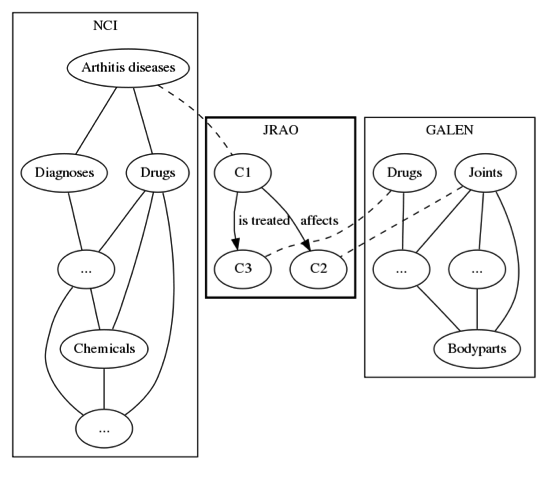
\includegraphics[width=0.6\textwidth]{useCaseOnto3.png}
\caption{JRAO  -- Example for Module Extraction}
\label{JRAO}
\end{center}
\end{figure}


\begin{lstlisting}[basicstyle=\ttfamily,language=dolText,morekeywords={props,ObjectProperty,Class,DisjointUnionOf,SubClassOf,Characteristics,Transitive,Asymmetric,SubPropertyOf,DisjointClasses,EquivalentTo,inverse,only,forall,iff,if,or,exists,distributed,extract},escapechar=@,mathescape]
library GalenModule
logic OWL
ontology myGalen = 
  http://purl.bioontology.org/ontology/GALEN extract Drugs, Joints, Bodyparts
end

module myGalenIsAModule : myGalen of http://purl.bioontology.org/ontology/GALEN 
  for Drugs, Joints, Bodyparts
end
\end{lstlisting}
 


\section{Use Case Onto-4: Interoperability Between Closed-World Data and Open-World Metadata}
Data collection has become easier and much more widespread over the years. This data has to be 
assigned a meaning somehow, which occurs traditionally in the  form of metadata annotations. For 
instance, consider geographical datasets derived from satellite data and raw sensor readings. 
Current implementations in, e.g., ecological economics\cite{bagstad_aries_2011} require manual 
annotation of datasets with the information relevant for their processes. While there have been 
attempts to standardize such information\cite{european_comission_inspire_2014}, metadata for 
datasets of simulation results are more difficult to standardize. Moreover, it is 
resource-consuming to link the data to the metadata, to ensure the metadata itself is of good 
quality and consistent, and to actually exploit the metadata when querying the data for data 
analysis. 

The data is usually represented in a database or RDF triple store, which work with a \termref{closed world assumption} on the dataset, and are not expressive enough to 
incorporate the metadata `background knowledge', such as the conditions for validity of the physical laws in the model of the object of observation. These metadata 
require a more expressive language, such as OWL or Common Logic, which operate under an open-world semantics. However, it is unfeasible to translate the 
whole large dataset into OWL or first-order logic. To `meet in the middle', it is possible to declare bridge rules (i.e., a mapping layer) that can link the metadata to 
the data. This approach can be used for intelligent data analysis that combines the data and metadata through querying the system. It enables the analysis of the 
data on the conceptual layer, instead of users having to learn the SQL/SPARQL query languages and how the data is stored. There are various tools and theories 
to realize this, which is collectively called Ontology-Based Data Access/Management, see also [OBDA].

The languages for representing the metadata or ontology, for representing the bridge rules or mapping assertions, and for representing the data are different yet 
they need to be orchestrated and handled smoothly in the system, be this for data analytics for large enterprises, for formulating policies, or in silico biology in the 
sciences. 

DOL  provides the framework for expressing such bridge rules in a systematic way, maintaining these, and building tools for them. 


\section{Use Case Onto-5: Verification of Rules Translating Dublin Core Into PROV}
The Dublin Core Metadata terms, which have been formalized as an RDF Schema vocabulary, developed initially by the digital library community, are less 
comprehensive but more widely used than PROV (cf. Use Case Onto-1). The rules for translating Dublin Core to the OWL subset of PROV (and, with restrictions, 
vice versa) are not known to yield valid instances of the PROV data model, i.e. they are not known to yield OWL ontologies consistent with respect to the OWL axioms that 
capture part of the PROV data model. This may disrupt systems that would like to reason about the provenance of an entity, and thus the assessment of the 
entity's quality, reliability or trustworthiness.
The Dublin Core to PROV ontology translation%
\footnote{\url{http://www.w3.org/TR/2013/NOTE-prov-dc-20130430/}}
  is expressed partly by a symbol mapping and partly by FOL rules. These FOL rules are implemented by CONSTRUCT patterns in the SPARQL RDF query language.%
\footnote{E.g., \url{http://www.w3.org/TR/2013/NOTE-prov-dc-20130430/\#dct-creator}} 
SPARQL has a formal specification of the evaluation semantics of its algebraic expressions, which is different from the model-theoretic semantics of the OWL and RDF Schema languages; nevertheless SPARQL CONSTRUCT is a popular and immediately executable syntax for expressing translation rules between ontologies in RDF-based languages in a subset of FOL.
DOL  not only supports the reuse of the existing Dublin Core RDF Schema and PROV OWL ontologies as modules of a distributed ontology (= OMS network), but it is also able to support the description of the FOL translation rules in a sufficiently expressive ontology language, e.g. Common Logic, and thus enable formal verification of the translation from Dublin Core to PROV.


\section{Use Case Spec-1: Modularity of Specifications}\label{spec-1}
Often specifications become so large that it is necessary to structure
them in a modular way, for human readability and maintainability, and for more efficient tool support. The lack of a standard for such
modular structuring hinders interoperability among different
development efforts and the reuse of specifications.  \DOL provides a
notion of structured modular specification that is equally applicable
to all \DOL-conforming logical languages.

Structuring pays off even for small specifications. For example, it makes
structuring a simple specification of sorting lists in the 
following way enhances both readability and potential for re-use
of specifications:

\begin{lstlisting}[basicstyle=\ttfamily\footnotesize,language=dolText,morekeywords={sort, ops, refinement, free,spec type, assoc, unit,props,op,spec,refined, via,generated, then,ObjectProperty,Class,DisjointUnionOf,SubClassOf,Characteristics,Transitive,Asymmetric,SubPropertyOf,DisjointClasses,EquivalentTo,inverse,only,forall,iff,if,or,exists,distributed,from},escapechar=@,mathescape]	
library Sorting

%% refinement from abstract sorting to insert sort

logic CASL
%right_assoc __::__
spec TotalOrder =
  sort Elem
  pred __<=__ : Elem * Elem
  forall x,y,z : Elem
  . x <= x                         %(reflexive)%
  . x <= z if x <= y /\ y <= z     %(transitive)%
  . x = y if x <= y /\ y <= x      %(antisymmetric)%
  . x <= y \/ y <= x               %(dichotomous)%
end

spec Nat =
  free type Nat ::= 0 | suc(Nat)
end

spec List =
  Nat
then
  sort Elem
  free type List ::= [] | __::__(Elem; List)
  op count : Elem * List -> Nat
  forall x,y : Elem; L : List
  . count(x,[]) = 0
  . count(x,x :: L) = suc(count(x,L))
  . count(x,y :: L) = count(x,L) if not x=y
end

spec Sorting =
  TotalOrder and List
then
  preds is_ordered : List;
        permutation : List * List
  vars x,y:Elem; L,L1,L2:List
  . is_ordered([])
  . is_ordered(x::[])
  . is_ordered(x::y::L) <=> x<=y /\ is_ordered(y::L)
  . permutation(L1,L2) <=> (forall x:Elem . count(x,L1) = count(x,L2))
then
  op sorter : List->List
  var L:List
  . is_ordered(sorter(L))
  . permutation(L,sorter(L))
hide is_ordered, permutation
end
\end{lstlisting}

In the last step, the structuring operation of hiding is used to
restrict the specification to an export interface: we hide the
predicates \texttt{is\_ordered} and \texttt{permutation}, because they
are only auxiliary and need not be implemented.


\section{Use Case Spec-2: Specification Refinements}\label{spec-2}
Formal software and hardware development methods are often used to
ensure the correct function of systems which have safety-critical
requirements or which may not be easily accessible for repair or
replacement.  Examples of such requirements can be found in
safety-critical areas such as medical systems, or in the automotive,
avionics and aerospace industries, as well as in components used by
those industries such as in microprocessor design.

Typically, a requirement specification is refined into a
design specification and then an implementation, often involving
several intermediate steps (see, e.g. the V-model [V-model], although
this does not require formal specification).  There are numerous
specification formalisms in use, including the OMG's SysML language;
moreover, often during development, the formalism needs to be changed
(e.g. from a specification to a programming language, or from a
temporal logic to a state machine). For each of these formalisms,
notions of refinement have been defined and implemented. However, the
lack of a standardized, logically sound language and methodology for
such refinement hinders interoperability among different development
efforts and the reuse of refinements.  \DOL provides the capability to
represent refinement that is equally applicable to all \DOL-conforming
logical languages, and that covers at least the most relevant of the
industrial use cases of specification refinement.

A simple example is the refinement of the (purely declarative) sorting
specification from use case in section \ref{spec-1} into a specification of a particular sorting
algorithm (for simplicity, we choose insert sort):

\begin{lstlisting}[basicstyle=\ttfamily\footnotesize,language=dolText,morekeywords={sort, ops, refinement, free,spec type, assoc, unit,props,op,spec,refined, via,generated, then,ObjectProperty,Class,DisjointUnionOf,SubClassOf,Characteristics,Transitive,Asymmetric,SubPropertyOf,DisjointClasses,EquivalentTo,inverse,only,forall,iff,if,or,exists,distributed,from},escapechar=@,mathescape]	
spec InsertSort = 
  TotalOrder and List
then
  ops insert : Elem*List -> List;
      insert_sort : List->List
  vars x,y:Elem; L:List
  . insert(x,[]) = x::[]
  . insert(x,y::L) = x::insert(y,L) when x<=y else y::insert(x,L)
  . insert_sort([]) = []
  . insert_sort(x::L) = insert(x,insert_sort(L))
 hide insert
end

refinement InsertSortCorrectness =
   Sorting refined via sorter |-> insert_sort to InsertSort
end
\end{lstlisting}
Note that hiding is essential here to make the signatures of
both specifications compatible. If we had not hidden the
predicates \texttt{is\_ordered} and \texttt{permutation}
in the \texttt{Sorting} specification, a refinement would
not have been possible, since \texttt{InsertSort} does not
implement these predicates (and it would be rather artificial
to add an implementation for them).

\medskip

Refinements can be composed. A simple example below illustrates this
by expressing that natural numbers with addition form a monoid, and
that natural numbers can be efficiently represented for implementation
as lists of binary digits, together with several equivalent ways of
composing these refinements.

\begin{lstlisting}[basicstyle=\ttfamily\footnotesize,language=dolText,morekeywords={sort, ops, refinement, free,spec type, assoc, unit,props,op,spec,refined, via,generated, then,ObjectProperty,Class,DisjointUnionOf,SubClassOf,Characteristics,Transitive,Asymmetric,SubPropertyOf,DisjointClasses,EquivalentTo,inverse,only,forall,iff,if,or,exists,distributed,from},escapechar=@,mathescape]	
spec Monoid =
 sort Elem
 ops 0 : Elem;
         __+__ : Elem * Elem -> Elem, assoc, unit 0
end

spec NatWithSuc = %mono
 free type Nat ::= 0 | suc(Nat)
 op __+__ : Nat * Nat -> Nat, unit 0 
 forall x , y : Nat . x + suc(y) = suc(x + y)
 op 1:Nat = suc(0)
end

spec Nat =
  NatWithSuc hide suc
end

spec NatBin =
generated type Bin ::= 0 | 1 | __0(Bin) | __1(Bin)

ops __+__ , __++__ : Bin * Bin -> Bin 
forall x, y : Bin 
 .  0 0 = 0  .  0 1 = 1
 .  not  (0 = 1)  .  x 0 = y 0 => x = y .  not  (x 0 = y 1)  .  x 1 = y 1 => x = y
 .  0 + 0 = 0  .  0 ++ 0 = 1 
 .  x 0 + y 0 = (x + y) 0  .  x 0 ++ y 0 = (x + y) 1
 .  x 0 + y 1 = (x + y) 1  .  x 0 ++ y 1 = (x ++ y) 0 
 .  x 1 + y 0 = (x + y) 1  .  x 1 ++ y 0 = (x ++ y) 0
 .  x 1 + y 1 = (x ++ y) 0  .  x 1 ++ y 1 = (x ++ y) 1 
end

refinement R2 =
 Nat refined via Nat |-> Bin to NatBin
end

refinement R3 =
 Monoid refined via Elem |-> Nat to
 Nat refined via Nat |-> Bin to NatBin
end

refinement R3' =
 Monoid refined via Elem |-> Nat to R2
end

refinement R3'' = 
 Monoid refined via Elem |-> Nat to Nat then R2
end

refinement R3''' = R1 then R2

\end{lstlisting}



\section{Use Case Model-1: Consistency Among UML Diagrams of Different Types}
\label{model-1}

A typical UML model involves diagrams of different types. Such UML models may have intrinsic errors because diagrams of different types may specify conflicting 
requirements. Typical questions that arise in this context are, e.g.,

\begin{itemize}
\item whether the multiplicities in a class diagram are consistent with each other;
\item wether the attributes and operations in a state machine are
available in a class diagram;
\item	  whether the sequential composition of actions in an interaction diagram is justified by an accompanying OCL specification;
\item 	whether cooperating state machines comply with pre-/post-conditions and invariants;
\item 	whether the behavior prescribed in an interaction diagram is realizable by several state machines cooperating according to a composite structure diagram.
\end{itemize}
Such questions are currently hard to answer in a systematic manner. One method to answer these questions and find such errors is a check for semantic 
consistency. Under some restrictions, the proof of semantic consistency can be (at least partially) performed using model-checking tools like Hugo/RT \cite{knapp-wuttke:models06wsh:2007}. 
Once a formal semantics for the different diagram types has been chosen (see, e.g. \cite{knapp-mossakowski-roggenbach:corr:2014}), it is possible to use \DOL to specify in which 
sense the diagrams need to be consistent, and check this by suitable tools.


\ssclause{The ATM Example}
\label{sec:atm-example}

We present as a small example in model-driven development using UML,
taken from \cite{knapp-mossakowski-roggenbach:corr:2014}.  It involves
the design of a traditional automatic teller machine (ATM) connected
to a bank. For simplicity, we only describe the handling of entering a
card and a PIN with the ATM. After entering the card, one has three
trials for entering the correct PIN (which is checked by the
bank). After three unsuccessful trials the card is kept.

\begin{figure}[!Ht]
\centering
\subfigure[Interaction\label{fig:interaction}]{%
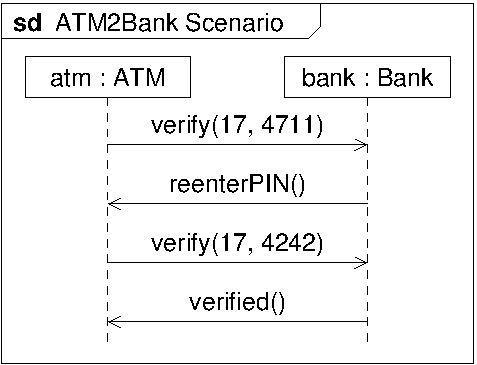
\includegraphics[scale=.5]{illustrations/uml/sd-atm2bank.pdf}
%  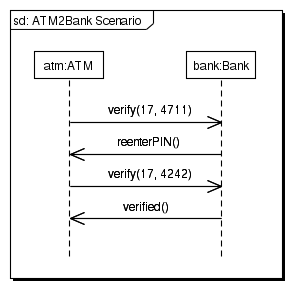
\includegraphics[trim=6 6 6 6,clip,scale=0.65]{illustrations/uml/scenario.png}%\\[-1.5ex]
}
\hspace*{0.5cm}
\subfigure[Composite structure\label{fig:system}]{%
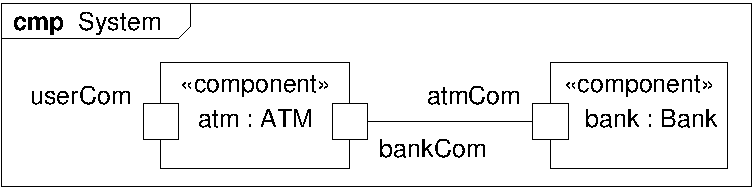
\includegraphics[scale=.5]{illustrations/uml/cmp-system.pdf}
%  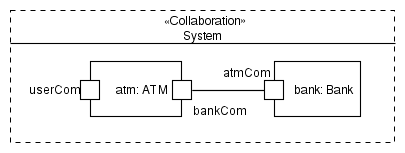
\includegraphics[trim=6 6 6 6,clip,scale=0.65]{illustrations/uml/system.png}%\\[-1.5ex]
}
\\
\subfigure[Protocol state machine\label{fig:psm}]{%
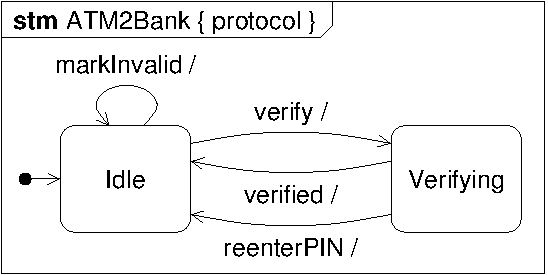
\includegraphics[scale=.5]{illustrations/uml/stm-atm2bank-protocol.pdf}
%  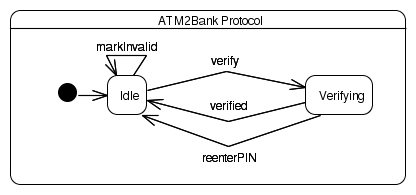
\includegraphics[trim=6 6 6 6,clip,scale=.65]{illustrations/uml/protocol.png}%\\[-1.5ex]
}
\hspace*{0.4cm}
\subfigure[Interfaces and components\label{fig:class}]{%
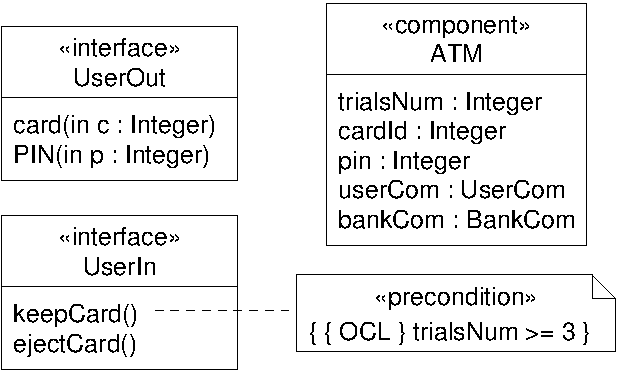
\includegraphics[scale=.5]{illustrations/uml/pkg-components.pdf}
%  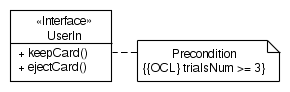
\includegraphics[trim=6 6 6 6,clip,scale=0.65]{illustrations/uml/interfaceWithOCL.png}%\\[-1.5ex]
}
\\
\subfigure[State machine\label{fig:state-machine}]{%
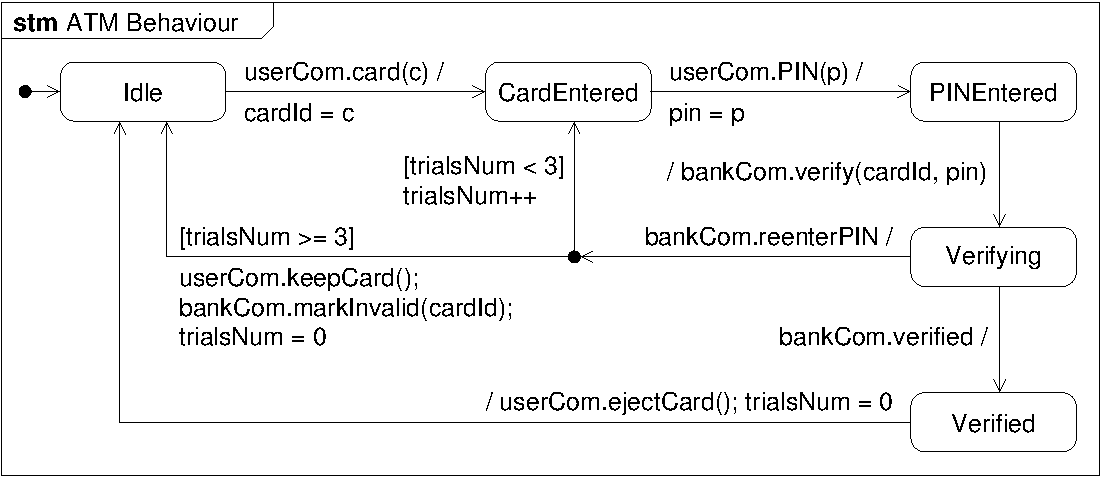
\includegraphics[scale=.5]{illustrations/uml/stm-atm-behaviour.pdf}
%  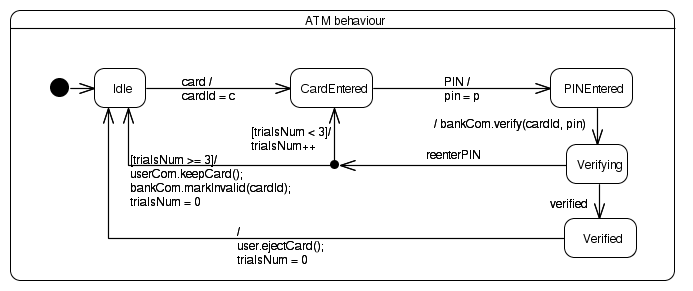
\includegraphics[trim=6 6 6 6,clip,scale=0.65]{illustrations/uml/atm-behaviour.png}%\\[-1.5ex]
}
\vspace*{-1.5ex}
\caption{ATM example}\label{fig:atm-example}
\end{figure}

Figure~\ref{fig:interaction} shows a possible \emph{interaction}
between an \uml{atm} and a \uml{bank} object, which consists of
four messages: the \uml{atm} requests the \uml{bank} to \uml{verify}
if a card and PIN number combination is valid, in the first case the
\uml{bank} requests to reenter the PIN, in the second case the
verification is successful.  This interaction presumes that the system
has an \uml{atm} and a \uml{bank} as objects. This can, e.g., be
ensured by a \emph{composite structure diagram}, see
Fig.~\ref{fig:system}, which -- among other things -- specifies the
objects in the initial system state.  Furthermore, it specifies that
the communication between \uml{atm} and \uml{bank} goes through the
two ports \uml{bankCom} and \uml{atmCom} linked by a connector.  The
communication protocol on this connector is captured with a
\emph{protocol state machine}, see Fig.~\ref{fig:psm}.  The protocol
state machine fixes in which order the messages \uml{verify},
\uml{verified}, \uml{reenterPIN}, and \uml{markInvalid} between
\uml{atm} and \uml{bank} may occur.  Figure~\ref{fig:class} provides
structural information in form of an interface specifying what is
provided at the \uml{userCom} port of the \uml{atm} instance. An
interface is a set of operations that other model elements have to
implement. In our case, the interface is described in a \emph{class
  diagram}. Here, the operation \uml{keepCard} is enriched with the
OCL constraint \uml{trialsNum >= 3}, which refines its semantics:
\uml{keepCard} can only be invoked if the OCL constraints holds.

Finally, the dynamic behaviour of the \uml{atm} object is specified by
the \emph{behavioral state machine} shown in
Fig.~\ref{fig:state-machine}. The machine consists of five states
including \uml{Idle}, \uml{CardEntered}, etc.  Beginning in the
initial \uml{Idle} state, the user can \emph{trigger} a state change
by entering the \uml{card}. This has the \emph{effect} that the
parameter \uml{c} from the \uml{card} event is assigned to the
\uml{cardId} in the \uml{atm} object (parameter names are not shown on
triggers). Entering a \uml{PIN} triggers another transition to
\uml{PINEntered}.  Then the ATM requests verification from the bank
using its \uml{bankCom} port.  The transition to \uml{Verifying} uses
a \emph{completion event}: No explicit trigger is declared and the
machine autonomously creates such an event whenever a state is
completed, i.e., all internal activities of the state are finished (in
our example there are no such activities).  If the interaction with
the bank results in \uml{reenterPIN}, and the \emph{guard}
\uml{trialsNum < 3} is true, the user can again enter a \uml{PIN}.


The ATM example in Fig.~\ref{fig:atm-example} consists of five different
models, which naturally form a network. Coherence of this network
is expressed as its consistency.
We assume that XMI representations of the
relevant UML models have been stored at
\url{http://www.example.org/uml/}, that is under URL
\url{http://www.example.org/uml/xxx.xmi}, where \url{xxx} is
determined as follows:\medskip

\begin{tabular}{|l|l|l|}\hline
\textbf{Figure} & \textbf{\texttt{xxx}} & \textbf{diagram type}\\\hline
Fig.~\ref{fig:interaction} & sd & sequence diagram\\\hline
Fig.~\ref{fig:system} & cmp & composite structure diagram\\\hline
Fig.~\ref{fig:psm} & psm & protocol state machine\\\hline
Fig.~\ref{fig:class} & cd & class diagram\\\hline
Fig.~\ref{fig:state-machine} & stm & state machine\\\hline
\end{tabular}

\begin{lstlisting}[basicstyle=\ttfamily,language=dolText,morekeywords={props,ObjectProperty,Class,DisjointUnionOf,SubClassOf,Characteristics,Transitive,Asymmetric,SubPropertyOf,DisjointClasses,EquivalentTo,inverse,only,forall,iff,if,or,exists,distributed,refinement,library,via,network,entailment,entails,refined,consistent},escapechar=@,mathescape]
%prefix( :     <http://www.example.org/uml/>
         uml:   <http://www.uml.org/spec/UML/>
%% descriptions of logics ...		 
         log:   <http://www.omg.org/spec/DOL/logics/>
library ATM

view cd2stm = cd to { atm hide along stm2cd} end
view cd2psm = cd to { psm hide along psm2cd} end
network ATM_network = %consistent
                      cd, stm, psm, cmp,
                      cd2stm, cd2psm, abstract_to_concrete_atm
entailment atm in ATM_network entails sd
network Some_refined_ATM_network = ...
refinement r = ATM_network refined to Some_refined_ATM_network
entailment e = Some_refined_ATM_network entails ATM_network
\end{lstlisting}
Here, \texttt{abstract\_to\_concrete\_atm} is defined in the next
section, and \texttt{stm2cd} and \texttt{psm2cd} are suitable logic
projections extracting the classes, attributes and operations from a
(protocol) state machine, delivering a class diagram.

\section{Use Case Model-2: Refinements Between UML Diagrams of Different Types, and Their Reuse}
\label{model-2}

A problem is a lack of reusability of refinements: Consider a controller for an elevator, which is specified with a UML protocol state machine, enriched with UML 
sequence diagrams and OCL constraints. Assume further that this model is not directly implemented, but first refined to a UML behavior state machine (which then 
can be automatically or semi-automatically transformed into some implementation using standard UML tools). However, there is no standardized language to 
express, document and maintain the refinement relation itself (UML only allows very simple refinements, namely between state machines). This hinders both the 
reuse of such refinements in different contexts, as well as the interoperability of tools proving such refinements to be correct. \DOL  
addresses these problems by providing a standardized notation with formal semantics for such refinements. Refinements expressed in this language could, e.g., be 
parameterized and reused in different contexts.

Coming to a \DOL example, we want to state the fact that the state
machine of the \uml{atm}, shown in Fig.~\ref{fig:state-machine}, is a
refinement of the protocol state machine in Fig.~\ref{fig:psm} as
follows in \DOL.  We continue the library \uml{ATM} above, again
assuming that XMI representations of the relevant UML models have been
stored at \url{http://www.example.org/uml/},
e.g.\ \url{http://www.example.org/uml/atm.xmi}:

\begin{lstlisting}[basicstyle=\ttfamily,language=dolText,morekeywords={props,ObjectProperty,Class,DisjointUnionOf,SubClassOf,Characteristics,Transitive,Asymmetric,SubPropertyOf,DisjointClasses,EquivalentTo,inverse,only,forall,iff,if,or,exists,distributed,refinement,library,via},escapechar=@,mathescape]
refinement abstract_to_concrete_atm =
  psm refined via translation psm2atm to 
       {  atm with Idle |-> Idle, CardEntered |-> Idle, 
                   PINEntered |-> Idle, Verified |-> Idle, 
                   Verifying |-> Verifying 
          hide card, PIN   }
end
\end{lstlisting}

The refinement uses an abstraction of the \uml{atm}, expressed by the
translation via symbol map \texttt{Idle |-> Idle, CardEntered |-> Idle, PINEntered |-> Idle, Verified |-> Idle, Verifying |-> Verifying}, resulting in a two-state machine. Moreover, some detail of the \uml{atm} is hidden using
\syntax{hide}. Then, the protocol state machine can be refined to
the thus abstracted \uml{atm}.

\section{Use Case Model-3: Coherent Semantics for Multi-Language Models}
\label{model-3}
	
Often a single problem area within a given domain must be represented using several formalisms, e.g., because of user community requirements, expressiveness or tool support 
and usage. 
Typically the different representations are written by different people using formalisms that are based on different logics. Thus, it is a challenge to maintain 
consistency across the different representations. 
The need for the use of multiple OMS languages, even within the OMG community, is also reflected by the OMG Ontology Definition Metamodel (ODM), which 
provides a number of syntactic transformations between such languages.
One example is the OMG Date-Time Vocabulary (DTV). DTV has been formulated in different languages, each of which addresses different audiences:
\begin{itemize}
\item	 SBVR: business users
\item 	UML (class diagrams and OCL): software implementers
\item 	OWL: ontology developers and users
\item 	Common Logic: (foundational) ontology developers and users
\end{itemize}
With \DOL, one can, e.g.,
\begin{itemize}
\item 	formally relate the different formalizations used for DTV, relate the different formalizations using translations,
\item 	check consistency across the different formalizations (using suitable tools),
\item 	extract sub-modules covering specific aspects, and
\item 	specify the OWL version to be an approximation of the Common Logic version (using a heterogeneous interpretation of OMS).
\end{itemize}
Note that the last point does not specify what information is lost in the approximation. Indeed, \DOL provides the means to specify requirements on the approximation, e.g., that it maximally preserves the information. 

Coming to a \DOL example,
a model like the ATM model developed in section \ref{sec:atm-example} typically is part of an
application context that also contains some common terminology.
This terminology often is specified by an ontology, and then
it is desirable to relate the model to the ontology. Consider
the following financial ontology fragment:

\begin{lstlisting}[basicstyle=\ttfamily,language=dolText,morekeywords={props,ObjectProperty,Class,DisjointUnionOf,SubClassOf,DisjointWith, Irreflexive, Characteristics,Transitive,Asymmetric,SubPropertyOf,DisjointClasses,EquivalentTo,inverse,only,forall,iff,if,or,exists,sort,ops,in,approximate,extract},escapechar=@,mathescape]
ontology myTaxonomy =
  ObjectProperty: owns 
    Characteristics: Irreflexive, Asymmetric

  Class: FinancialIntermediary
    SubClassOf: CorporatePerson 
  Class: CorporatePerson
    SubClassOf: ImmaterialEntity
  Class: ImmaterialEntity
    DisjointWith: MaterialEntity
    SubClassOf: has_part only ImmaterialEntity
  Class: Livestock 	
    SubClassOf: MaterialEntity 
...
end
\end{lstlisting}

When we want to relate this ontology with the ATM model, 
we need to take care of various aspects:
\begin{itemize}
  \item Translating into shared language (here, we choose Common Logic)
  \item Unifying terminology (Bank vs. FinancialIntermediary)
  \item Connecting related concepts (bank.owns.ATM vs. owns)
  \item Removing irrelevant parts (livestock) 
\end{itemize}

\begin{lstlisting}[basicstyle=\ttfamily\small,language=dolText,morekeywords={props,ObjectProperty,Class,DisjointUnionOf,SubClassOf,DisjointWith, OMS, Characteristics,Transitive,Asymmetric,translation,SubPropertyOf,DisjointClasses,EquivalentTo,inverse,only,forall,iff,if,or,exists,sort,ops,in,approximate,extract,oms,model},escapechar=@,mathescape]
model xmiStateModel = <https://ontohub.org/ATM/state.xmi>

model clStateModel = xmiStateModel with
                     translation UMLState2CL

model xmiClassModel = <https://ontohub.org/ATM/class.xmi>			

model clClassModel = xmiClassModel with 
            translation UMLClass2CL 
            Bank |-> FinancialIntermediary

ontology BigTaxonomy = <https://ontohub.org/ATM/mytaxonmy.owl>			

ontology NoLivestockTaxonomy = BigTaxonomy reject
                               Class: Livestock
						  end

ontology ExtendedTaxonomy = NoLivestockTaxonomy then 
         ObjectProperty FinancialIntermediary.owns.ATM
           SubPropertyOf: owns 
           Domain: FinancialIntermediary 
           Range: ATM
end

ontology clTaxonomy = ExtendedTaxonomy with 
                      translation OWL22CommonLogic

oms JointModel = clStateModel and 
                 clClassModel and 
                 clTaxonomy
end
\end{lstlisting}


\section{Conclusion}

In the next sections, we discuss  the metalanguage \DOL, its features that enable the support of a variety of formalisms, with syntax, well-defined semantics and model theory. \DOL 
distills best practices of modularity and metarelations (such as refinement and alignment) across the three areas of ontology design, formal 
specification, and model-driven development. It provides the ability to specify the basis for formal interoperability even among heterogeneous OMS and OMS networks. \DOL enables the solutions of the problems described in the use cases above. It also enables the development of OMS libraries, tools and workflows that 
allow  a better exchange and reuse of OMS. Eventually, this will also lead to better, easier developed and maintained systems based on these OMS.


\chapter{Design Overview} \label{c:design}
%
%\ednote{replace this section by saying how we respond to the RFP}
%
%\CLnote[type=todo]{Get rid of formal \should/\shall language (e.g.\ in clause headers: \should/\shall applies to conforming implementations anyway, rather than to this standard itself!) – not necessary in an informative clause. TM: I did this in the clause headings, and for the design part also in the clause texts.}
%
%
This clause is informative. Its purpose is to briefly describe the 
%purposes of the Distributed Ontology, Modeling and Specification Language (DOL) and 
 overall guiding principles and constraints of \DOL's syntax and semantics.
%
%\todonote{add somewhere: \DOL is a meta language and can be used with OMS languages of any expressiveness. As a Meta-language, \DOL provides a framework for combining and relating OMS written in specific OMS languages.
%However, \DOL cannot be used for writing new basic OMS.}
%
%\todonote{add ref to annex K}
%
%\section{DOL requirements}\label{c:req:overview}
%
%DOL has been designed and developed with several requirements in mind, all arising from its intended role of enabling OMS interoperability. The use of ``{\should}'' in the rest of clause 5 indicates a desired goal but is not required of \DOL (in accordance with Annex H of ISO/IEC Directives -- Part 2).
%
%\CLnote[type=todo]{give quick overview here.  Create clause 5.2 for requirements, and 5.3 for design overview. TM: done}
%
%\subsection{DOL is free, generally applicable, open, and extensible.}\label{c:req:extensible}
%
%DOL \should be
%\begin{description}
%\item[free] This \IS \should be freely available for unrestricted use.
%\item[generally applicable] It \should neither be restricted to OMS in a specific domain, nor to foundational OMS, nor to OMS represented in a specific OMS language, nor to OMS stored in any specific repositories.
%\item[open] It \should support mapping, integrating, and annotating OMS across arbitrary internet locations.  It \should make use of existing open standards wherever suitable.  The criteria for extending \DOL (see next item) \should be transparent and explicit.
%\item[extensible] It \should provide a framework into which any existing, and, desirably, any future OMS language can be plugged.
%\end{description}
%
%DOL \shall be applicable to any OMS language that has a formal, logic-based semantics or a semantics defined by translation to another OMS language with such a formal semantics. The annotation framework of \DOL \should additionally be applicable to the non-logical constructs of such languages. This \IS \todonote[author=Christoph Lange,date=D:201109221211+02'00',type=fyi]{We can afford to say ``shall'' here, as these criteria are really something that we can fully provide} \shall specify formal criteria for establishing the conformance of an OMS language with \DOL.  Annexes \shall establish the conformance of a number of relevant OMS languages with \DOL; a registry shall offer the possibility to add further (also non-standardized) languages:\CLnote[date=D:201201100956+01'00']{John Sowa: Make it modular with a simple core that can run efficiently on small systems, but can grow indefinitely to support as much as anyone could desire.}
%
%\begin{description}
%\item[normative] OWL, Common Logic, RDF Schema\todonote[author=Christoph Lange,date=D:201111021905+01'00']{RIF as well?  See \ticket{16}}
%\item[informative] F-logic,  UML class diagrams, OBO (see appendix~\ref{a:ext-graph} for a longer list)
%\end{description}
%
%\subsection{DOL is a logic-agnostic metalanguage, in the sense that its constructs can be used for many different logics.}\label{c:req:agnostic}
%
%\CLnote{here and elsewhere: remove ``shall'' from section headers}
%
%DOL \shall provide syntactic constructs for structuring OMS regardless of the logic their sentences are formalized in. \DOL \should provide syntactic constructs for
%
%\begin{itemize}
%\item basic and structured OMS (and facilities to identify them in a globally unique way),
%\item explicit extraction of modules from existing OMS, \markupcomment[author=Christoph Lange,type=q-aut]{such that, \eg, changes in the OMS can be propagated to the extracted module}{This rather sounds like a use case description to me than like a requirement.  Move it somewhere else?  Where?}.
%\item mappings between OMS (\cf \cref{c:req:links}), including interpretations, relations between OMS and their modules, as well as alignments.
%\end{itemize}
%DOL \shallnot provide its own constructs for expressing sentences.  Instead, it \shall \textit{inherit} the logical language aspects of conforming OMS languages.  It \should be possible to literally include sentences expressed in such OMS languages in a \DOL OMS.
%
%DOL \shall provide an initial set of built-in approximation methods and module extraction selectors.  Additionally, it \shall provide a means of referring to approximation methods and module extraction selectors defined externally of this \IS.\todonote[author=Christoph Lange,date=D:201111030047+01'00',type=fyi]{In practice we will use IRIs for that purpose.}
%
%DOL \shall provide an initial vocabulary for expressing relations in correspondences (as part of alignments between OMS).  Additionally, it \shall provide a means of reusing relation types defined externally of this \IS.
%
%DOL \shallnot provide an annotation vocabulary, i.e.\ it \shall neither provide annotation properties nor datatypes to be used with literal annotation objects. Instead, an informative annex \shall recommend existing annotation vocabularies for use with \DOL.
%
%\subsection{DOL has user- and machine-readable serializations.}
%
%\CLnote[type=q-all]{We need to revise this following the agreement to drop the XML and RDF serializations.}In the interest of wide applicability and tool support, \DOL \should support multiple alternative serializations.  In particular, there \should be a text serialization targeting human readers and writers, as well as serializations optimized for machine processability.
%
%This \IS \shall specify criteria for a serialization to conform with \DOL, and it \shall specify the following conforming serializations:
%
%\begin{itemize}
%\item a human-readable \textbf{text serialization}
%\item a machine-processable \textbf{interchange format}, to be implemented as
%  \begin{description}
%  \item[an XML schema (DOL XML)] particularly targeting document or form based authoring, validation, as well as translation from and to serializations of existing OMS languages\todonote[author=Christoph Lange,date=D:201204050853+02'00',type=q-all]{I think it's reasonable to call this ``DOL XML'' instead of ``DIF XML'', as to emphasize the ``brand'' \DOL}, and
%  \item[an RDF vocabulary (DOL RDF)] particularly targeting interlinking and annotation.
%  \end{description}
%\end{itemize}
%
%The \textbf{text serialization} in particular \shall offer a syntax for abbreviating identifiers of resources within OMS in a way that does not require authors to write down their full global identifiers.
%
%An OMS implemented in \DOL \should be able to comprise parts formalized in any OMS language; any serialization of \DOL \should be able to literally include such parts, regardless of the OMS language serialization they have been written in. \todonote[author=Christoph Lange,date=D:201109200256+02'00',type=fyi]{advanced namespacing is the solution that addresses this requirement} Additionally, an OMS implemented in \DOL \should be able to refer to any external OMS formalized in any OMS language, as long as they can be identified in a globally unique way.
%
%Existing OMS in existing XML serializations (\eg XCL) or text serializations (\eg OWL Manchester Syntax) \should validate as \DOL OMS with a minimum amount of syntactic adaptation. Existing OMS files/documents \should be usable in a \DOL context without the need for modification.
%
%\subsection{DOL has a well-defined formal, logic-based semantics.}\label{c:req:semantics}
%
%The structural elements and structural mappings of \DOL \should have a formal, logic-based semantics.
%
%This \IS specifies OMS language translations between conforming languages:\todonote[author=Christoph Lange,date=D:201110060000+02'00',type=fyi]{we shall establish the conformance of an initial set of languages with \DOL. As a part of that work we deliver the "onto-logical translation graph" between these languages. Anyone, who wants to establish the conformance of another language with \DOL, has to add a node to the graph, and at least one edge from/to an existing node.}
%
%\begin{itemize}
%\item OMS language translations between their logical language aspects. For any such OMS language translation its properties \should be determined, \eg whether it is a sublogic, a theoroidal translation, etc. \\
%~\todonote[author=Christoph Lange,date=D:201110060000+02'00',type=todo]{meet the requirements of people who combine OWL reasoners with Prolog. Some additional research needed on combining logics that have a model theory with those that don't}
%\item OMS language translations between their structuring language aspects and the structuring language aspect of \DOL.
%\end{itemize}
%DOL can express the application $T(O)$ of an OMS language translation $T\colon L_1\to L_2$ to an OMS $O$ written in langauge $L_1$\todonote[author=Christoph Lange,date=D:201110060000+02'00',type=fyi]{T shall be identified by a IRI. There might be multiple different possible translations between two languages, \eg two ways of expressing OWL roles in CL (binary predicate vs.\ boolean function).  But in order to free the user from always writing down such IRIs, we shall specify some defaults in our translation graph.}, see the abstract syntax category
%\syntax{Translation} in clause~\ref{c:abstract-syntax}.  \DOL need not be capable of expressing OMS language translations.
%
%\begin{figure}
%  \centering
%  \documentclass{standalone}
\usepackage[T1]{fontenc}
\usepackage[utf8]{inputenc}
\usepackage{fourier}
\renewcommand{\sfdefault}{Myriad-LF}
\usepackage[scaled=.8]{beramono}
% Minion and Myriad fonts – comment these lines if you don't have them!
% (http://lglinux.blogspot.com/2007/09/myriad-and-minion-for-latex.html)
\usepackage[minionint,mathlf]{MinionPro}
\usepackage{tikz}
\usetikzlibrary{shadows,shapes,positioning,arrows}
\tikzstyle{ontoiop}=[font=\sffamily,
    language/.style={circle,draw},
    translation/.style={-stealth'},
    dol/.style={rectangle,rounded corners,draw,align=left},
    import/.style={-o},
]
% Our colors
\definecolor{cl}{RGB}{127,129,209}
\definecolor{owl}{RGB}{138,173,72}
\definecolor{rdfs}{RGB}{232,146,31}
\definecolor{dol}{RGB}{253,246,234}
\definecolor{owlxml}{RGB}{240,251,239}
\definecolor{clif}{RGB}{242,242,251}

\begin{document}
  \begin{tikzpicture}[ontoiop]
    % Common Logic
    \node[label=Common Logic,language,fill=cl] (cl) {};
    % OWL
    \node[label=below:OWL,language,fill=owl,below left=of cl] (owl) {};
    % RDFS
    \node[label=below:RDFS,language,fill=rdfs,below right=of cl] (rdfs) {};
    \draw[translation] (owl) to (cl);
    \draw[translation] (rdfs) to (cl);
  \end{tikzpicture}
\end{document}

%  \caption{Translating two OMS languages into a third
%one}
%\label{f:DOL-translations}
%\end{figure}
%
%For each pair $L_1$ and $L_2$ of OMS languages, OMS language translations $T_1$ and $T_2$ into a common target OMS language $L_T$ \should be specified. (If $L_T$ does not exist, the only way to express a heterogeneous OMS involving $L_1$ and $L_2$ may be to keep the \DOL expression and the individual OMS in $L_1$ and $L_2$.)  These \should be translations into an OMS language that is more expressive than both $L_1$ and $L_2$, such that the union of the images of the translations is a subset of the target OMS language ($T_1(L_1)\cup T_2(L_2)\subseteq L_T$).  \fref{f:DOL-translations} outlines such an example, where Common Logic serves as the common target for OWL and RDF Schema, as it is more expressive than either of them.\todonote[author=Christoph Lange,date=D:201110060000+02'00',type=fyi]{In the context of that, specify when a document/an OMS conforms with \DOL.}  If such a target OMS language or suitable translations do not yet exist, translations into a less expressive language may be specified as an alternative, such that the intersection of the images of the translations forms a subset of the target language ($T_1(L_1)\cap T_2(L_2)\subseteq L_T$), which \should be as large as possible.  For example, an OMS language that is more expressive than both Common Logic and F-Logic does not yet exist; therefore, it would be possible to specify translations into the first-order logic subset of either OMS language.
%
%
%
%Reductions of \DOL to conforming OMS languages, as well as approximations of \DOL in conforming OMS languages, are specified.  This is to ensure that OMS that have originally been written in \DOL can be reused and extended in the respective target OMS languages. While approximations are desirable that preserve as much information from the \DOL OMS as the logic underlying the target OMS language is capable of expressing (possibly after a suitable OMS language translation), there \should at least be a trivial reduction that throws away all syntactic constructs of the \DOL OMS that are not syntactic constructs in the target OMS language. However, those constructs are optionally preserved as annotations in the output (cf. \cref{c:req:annotation} for annotations).
%
%\todonote[author=Christoph Lange,date=D:201110060000+02'00',type=todo]{provide example of integrating two OMS in a single-sorted logic by translating into many-sorted logic, where only many-sorted logic would guarantee consistency}
%
%\section{DOL design}
\label{c:design:overview}
%

We give an overview of the most important and innovative language
constructs of \DOL. Details can be found in clause~\ref{c:abstract-syntax}.

\section{DOL in a Nutshell}

As the usage scenarios in clause \ref{c:goal} illustrate, the use of multiple OMS may lead to lack 
 of interoperability. The goal of \DOL is to enable users to overcome these interoperability issues by providing a language for representing 
structured OMS and the relations between OMS as part of an OMS network in a semantically well-defined way. One particular challenge that needs to be
addressed is that OMS are written in a wide variety of OMS languages, which differ in style, 
expressivity and logical properties. 
We face this diversity not by proposing a
``universal'' language that is intended to subsume all the others, but by accepting
this pluralism in OMS languages and by formulating means (on a sound and formal semantic basis) to
 compare and integrate OMS written in different formalisms. Thus, \DOL is not `yet-another-modeling
language', but a meta-language that is used on top of existing OMS languages. 

The major functions of \DOL are the following: 
\begin{itemize}
		\item \DOL allows the use of OMS in other OMS languages (e.g., UML class diagrams, \CASL, 
		OWL, Common Logic) without requiring any changes. These are called \emph{native OMS}.  
		\item \DOL provides for defining new, \emph{structured OMS} based on existing OMS.\footnote{Also native OMS can use the structuring constructs from their OMS language. However, these structuring constructs are often quite limited, and moreover, they differ from OMS language to OMS language.} \DOL provides a number of operations for this purpose; e.g.,
		it is possible to define a structured OMS $C$ as the union of an OWL
		ontology $A$ and a Common Logic ontology $B$.
		\item \DOL provides for defining connections between two OMS by using 
		\emph{OMS mappings}. \DOL provides a variety of mappings; e.g.,  one can align terminology 
		between different OMS or specify that some OMS is an extension of another. A set of OMS
		and OMS mappings may form together an \emph{OMS network}.
		\item Native OMS inherit their semantics from the underlying OMS languages. The \DOL
		 operations for defining structured OMS, 
		OMS mappings, and OMS networks have a declarative model-theoretic semantics, which is 
		 defined in \cref{c:semantics}.  
\end{itemize}
 
The syntax of \DOL roughly follows these functions; native OMS, the various kind of structured OMS, OMS mappings, and OMS networks are the most important syntactic categories of \DOL. 
They (together with queries and importation) form the items in a \emph{DOL library}.
 





\section{Features of \DOL}\label{c:req:overview}

\DOL is a language enabling OMS interoperability. 
\DOL is
\begin{description}
\item[free] \DOL is freely available for unrestricted use.
\item[generally applicable] \DOL is neither restricted to OMS in a specific domain, nor to foundational OMS, nor to OMS represented in a specific OMS language, nor to OMS stored in any specific repositories.
\item[open] \DOL supports mapping, integrating, and annotating OMS across arbitrary internet locations.  It makes use of existing open standards wherever suitable.  The criteria for extending \DOL (see next item) are transparent and explicit.
\item[extensible] \DOL provides a framework into which any existing, and, desirably, any future OMS language can be plugged.
\end{description}
\DOL is applicable to any OMS language that has a formal, logic-based semantics or a semantics defined by translation to another OMS language with such a formal semantics. The annotation framework of \DOL is additionally applicable to the non-logical constructs of such languages. This \IS specifies formal criteria for establishing the conformance of an OMS language with \DOL.  The annex establishes the conformance of a number of relevant OMS languages with \DOL; a registry shall offer the possibility to add further (also non-standardized) languages. 

\DOL provides syntactic constructs for structuring OMS regardless of the logic their sentences are formalized in. 
Since \DOL is a meta-language,  it \textit{inherits} the logical language aspects of conforming OMS languages.  It is possible to literally include sentences expressed in such OMS languages in a \DOL OMS.


\DOL provides an initial vocabulary for expressing relations in correspondences (as part of alignments between OMS).  Additionally, it provides a means of reusing relation types defined externally of this \IS.
\DOL does not provide an annotation vocabulary, i.e.\ it neither provides annotation properties nor datatypes to be used with literal annotation objects.
% Instead, an informative annex recommends existing annotation vocabularies for use with \DOL.
%\CLnote[type=q-all]{We need to revise this following the agreement to drop the XML and RDF serializations.}In the interest of wide applicability and tool support, \DOL  supports multiple alternative serializations.  In particular, there is a text serialization targeting human readers and writers, as well as serializations optimized for machine processability.
%The \textbf{text serialization} in particular offers a syntax for abbreviating identifiers of resources within OMS in a way that does not require authors to write down their full global identifiers.
%An OMS implemented in \DOL can comprise parts formalized in any OMS language; any serialization of \DOL can literally include such parts, regardless of the OMS language serialization they have been written in. \todonote[author=Christoph Lange,date=D:201109200256+02'00',type=fyi]{advanced namespacing is the solution that addresses this requirement} Additionally, an OMS implemented in \DOL can refer to any external OMS formalized in any OMS language, as long as they can be identified in a globally unique way.
%Existing OMS in existing XML serializations (\eg XCL) or text serializations (\eg OWL Manchester Syntax) validate as \DOL OMS with a minimum amount of syntactic adaptation. Existing OMS files/documents are usable in a \DOL context without the need for modification.


%DOL does not provide a new elementary OMS language, but provides a
% layer to be used on top of existing elementary OMS languages which
% enables OMS engineers to formally express mappings between OMS written
% in different languages and stored at different Web locations. The
% purpose of such OMS networks is enabling a greater extent of
% interoperability between data and services in complex application
% settings.

%
% The following features are essential to the design of this \IS:
%
% \begin{itemize}
% \item \DOL is a language covering OMS modularity, OMS heterogeneity, and
% OMS mapping. In particular, it enables writing structured OMS
% (thereby reusing existing OMS), OMS involving different languages,
% as well as complex mappings and relations between OMS.
% \item \DOL is a declarative language with a formal semantics.
% % for modular OMS that consist of structured OMS that are possibly heterogeneous, i.e.\ are written within the same or in different OMS languages, and made available at different Web locations.
% \item \DOL provides a superset of the modularization, Web awareness and annotation facilities of a number of commonly used OMS languages, including OWL \cite{OWL2}, RDF \cite{RDF}, Common Logic \cite{ISO/IEC 24707:2007} and UML \cite{UML}.\footnote{See \cref{c:req:extensible} for details.}
% \item \DOL is an open, extensible standard that is not restricted to a fixed set of supported OMS language but specifies criteria for any existing or future OMS language to conform with \DOL.
% \item Existing OMS in languages conforming with \DOL remain as they are; they can be enriched with \DOL's modularity and annotation constructs in a non-disruptive way.
% \end{itemize}
%
% \ednote{reformulate this, see RFP}
%
%


\section{OMS Languages}
%DOL gives interoperability a formal grounding and makes heterogeneous OMS and OMS networks and services based on them amenable to checking of coherence (e.g. consistency, conservativity, intended consequences, and compliance).
 OMS languages are declarative languages for making ontological distinctions formally precise, for modeling a domain in an unambiguous way, or for expressing algebraic specifications of software.   OMS languages are distinguished by the following features:

\begin{description}
\item[Logic] Most commonly, OMS languages are based on a description logic or some other subset of first-order logic, but in some cases, higher-order, modal, paraconsistent and other logics are used.
\item[Modularity] A means of structuring an OMS into reusable parts, reusing parts of other OMS, mapping imported symbols to those in the importing OMS, and asserting additional properties about imported symbols.
\item[Annotation] A means of enabling the attachment of human-readable descriptions to OMS symbols, addressing knowledge engineers and service developers, but also end users of OMS-based services.
\end{description}
Whereas the first feature determines the expressivity of the language and the possibilities for automated reasoning (decidability, tractability, etc.), the latter two facilitate OMS engineering as well as the engineering of OMS-based software.

Acknowledging the wide tool support that conforming established languages such as OWL, RDF, Common Logic, UML, MOF, or \CASL enjoy, existing OMS in these (and any other) conforming languages remain as they are within the \DOL framework. \DOL enhances their modularity and annotation facilities to a superset of the modularity and annotation facilities they provide themselves. 
Using \DOL's modularity constructs to make statements about modules of existing OMS works by making relevant parts of these OMS, e.g., sets of axioms, identifiable, and then referring to these identifiers from \DOL statements.  \DOL's modularity constructs are semantically well-founded within a library of formal relationships between the logics underlying the different supported OMS languages.
General annotation of OMS and their parts works in a similar way.  Here, \DOL does not provide its own annotation constructs, but once more \DOL's general mechanism of making things of interest identifiable can be employed.  Once these things have been identified, the actual annotations can be added using external mechanisms such as RDF.
\ednote{Till, is this standoff markup remark up to date? TM: we promise standoff markup at various places, but we never are specific how this can be written in \DOL.\\
CL: I have now emphasized that \DOL itself doesn't do annotation but only identification, whereas annotation is left to RDF.}

\section{DOL in the Metamodeling Hierarchy}

DOL uses the metamodeling hierarchy known from model-driven engineering:
$$\xymatrix{
\Text{M4} &&&
\Text{Set \& category theory}\ar@(ul,ur)^{\Text{specified in}} \restore \\
\Text{M3} &
\Text{MOF}\ar@(ul,ur)^{\Text{conforms to}} &
\Text{EBNF}\ar@(ul,ur)^{\Text{conforms to}} &
\Text{Institutions} \ar[u]^{\Text{specified in}}
\\
\Text{M2} &
\Text{DOL metamodel} \ar[u]^{\Text{conforms to}} \ar[ur]_(0.3){\Text{conforms to}}&
\Text{OMS language metamodel}
\ar[u]_{\Text{conforms to}} \ar[ul]_(0.7){\Text{\ conforms to}} \ar[ur]_{\Text{conforms to}}
&\\
\Text{M1} & 
\Text{DOL document} \ar[r]^{\Text{contains}} \ar[u]^{\Text{conforms to}}&
\Text{specific OMS}\ar[u]^{\Text{conforms to}}&\\
}$$

The syntax of a \DOL conformant language can be written in MOF or EBNF,
which are self-describing.  The semantics of a \DOL conformant language
is its presentation as an institution. Institutions themselves are
specified in the language of set theory and category
theory.\footnote{In the future, it may be possible to specify the
  semantics of a \DOL conformant language using a semantics-based
  logical framework such as MMT. This would close the loop already at
  M3 also for the semantics.}

\section{Semantic Foundations of \DOL}\label{sem-foundations}


A large variety of OMS languages in use can be captured at an abstract level using the concept of 
\emph{institutions}\index{institution} \cite{GoguenBurstall92}.
This allows the development of results independently of the particularities of a logical system and to use the notions of institution and  logical language interchangeably. 
%We first introduce the concept of \emph{logic syntax}.
The main idea is to collect the non-logical
symbols of the language in signatures and to assign to each signature the set of sentences that can be formed with its symbols. 
For each signature, we provide means for extracting the symbols it consists of, together with their kind.
Institutions also provide a model theory, which introduces semantics for
the language and gives a satisfaction relation between the models and
the sentences of a signature.   
% The only restriction imposed is the
% satisfaction condition, which captures the idea that truth is
% invariant under change of notation (and enlargement of context) along
% signature morphisms. This relies on two further components of
% institutions: the translation of sentences along signature morphisms,
% and the reduction of models against signature morphisms (generalizing
% the notion of model reduct known from logic).

It is also possible to complement an institution with a proof theory,
introducing a derivability relation between sentences, formalized as 
an \emph{entailment system} \cite{Meseguer89}. In particular, this
can be done for all logics that have so far been in use in \DOL.


Since institutions allow the differences between OMS languages to be elided to common abstractions, 
the semantics of basic OMS is presented in a uniform way.  The semantics of structured OMS, 
OMS mappings, OMS networks, and other \DOL expressions is defined using model-theoretic constructions
on top of institutions. 


\section{DOL Enables Expression of Logically Heterogeneous OMS and Literal Reuse of Existing OMS}
DOL is a mechanism for expressing logically heterogeneous OMS. It can be used to combine sentences and structured OMS expressed in different conforming OMS languages
and logics into single documents or modules. With \DOL, sentences or structured OMS of previously existing OMS in
conforming languages can be reused by literally including them into a \DOL OMS. A minimum of wrapping constructs and other annotations (e.g., for identifying the language of a sentence) are provided. 
 See the
abstract syntax category \syntax{OMS} in
clause~\ref{c:abstract-syntax}.

A heterogeneous OMS can import several OMS expressed in different
conforming logics, for which suitable translations have been defined
in the logic graph provided in \aref{a:graph} or in an extension to it
that has been provided when establishing the conformance of some other
logic with \DOL.  Determining the semantics of the heterogeneous OMS
requires a translation into a common target language to be applied
(\cf \cref{c:semantics}).  This translation is determined via a lookup
in the transitive closure of the logic graph.  Depending on the
reasoners available in the given application setting, it can, however,
be necessary to employ a different translation.  Authors can express
which one to employ.  In a multi-step translation, it is possible to
implicitly apply as many default translations as possible, and to
concentrate on making explicit only those translations that deviate
from the default.

\section{DOL Includes Provisions for Expressing Mappings Between OMS}\label{c:req:links}

DOL provides a syntax for expressing mappings between OMS.  One use case illustrating both is sketched in  \fref{f:DOL-mapping}.  OMS mappings supported by \DOL include:
\begin{itemize}
\item imports (particularly including imports that lead to conservative extensions), see the
abstract syntax categories \syntax{OMSRef} and \syntax{ExtensionOMS} in
clause~\ref{c:abstract-syntax}.
\item interpretations (both between OMS and OMS networks), see the
abstract syntax category \syntax{IntprDefn} in
clause~\ref{c:abstract-syntax}.
\item alignments between OMS, see the
abstract syntax category \syntax{AlignDefn} in
clause~\ref{c:abstract-syntax}.
\item mappings between OMS and their modules, see the
abstract syntax category \syntax{ModuleRelDefn} in
clause~\ref{c:abstract-syntax}.
\end{itemize}
DOL uses symbol maps to express signature translations in such OMS mappings; see the
abstract syntax category \syntax{SymbolMapItems} in
clause~\ref{c:abstract-syntax}.

DOL need not be able to fully represent logical translations but is
capable of referring to them.

DOL can also be used to combine or merge OMS along such OMS mappings, see
the rule for \syntax{combination} for the abstract syntax category
\syntax{OMS} in clause~\ref{c:abstract-syntax}.

\begin{figure}
  \centering
  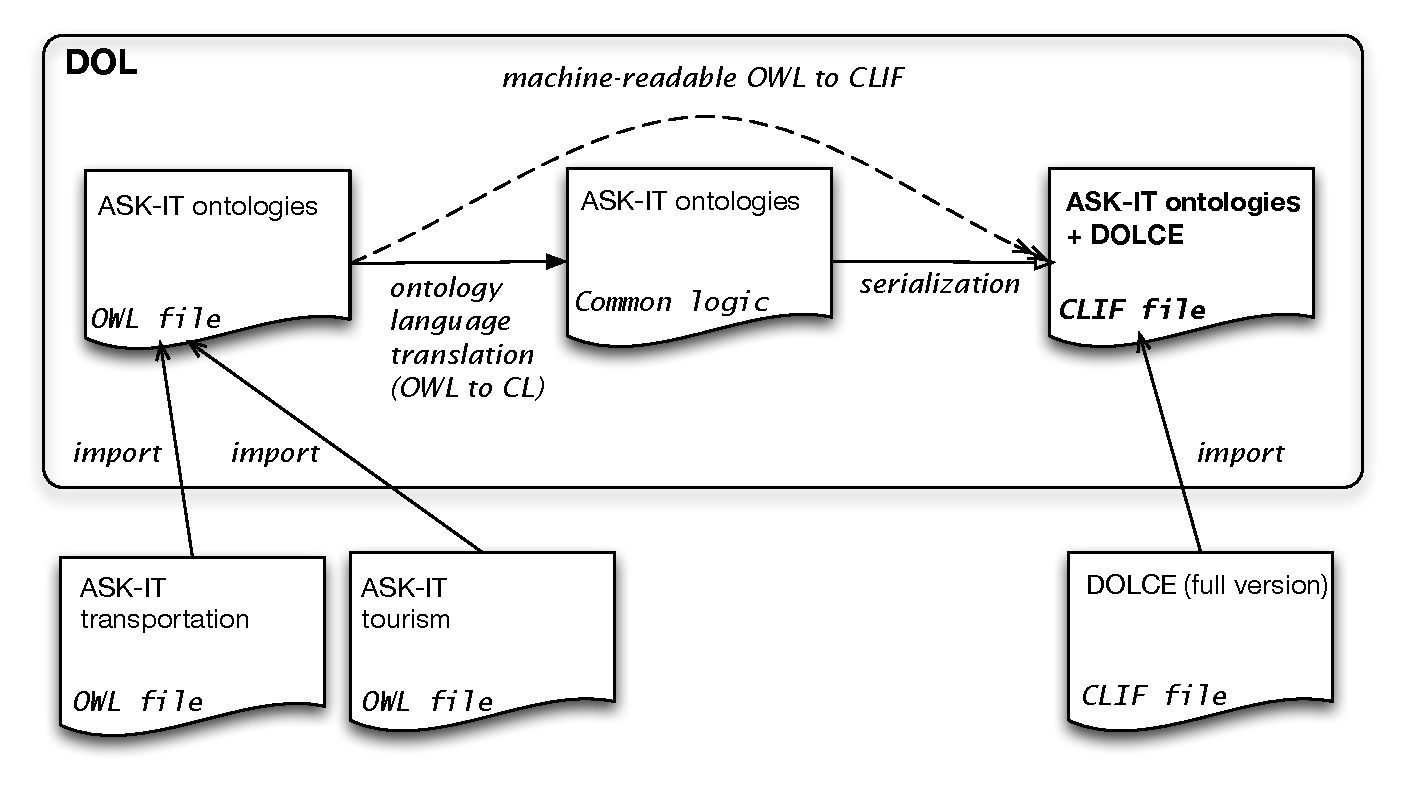
\includegraphics[width=\textwidth]{illustrations/DOLfig.pdf}
  \caption{Mapping between two OMS formulated in different OMS languages}
\label{f:DOL-mapping}
\end{figure}



\section{DOL Provides a Mechanism for Rich Annotation and Documentation of OMS}\label{c:req:annotation}

DOL provides a mechanism for identifying anything of relevance in OMS by assigning an IRI to it.  With RDF there is a standard mechanism for annotating things identified by IRIs.  Thus, \DOL supports  annotations in the full generality specified in \cref{c:terms-annotation}.

%A list of recommended RDF vocabularies for annotating OMS is presented in annex \ref{a:lola}.

\clause{DOL Abstract Syntax}\label{c:abstract-syntax}

\sclause{Abstract Syntax Categories}

DOL provides abstract syntax categories for
\begin{itemize}
\item \red{OMS} (which can be native OMS in some OMS language, or unions, translations, minimizations, combinations, approximations of OMS, among others)
\item OMS mappings 
\item OMS networks
\item \red{queries}
\item libraries (items in libraries are: definitions of OMS, OMS mappings, OMS networks and queries, as well as qualifications choosing the logic,
OMS language and/or serialization)
\item identifiers
\item annotations
\end{itemize}
 
Additionally, the categories of the abstract syntaxes of any conforming OMS languages (\cf \cref{c:conform:logic}) are also \DOL abstract syntax categories.

The following subclauses, one per abstract syntax category, specify the abstract syntax of \DOL in EBNF. Note that we deviate from the EBNF specification in
 \nisref{ISO/IEC 14977:1996} in favor of a more modern and concise
EBNF syntax.\footnote{\red{More precisely, \nisref{ISO/IEC 14977:1996} requires commas between the (non-)terminals of a right-hand side, which we omit 
for the sake of better readability. Also, we replace the separator \syntax{=}
between left and right hand-side of a rule with \syntax{::=}, and 
use the notation \syntax{N+}
for one or more repetitions of \syntax{N}.}}  
%Note that ISO EBNF lacks an operator for ``at least one repetition''.  This \IS therefore adopts the following convention: Whenever some sequence \syntax{S} is repeated at least once, we give it a non-terminal identifier of its own (\syntax{RepeatedS = S \{ S \} ;}), or group it as in \syntax{LongerExpression = Foo Bar ( S \{ S \} ) ;}.

\sclause{Libraries}\label{c:libraries}

A \termref{library} (\syntax{Library}) consists of a collection of (named)  OMS and mappings between these.  More specifically, a
library consists of a name, followed by a list of
\syntax{LibraryItem}s.  A \syntax{LibraryItem} is either a
definition of an OMS  (\syntax{OMSDefn}), 
a mapping between OMS
(\syntax{MappingDefn}), 
\red{a definition of an OMS network  (\syntax{NetworkDefn}),}
a definition related to queries 
(\syntax{QueryRelatedDefn})
or a \syntax{Qualification} selecting a specific
OMS language, logic and/or syntax that is used to interpret the
subsequent \syntax{LibraryItem}s.  Alternatively, a library can also be the verbatim inclusion of an OMS written in
an OMS language that conforms with \DOL (\syntax{NativeOMS}; \cf \ref{c:conform:logic}).

\begin{lstlisting}[language=ebnf,escapeinside={()}]  % abstract syntax

Library                  = [ PrefixMap ] , LibraryDefn
                         | NativeOMS ;
LibraryDefn              = 'library' , LibraryName , Qualification , { LibraryItem } ;
NativeOMS  = ($<$)language specific($>$) ;
LibraryItem              = LibImport | OMSDefn | NetworkDefn | MappingDefn | QueryRelatedDefn | Qualification ;
LibImport                = 'lib-import' , LibraryName ;
Qualification            = LanguageQual | LogicQual | SyntaxQual ;
LanguageQual             = 'lang-select' , LanguageRef ;
LogicQual                = 'logic-select' , LogicRef ;
SyntaxQual               = 'syntax-select' , SyntaxRef ;
LibraryName              = IRI ;

PrefixMap        = 'prefix-map' , { PrefixBinding } ;
PrefixBinding    = 'prefix-binding' , BoundPrefix , IRIBoundToPrefix ,
                   [ Separators ] ;
BoundPrefix      = 'bound-prefix' , [ Prefix ] ;
IRIBoundToPrefix = 'full-iri' , FullIRI ;
Separators       = 'separators' , LibraryOMSSeparator , OMSSymbolSeparator ;
LibraryOMSSeparator = SeparatorString ;
OMSSymbolSeparator  = SeparatorString ;
SeparatorString  = SeparatorChar , { SeparatorChar } ;
SeparatorChar    = ipchar | gen-delims , - , '#' ;
                   ($<$ \rm as defined in \nisref{IETF/RFC 3987} $>$)
\end{lstlisting}
%% ~\todonote[type=fyi,author=Christoph Lange]{Things changed from HetCASL:\textLF
%%   • logic-select now mandatory (no default logic) and tree-scoped MC: what does this mean? To make Hets-lib conform with this, we should have .het files equivalent to .dol files with logic selected to be CASL\textLF
%%   • download-items (encourage linked data best practices instead)\textLF
%%   • item-name-map (to be replaced by namespaces??)\textLF
%%   • lib-version (to be replaced by metadata annotations, \eg OMV)\textLF
%%   • indirect-mapping (will always use full IRIs, and abbreviate them by syntactic namespaces)}

At the beginning of a library, one can declare a \syntax{PrefixMap} for abbreviating long IRIs; see \cref{c:identifiers} for further details.

\sclause{OMS Networks}\label{c:networks}
\red{
Inside a library, one can define OMS networks (\syntax{NetworkDefn}).
A \syntax{NetworkDefn} names an
OMS network consisting of  OMS and OMS mappings. OMS networks may build on previously-defined
OMS networks, and they can be used in \syntax{combination}s.  
}
\begin{lstlisting}[language=ebnf,escapeinside={()}]  % abstract syntax

NetworkDefn            = 'network-defn', NetworkName , [ ConsStrength ] , Network ;
NetworkName            = IRI ;
Network                = 'network', NetworkElements , ExcludeExtensions ;
NetworkElements        = 'network-elements' , { NetworkElement } ;
NetworkElement         = 'network-element' , [ Id ] , OMSOrMappingorNetworkRef ;
ExcludeExtensions    = 'exclude-imports' , { ElementRef } ; 
ElementRef   = 'path', OMSOrMappingorNetworkRef, OMSOrMappingorNetworkRef 
               | OMSOrMappingorNetworkRef ;
OMSOrMappingorNetworkRef  = IRI ;
\end{lstlisting}

An OMS network by default also includes all inclusions (generated by
\syntax{ExtensionOMS}) between the involved OMS---unless these are
explicitly excluded.

\sclause{OMS}\label{c:focused-OMS}

An OMS (\syntax{OMS}) can be one of the following:
\begin{itemize}
\item a basic OMS \syntax{BasicOMS} written inline, in a conforming serialization of a conforming OMS 
language (which is defined outside this standard)\footnote{In this place, any OMS in a conforming serialization of a conforming OMS language is permitted.  
However, \DOL's module sublanguage should be given preference over the module sublanguage of 
the respective conforming OMS language; \eg \DOL's extension construct should be preferred over OWL's import construct.},
\item a translation of an OMS into a different signature or OMS
language,
\item a reduction of an OMS to a smaller signature and/or less
expressive logic (that is,
some non-logical symbols are hidden, but the semantic effect of sentences involving these is kept),
\item a module extracted from an OMS, using a restriction signature,
\item an approximation of an OMS, in a subsignature or sublogic, with the effect that sentences not expressible in the subsignature resp.\ sublogic are replaced with a suitable approximation,
\item \red{a filtering of an OMS, with the effect that some signature symbols and axioms are removed from the OMS,}
\item an extension of an OMS with a basic or a minimizable OMS, optionally named and/or marked as conservative, monomorphic, definitional, weakly definitional or implied,
\item a union of several OMS (the major difference between a union and extension is that the members of the unions need to be self-contained OMS, while the extensions may reuse the signature of the extended OMS), 
\item a reference to an OMS existing on the Web,
\item an OMS qualified with the OMS language that is used to express it,
\item a combination of an OMS network (technically, this is a colimit, see \cite{ZimmermanEtAl06}),
\item a minimization of an OMS, forcing the subsequently declared
  non-logical symbols to be interpreted in a minimal way, while the non-logical symbols declared so far are fixed (alternatively, the non-logical symbols to be minimized and to be varied can be explicitly declared). \red{Variants are
maximization, freeness (minimizing also data sets and equalities on these), and cofreeness
(maximizing also data sets and equalities on these),}
\item \red{the application of a substitution to an OMS.}


\end{itemize}
% derived from CASL (see CASL reference manual)
% and HetCASL (see HetCASL summary)

\begin{lstlisting}[language=ebnf,escapeinside={()}]  % abstract syntax

BasicOMS = ($<$)language specific($>$) ;
MinimizableOMS       = BasicOMS
                     | 'oms-ref' , OMSRef , [ ImportName ] ;
ExtendingOMS         = MinimizableOMS
                     | MinType , MinimizableOMS ;
OMS                  = ExtendingOMS
                     | 'minimize-symbols' , OMS , Minimization
                     | 'translation' , OMS , Translation
                     | 'reduction' , OMS , Reduction
                     | 'module-extract' , OMS , Extraction 
                     | 'approximation' , OMS , Approximation
                     | 'filtering', OMS, Filtering
                     | 'union' , OMS , [ ConsStrength ] , OMS 
                     | 'extension' , OMS , ExtensionOMS 
                     | 'qual-oms' , { Qualification } , OMS
                     | 'combination' , Network
                     | 'application', OMS, SubstName ;

Minimization         = MinType, CircMin , CircVars ;
MinType              = 'minimize' | 'maximize' | 'free' | 'cofree' ;
CircMin              = Symbol , { Symbol } ;
CircVars             = { Symbol } ;

Translation          = 'renaming' , { LogicTranslation } , [ SymbolMapItems ] ;
LogicTranslation     = 'logic-translation' , OMSLangTrans ;

Reduction            = 'hidden' , { LogicReduction } , [ SymbolItems ]
                     | 'revealed' , SymbolItems  ;
LogicReduction       = 'logic-reduction' , OMSLangTrans ;

SymbolItems          = 'symbol-items' , Symbol , { Symbol } ;
SymbolMapItems       = 'symbol-map-items' , SymbolOrMap , { SymbolOrMap } ;

Extraction           = 'extraction', QualInterfaceSignature ;

Approximation        = 'approx' , [ QualInterfaceSignature ] , [ LogicRef ] ;

Filtering            = 'select' , BasicOMS 
                     | 'reject' , BasicOMS ;

ExtensionOMS         = extension-oms , [ ExtConsStrength ] , [ ExtensionName ] , 
                                       ExtendingOMS ;

ConsStrength         = Conservative 
		     | 'monomorphic'  
		     | 'weak-definitional' 
		     | 'definitional' ;

ExtConsStrength      = ConsStrength | 'implied' ;

Conservative         = 'consequence-conservative' | 'model-conservative' 
                     | 'not-consequence-conservative' | 'not-model-conservative' ;

QualInterfaceSignature   = 'keep-signature' , InterfaceSignature 
                         | 'remove-signature' , InterfaceSignature ;

InterfaceSignature   = SymbolItems ;
ImportName           = IRI ;
ExtensionName        = IRI ;
\end{lstlisting}
%% \ednote{Alternatively, we could use one type of \syntax{InterfaceSignature}
%% only, and instead use different constructors for \syntax{Extraction}
%% and \syntax{Approximation}. This would be a bit more verbose, but a bit
%% more coherent with position of non-terminals in the concrete syntax.}

An OMS definition \syntax{OMSDefn} names an  OMS.  

It can be
optionally marked as inconsistent, consistent, monomorphic or having a unique model using 
\syntax{ConsStrength}.\footnote{More precisely, \syntax{'consequence-conservative'}
here requires the OMS to have only tautologies as signature-free logical consequences, while \syntax{'not-consequence-conservative'} expresses that this is not the case. 
\syntax{'model-conservative'}
requires satisfiability of the OMS, \syntax{'not-model-conservative'} its
unsatisfiability.
\syntax{'definitional'} expresses the unique model property; this may be interesting for characterizing
OMS (e.g.\ returned by model finders) that are used to describe single models.}. An
\syntax{SymbolItems}, used in an OMS \syntax{Reduction}, is a
list of non-logical symbols that are to be hidden. A \syntax{LogicReduction}
denotes a logic reduction to a
less expressive OMS language. A \syntax{SymbolMapItems}, used in
OMS \syntax{Translation}s,  maps symbols to symbols,
%% \CLnote[type=fyi]{On 2012-07-18 we decided 
%% not to specify lambda-style symbol-to-term mappings for now.  Would be convenient, but specifying its semantics 
%% in an OMS language independent way would require additional institution infrastructure – and the same effect can be 
%% achieved by auxiliary definitional extensions, cf.\ Colore (so promote this, informatively, as a ``best practice''?) TM: Alternatively, we could use a recent notion of institutional monad. This builds an extended signature with all terms. Then one can use ordinary signature morphisms into such extended signatures.} 
%or a logic
%translation. 
An OMS language translation \syntax{OMSLangTrans} 
can be either specified by its name, or be inferred as the \termref{default
translation} to a given target (the source will be inferred as the 
OMS language of the current OMS).

\begin{lstlisting}[language=ebnf,escapeinside={()}]  % abstract syntax

OMSDefn          = 'oms-defn' , OMSName , [ ConsStrength ] , OMS ;
Symbol           = IRI ;
SymbolMap        = 'symbol-map' , Symbol , Symbol ;
SymbolOrMap      = Symbol | SymbolMap ;
Term             = ($<$)an expression specific to an OMS language($>$) ;
Sentence         = ($<$)an expression specific to an OMS language($>$) ;
                 
OMSName          = IRI ;
                 
OMSRef           = IRI ;
ExtensionRef     = IRI ;
                 
LoLaRef          = LanguageRef | LogicRef ;
                 
LanguageRef      = IRI ;
LogicRef         = IRI ;
SyntaxRef        = IRI ;
                 
OMSLangTrans     = 'named-trans' , OMSLangTransRef
                 | 'default-trans' , LoLaRef ; 
                 
OMSLangTransRef  = IRI ;
                 
\end{lstlisting}


\sclause{OMS Mappings}\label{c:oms-mappings}

An OMS mapping provides a connection between two OMS. An OMS mapping definition is the definition of 
either a named interpretation (\syntax{IntprDefn}, \red{\syntax{Entailment}} or 
\syntax{EquivDefn}), a named declaration of the  relation between a module of an OMS and the whole 
OMS (\syntax{ModuleRelDefn}), or a named \termref{alignment} (\syntax{AlignDefn}).

The \syntax{SymbolMapItems} in an interpretation always must lead to a signature morphism; a proof 
obligation expressing that the (translated) source OMS logically follows from the target OMS is 
generated.  \red{An entailment is a variant where all symbols are mapped identically, while an 
equivalence states that the model classes of two OMS are in bijective correspondence.}

\red{
Interpretations, entailments and equivalences between OMS networks are also possible. An 
interpretation between OMS networks has to specify both a mapping between the nodes of the OMS 
network, as well as, for each node, a symbol map from the OMS of that node to the target OMS to 
which it is mapped.
%\ednote{In equivalences between OMS networks, should we allow for node mappings 
%as well? In  \cite{MossakowskiTarlecki09}, this is allowed.
%--- No, since we do not allow for signature morphisms either.}
}

In contrast to this functional style of mapping symbols, an alignment provides a relational 
connection between two OMS,  using a set of \syntax{Correspondence}s. Each correspondence may relate 
some OMS non-logical symbol to another one (possibly given by a term) with an optional confidence 
value. Moreover, the relation between the two non-logical symbols can be explicitly
specified (like being equal, or only being subsumed) in a similar way to the Alignment API \cite{AlignmentAPI}. 
\red{The relations that can be used in a correspondence are equivalence, disjointness, subsumption, membership (the last two with a
variant for each direction) or a user-defined relation that is stored in a registry and must be prefixed with
\url{http://www.omg.org/spec/DOL/correspondences/}.
A default correspondence can be used; it is applied to all pairs of non-logical symbols with 
the same local names. The default relation in a correspondence is equivalence, unless  a different 
relation is specified in a surrounding 
'CorrespondenceBlock'.
Using an \syntax{AlignCard}, left and right injectivity and totality of the
\termref{alignment} can be specified (the default is left-injective, right-injective, left-total  and right-total).
With \syntax{AlignSem}, different styles of networks of aligned ontologies (to be interpreted in 
a logic-specific way) of alignments can be specified: whether a single domain is assumed, all domains are embedded into a global domain,
or whether several local domains are linked (``contextualized'') by relations.}

A \syntax{ModuleRelDefn} declares that a certain OMS
actually is a module of some other OMS with respect
to the \syntax{InterfaceSignature}.


\begin{lstlisting}[language=ebnf,escapeinside={<>},mathescape]  % abstract syntax

MappingDefn          = IntprDefn | Entailment | EquivDefn | ModuleRelDefn | AlignDefn;

IntprDefn            = 'intpr-defn' , IntprName , [ Conservative ] , 
                        IntprType , { LogicTranslation } , [ SymbolMapItems ]                     
                     | 'refinement' , IntprName , Refinement ;
IntprName            = IRI ;
IntprType            = 'intpr-type' , OMS , OMS ;

Refinement           = 'ref-oms' , OMS 
                     | 'ref-network' , Network
                     | 'ref-composition' , Refinement , Refinement
                     | 'simple-oms-ref' , OMS , RefMap , Refinement 
                     | 'simple-network-ref' , Network , RefMap , Refinement ;
RefMap               = 'refmap-oms' , [ LogicTranslation ] , [ SymbolMapItems ] 
                     | 'refmap-network' , { NodeMap } ;
NodeMap              = 'node-map', OMSName , OMSName , 
                                   { LogicTranslation } , [ SymbolMapItems ] ;


Entailment           = 'entailment' , EntailmentName , EntailmentType ;
EntailmentType       = 'oms-oms-entailment', OMS , OMS 
                     | 'network-oms-entailment', Network , OMSName , OMS 
                     | 'network-network-entailment', Network, Network ;
EntailmentName       = IRI ;

EquivDefn            = 'equiv-defn' , EquivName , EquivType ;
EquivName            = IRI ;
EquivType            = 'oms-equiv' , OMS , OMS , OMS
                     | 'network-equiv' , Network , Network , Network ;

ModuleRelDefn        = 'module-defn' , ModuleName , [ Conservative ] , ModuleType ,
                                       InterfaceSignature ;
ModuleName           = IRI ;
ModuleType           = 'module-type' , OMS , OMS ;

AlignDefn            = 'align-defn' , AlignName , [ AlignCard ] , AlignType, 
                                    AlignSem,   { Correspondence } ; <\footnote{Note that this grammar uses ``type'' as in ``the type of a function'', whereas the Alignment API uses ``type'' for
	 the totality/injectivity of the relation/function.  For the latter, this grammar uses ``cardinality''.}>
AlignName            = IRI ;
AlignCards           = AlignCardForward , AlignCardBackward ; 
AlignCardForward     = 'align-card-forward' , AlignCard ;
AlignCardBackward    = 'align-card-backward' , AlignCard ;
AlignCard            = 'injective-and-total'
                     | 'injective'
                     | 'total'
                     | 'neither-injective-nor-total' ;
AlignType            = 'align-type' , OMS , OMS ;
AlignSem            = 'single-domain' 
                    | 'global-domain' 
                    | 'contextualized-domain' ; 

Correspondence       = CorrespondenceBlock
                     | SingleCorrespondence
                     | 'default-correspondence' ; 

CorrespondenceBlock  = 'correspondence-block' , [ RelationRef ] , [ Confidence ],
                                                Correspondence, { Correspondence } ; 
SingleCorrespondence = 'correspondence' , SymbolRef , [ RelationRef ] , [ Confidence ] ,
                                          TermOrSymbolRef , [ CorrespondenceID ] ;
CorrespondenceID     = IRI ;
SymbolRef            = IRI ;
TermOrSymbolRef      = Term | SymbolRef ;
RelationRef          = 'subsumes' | 'is-subsumed' | 'equivalent' | 'incompatible' 
                     | 'has-instance' | 'instance-of' | 'default-relation' | IRI ; 
Confidence           = Double ;
\end{lstlisting}
\begin{lstlisting}[language=ebnf,escapeinside={()},mathescape]  % abstract syntax

Double               = ($<$ a number $\in [0,1]$ $>$) ;
\end{lstlisting}

A symbol map in an interpretation is \required to cover all non-logical symbols of the source OMS; 
the semantics specification in \cref{c:semantics} makes this assumption\footnote{Mapping a 
non-logical symbol twice is an error. Mapping two source non-logical symbols to the same target 
non-logical symbol is legal, this then is a non-injective OMS mapping.}. 

%Alignments 

\sclause{Queries}
\red{
Queries are a means to extract information from an OMS.  \DOL's \syntax{QueryDefn}s cover 
``select''-type queries that deliver an answer substitution for the query variables. (Answer) 
substitutions can be stored separately, using a \syntax{SubstDefn}. A
\syntax{ResultDefn} expresses that certain answer substitutions are
the result of a query. Optionally, a result can be expressed to be
complete, meaning that it comprises all answer substitutions to the query.
}
\begin{lstlisting}[language=ebnf,escapeinside={<>},mathescape]  % abstract syntax

QueryRelatedDefn     = QueryDefn | SubstDefn | ResultDefn ;
QueryDefn            = 'select-query-defn', QueryName, Vars, Sentence, 
                                            OMS, [OMSLangTrans] ;
SubstDefn            = 'subst-defn', SubstName, OMS, OMS, SymbolMap ;
ResultDefn           = 'result-def', ResultName, SubstName, { SubstName }, 
                                     QueryName, [ Complete ] ;
QueryName            = IRI ;
SubstName            = IRI ;
ResultName           = IRI ;
Vars                 = { Symbol } ;
Complete             = 'complete' ;
\end{lstlisting}

%%%%%%%%%%%%%%%%%%%%%%%%%%%%%%%%%%%%%%%%%%%%%%%%%%%%%%%%%%%%%%%%%%%%%%%%

%~\CLnote{some text that was left over here, but I don't recall what we meant by it: recommendations for dealing with OMS language dialects}

\sclause{Identifiers}\label{c:identifiers}

This section specifies the abstract syntax of identifiers of \DOL OMS and their elements.

\ssclause{IRIs}\label{c:iris}

In accordance with best practices for publishing OMS on the Web, identifiers of OMS and their 
elements \should not just serve as \emph{names}, but also as \emph{locators}, which, when 
dereferenced, give access to a concrete representation of an OMS or one of its elements.  (For the 
specific case of RDF Schema and OWL OMS, these best practices are documented in 
\cite{W3C:NOTE-swbp-vocab-pub-20080828}.  The latter is a specialization of the linked data 
principles, which apply to any machine-processable data published on the Web 
\cite{BernersLee:LinkedData2006}.)  It is recommended that publicly accessible \DOL OMS be published 
as linked data.

%\todonote[type=q-aut,author=Christoph Lange]{Does this motivation/justification sound reasonable to 
%you? --- Yes.}
Therefore, in order to impose fewer conformance requirements on applications, \DOL requires the use of
 IRIs for identification per \nisref{IETF/RFC 3987:2005}.
  It is \recommended that libraries use 
IRIs that translate to URLs when applying the algorithm for mapping IRIs to URIs specified in 
\nisref{IETF/RFC 3987:2005, Section 3.1}.  \DOL descriptions of any element of a library that is 
identified by a certain IRI \should be \emph{located} at the corresponding URL, so that agents can 
locate them.  As IRIs are specified with a concrete syntax only in \nisref{IETF/RFC 3987:2005}, \DOL 
adopts the latter into its abstract syntax as well as all of its concrete syntaxes 
(serializations).
%\CLnote[type=q-all]{I meant to say: for IRIs, the abstract syntax is the same as 
%the concrete syntax.}.

%% We don't do "semantic namespaces" for now.  (Agreed in 2012-02-23 meeting)
% For identification, \DOL preferably employs IRIs that have the following three components:\footnote{This IRI syntax has originally been designed by Florian Rabe and Michael Kohlhase \cite{Rabe:MMT2011}, independently from this \IS.\todonote[type=todo,author=Christoph Lange]{if we leave this reference in place, we might additionally refer to the paper that describes the semantics of MMT and provides more design rationale background}}

% \begin{description}
% \item[namespace] an IRI that identifies the complete OMS
% \item[module] a name that identifies a module within an OMS
% \item[symbol] a name that identifies a non-logical symbol, named import, or sentence within a module\todonote[type=todo,author=Christoph Lange]{list the other things we would like to identify in this component}
% \end{description}
% It is recommended that these ``DOL IRIs'' be used whenever an OMS or a module of an OMS is primarily implemented in \DOL.

In accordance with semantic web best practices such as the OWL Manchester Syntax 
\cite{W3C:NOTE-owl2-manchester-syntax-20091027}, this \IS does not allow relative IRIs, and does 
not offer a mechanism for defining a base IRI, against which relative IRIs could be resolved.

Concerning these languages, note that they allow arbitrary IRIs in principle, but in practice they 
strongly recommend using IRIs consisting of two components \cite{W3C:NOTE-swbp-vocab-pub-20080828}:
\begin{description}
\item[namespace] an IRI that identifies an OMS,\footnote{See annex~\ref{a:loc/id} for a specific linked-data compliant URL scheme for \DOL.}
usually ending with \syntax{\#} or \syntax{/}
\item[local name] a name that identifies a non-logical symbol within an OMS
\end{description}

\begin{lstlisting}[language=ebnf,escapeinside={()}]  % abstract syntax

IRI     = 'full-iri' , FullIRI | 'curie' , CURIE ; (\footnote{specified below in \cref{c:curies}}) 
FullIRI = ($<$ as defined by the IRI production in \nisref{IETF/RFC 3987:2005} $>$) ;
\end{lstlisting}

\ssclause{Abbreviating IRIs using CURIEs}\label{c:curies}

As IRIs tend to be long, and as syntactic mechanisms for abbreviating them have been standardized, 
it is \recommended that applications employ such mechanisms and support expanding abbreviatory
notations into full IRIs.  For specifying the \emph{semantics} of \DOL, this \IS assumes full IRIs 
everywhere, but the \DOL abstract \emph{syntax} adopts CURIEs (compact URI expressions) as an 
abbreviation mechanism, as it is the most flexible one that has been standardized to date.  

The CURIE abbreviation mechanism works by binding prefixes to IRIs.  A CURIE consists of a 
\emph{prefix}, which may be empty, and a \emph{reference}.  If there is an in-scope binding for the 
prefix, the CURIE is valid and expands into a full IRI, which is created by concatenating the IRI 
bound to the prefix and the reference.

DOL adopts the CURIE specification of RDFa Core 1.1 \nisref{W3C/TR REC-rdfa-core:2013, Section 6} with the following changes:
\begin{itemize}
\item \DOL does not support the declaration of a ``default prefix'' mapping %\CLnote[type=q-aut]{Are such explanatory notes OK here? --- Yes}
(covering CURIEs such as \syntax{:name}).
\item \DOL does support the declaration  of a ``no prefix'' mapping (covering CURIEs such as 
\syntax{name}). \red{If there is no explicit declaration for the ``no prefix'', it defaults to a 
context-sensitive expansion mechanism, which always prepends the library IRI (in the context of a 
structured OMS where named OMS are referenced) resp.\ the current OMS IRI (in the context of a basic
OMS) to a symbol name. Both the separator between the library and the OMS name and that between the 
OMS name and the symbol name can be declared (using the keyword \syntax{separators}), and both default to ``//''.}

\item \DOL does not make use of the \syntax{safe\_curie} production.
\item \DOL does not allow binding a relative IRI to a prefix.
\item Concrete syntaxes of \DOL are encouraged but \notrequired to support CURIEs.\footnote{This is 
a concession to having an RDF-based concrete syntax among the normative concrete syntaxes.  RDFa is 
the only standardized RDF serialization to support CURIEs so far.  Other serializations, such as 
RDF/XML or Turtle, support a subset of the CURIE syntax, whereas some machine-oriented 
serializations, including N-Triples, only support full IRIs.}
\end{itemize}

CURIEs can occur in any place where IRIs are allowed, as stated in \cref{c:iris}.  Informatively, 
we can restate the CURIE grammar supported by \DOL as follows:
\begin{lstlisting}[language=ebnf,escapeinside={()}]
CURIE     = MaybeEmptyCURIE , - ;
MaybeEmptyCURIE = [ Prefix ] , RefWithoutComma ;
RefWithoutComma = Reference , - , StringWithComma ;
StringWithComma = { UChar } , ',' , { UChar } ;
UChar     = ($<$ any Unicode \nisref{ISO/IEC 10646} character $>$) ;
Prefix    = NCName , ':' ; ($<$ \rm see ``NCName'' in \nisref{W3C/TR REC-xml-names:2009}, Section 3 $>$)
Reference = Path , [ Query ] , [ Fragment ] ;
Path      = ipath-absolute | ipath-rootless | ipath-empty ;
            ($<$ \rm as defined in \nisref{IETF/RFC 3987} $>$)
Query     = '?' , iquery ; ($<$ \rm as defined in \nisref{IETF/RFC 3987} $>$)
Fragment  = '#' , ifragment ; ($<$ \rm as defined in \nisref{IETF/RFC 3987} $>$) 
\end{lstlisting}
%\ednote{This is concrete syntax. Shouldn't it be moved to chapter \ref{{a:text-syntax}}? --- I have copied it there, altough this is code
%duplication.}

Note that outside the context of a basic OMS the prefix/reference separator of a CURIE is always the colon (\syntax{:}); only for serializations of OMS languages other than \DOL it may be redefined as stated in \cref{c:conform:serialization}.

Prefix mappings can be defined at the beginning of a library (specified in \cref{c:libraries}; 
these apply to all parts of the library, including basic OMS as clarified in \cref{c:map-ids}).  
%Their syntax is:

Bindings in a prefix map are evaluated from left to right.  Authors \shouldnot bind the same prefix twice, but if they do, the later binding wins.

\ssclause{Mapping identifiers in basic OMS to IRIs}\label{c:map-ids}

While \DOL uses IRIs as identifiers throughout, OMS languages do not necessarily do; for example:
\begin{itemize}
\item OWL \nisref{W3C/TR REC-owl2-syntax:2009, Section 5.5} does use IRIs.
\item Common Logic \nisref{ISO/IEC 24707:2007} supports them but does not enforce their use.
\item F-logic \cite{flogic} does not use them at all.
\end{itemize}
However, \DOL OMS mappings as well as 
%\CLnote[type=todo]{maybe clarify which ones, by checking the grammar for all occurrences of SymbolRef}
certain operations on OMS require making unambiguous references to non-logical symbols of basic OMS (\syntax{SymbolRef}).  Therefore, \DOL provides a function that maps global identifiers used within basic OMS to IRIs.  This mapping affects all non-logical symbol identifiers (such as class names in an OWL ontology), but not locally-scoped identifiers such as bound variables in Common Logic ontologies.  \DOL reuses the CURIE mechanism for abbreviating IRIs for this purpose (\cf \cref{c:curies}).

The IRI of a non-logical symbol identifier in a basic OMS $O$ is determined by the following function:
\begin{algorithmic}
  \REQUIRE $D$ is a library
  \REQUIRE $O$ is a basic OMS in serialization $S$
  \REQUIRE $\mathit{id}$ is the identifier in question, identifying a symbol in $O$ according to the specification of $S$
  \ENSURE $i$ is an IRI
  \IF{$\mathit{id}$ represents a full IRI according to the specification of $S$}
    \STATE $i\leftarrow\mathit{id}$
  \ELSE
    \STATE \COMMENT{first construct a pattern $\mathit{cp}$ for CURIEs in $S$, then match $\mathit{id}$ against that pattern}
    \IF{the declaration of \DOL-conformance of $S$ redefines the prefix/reference separator character $\mathit{cs}$ (cf.\ \cref{c:conform:serialization})}
      \STATE $\mathit{sep}\leftarrow \mathit{cs}$
    \ELSIF{$S$ forbids prefixed CURIEs}
      \STATE $\mathit{sep}\leftarrow\text{undefined}$
    \ELSE
      \STATE $\mathit{sep}\leftarrow\mathit{:}$ \COMMENT{the standard CURIE separator character}
    \ENDIF
    \STATE \COMMENT{The following statements construct a modified EBNF grammar of CURIEs; see \nisref{ISO/IEC 14977:1996} for EBNF, and \cref{c:curies} for the original grammar of CURIEs.}
    \IF{$\mathit{sep}$ is defined}
      \STATE $\mathit{cp}\leftarrow [ \mathit{NCName}, \mathit{sep} ] , \mathit{Reference}$
    \ELSE
      \STATE $\mathit{cp}\leftarrow \mathit{Reference}$
    \ENDIF 
    \IF{$\mathit{id}$ matches the pattern $\mathit{cp}$, where $\mathit{ref}$ matches $\mathit{Reference}$}
      \IF{the match succeeded with a non-empty $\mathit{NCName}$ $\mathit{pn}$}
        \STATE $p\leftarrow\mathit{concat}(pn, \mathit{:})$
      \ELSE
        \STATE $p\leftarrow\text{no prefix}$
      \ENDIF
      \IF{$O$ binds $p$ to an IRI $\mathit{pi}$ according to the specification of $S$}
        \STATE $\mathit{nsi}\leftarrow\mathit{pi}$
      \ELSE
        \STATE $P \leftarrow$ the innermost prefix map in $D$, starting from the place of $O$ inside $D$, and going up the abstract syntax tree towards the root of $D$
        \WHILE{$P$ is defined}
          \IF{$P$ binds $p$ to an IRI $\mathit{pi}$}
            \STATE $\mathit{nsi}\leftarrow\mathit{pi}$
            \STATE \textbf{break} out of the \textbf{while} loop 
          \ENDIF
          \STATE $P \leftarrow$ the next prefix map in $D$, starting from the place of the current $P$ inside $D$, and going up the abstract syntax tree towards the root of $D$
        \ENDWHILE
        \RETURN an error
      \ENDIF
      \STATE $i\leftarrow\mathit{concat}(\mathit{nsi}, \mathit{ref})$
    \ELSE
      \RETURN an error
    \ENDIF
  \ENDIF
  \RETURN $i$
\end{algorithmic}

This mechanism applies to basic OMS given inline in a library document (\syntax{BasicOMS}), not to OMS in external documents (\syntax{NativeOMS}); the latter \shall be self-contained.

While CURIEs used for identifying parts of a library (\cf \cref{c:curies}) are merely syntactic 
sugar, the prefix map for a basic OMS is essential to determining the semantics of the basic OMS 
within the library.  Therefore, any \DOL serialization \shall provide constructs for expressing such 
prefix maps, even if the serialization does not support prefix maps otherwise.

%% ~\todonote[author=Christoph Lange,date=D:201111081514+01'00',type=todo]{somewhere we need to mention semantic annotations to embedded fragments in conforming OMS languages, \eg \%implied}



%% \sclause{Annotations}\label{s:annotations}

%% \todonote{this subclause will be moved to annex M}
%% ~\todonote[author=Christoph Lange,date=D:201108061340+02'00',type=todo]{Properly integrate this text from our LaRC 2011 paper} Annotations always have a subject, which is identified by an IRI. Where the given OMS language does not provide a way of assigning IRIs to a desired subject of an annotation (\eg if one wants to annotate an import in OWL), a library may employ RDF annotations that use XPointer or \nisref{IETF/RFC 5147} as a means of non-destructively referencing pieces of XML or text by URI.\footnote{We intend to utilize the extensibility of the XPointer framework by developing additional XPointer schemes, \eg for pointing to subterms of Common Logic sentences.}


\clause{DOL Text Serialization}\label{a:text-syntax}

\sclause{Document Type}

\begin{description}
\item[MIME type] \mimetype{application/dol+text}
\item[Filename extension] .dol
\end{description}

\sclause{Concrete Syntax}\label{a:dol-text:concrete}

At several places, the concrete syntax uses the non-terminal
\syntax{'end'} to mark the end of a definition or declaration. Tools
may make this \syntax{'end'} optional. However, in this standard,
we insist on the \syntax{'end'}, because it may be needed to effectively
disambiguate heterogeneous texts.

 
\ssclause{Libraries}

\begin{lstlisting}[language=ebnf,escapeinside={()},morecomment={[l]{\%\%\ }}]
Library                 = [ PrefixMap ] , LibraryDefn
                         | NativeOMS ;
LibraryDefn             = 'library' , LibraryName , Qualification , { LibraryItem } ;
NativeOMS = ($<$) language and serialization specific ($>$) ;
LibraryItem             = LibImport | OMSDefn | NetworkDefn | MappingDefn 
                          | QueryRelatedDefn | Qualification ;
LibImport                = 'import' , LibraryName ;
Qualification            = LanguageQual | LogicQual | SyntaxQual ;
LanguageQual             = 'language' , LanguageRef ;
LogicQual                = 'logic' , LogicRef ;
SyntaxQual               = 'serialization' , SyntaxRef ;
LibraryName             = IRI ;
\end{lstlisting}

\begin{lstlisting}[language=ebnf,escapechar=+,morecomment={[l]{\%\%\ }}]
PrefixMap                = '%prefix(' , { PrefixBinding } , ')%' ;
PrefixBinding            = BoundPrefix , IRIBoundToPrefix , [ Separators ] ;
BoundPrefix              = ':' | Prefix ; +$<$\rm see definition in \cref{c:curies}$>$\CLnote[type=q-aut]{I think that, in contrast to OWL Manchester, we can allow prefix names that match keywords of the \DOL syntax, as we are enclosing the whole prefix map into an annotation construct -- right?}+ 
IRIBoundToPrefix         = '<' , FullIRI , '>' ;
Separators               = 'separators' , String , String ;
                           +$<$\rm see definition in \cref{c:curies}$>$+
\end{lstlisting}

Note that we denote the empty prefix (called ``no prefix'' in \nisref{W3C/TR REC-rdfa-core:2013, Section 6}) by a colon inside the prefix map, but completely omit it in CURIEs.  This is the style of the OWL Manchester syntax \cite{W3C:NOTE-owl2-manchester-syntax-20091027} but differs from the RDFa Core 1.1 syntax.

\vspace{1em}

\ssclause{Networks}

\begin{lstlisting}[language=ebnf,escapeinside={()},morecomment={[l]{\%\%\ }}]

NetworkDefn            = 'network' , NetworkName , '=' , 
                         [ ConsStrength ] , Network ;
NetworkName            = IRI ;
Network                = NetworkElements , [ ExcludeExtensions ] ;
NetworkElements        = NetworkElement , { ',' , NetworkElement } ;
NetworkElement         = [ Id , ':' ] , OMSOrMappingorNetworkRef ;
ExcludeExtensions      = 'excluding' , ElementRef , { ',' , ElementRef } ;
ElementRef             = IRI , '->' , IRI 
                         | OMSOrMappingorNetworkRef;
OMSOrMappingorNetworkRef        = IRI ;
Id                     = Letter , { LetterOrDigit } ;
\end{lstlisting}

\ssclause{OMS}\label{a:dol-text:OMS}

While in most cases the translation from concrete to abstract syntax
is obvious (the structure is largely the same), we note that both
\syntax{\%consistent} and \syntax{\%mcons} are translated to
\syntax{model-conservative}, while both \syntax{\%inconsistent} and
\syntax{\%notmcons} are translated to
\syntax{not-model-conservative}. Moreover, both \syntax{closed-world}
and \syntax{minimize} are translated to \syntax{minimize}.

                       
\begin{lstlisting}[language=ebnf,escapeinside={()},mathescape]
BasicOMS = ($<$)language and serialization specific($>$) ;
MinimizableOMS      = BasicOMS
                     | OMSRef , [ ImportName ] ; 
                     
ExtendingOMS        = MinimizableOMS
                     | MinimizeKeyword , '{' , MinimizableOMS , '}' ;
                     
OMS                 = ExtendingOMS
                     | OMS , Minimization 
                     | OMS , Translation
                     | OMS , Reduction
                     | OMS , Approximation
                     | OMS , Filtering
                     | OMS , 'and' , [ ConsStrength ] , OMS 
                     | OMS , 'then' , ExtensionOMS
                     | { Qualification } , ':' , GroupOMS
                     | 'combine' , NetworkElements , [ ExcludeExtensions ]  
                     | OMS , 'with' , SubstName
                     | GroupOMS ;

Minimization         = MinimizeKeyword , CircMin , [ CircVars ] ;
MinimizeKeyword      = 'minimize' | 'closed-world' | 'maximize' | 'free' | 'cofree' ;
CircMin = Symbol , {  Symbol } ;
CircVars  = 'vars' ,  ( Symbol , { Symbol } ) ;

GroupOMS            = '{' , OMS , '}'
                     | OMSRef ;

Translation          = 'with' , { LogicTranslation } , SymbolMapItems
                     | 'with' , LogicTranslation , { LogicTranslation } ;
LogicTranslation     = 'translation' , OMSLangTrans ;
                      
Reduction            = 'hide' , { LogicReduction } , SymbolItems 
                     | 'hide' , LogicReduction , { LogicReduction } 
                     | 'reveal' ,  SymbolItems ;
LogicReduction       = 'along' , OMSLangTrans ;

SymbolItems          = Symbol , { ',' , Symbol } ;
SymbolMapItems       = SymbolOrMap , { ',' , SymbolOrMap } ;

Extraction           = 'extract' , InterfaceSignature
                     | 'remove' , InterfaceSignature ;

Approximation        = 'forget' , InterfaceSignature , [ 'keep' , LogicRef ] 
                     | 'keep' , InterfaceSignature , [ 'keep' , LogicRef ] 
                     | 'keep' , LogicRef ;

Filtering            = 'select' , BasicOMS 
                     | 'reject' , BasicOMS ;

ExtensionOMS         = [ ExtConsStrength ] , [ ExtensionName ] , ExtendingOMS ;

ConsStrength         = Conservative
                     | '%mono'
                     | '%wdef'
                     | '%def' ;
ExtConsStrength      = ConsStrength | '%implied' ;
Conservative         = '%ccons'
                     | '%mcons'  
                     | '%notccons'  
                     | '%notmcons'  
                     | '%consistent'  
                     | '%inconsistent' ; 

InterfaceSignature   = SymbolItems ;

ImportName           = '%(' , IRI , ')%' ;
ExtensionName        = '%(' , IRI , ')%' ;

OMSkeyword          = 'ontology' | 'onto' | 'specification' | 'spec' | 'model' | 'oms' ;

OMSDefn             = OMSkeyword , OMSName , '=' , [ ConsStrength ] , 
                                   OMS , 'end'  ; 

Symbol               = IRI ;
SymbolMap            = Symbol , '|->' , Symbol ;
SymbolOrMap          = Symbol
                     | SymbolMap ;
Term                 = ($<$)an expression specific to an OMS language($>$) ;
Sentence             = ($<$)an expression specific to an OMS language($>$) ;

OMSName             = IRI ;

OMSRef              = IRI ;

LanguageRef          = IRI ;
LogicRef             = IRI ;
SyntaxRef            = IRI ;

LoLaRef              = LanguageRef
                     | LogicRef ;
\end{lstlisting}

\begin{lstlisting}[language=ebnf,mathescape]
OMSLangTrans        = OMSLangTransRef
                     | '->' , LoLaRef ;

OMSLangTransRef     = IRI ;
\end{lstlisting}

%\ednote{\%safe is more a statement about an import of a module, 
%and hence should be a statement in an OMS network. Recall:
%ModuleProperties     =  '\%safe' ; }

The above grammar allows for some grouping ambiguity when using operators in
OMS definitions. These ambiguities are resolved according to the following
list, listing operators in decreasing order of precedence:
\begin{itemize}
  \item \syntax{minimize}, \syntax{maximize}, \syntax{free}, and \syntax{cofree}. 
  \item \syntax{extract}, \syntax{forget}, \syntax{hide}, \syntax{keep},
    \syntax{reject}, \syntax{remove}, \syntax{reveal}, \syntax{select}, and
    \syntax{with}.
  \item \syntax{and}.
  \item \syntax{then}.
\end{itemize}
Multiple occurrences of the same operator are grouped in a left associative
manner. In all other cases operators on the same precedence level are not
implicitly grouped and have to be grouped explicitly. Omitting such an explicit
grouping results in a parse error.

\ssclause{OMS Mappings}\label{a:dol-text:mappings}
\index{alignment}
\newcommand*{\lessthan}{<}
\newcommand*{\greaterthan}{>}
\begin{lstlisting}[language=ebnf,mathescape]
MappingDefn             = IntprDefn | Entailment | EquivDefn | ModuleRelDefn | AlignDefn ;

IntprDefn            = IntprKeyword , IntprName , [ Conservative ] , ':' , IntprType ,  'end'
                     | IntprKeyword , IntprName , [ Conservative ] , ':' , IntprType , '=' ,
                       { LogicTranslation } , [ SymbolMapItems ] ,  'end' 
                     | IntprKeyword , IntprName , '=' , Refinement ,  'end' ;

IntprKeyword         = 'interpretation' | 'view' | 'refinement' ;
IntprName            = IRI ;
IntprType            = GroupOMS , 'to' , GroupOMS ;

Refinement           = GroupOMS 
                     | NetworkName
                     | Refinement , 'then' , Refinement
                     | GroupOMS , 'refined' , [RefMap] , 'to' , Refinement 
                     | NetworkName , 'refined' , [RefMap] , 'to' , Refinement ;
RefMap               = 'via' , LogicTranslation , [ SymbolMapItems ]
                     | 'via' , [ LogicTranslation ] , SymbolMapItems
                     | 'via' , NodeMap , { ',' , NodeMap } ;
NodeMap              = OMSName , '|->' , OMSName , [ 'using' , { LogicTranslation } , [ SymbolMapItems ] ] ;

Entailment           = 'entailment' , EntailmentName , '=' , EntailmentType , 'end' ;
EntailmentName       = IRI ;
EntailmentType       = GroupOMS , 'entails' , GroupOMS
                     | OMSName , 'in' , Network , 'entails' , GroupOMS
                     | Network , 'entails' , Network ;

EquivDefn            = 'equivalence' , EquivName , ':' , EquivType ,  'end' ;
EquivName            = IRI ;
EquivType            = GroupOMS , '<->' , GroupOMS  , '=' , OMS 
                     | Network , '<->' , Network , '=' , Network ;

ModuleRelDefn        = 'module' , ModuleName , [ Conservative ] , ':' , ModuleType ,
                       'for' , InterfaceSignature ;
ModuleName           = IRI ;
ModuleType           = GroupOMS , 'of' , GroupOMS ;

AlignDefn            = 'alignment' , AlignName , [ AlignCards ] , ':' , AlignType ,  'end'
                     | 'alignment' , AlignName , [ AlignCards ] , ':' , AlignType , '=' ,
                       Correspondence , { ',' , Correspondence } ,  
                       'assuming' , AlignSem , 'end' ;

AlignName            = IRI ;
AlignCards           = AlignCardForward , AlignCardBackward ;
AlignCardForward     = AlignCard ;
AlignCardBackward    = AlignCard ;
AlignCard            = '1' | '?' | '+' | '*' ;
AlignType            = GroupOMS , 'to' , GroupOMS ;
AlignSem            = 'SingleDomain' | 'GlobalDomain'  | 'ContextualizedDomain' ;

Correspondence       = CorrespondenceBlock
                     | SingleCorrespondence
                     | '*' ;
CorrespondenceBlock  = 'relation' , [ RelationRef ] , [ Confidence ] , 
                       '{' , Correspondence , { ',' , Correspondence } , '}' ;
SingleCorrespondence = SymbolRef , [ RelationRef ] ,
                       [ Confidence ] , TermOrSymbolRef , [ CorrespondenceId ] ;
CorrespondenceId     = '%(' , IRI , ')%' ;
SymbolRef            = IRI ;
TermOrSymbolRef      = Term | SymbolRef ;
RelationRef          = '>' | '<' | '=' | '%' | 'ni' | 'in' | IRI ;
Confidence           = Double ; 
\end{lstlisting}
\begin{lstlisting}[language=ebnf,escapeinside={()}]
Double               = ($<$ a number $\in [0,1]$ $>$) ;
\end{lstlisting}

\ssclause{Queries}

\begin{lstlisting}[language=ebnf,escapeinside={<>},mathescape]
QueryRelatedDefn     = QueryDefn | SubstDefn | ResultDefn ;
QueryDefn            = 'query' , QueryName , '=' , 'select' , Vars , 
                                'where' , Sentence , 'in' , GroupOMS , 
                                ['along' , OMSLangTrans] , 'end' ;
SubstDefn            = 'substitution' , SubstName , ':' , GroupOMS , 'to' , GroupOMS , 
                                       '=' , SymbolMapItems , 'end' ;
ResultDefn           = 'result' , ResultName , '=' , SubstName , { ',' , SubstName } ,
                                 'for' , QueryName , [ '%complete' ] , 'end' ;
QueryName            = IRI ;
SubstName            = IRI ;
ResultName           = IRI ;
Vars                 = Symbol , { ',' , Symbol } ;
\end{lstlisting}

\sclause{Identifiers}

\begin{lstlisting}[language=ebnf,escapeinside={()}]
IRI     = '<' , FullIRI , '>' | CURIE ;
FullIRI = ($<$ an IRI as defined in \nisref{IETF/RFC 3987:2005} $>$) ;
CURIE     = MaybeEmptyCURIE , - ;
MaybeEmptyCURIE = [ Prefix ] , RefWithoutComma ;
RefWithoutComma = Reference , - , StringWithComma ;
StringWithComma = { UChar } , ',' , { UChar } ;
UChar     = ($<$ any Unicode \nisref{ISO/IEC 10646} character $>$) ;
Prefix    = NCName , ':' ; ($<$ \rm see ``NCName'' in \nisref{W3C/TR REC-xml-names:2009}, Section 3 $>$)
Reference = Path , [ Query ] , [ Fragment ] ;
Path      = ipath-absolute | ipath-rootless | ipath-empty ;
            ($<$ \rm as defined in \nisref{IETF/RFC 3987} $>$)
Query     = '?' , iquery ; ($<$ \rm as defined in \nisref{IETF/RFC 3987} $>$)
Fragment  = '#' , ifragment ; ($<$ \rm as defined in \nisref{IETF/RFC 3987} $>$)
\end{lstlisting}

In a CURIE without a prefix, the \syntax{reference} part is \notallowed to match any of the keywords of the \DOL syntax (cf.\ clause \label{c:keywords}).

\sclause{Lexical Symbols}

The character set for the \DOL text serialization is the UTF-8 encoding of Unicode \nisref{ISO/IEC 10646}.  However, OMS can always be input in the Basic Latin subset, also known as US-ASCII.\footnote{In this case, IRIs will have to be mapped to URIs following section 3.1 of \nisref{IETF/RFC 3987:2005}.}  For enhanced readability of OMS, the \DOL text serialization particularly supports the native Unicode glyphs that represent common mathematical operators.%\todonote[author=Christoph Lange,type=q-aut]{@Till: I took part of that from the CASL reference manual.  I don't think we want/need to specify more than that.  I wouldn't say anything about ``display formats of lexical symbols'', for example.}

\ssclause{Key words and signs}\label{c:keywords}

The lexical symbols of the \DOL text serialization include various key words and signs that occur as terminal symbols in the context-free grammar in \aref{a:dol-text:concrete}.  Key words and signs that represent mathematical signs are displayed as such, when possible, and those signs that are available in the Unicode character set may also be used for input.

\sssclause{Key words}

Key words are always written lowercase. The following key words are reserved, and are not available for use as variables or as CURIEs with no prefix\footnote{In such a case, one can still rename affected variables, or declare a prefix binding for affected CURIEs, or use absolute IRIs instead.  None of these rewritings changes the semantics.}, although they can be used as parts of tokens. 
\cbs
%{\ttfamily %
\begin{lstlisting}
alignment 
along 
assuming 
and
closed-world
cofree
combine
end
entails
entailment
equivalence
excluding
extract
free
hide
import
in
for
forget
interpretation
keep
language
library
logic
maximize
model
module
minimize
network
ni
of
oms
onto
ontology
query
refined
refinement
reject
relation
remove
result
reveal
select
separators
serialization
spec
specification
substitution
then
to
translation
using 
vars
via
view
where
with
%ccons
%complete
%consistent
%def
%implied
%inconsistent
%mcons
%mono
%notccons
%notmcons
%prefix
%wdef
\end{lstlisting}
%}
\cbe
\sssclause{Key signs}

Table~\ref{tab:key-signs} following key signs are reserved, and are not available for use as complete identifiers.  Key signs that are outside of the Basic Latin subset of Unicode may alternatively be encoded as a sequence of Basic Latin characters.

\newcolumntype{T}{>{\ttfamily}{l}}
\ctable[
  caption={Key Signs},
  label={tab:key-signs},
]{TTT}{
}{\FL
  \rmfamily Sign & \rmfamily Unicode Code Point & \rmfamily Basic Latin substitute \ML
  \{   & U+007B LEFT CURLY BRACKET & \NN
  \}   & U+007D RIGHT CURLY BRACKET & \NN
  :    & U+003A COLON & \NN
  =    & U+003D EQUALS SIGN & \NN
  ,    & U+002C COMMA & \NN
  \rmfamily ↦ & U+21A6 RIGHTWARDS ARROW FROM BAR & |-> \NN
  \rmfamily → & U+2192 RIGHTWARDS ARROW & -> \NN
}

\sclause{Integration of Serializations of Conforming Languages}
\label{sec:existing-serialization}
Any document providing an OMS in a serialization of a \DOL conforming
language can be used as-is in \DOL, by reference to its IRI.

The following cases apply for injecting identifiers into fragments of OMS languages, depending on the conformance level of the respective serialization of the OMS language used in terms of section~\ref{c:conform:serialization}:
\begin{description}
\item[XML conformance] Identifiers are added to XML elements by using the IRI-valued \textit{dol:id} XML attribute from the \url{http://www.omg.org/spec/DOL/1.0/xml} namespace, or, if the serialization does not support this attribute, by adding a \textit{dol:id} XML element as the first child, containing exactly one text node with the IRI.
\item[RDF conformance] The RDF data model itself enables the assignment of IRI identifiers to all resources.
\item[Text conformance] Identifiers are added by inserting a special comment immediately\footnote{The serialization \may allow whitespace between the keyword and the comment.} after the structural OMS element to be annotated, or, if this is not allowed and no ambiguity arises from inserting the comment \emph{before} the structural element, by doing the latter.  The complete comment \shall read \texttt{\%(I)\%} if the language uses the \texttt{\%} character to introduce comments, where \texttt{I} is the identifier IRI.  If the language uses a different comment syntax, the \emph{content} of the comment \shall start with \texttt{\%(I)\%}, possibly preceded by whitespace.
\item[Standoff markup conformance] Standard mechanisms such as XPointer (\nisref{W3C/TR REC-xptr-framework:2003}) or \nisref{IETF/RFC 5147} shall be used as means of non-destructively assigning a URI to pieces of XML or text in the given OMS serialization.
\end{description}
\ednote{TODO: injection of identifiers addressed, but we also had \%implies etc.  The latter will probably be handled in a similar way, but I don't know how \emph{exactly}.}

Where the given OMS language does not provide a way of assigning IRIs to a desired subject of an annotation (\eg if one wants to annotate an import in OWL), a library may employ RDF annotations that use XPointer or \nisref{IETF/RFC 5147} as means of non-destructively referencing pieces of XML or text by URI.\footnote{We intend to utilise the extensibility of the XPointer framework by developing additional XPointer schemes, \eg for pointing to subterms of Common Logic sentences.}

\clause{DOL Semantics}\label{c:semantics}

%We pursue a threefold approach of assigning a semantics to the \DOL
%abstract syntax:
%
%\begin{description}
%\item[Direct Model-Theoretic Semantics] On the level of basic
%  OMS, this semantics reuses the existing semantics of the
%  involved logics, as well as translations between these logics.  The
%  semantics of structured \DOL OMS and OMS mappings is specified on
%  top of this.
%\item[Translational Semantics] The semantics of Common Logic is
%  employed for all basic OMS languages, taking advantage of the
%  fact that Common Logic is a common translation target for many
%  OMS languages.  In detail, the translational semantics first
%  translates the \DOL abstract syntax into the abstract syntax of
%  $DOL(\CL)$, where $DOL(\CL)$ is the homogeneous restriction of \DOL
%  to libraries with all parts written in Common Logic
%  only.  The latter is interpreted as in the case of the direct
%  semantics, with basic OMS interpreted in terms of the
%  existing Common Logic semantics.
%\item[Collapsed Semantics] The collapsed semantics extends the
%  translational semantics to a semantics that is fully given specified
%  in Common Logic.  It further translates the abstract syntax
%  $DOL(\CL)$ to Common Logic, and then reuses the semantics of Common
%  Logic, without employing a separate semantics for the \DOL language.
%  Here, the meta and object levels are collapsed into Common Logic,
%  but may still be distinguished by a closer look into the Common
%  Logic theory.
%
%\end{description}

%The model-theoretic nature of the semantics ensures a better representation
%of the model theory than a theory-level semantics would do. In particular,
%Theorem~13 of \cite{ThreeSemantics} ensures that models classes of logical 
%theories represented in Common Logic can be recovered through a model
%translation. This is of particular importance when studying model-theoretic
%properties like finite model or tree model properties.

DOL is a logical language with a precise formal semantics.  The
semantics gives \DOL a rock-solid foundation, and provides increased
trustworthiness in applications based on OMS written in \DOL.  The
semantics of \DOL is moreover the basis for formal interoperability, as
well as for the meaningful use of logic-based tools for \DOL, such as
theorem provers, model-checkers, SMT solvers etc.  Last but not least,
the semantics has provided valuable feedback on the language design,
and has led to some corrections on the abstract syntax.  These
reasons, plus the requirement in the OntoIOp RFP to provide a
semantics, have lead to inclusion of the semantics in the standard
document proper, even though the semantics is quite technical and
therefore has a more limited readership than the other chapters of
this standard.

The semantics starts with the theoretical foundations. Since \DOL is a
language that can be applied to a variety of logics and logic
translations, it is based on some heterogeneous logical environment.
Hence, the most important need is to capture precisely what a
heterogeneous logical environment is.

The \DOL semantics itself gives a formal meaning to libraries, OMS
networks, OMS, OMS mappings, and queries. For each synactic construct
in the abstract syntax,
a \emph{semantic domain} is given. It specifies the range of possible
values for the semantics. Additionally, \emph{semantic rules} are
presented, mapping abstract syntax trees to some suitable semantic
domain.

\sclause{Theoretical Foundations of the \DOL Semantics}
\label{s:foundations}

We now specify the theoretical foundations of the semantics of \DOL.
The notions of \emph{institution} and institution 
\emph{comorphism} and \emph{morphism} are introduced, which provide formalizations of the terms 
\termref{logic}, resp.\ \termref{logic translation}, resp.\  \termref{logic reduction}. 

Since \DOL covers OMS written in one or several logical systems, the
DOL semantics needs to clarify the notion of logical
system. Traditionally, logicians have studied abstract logical systems
as sets of sentences equipped with an entailment relation
$\vdash$. Such an entailment relation can be generated in two ways:
either via a proof system, or as the logical consequence relation for
some model theory.  We here follow the model-theoretic approach, since
this is needed for many of the \DOL constructs, and moreover, ontology,
modeling and specification languages like OWL, Common Logic, or \CASL
come with a model-theoretic semantics, or (like UML class diagrams)
can be equipped with one.

Hence, we recall the notion of satisfaction system
\cite{carnielli2008analysis}, called `rooms' in the terminology of
\cite{CharPar}. They capture the Tarskian notion of satisfaction of a
sentence in a model in an abstract way. 
%For the semantics of minimization, we assume a pre-order on models.

\begin{definition}\label{def:room}
A triple $\cR=(Sen,{\cM,\models)}$  is called a  \defsty{satisfaction system}, or \defsty{room}, if $\cR$  consists of
\begin{itemize}
\item a set $Sen$ of \defsty{sentences},
\item a class
%\footnote{If we want to take model morphisms into account, 
%a \emph{category} of models needs to be given here. However, this is important only
%for the \syntax{\%mono} annotation.}
$\cM$ of \defsty{models}, and
\item a binary relation
${\models}\subseteq \cM \times Sen$, called the \defsty{satisfaction relation}.
\end{itemize}\qed
\end{definition}

\eat{
Two sentences are \emph{semantically
equivalent}, written $\varphi_1\bimodels\varphi_2$, if they are satisfied by
the same models.  Two models are \emph{elementary equivalent}, written
$M_1\equiv M_2$, if they satisfy the same sentences.  A room is
\emph{compact\/} iff $\Delta\models_\Sigma\varphi$ implies
$\Delta'\models_\Sigma\varphi$ for some finite subset $\Delta'$ of $\Delta$.
}

While this signature-free treatment enjoys simplicity and is wide-spread in the literature, many 
concepts and definitions found in logics, e.g.\ the notion of a conservative extension, involve the
\emph{vocabulary} or \emph{signature} $\Sigma$ \label{vocabulary} used in sentences.  Signatures 
can be extended with new non-logical symbols, or some of these symbols can be renamed; abstractly, 
this is captured using signature morphisms. Moreover, also morphisms
between models are needed in order to give a semantics to \syntax{minimize},
\syntax{maximize}, \syntax{free} and \syntax{cofree}---these constructs
use model morphisms to select certain models, e.g.\ the minimial ones.
This leads to the notion of \emph{institution}. An institution
is nothing more than a family of satisfaction systems, indexed by
signatures, and linked coherently by signature morphisms.


\begin{definition}\label{def:inst} An
\defsty{institution} \cite{GoguenBurstall92} is a quadruple $I=(\Sig,\sen,\IMod,{\models})$
consisting of the following:
%
\begin{itemize}
\item a category\footnote{See \cite{AHS,MacLane} for an introduction into category theory.} $\Sig$ of \emph{signatures} and \emph{signature morphisms},
\item a functor $\sen\map{\Sig}{\Set}$\footnote{$\Set$ is the
category having all small \textsc{}sets as objects and functions as
arrows.}  giving, for each signature $\Sigma$, the set of
\emph{sentences} $\sen(\Sigma)$, and for each signature morphism
$\sigma:{\Sigma}\to{\Sigma'}$, the \emph{sentence translation map}
$\sen(\sigma):{\sen(\Sigma)}\to{\sen(\Sigma')}$, where often
$\sen(\sigma)(\varphi)$ is written as $\sigma(\varphi)$, \item a
functor $\IMod:{\Sig^{op}}\to{\Cat}$\footnote {$\Cat$ is the category
of categories and functors. Strictly speaking, $\Cat$ is not a
category but only a so-called quasicategory, which is a category that
lives in a higher set-theoretic universe.} giving, for each signature
$\Sigma$, the category of \emph{models} $\IMod(\Sigma)$, and for each
signature morphism $\sigma\map{\Sigma}{\Sigma'}$, the \emph{reduct
functor\/} $\IMod(\sigma):{\IMod(\Sigma')}\to {\IMod(\Sigma)}$, where
often $\IMod(\sigma)(M')$ is written as $M'\forget{\sigma}$, and
$M'\forget{\sigma}$ is called the \emph{$\sigma$-reduct} of $M'$,
while $M'$ is called a \emph{$\sigma$-expansion} of
$M'\forget{\sigma}$,
\item a satisfaction relation
${\models_{\Sigma}}\subseteq|{\IMod(\Sigma)|\times\sen(\Sigma)}$ for
each $\Sigma\in |\Sig|$,
\end{itemize}
%
such that for each $\sigma\map{\Sigma}{\Sigma'}$ in $\Sig$ the following \defsty{satisfaction 
condition} holds:
$$
(\star) \qquad M'\models_{\Sigma'}\sigma(\varphi) \mbox{ iff }
M'\forget{\sigma} \models_{\Sigma} \varphi
$$
for each $M'\in |\IMod(\Sigma')|$ and $\varphi\in \sen(\Sigma)$,
expressing that truth is invariant under change of notation and
context.  \qed
\end{definition}

\begin{definition}[Propositional Logic]\label{Prop}
The signatures of propositional logic are sets $\Sigma$ of propositional symbols, and signature morphisms are just
functions $\sigma:{\Sigma_1}\to{\Sigma_2}$ between these sets. 
A $\Sigma$-model is a function $M : {\Sigma}\to{\{True, False\}}$, and the reduct of a 
$\Sigma_2$-model $M_2$ along a signature morphism $\sigma:{\Sigma_1}\to{\Sigma_2}$ is 
the $\Sigma_1$-model given by the composition of $\sigma$ with $M_2$. $\Sigma$-sentences are built from the
propositional symbols with the usual connectives, and sentence translation is replacing the propositional
symbols in $\Sigma$ along the morphism. Finally, the satisfaction relation is defined by the standard truth-tables
semantics. It is straightforward to see that the satisfaction condition holds.
\qed\end{definition}


\begin{definition}[Common Logic - \Clogic]\label{CommonLogic}
A common logic signature
$\Sigma$ (called vocabulary in Common Logic terminology) consists of a
set of names, with a subset called the set of discourse names, and a
set of sequence markers. 
A $\Sigma$-model consists of a set $\UR$,
the universe of reference, with a non-empty subset $\UD\subseteq \UR$,
the universe of discourse, and four mappings:
  \begin{itemize}
   \item $\rel$ from $\UR$ to subsets of $\UD^* = \{\langle x_1,\ldots,x_n \rangle \mid x_1,\ldots,x_n \in \UD\}$ (i.e., the set of finite sequences of
elements of $\UD$);
   \item $\fun$ from $\UR$ to total functions from $\UD^*$ into $\UD$;
   \item $\intCL$ from names in $\Sigma$ to $\UR$, such that
$\intCL(v)$ is in $\UD$ if and only if $v$ is a discourse name;
   \item $\seq$ from sequence markers in $\Sigma$ to $\UD^*$.
  \end{itemize}  A $\Sigma$-sentence is a first-order
sentence, where predications and function applications are written
in a higher-order like syntax: $t(s)$.
Here, $t$ is an arbitrary term, and $s$ is a sequence term, which can
be a sequence of terms $t_1\ldots t_n$, or a sequence marker.
A predication $t(s)$ is interpreted by evaluating the term $t$,
mapping it to a relation using $\rel$, and then asking whether the sequence
given by the interpretation $s$ is in this relation.  
Similarly, a function application $t(s)$ is interpreted using $\fun$.
Otherwise, interpretation of terms and formulae is as in
first-order logic. 
A 
difference to first-order logic is the presence of sequence terms (namely sequence markers and
juxtapositions of terms), which denote sequences in $\UD^*$, with term
juxtaposition interpreted by sequence concatenation.
Note that sequences are essentially a non-first-order feature that
can be expressed in second-order logic.
For details, see \cite{CommonLogic:oldfashioned}.

A \Clogic signature morphism 
consists of two maps between the sets of names and of sequence markers, such that the property of 
being a discourse name is preserved and reflected.\footnote{That is, a name is a discourse
name if and only if its image under the signature morphism is.}
  Model reducts leave $\UR$, $\UD$, 
$\rel$ and $\fun$ untouched, while $\intCL$ and $\seq$ are composed with the appropriate
signature morphism component.
\qed\end{definition}
%

Further examples of institutions are: $\mathcal{SROIQ}(D)$, unsorted first-order logic, 
many-sorted first-order logic, and many others.  Note that reduct is generally given by forgetting 
parts of the model.
%, and the pre-order on models is given as follows: $M_1\leq M_2$ if $M_1$ and 
%$M_2$ only differ in the interpretation of propositional non-logical symbols and predicates, and 
%moreover each propositional (and predicate) symbol true in $M_1$ is also true in $M_2$ (for a
%given tuple of arguments).

For the rest of the section, we work in an arbitrary institution. 
A \defsty{theory} is a pair $(\Sigma,\Delta)$ where $\Sigma$ is a signature and $\Delta$ is a set of $\Sigma$-sentences.
 A theory $(\Sigma, \Delta)$ is \defsty{consistent\/} if there exists a $\Sigma$-model $M$ such that
$M\models\varphi$ for $\varphi \in \Delta$. \defsty{Semantic entailment} is defined as usual: 
for  a theory $\Delta\subseteq \sen(\Sigma)$ and 
$\varphi\in \sen(\Sigma)$, we write $\Delta\models\varphi$, if all models satisfying all sentences in
$\Delta$ also satisfy $\varphi$. A \defsty{theory morphism} $\phi: (\Sigma, \Delta) \rightarrow (\Sigma',  \Delta')$ is 
   a signature morphism $\phi:\Sigma\rightarrow \Sigma'$ such that $\Delta'\models \phi(\Delta)$.

\medskip

Institution comorphisms capture the intuition of encoding or embedding a logic into a more expressive one.

\begin{definition}[Institution Comorphism] An \defsty{institution comorphism} from an institution $I = (\Sig^I,$ $ \Mod^I, \Sen^I, \models^I)$ to an institution $J=(\Sig^J, \Mod^J,\Sen^J, \models^J)$ consists of a functor $\Phi : \Sig^I \longrightarrow \Sig^J$, and
two natural transformations $\beta: \Mod^J \circ \Phi \Longrightarrow \Mod^I$
and $\alpha: \Sen^I \Longrightarrow \Sen^J \circ \Phi$, such that 
for each $I$-signature $\Sigma$, each sentence $\varphi\in\Sen^I(\Sigma)$ and each model $M'\in\Mod^J(\Phi(\Sigma))$
$$ M'\models^{J}_{\Phi(\Sigma)}\alpha_{\Sigma}(\varphi) \Leftrightarrow
\beta_{\Sigma}(M')\models^I_{\Sigma}\varphi.
$$
holds, called the \defsty{satisfaction condition}.
\qed\end{definition}

\noindent
Here, $\Phi(\Sigma)$ is the translation of the signature $\Sigma$ from
institution $I$ to institution $J$, $\alpha_{\Sigma}(\varphi)$ is the
translation of the $\Sigma$-sentence $\varphi$ to a
$\Phi(\Sigma)$-sentence, and $\beta_{\Sigma}(M')$ is the translation
(or perhaps better: reduction) of the $\Phi(\Sigma)$-model $M'$ to a
$\Sigma$-model. Naturality of $\alpha$ and $\beta$ means that for each
signature morphism $\sigma:\Sigma_1\rightarrow\Sigma_2$ in $I$ the following 
squares commute:

$$
\xymatrix{
\Sen^I(\Sigma_1) \ar[d]_{\Sen^I(\sigma)} \ar[r]^{\alpha_{\Sigma_1}}& \Sen^J(\Phi(\Sigma_1)) \ar[d]^{\Sen^J(\Phi(\sigma))} 
& \Mod^J(\Phi(\Sigma_2)) \ar[r]^{\beta_{\Sigma_2}}  \ar[d]^{\Mod^J(\Phi(\sigma))}&\Mod^I(\Sigma_2) \ar[d]^{\Mod^I(\sigma)}\\ 
\Sen^I(\Sigma_2) \ar[r]_{\alpha_{\Sigma_2}}& \Sen^J(\Phi(\Sigma_2)) 
& \Mod^J(\Phi(\Sigma_1)) \ar[r]_{\beta_{\Sigma_1}} & \Mod^I(\Sigma_1)
}
$$

A comorphism is:
\begin{itemize}

  \item \emph{faithful} if logical consequence is preserved and reflected along the
comorphism:
$$\Gamma\models^I\varphi\mbox{\ iff\ }\alpha(\Gamma)\models^J\alpha(\varphi)$$

 \item \emph{model-expansive} if each $\beta_\Sigma$ is
surjective;

\item \emph{(weakly) exact} 
if
for each signature morphism $\sigma\map{\Sigma_1}{\Sigma_2}$,
the naturality diagram
$$
\xymatrix{
 \Mod^J(\Phi(\Sigma_2)) \ar[r]^{\beta_{\Sigma_2}}  \ar[d]^{\Mod^J(\Phi(\sigma))}&\Mod^I(\Sigma_2) \ar[d]^{\Mod^I(\sigma)}\\ 
 \Mod^J(\Phi(\Sigma_1)) \ar[r]_{\beta_{\Sigma_1}} & \Mod^I(\Sigma_1)
}
$$
admits (weak) amalgamation, i.e.\
any for any two models $M_2\in\Mod^I(\Sigma_2)$
and $M'_1\in\Mod^J(\Phi(\Sigma_1))$
with $M_2\forget{\sigma}=\beta_{\Sigma_1}(M'_1)$,
there is a unique (not necessarily unique) 
$M'_2\in\Mod^J(\Phi(\Sigma_2))$
with $\beta_{\Sigma_2}(M'_2)=M_2$
and $M'_2\forget{\Phi(\sigma)}=M'_1$;

 \item a \emph{subinstitution comorphism} if $\Phi$ is
an embedding, each $\alpha_\Sigma$ is injective and each $\beta_\Sigma$
is bijective\footnote{An isomorphism if model morphisms are taken into
account.};

\item an \emph{inclusion comorphism} if 
        $\Phi$ and each $\alpha_\Sigma$ are inclusions, and each
        $\beta_\Sigma$ is the identity.
  
\end{itemize}

It is known that each subinstitution comorphism is model-expansive and 
each model-expansive comorphism
is also faithful.
Faithfulness means that a proof goal $\Gamma\models^I\varphi$
in $I$ can be solved by a theorem prover for $J$ by just feeding the
theorem prover with $\alpha(\Gamma)\models^J\alpha(\varphi)$.
Subinstitution comorphism preserve
the semantics of more advanced \DOL structuring constructs such
as renaming and hiding. 


\begin{definition}
  Given an institution  $I = (\Sig^I,$ $ \Mod^I, \Sen^I, \models^I)$, we can define the
   institution of its theories, denoted $I^{th}$, as follows. The category of signatures of $I^{th}$ is the category
   of $I$-theories and $I$-theory morphisms, that  we denote $\Th^I$.
   For each theory $(\Sigma, \Delta)$, its sentences are just $\Sigma$-sentences in $I$, and
   its models are just $\Sigma$-models in $I$ that satisfy the sentences in $\Delta$, while the
   $(\Sigma,\Delta)$-satisfaction is the $\Sigma$-satisfaction of sentences in models of $I$.
\qed \end{definition}

Using this notion, we can now capture logic translations that include axiomatization of parts of the
syntax of the source logic into the target logic.

\begin{definition}

 Let $I = (\Sig^I,$ $ \Mod^I, \Sen^I, \models^I)$ and $J = (\Sig^J, \Mod^J,
\Sen^J, \models^J)$ be two institutions. An \defsty{theoroidal institution comorphism} from $I$ to
$J$ is a institution comorphism from $I$ to $J^{th}$.

\qed\end{definition}

\medskip

Institution morphisms capture the intuition of projecting from a more expressive logic to a less expressive one.

\begin{definition}[Institution Morphism] 
An \defsty{institution morphism} from an institution $I = (\Sig^I,$ $ \Mod^I, \Sen^I, \models^I)$ to
an institution $J = (\Sig^J, \Mod^J,
\Sen^J, \models^J)$ consists of a functor $\Phi : \Sig^I \longrightarrow \Sig^J$, and two
natural transformations $\beta: \Mod^I \Longrightarrow \Mod^J \circ \Phi$
and $\alpha:  \Sen^J \circ \Phi \Longrightarrow \Sen^I $, such that for each $I$-signature $\Sigma$, each sentence $\varphi\in\Sen^J(\Phi(\Sigma))$ and each model $M\in\Mod^I(\Sigma)$
$$ M\models^{I}_{\Sigma}\alpha_{\Sigma}(\varphi) \Leftrightarrow
\beta_{\Sigma}(M)\models^J_{\Phi(\Sigma)}\varphi.
$$
holds, called the \defsty{satisfaction condition}.
\qed\end{definition}

Colimits are a categorical concept providing means of
combining objects interconnected by morphisms, where the colimit
glues together objects along the morphisms.
They can be employed for constructing larger theories from already available 
smaller ones, see \cite{GoguenBurstall92}. 

A \emph{network}\footnote{A network is called a diagram in category theory texts. We prefer this terminology to disambiguate 
from UML diagrams.} in a category $C$ is 
a functor $D:G\to C$, where $G$ is a small category\footnote{That is, it has a set of objects and sets of morphisms between them
instead of classes.}, and can be thought of as the shape of the graph of
interconnections between the objects of $C$ selected by the functor $D$. A \emph{cocone} of
a network $D:G\to C$ consists of an object $c$ of $C$ and a family of
morphisms $\alpha_i\map{D(i)}{c}$, for each object $i$ of $G$, such that for
each edge of the network, $e\map{i}{i'}$ we have that 
$D(e);\alpha_{i'} = \alpha_{i}$. 
A \emph{colimiting cocone} (or colimit) $(c, \{\alpha_i\}_{i\in|G|})$ can be
intuitively understood as a minimal cocone, i.e. has the property that for any 
cocone $(d, \{\beta_i\}_{i\in |G|})$ there exists a unique morphism 
$\gamma\map{c}{d}$ such that $\alpha_i;\gamma = \beta_i$. By dropping the 
uniqueness condition and requiring only that a morphism $\gamma$ should exist,
we obtain a \emph{weak} colimit. 

When $G$ is the category $\xymatrix{\bullet & \bullet \ar[l] \ar[r]
& \bullet }$ with 3 objects and 2 non-identity arrows, $G$-colimits are
called  \emph{pushouts}.  

A major property of colimits of specifications is \emph{amalgamation} (also related to `exactness' \cite{DGS91}). It can be intuitively explained as 
stating that models of given
specifications can be combined to yield a uniquely determined model of
a colimit specification, provided that the original models coincide on
common components. Amalgamation is a common technical assumption in the 
study of specification semantics
\cite{STbook}.

In the sequel, fix an arbitrary institution
$I=(\Sig,\Sen,\Mod,\models)$.  

\begin{definition}
Given a network $D\map{J}{\Sig^I}$, 
a family of models $\mathcal{M} = \{M_p\}_{j\in |J|}$ is
\emph{consistent with} $D$ (or sometimes compatible with $D$) 
if for each node $p$ of $D$, $M_p \in Mod(D(p))$ and
for each edge $e:p\rightarrow q$, $M_p = M_q\forget{D(e)}$.
  A cocone
$(\Sigma,(\mu_j)_{j\in|J|})$ over the network $D\map{J}{\Sig^I}$ is
called \emph{weakly amalgamable} if it is mapped to a weak limit by $\Mod$.
For models, this means that for each $D$-compatible family of
models $(M_j)_{j\in|J|}$, there is a $\Sigma$-model $M$, called an amalgamation of 
 $(M_j)_{j\in|J|}$,
with
$M\forget{\mu_j}=M_j$ ($j\in|J|$), and similarly for model morphisms.
 If this model is unique, the cocone
is called \emph{amalgamable}. 
$I$ (or $\Mod$) admits \emph{(finite) (weak)
amalgamation} if (finite) colimit cocones are (weakly) amalgamable.
Finally, $I$ is called \emph{(weakly) semi-amalgamable} if 
it has pushouts and admits (weak) amalgamation for these.
\qed\end{definition}

\cite{weakcol} studies conditions for existence of weakly amalgamable cocones
in a heterogeneous setting, where the network consists of signatures (or theories)
in different logics. Since a network may admit more than one weakly amalgamable cocone,
we assume selection operations both for the weakly amalgamable cocone of a network 
and for the (potentially non-unique) amalgamation of a family of models compatible with the
network. This allows us to define a function
$colimit$ taking as argument a network of heterogeneous signatures and
returning the selected weakly amalgamable cocone for the network and
a function $\oplus$ taking as argument a family of models compatible with a network
and returning its selected amalgamation.

We also want to be able to talk about the symbols of a signature in a formal way.
For this reason, we assume that the category of signatures of an institution is 
an inclusive category with symbols, as defined below:
\begin{definition}
An \emph{inclusive category with symbols} is an inclusive category
$\C$ equipped with a faithful functor $|\_|:\C\to\Set$\footnote{That is,
$(\C,|\_|)$ is a concrete category.} that preserves
inclusions.
\end{definition}

\sclause{Semantics of \DOL Language Constructs}\label{c:direct-sematics}

The semantics of \DOL is based on a fixed (but in principle arbitrary) heterogeneous logical 
environment.  The semantic domains are based on this heterogeneous logical environment. 
A specific heterogeneous logical environment is given in the annexes.

A heterogeneous logical environment is given by a collection of
OMS languages and OMS language translations\footnote{The
  terms \emph{OMS language} and \emph{serialization} are not
  defined formally. For this semantics, it suffices to know that there
  is a language-specific semantics of basic OMS as defined
  below.}, a collection of institutions, \termref{institution} morphisms and
institution comorphisms (serving as logics, logic reductions and logic
translations), and a collection of serializations. Moreover, some of the institution comorphisms are marked as default translations (but only at most one between a given source and target institution), and there is
a binary supports relation between OMS languages and institutions,
and a binary supports relation between OMS languages and
serializations. 

We assume that for each institution in the heterogeneous logical environment there is a trivial signature
$\emptyset$ with model class $\cM_\emptyset$ and such that there exists a unique signature morphism
from $\emptyset$ to any signature of the institution. Moreover we assume the existence of a partial union operation on logics, denoted $\bigcup$: 
$L_1 \bigcup L_2 = (L, \rho_1:L1 \to L, \rho_2 : L_2 \to L)$, when defined. Finally, some of the comorphisms are marked as default translations and some of the morphisms as default projection, with the condition that between two institutions at most one comorphism 
and at most one morphism is marked as default.

For each logic in the heterogeneous logical environment, we further assume the 
following:

\begin{itemize}
 
  \item a function that turns a symbol map into a signature morphism,
  \item a function giving semantics of sentences
  \item a relativization procedure taking as argument a theory and giving as 
  result a theory, and three procedures for translating correspondences of alignments
  into sentences in the logic, as needed in Section \ref{sec:oms-mappings}.
  \item a default language and serialization.
\end{itemize}

For each language, we assume a default logic and serialization, and for 
each serialization we assume a default logic and language.

We assume that for each institution, there exist (possibly partial) union and difference operations on signatures.
These concepts can be captured in a categorical setting using \emph{inclusion systems} \cite{DGS91}.
However, inclusion systems are too strong for our purposes and therefore we will work under weaker assumptions.

\begin{definition}  
 An \emph{inclusive category} \cite{DBLP:conf/birthday/GoguenR04} 
 is a category having a broad subcategory\footnote{That is, with the same objects as the original category.}
which is a partially ordered class with finite products and coproducts, called intersection (denoted $\cap$) and union
(denoted $\cup$) such that for each pair of objects $A, B$, $A \cup B$ is a pushout of $A \cap B$ in the category.
\qed \end{definition}

\noindent
A category \emph{has pushouts which preserve inclusions} iff 
there exists a pushout
$$
\xymatrix{
  A  \ar[d] \ar@{^{(}->}[r]& A' \ar[d]\\
  B \ar@{^{(}->}[r] & B'
}
$$ for each span where one arrow is an inclusion.

A functor between two inclusive categories is inclusive if it takes inclusions in the source category to inclusions in the target category.

\begin{definition}
 An institution is \emph{weakly inclusive} if
   \begin{itemize}
     \item $\Sig$ is inclusive and has pushouts which preserve inclusions,
     \item $\Sen$ is inclusive, and
     \item each model category have a broad subcategory of inclusions.
   \end{itemize}
\qed\end{definition}

Let $I$ be a weakly inclusive institution. We say that $I$  \emph{has differences}, if there is a binary operation $\setminus$ on signatures, 
such that for each pair of signatures 
$\Sigma_1, \Sigma_2$, we have:
\begin{enumerate}
  \item $\Sigma_1\setminus \Sigma_2 \subseteq \Sigma_1$
  \item $(\Sigma_1\setminus \Sigma_2) \cap \Sigma_2 = \emptyset$
   \item for any $\Sigma$ with the properties 1.\ and 2.\ above, $\Sigma \subseteq \Sigma_1\setminus \Sigma_2$.
\end{enumerate} 
  


This concludes the definition of heterogeneous logical environment and the assumptions made about it.

\medskip



DOL follows a model-theoretic approach on semantics: the semantics of OMS will be defined as a class of models 
over some signature of an institution. This is called \emph{model-level}  semantics. In some cases, but not in all, we can also define
a \emph{theory-level} semantics of an OMS as a set of sentences over some signature of an institution. The two semantics are 
related by the fact that, when both the model-level and the theory-level semantics of an OMS are defined, they are compatible in the 
sense that the class of models given by the model-level semantics is exactly the model class of the theory given by the
theory-level semantics. 

We will use the following unifying notation for the two semantics of an OMS $O$:\begin{itemize}
 \item the institution of $O$ is denoted $\Inst(O)$,
  \item the signature of $O$ is denoted $\Sig(O)$ (which is a signature in $\Inst(O)$),
  \item the class of models of $O$ is denoted $\Mod(O)$ (which is a class of models over $\Sig(O)$),
  \item the set of axioms of $O$ is denoted $\Th(O)$ (which is a set of sentences over $\Sig(O)$).
\end{itemize}
\noindent Moreover, we may denote the semantics of $O$ as a tuple $sem(O) = (I, \Sigma, \cM,\Delta)$
when $\Inst(O) = I$, $\Sig(O) = \Sigma$, $\Mod(O) = \cM$ and $\Th(O) = \Delta$.

The theory-level semantics of $O$ can be undefined, and then so is $\Th(O)$. When $\Th(O)$ is defined, $\Mod(O)$ can be obtained as $\Mod(O)=\{M\in\Mod(\Sig(O)) \,|\, M\models\Th(O)\}$.

Intuitively, OMS mappings denote various types of links between two or more OMS. 
The semantics of OMS mappings can be captured uniformly as a graph whose nodes $N$ are labeled with 
\begin{itemize}
 \item $\Name(N)$, the name of the node
 \item $\Inst(N)$, the institution of the node
 \item $\Sig(N)$, the signature of the node
 \item $\Mod(N)$, the class of $\Sig(N)$-models of the node
 \item $\Th(N)$, the set of $\Sig(N)$-sentences of the node
\end{itemize}
and 
which has two kinds of edges:
\begin{itemize}
  \item import links (written using single arrows, $S\rightarrow T$)
  \item theorem links (written using double arrows, $S\Rightarrow T$)
\end{itemize}
both labeled with 
heterogeneous signature morphisms between the signatures of the source and target nodes.
The theory of a node  may be undefined, as in the case of OMS, and when it is defined, 
the class of models of that node is the class of models of $\Th(N)$. 
For brevity, we may write the label of a node as a tuple. We make the simplifying 
assumption that any OMS can be assigned a unique name.

The semantics of a network of OMS is a graph
whose nodes are labeled like in the semantics of OMS mappings and 
edges are labeled with heterogeneous signature morphisms (i.e.~ 
an edge from the node $S$ to the node $T$ is labeled with a pair 
$(\rho, \sigma)$ where $\rho=(\Phi,\alpha,\beta):\Inst(S)\to\Inst(T)$ is an institution comorphism and
$\sigma:\Phi(\Sig(S))\to\Sig(T)$ is a signature morphism in $\Inst(T)$), 
The intuition is that
network provide means of putting together graphs of OMS and OMS mappings
and of removing sub-graphs of existing networks 
\footnote{Alternatively we could label the edges of the graph of a network with
OMS mappings between the OMS labeling the nodes connected by the edge. This gives a more
compact representation of the graph of the network, but it has the drawback that
the subgraph giving the semantics of the mapping is not explicitly available and thus
one cannot operate on it,~e.g. eliminate just a node of it. Also, creating a combination
of the network becomes more complicated.}

The semantics of OMS generally depends on a global environment
$\Gamma$ containing:
 \begin{itemize}
    \item a graph of imports between OMS, as in the semantics of OMS mappings but
          only with import links between nodes, denoted $\Gamma.imports$
    \item a mapping from \syntax{IRI}s to semantics of OMS, OMS mappings, OMS networks and OMS queries, that 
               we also denote by $\Gamma$, providing access to previous definitions,
    \item a prefix map, denoted $\Gamma.\prefix$, that stores the declared prefixes,
    \item a triple $\Gamma.\current$ that stores the current language, logic and serialization. 
 \end{itemize}

If $\Gamma$ is such a global environment, $\Gamma[\syntax{IRI} \mapsto \cS]$
extends the domain of $\Gamma$ with \syntax{IRI} and
the newly added value of $\Gamma$ in \syntax{IRI} is the semantic entity $\cS$.
 $\Gamma_\emptyset$ is the empty global environment, i.e.~the domain of $\Gamma_\emptyset$ is the empty set, its import graph $\Gamma.imports$ is empty,
the prefix map is empty and the current triple contains the error logic together with its language and serialization.
The union of two global environments $\Gamma_1$ and $\Gamma_2$, 
denoted $\Gamma_1\cup\Gamma_2$, is defined only if the domains of $\Gamma_1$ and $\Gamma_2$,
and of $\Gamma_1.\prefix$ and $\Gamma_2.\prefix$ are disjoint, and then
$\Gamma_1\cup\Gamma_2(\syntax{IRI}) = \begin{cases}
\Gamma_1(\syntax{IRI})& \mbox{if } \syntax{IRI} \in dom(\Gamma_1) \\
\Gamma_2(\syntax{IRI})& \mbox{if } \syntax{IRI} \in dom(\Gamma_2)
\end{cases}$, 
$\Gamma_1\cup\Gamma_2.imports = \Gamma_1.imports \cup \Gamma_2.imports$,
$\Gamma_1\cup\Gamma_2.\current = \Gamma_1.\current$
and $\Gamma_1\cup\Gamma_2.\prefix = \Gamma_1.\prefix \cup \Gamma_2.\prefix$.
We will write $\Gamma.\{\prefix = \PMap\}$ for the global environment that set the prefix map of 
$\Gamma$ to $\PMap$ and $\Gamma.\{\current  = (lang, logic, ser)\}$ for updating the current triple of $\Gamma$ to
$(lang, logic, ser)$.


%We  assume a \emph{language-specific semantics} of basic
%OMS, inherited from the OMS language.  
%%For a basic OMS in 
%%depending on a triple 
%For a basic OMS $O$ in a language $L$ based on an institution $\I$ we define:
%%$L=(lang,logic,ser)$ comprising of
%%an OMS language, a logic (institution) and a serialization as follows:
%$$sem_L(O) = ()$$
%\semdom{sem_L(\syntax{BasicOMS})=(I, \Sigma,\Delta)}
%%\mbox{
% %   where } \Sigma'\geq\Sigma} 
%%  
%% The signature $\Sigma$ is the \emph{local
%%  environment} of non-logical symbols that have been declared previously to
%%\syntax{BasicOMS}. $\Sigma'\geq\Sigma$ is an extension of $\Sigma$
%%with the non-logical symbols declared in \syntax{BasicOMS}.  $\Delta'$ is a set
%%of sentences over $\Sigma'$. 
%where  $\Sigma$ is a signature in $I$ and $\Delta$ is a set
%of sentences over $\Sigma$. 

%
%We further assume a language-specific semantics of complete (basic,
%but possibly also
%structured) OMS
%$sem(L,\syntax{NativeOMS})=(\Sigma,\cM)$, where
%$\Sigma$ is a signature and $\cM$ a class of models over $\Sigma$.

%Semantics of an OMS declaration/relation is given by a mapping \syntax{IRI}s to semantics of OMS
% $$\Gamma: \syntax{IRI} \rightarrow (OMS \uplus OMS \times OMS \times SigMor)$$\ednote{notation(?)}

We assume a \emph{language-specific semantics} of native structured
OMS, inherited from the OMS language. For a native structured OMS $O$ 
in a language $L$, logic $L'$ and serialization $S$, we denote 
by $sem_{(L,L',S)}(O)$ the language-specific semantics of $O$.
We moreover assume similar language-specific semantics of a basic OMS fragment $O$ in
the context of previous declarations, denoted 
$sem^{(\cI,\Sigma,\cM,\Delta)}_{(L,L',S)}(O)$.

\ssclause{Semantics of Libraries}
We define the semantics of \DOL constructs regarding libraries. 

\semdom{ sem(\syntax{Library}) = \Gamma}

A library is either a list of definitions of OMS, OMS mappings and OMS networks, possibly starting with a prefix map, or
an OMS in one of the languages supported by the heterogeneous logical environment.

$$sem(\syntax{PrefixMap LibraryDefn}) = \Gamma'$$
 
\noindent where 
 $sem(\syntax{PrefixMap}) = \PMap$, $\Gamma'' = \Gamma_\emptyset.\{\prefix = \PMap\}$ and 
$sem(\Gamma'', \syntax{LibraryDefn}) = \Gamma'$. 

$$sem(\syntax{NativeOMS}) = \Gamma''$$

\noindent where 
$\Gamma' =\Gamma_\emptyset.\{\current = L\} $, with $L$ determined from the extension of the file containing the library
and 
$\Gamma'' = \Gamma[\syntax{IRI} \mapsto sem_{(\Gamma'.lang, \Gamma'.logic, \Gamma'.ser)}(\syntax{NativeOMS})]$.

Note that if the OMS in the library does not conform with the logic determined by
the extension of the library, $sem(\syntax{NativeOMS})$ will be undefined.

%%%%%%%%%%%%%%%%%%%%%%%%%%%%%%%%%%%%%%%%%% 

\semdom{sem(\Gamma, \syntax{LibraryDefn})= \Gamma'}

$sem(\Gamma, \syntax{library LibraryName Qualification LibraryItem}_1 \ldots \syntax{LibraryItem}_n)= \Gamma'$\\
\noindent where  $sem(\Gamma, \syntax{Qualification}) = \Gamma'$, $sem(\Gamma', \syntax{LibraryItem}_1) = \Gamma_1$,\\
  $sem(\Gamma_1,  \syntax{LibraryItem}_2) = \Gamma_2$, $\ldots$,  $sem(\Gamma_{n-1}, \syntax{LibraryItem}_n) = \Gamma'$.
\footnote{Note that \syntax{LibraryName} is just discarded here.
  However, \syntax{LibraryName} should be the IRI of the document
  containing the \syntax{Library}.  This is known as ``linked data
  compliance''. Tools can issue a warning (not an error), if a
  \syntax{Library} does not follow this practice.}

%%%%%%%%%%%%%%%%%%%%%%%%%%%%%%%%%%%%%%%%%%%%%%%%

\semdom{sem(\Gamma, \syntax{LibraryItem})= \Gamma'}

$$sem(\Gamma, \syntax{lib-import LibraryName}) = \Gamma\cup\Gamma'$$
\noindent where $sem(\Gamma, \syntax{LibraryName}) = \syntax{IRI}$ and $sem(\syntax{IRI}) = \Gamma'$.

Equations for \syntax{OMSDefn}, \syntax{NetworkDefn}, \syntax{MappingDefn} and \syntax{QueryRelatedDefn} 
are given in the next sections.

%%%%%%%%%%%%%%%%%%%%%%%%%%%%%%%%%%%%%%%%%%%%%%%%

\semdom{sem(\Gamma,\syntax{Qualification})=\Gamma'}

$$sem(\Gamma,\syntax{lang-select LanguageRef})=\Gamma'$$

\noindent where $\Gamma' = \Gamma.\{\current = (\syntax{LanguageRef},logic',ser')\}$ and \\
$logic = logic(\Gamma.\current)$,\\
 $logic'=\twocase{logic}{\syntax{LanguageRef} \textrm{ supports } logic}{\textrm{default logic for }\syntax{LanguageRef}}$\\
 $ser'=\twocase{ser(\Gamma.\current)}{\syntax{LanguageRef} \textrm{ supports } ser(\Gamma.\current)}{\textrm{default serialization for }\syntax{LanguageRef}}$

 $$sem(\Gamma,\syntax{logic-select LogicRef})=\Gamma'$$

 \noindent where 
 $\Gamma' = \Gamma.\{\current = (lang',\syntax{LogicRef},ser')\}$\\
$lang = lang(\Gamma.\current)$, $ser=ser(\Gamma.\current)$\\
$lang'=\twocase{lang}{lang \textrm{ supports }
   \syntax{LogicRef}} {\textrm{the unique language supporting
   }\syntax{LogicRef}}
 $\\
$ser' = \twocase{ser}{ser \textrm{ supports }
   \syntax{LogicRef}} {\textrm{the default serialization of
   }\syntax{LogicRef}}$ 
 \\
 Note that ``the unique language supporting \syntax{LogicRef}'' may
 be undefined; in this case, the semantics of the whole
 \syntax{logic-select LogicRef}\ednote{Please do not use quotes and commas in the abstract syntax. See the EBNF'd version of this document at the github home page, or the CASL reference manual.} construct is undefined.

$$sem(\Gamma,\syntax{syntax-select SyntaxRef})=\Gamma'$$

\noindent where $lang = lang(\Gamma.\current), logic = logic(\Gamma.\current)$ and\\
$\Gamma'  = \Gamma.\{\current = (lang, logic, \syntax{SyntaxRef})\}$. 
The semantics is defined only if $\mathit{lang}$ supports \syntax{SyntaxRef}.

%\semdom{sem(L,\syntax{Qualification*})=L'}
%
%$sem(L,Q_1\ldots Q_n)=sem(\ldots sem(sem(L,Q_1),Q_2),\ldots,Q_n)$

%\semdom{sem(\Gamma,L,\syntax{LibraryItem})=(\Gamma',L')}
%$sem(\Gamma,L,\syntax{Qualification})=(\Gamma,L')$ 
%where $L'=sem(L,\syntax{Qualification})$.
%
%Equations for \syntax{OMSDefn} and \syntax{MappingDefn} are given below.

\ssclause{Semantics of Networks}

The semantics of networks of OMS is given with the help of a directed graph. Its nodes
and edges are specified by the \syntax{NetworkElement}s, which can be OMS, OMS mappings, or OMS networks. Intuitively, the graph of a
network consists of the union of all graphs of the network elements it
contains, where an OMS yields a graph with one isolated node. We make the convention that
all imports in the graph $\Gamma.imports$ of the current context between nodes that are
specified in the list of \syntax{NetworkElements} are also included in the graph of 
the network. 
The nodes and edges given in the \syntax{ExcludeExtensions} list are then removed from the graph of the network. 

An additional \syntax{Id} can be specified for each node, with the purpose of letting the user specify a 
prefix in the colimit of a network for the symbols with the origin in that node that must be disambiguated.

We are going to make use of the following notations. If $G$ is a graph, let $insert(G, \Gamma, \syntax{IRI}, \syntax{Id})$ be defined as follows:
 \begin{itemize}
    \item if \syntax{IRI} denotes an OMS in $\Gamma$, then
                 a new node named \syntax{IRI} and labeled with $\Gamma(\syntax{IRI})$ and with \syntax{Id} is added to $G$,
                 unless a node named \syntax{IRI} already exists in $G$, and in this case $G$ is left unchanged,
   \item if \syntax{IRI} denotes an OMS mapping 
      or a network in $\Gamma$, it denotes a graph $G'$. Then
      the result is the union of $G$ with $G'$.
 \end{itemize}
 
 
Similarly, the operation $remove(\Gamma, G, \syntax{OMSOrMappingorPathorNetworkRef})$ is defined as follows:

\begin{itemize}

\item if \syntax{OMSOrMappingorPathorNetworkRef} is an \syntax{IRI}, then

 \begin{itemize}
    \item if \syntax{IRI} denotes an OMS in $\Gamma$, then the node labeled with \syntax{IRI} and all its incoming and outgoing
                edges are removed from $G$,
   \item  if \syntax{IRI} denotes an OMS mapping in $\Gamma$, then  
   $\Gamma(\syntax{IRI})$ gives a graph $G'$ and two nodes 
   $N_1$ and $N_2$. Then all nodes of $G'$ other than $N_1$ and
   $N_2$ and all the edges of $G'$ are removed from $G$.
   \item if \syntax{IRI} is a network in $\Gamma$, then all the nodes of its graph and all their incoming and outgoing edges are removed 
               from $G$.
 \end{itemize}
 
 \item if \syntax{OMSOrMappingorPathorNetworkRef} is an \syntax{path,IRI$_1$, IRI$_2$},
 then all paths of imports in $G$ between the nodes labeled with 
 \syntax{IRI}$_1$ and \syntax{IRI}$_2$ are removed from $G$.

\end{itemize}

Finally, the operation $addImports(\Gamma, G, \syntax{NetworkElements})$ adds to G
all import edges in $\Gamma.imports$ between nodes which appear 
in the list \syntax{NetworkElements}. 


\semdom{sem(\Gamma, \syntax{NetworkDefn}) = \Gamma'}

$$sem(\Gamma, \syntax{network-defn NetworkName  ConsStrength  Network}) = \Gamma'$$

\noindent where $\Gamma' = \Gamma[\syntax{NetworkName} \mapsto sem(\Gamma, \syntax{Network})]$.

If \syntax{ConsStrength} is \syntax{model-conservative}, the semantics is only
defined if $sem(\Gamma,\syntax{Network})\not=\emptyset$.

If \syntax{ConsStrength} is \syntax{consequence-conservative}, the semantics is 
 defined only if all signature-free sentences that follow from the network, see entailment of OMS by networks, are tautologies.

If \syntax{ConsStrength} is \syntax{monomorphic}, the semantics is only
defined if $sem(\Gamma,\syntax{Network})$ consist of exactly one isomorphism
class of families of models.

If \syntax{ConsStrength} is \syntax{weak-definitional}, the semantics is only
defined if $sem(\Gamma,\syntax{Network})$ is at most a singleton.

If \syntax{ConsStrength} is \syntax{definitional}, the semantics is only
defined if $sem(\Gamma,\syntax{Network})$ is a singleton.

If \syntax{ConsStrength} is \syntax{not-model-conservative}, the semantics is only
defined if $sem(\Gamma,\syntax{Network})=\emptyset$.

If \syntax{ConsStrength} is \syntax{not-consequence-conservative}, the semantics is 
 defined only if not all signature-free sentences that follow from the network, see entailment of OMS by networks, are tautologies.

\semdom{sem(\Gamma, \syntax{Network}) = G}

$$sem(\Gamma, \syntax{network NetworkElements  ExcludeExtensions})= G'$$

\noindent where $sem(\Gamma, \syntax{NetworkElements}) = G$ and $sem(\Gamma, G, \syntax{ExcludeExtensions}) = G'$.

\semdom{sem(\Gamma, \syntax{NetworkElements}) = G'}

$$sem(\Gamma, \syntax{network-elements}\ \syntax{NetworkElement}_1 \ldots \syntax{NetworkElement}_n) = G'$$

\noindent where \\
 $G_1 = sem(\Gamma, G_\emptyset, \syntax{NetworkElement}_1)$\\
 $G_2 = sem(\Gamma, G_1, \syntax{NetworkElement}_2)$\\
 $\ldots$\\
 $G_n = sem(\Gamma, G_{n-1}, \syntax{NetworkElement}_n)$,\\
 $G' = addImports(\Gamma, G_n, \syntax{NetworkElements})$.

\semdom{sem(\Gamma, G, \syntax{NetworkElement}) = G'}

$$sem(\Gamma, G, \syntax{network-element Id IRI}) = insert(G, \Gamma, \syntax{IRI}, \syntax{Id})$$

\semdom{sem(\Gamma, G, \syntax{ExcludeExtensions})= G'}

$$sem(\Gamma, G, \syntax{exclude-imports R$_1 \ldots $ R$_n$}) = G'$$

\noindent where\\
 $R_i = \syntax{OMSOrMappingorPathorNetworkRef}_i$ for each $i=1,\ldots,n$\\
 $G_1 = remove(\Gamma, G, \syntax{R}_1)$\\
 $G_2 = remove(\Gamma, G_1, \syntax{R}_2)$\\
  $\ldots$ \\
 $G' = remove(\Gamma, G_{n-1}, \syntax{R}_n)$

\ssclause{Semantics of OMS}

\semdom{sem(\Gamma, \syntax{BasicOMS}) = (\Gamma',(I, \Sigma, \cM, \Delta))}
For an OMS \syntax{BasicOMS} in a global environment $\Gamma$, the  semantics is defined as follows:  

$$sem(\Gamma, \syntax{BasicOMS})= (\Gamma', 
sem_{(\Gamma.lang,\Gamma.logic, \Gamma.ser)}(\syntax{BasicOMS}))$$
\noindent where 
$\Gamma'$ is obtained from $\Gamma$ by adding to $\Gamma.imports$ a new
node labeled with the name of \syntax{BasicOMS} and the other components as
given by $sem_{(\Gamma.lang,\Gamma.logic, \Gamma.ser)}(\syntax{BasicOMS})$.

%%%%%%%%%%%%%%%%%%%%%%%%%%%%%%%%%%%%%%%%%%%%

\semdom{sem(\Gamma, \syntax{MinimizableOMS}) = 
(\Gamma', (\cI', \Sigma', \cM',\Delta'))}


In the rest of this section, we will use the notation 
$Env(\Gamma, \syntax{OMS})$ for the global environment $\Gamma'$
such that
$sem(\Gamma, \syntax{OMS}) = \Gamma'$.

The semantics of a \syntax{BasicOMS} $O$ has been defined above.

The semantics of $O = \syntax{oms-ref O' ImportName}$
is given by
 \begin{itemize}
   \item $\Inst(\syntax{oms-ref O' ImportName}) = \Inst(\Gamma(O'))$
   \item $\Sig(\syntax{oms-ref O' ImportName}) = \Sig(\Gamma(O'))$
   \item $\Mod(\syntax{oms-ref O' ImportName}) = \Mod(\Gamma(O'))$
   \item $\Th(\syntax{oms-ref O' ImportName}) = \Th(\Gamma(O'))$
   \item $Env(\Gamma, O)$ extends the graph of imports $\Gamma.imports$
         with a new node for $O$ labeled as defined in the items above
         and with a new edge from $O'$ to $O$ named \syntax{ImportName} 
         and labeled with the identity on $\Sig(\Gamma(O'))$.  
 \end{itemize}

%%%%%%%%%%%%%%%%%%%%%%%%%%%%%%%%%%%%%%%%%%%%
 
\semdom{sem(\Gamma, (\Sigma, \cM, \Delta), \syntax{ExtendingOMS})=
(\Gamma',(\cI,\Sigma',\cM', \Delta))}

The semantics for \syntax{MinimizableOMS} has been defined above.

The semantics for minimization selects the models that are minimal
in the class of all models with the same interpretation for the
local environment (= fixed non-logical symbols, in the terminology of circumscription).

Formally, if $O' = \syntax{minimize}\ O$, we have
\begin{itemize}
 \item $\Inst(\syntax{minimize}\ O)= \Inst(O)$
 \item $\Sig(\syntax{minimize}\ O) = \Sig(O)$
 \item $\Mod( \syntax{minimize}\ O) = 
        \{ M \in  \Mod(O) \mid  M \text{ is minimal in } \{M' \in \Mod(O) \mid M'\forget\Sigma = M\forget\Sigma\}\}$
 \item $\Th( \syntax{minimize}\ O) = \bot$ 
\end{itemize}
\noindent where the semantics of the \syntax{MinimizableOMS} $O$ is given relative to 
the environment
$\Gamma$ and the context $(\Sigma, \cM, \Delta)$, and ``minimal''
is interpreted in the pre-order defined by $\Sigma_1\leq\Sigma_2$
if there is a signature morphism $\Sigma_1\to\Sigma_2$.

The theory-level semantics for  \syntax{minimize O} cannot be defined.

$Env(\Gamma, O')$ is obtained from $\Gamma$ by adding to $\Gamma.imports$ a new
node labeled with $(Name(O'), \Inst(O'),\allowbreak \Sig(O'), \Mod(O'), \Th(O')))$ and
an edge from the node of $O$ to the node of $O'$ labeled with the identity
morphism on $\Sig(O')$.


The semantics of \syntax{maximize}, \syntax{free}, and \syntax{cofree}
is defined similarly, only the model class differs:
\begin{itemize}
\item
$\Mod( \syntax{maximize}\ O) = 
        \{ M \in  \Mod(O) \mid  M \text{ is maximal in } \{M' \in \Mod(O) \mid M'\forget\Sigma = M\forget\Sigma\}\}$
\item
$\Mod( \syntax{free}\ O) = 
        \{ M \in  \Mod(O) \mid  M \text{ is initial in } \{M' \in \Mod(O) \mid M'\forget\Sigma = M\forget\Sigma\}\}$
\item
$\Mod( \syntax{cofree}\ O) = 
        \{ M \in  \Mod(O) \mid  M \text{ is terminal in } \{M' \in \Mod(O) \mid M'\forget\Sigma = M\forget\Sigma\}\}$
\end{itemize}
Here, initial and terminal models are defined as in
category theory: $M$ is initial (terminal) in $\cM$ if for each 
$N\in\cM$, there is exactly one morphism $h:M\to N$ ($h:N\to M$).

%%%%%%%%%%%%%%%%%%%%%%%%%%%%%%%%%%%%%%%%%%%%%%%%%%%%

\semdom{sem(\Gamma,\syntax{OMS})=(\Gamma',(\cI,\Sigma,\cM, \Delta))}

\syntax{OMS} is interpreted in a context similar to that for
\syntax{MinimizableOMS}, the difference being that there is
no local environment.

The semantics for \syntax{ExtendingOMS} has been defined above.

$$sem(\syntax{minimize-symbols OMS (MinType CircMin CircVars)}) = (I,\Sigma,\cM')$$
where \todonote{didn't look at this} \todonote{free, cofree, maximize are missing, see \syntax{MinType}} \ednote{what is $sem(\syntax{CircVars},\Sigma)$?}
\begin{align*}
(I,\Sigma,\cM) &= sem^M(\syntax{OMS}),  & \Sigma_{\mathit{min}} &=sem(\syntax{CircMin},\Sigma), \\
\Sigma_{\mathit{var}} & = sem(\syntax{CircVars},\Sigma),
& \Sigma_{\mathit{fixed}} &=\Sigma \setminus (\Sigma_{\mathit{min}} \cup \Sigma_{\mathit{var}})
\end{align*}
and
%\begin{align*}
$$\cM' = \{ M \in \cM \mid  M\forget{\Sigma_{\mathit{min}}\cup\Sigma_{\mathit{fixed}}} \text{ is minimal in }    \{M' \in \cM\forget{\Sigma_{\mathit{min}}\cup\Sigma_{\mathit{fixed}}} \mid M'\forget{\Sigma_{\mathit{fixed}}}=M\forget{\Sigma_{\mathit{fixed}}}\} \}
$$

%Translation

The semantics of a translation $O'= \syntax{translation OMS Translation}$ is given by
\begin{itemize}
 \item $\Inst(O') = J$, when $\Inst_{\Sig(\syntax   {OMS})}(\syntax{Translation}) = (\Phi, \alpha, \beta) : \Inst(\syntax{OMS}) \to J$ 
 \item $\Sig(O') = \Sigma'$, when $\Mor_{\Sig(\syntax   {OMS})}(\syntax{Translation}) = \sigma:\Phi(\Sig(\syntax   {OMS}))\to \Sigma'$
 \item $\Mod(O') = \{M \in \Mod(\Sigma') \,|\, \beta_\Sigma(M\forget\sigma)\in \Mod(\syntax{OMS})\}$
 \item $\Th(O') = \{   Sen^J(\sigma)(\alpha_\Sigma(\delta))  \mid \delta \in \Th(\syntax{OMS}) \}$. It is defined only if \syntax{OMS} is flattenable.
 \item $Env(\Gamma, O')$ is obtained from 
       $\Gamma'' = Env(\Gamma, \syntax{OMS})$
       by extending $\Gamma''.imports$
        with a new node for $O'$ labeled as in the items above
        and with a new edge from the node of $O$ to the node of $O'$ labeled with
        $((\Phi, \alpha, \beta), \sigma)$.
\end{itemize}
%Reduction

The semantics of a reduction
$O' = \syntax{reduction OMS  Reduction}$
is
\begin{itemize}

  \item $\Inst(O') = J$, when $\Inst_{\Sig(\syntax{OMS})}(\syntax{Reduction})
  = (\Phi, \alpha, \beta) : \Inst(\syntax{OMS}) \to J$
  \item $\Sig(O') = \Sigma'$, when
   $\Mor_{\Sig(\syntax{OMS})}(\syntax{Reduction}) = \sigma:\Sigma'\to
    \Phi(\Sig(\syntax{OMS}))$
  \item $\Mod(O') = \{\beta_\Sigma(M)\forget{\sigma} \,|\, M\in \Mod(\syntax{OMS})\}$
  \item $\Th(O') = \bot$
  \item $Env(\Gamma, O')$ is obtained from 
       $\Gamma'' = Env(\Gamma, \syntax{OMS})$
       by extending $\Gamma''.imports$
        with a new node for $O'$ labeled as in the items above
        and with a new edge from the node of $O'$ to the node of $O$ labeled with
        $((\Phi, \alpha, \beta),\sigma)$.

\end{itemize}

%Module Extract 

The semantics of $O' = \syntax{module-extract OMS 
Extraction}$ is
\begin{itemize}
  \item $\Inst(O') = \Inst(\syntax{OMS})$
  \item $\Sig(O') = \Sigma'$,
     
  \item $\Th(O') = \Delta'$
  \item $\Mod(O')$ is the class of $Th(O)$-models
  \item $Env(\Gamma, O')$ is obtained from 
       $\Gamma'' = Env(\Gamma, \syntax{OMS})$
       by extending $\Gamma''.imports$
        with a new node for $O'$ labeled as in the items above
        and with a new edge from the node of $O'$ to the node of $O$ labeled with
        the inclusion of $\Sigma'$ in $\Sig(\syntax{OMS})$
\end{itemize}
where 
$sem(\Gamma, (\Sig(\syntax{OMS}), \Th(\syntax{OMS})), \syntax{Extraction})) = 
(\Sigma',\Delta')$.
%which in turn amounts to stating that each $\Sigma' \cup \Sigma$-reduct
%of a $\Mod(\Sig(O))$-model can be expanded to a $\Mod(\Sig(O))$-model
%satisfying $\Th(O) \setminus \Delta'$.

%Approximation
The semantics of $O' = \syntax{approximation OMS Approximation}$ is
\begin{itemize}
  \item $\Inst(O) = I$ when $(\Phi,\alpha,\beta) : \Inst(\syntax{OMS}) \to \cI)$ is the default projection (in case \syntax{LogicRef} is missing, it is the identity on $\Inst(\syntax{OMS})$)
  \item $\Sig(O) = \Phi(\Sigma)$
  \item $\Th(O) = \alpha^{-1}_{\Sig(\syntax{OMS})}(\Th(\syntax{OMS})^\bullet)\cap\Sen^I(\Sig(\syntax{OMS}))$
  \footnote{In practice, one looks for a finite subset that still is logically equivalent to this set. Note that $\Delta^\bullet$ is the set of logical consequences of $\Delta$, i.e.\ $\Delta^\bullet = \mathbf{Th}(\Delta)$.}, i.e.\ that part of $\Th(\syntax{OMS})$ that can be expressed in the smaller signature and logic 
  \item $\Mod(O)$ is the class of $\Th(O)$-models
  \item $Env(\Gamma, O')$ is obtained from 
       $\Gamma'' = Env(\Gamma, \syntax{OMS})$
       by extending $\Gamma''.imports$
        with a new node for $O'$ labeled as in the items above
        and with a new edge from the node of $\syntax{OMS}$ to the node of $O'$ 
        labeled with $((\Phi,\alpha,\beta),\iota: \Phi(\Sigma) \to \Sig(\syntax{OMS}))$ 
\end{itemize}

\noindent where $(\cI,\Sigma) = sem(\Gamma, (\Inst(\syntax{OMS}, \Sig(\syntax{OMS})), \syntax{Approximation})$.

%Filtering

The semantics of $O =$ 
\syntax{filtering OMS Filtering} 
is
defined only if  $\Sig(\syntax{Filtering})\subseteq\Sig(\syntax{OMS})$ and $\Th(\syntax{Filtering})\subseteq\Th(\syntax{OMS})$.
We distinguish two cases based on the value of $c$, 
where $sem(\Gamma, (\Sig(\syntax{OMS}), \Th(\syntax{OMS}), \syntax{Filtering})
= (c, \cI, \Sigma, \Delta)$ 
If $c = select$, 
the semantics of $O$ is given by
\begin{itemize}
  \item $\Inst(O) = \cI$
  \item $\Sig(O) = \Sigma'$ where $\Sigma'$ is the smallest signature
with $\Sigma\subseteq\Sigma'$ and $\Delta\subseteq\Sen(\Sigma')$\footnote
{If this smallest signature does not exist, the semantics is undefined.}
  \item $\Th(O) = (\Th(\syntax{OMS})\cap\Sen(\Sig(O)))\cup\Delta$
  \item $\Mod(O)$ is the class of all $\Th(O)$-models.
  \item $Env(\Gamma, O')$ is obtained from 
       $\Gamma'' = Env(\Gamma, \syntax{OMS})$
       by extending $\Gamma''.imports$
       with a new node for $O$ labeled as in the items above and
       with a new edge from the node of $O$ to the node of $\syntax{OMS}$
        labeled with the inclusion of $\Sigma'$ in $\Sig(\syntax{OMS})$.
\end{itemize}

\noindent
If $c = reject$, the semantics of $O =$
\syntax{filtering OMS reject BasicOMS} is
\begin{itemize}
  \item $\Inst(O) = \cI$
  \item $\Sig(O) = \Sig(\syntax{OMS})\setminus \Sigma$ 
  \item $\Th(O) = \Th(\syntax{OMS})\cap\Sen(\Sig(O))\setminus\Delta$
  \item $\Mod(O)$ is the class of all $\Th(O)$-models.
    \item $Env(\Gamma, O')$ is obtained from 
       $\Gamma'' = Env(\Gamma, \syntax{OMS})$
       by extending $\Gamma''.imports$
       with a new node for $O$ labeled as in the items above and
       with a new edge from the node of $O$ to the node of $\syntax{OMS}$
        labeled with the inclusion of $\Sigma'$ in $\Sig(\syntax{OMS})$.
\end{itemize}

%Union

The semantics of $O =$
\syntax{union OMS$_1$ ConsStrength OMS$_2$} is
\begin{itemize}
  \item $\Inst(O) = I$ where
    $\Inst(\syntax{OMS}_1) \bigcup \Inst(\syntax{OMS}_2) =(I, (\Phi_1, \alpha_1,\beta_1) : \Inst(\syntax{OMS}_1) \rightarrow I, 
                    (\Phi_2, \alpha_2,\beta_2) : \Inst(\syntax{OMS}_2) \rightarrow I)$
  \item $\Sig(O) = \Phi_1(\Sig(\syntax{OMS}_1)) \cup \Phi_2(\Sig(\syntax{OMS}_2))$
  \item $\Mod(O) = \{ M\in \Mod(\Sig(O)) \mid \beta_{\Sigma_i}(M\forget{\Phi_i(\Sig(\syntax{OMS}_i))}) \in \Mod(\syntax{OMS}_i), \text{ for } i=1,2 \}$
  \item $\Th(O) = \alpha_1(\Th(\syntax{OMS}_1)) \cup \alpha_2(\Th(\syntax{OMS}_2))$.
    \item 
        $Env(\Gamma, O')$ is obtained from 
       $\Gamma'' = Env(Env(\Gamma,\syntax{OMS}_1), \syntax{OMS}_2)$
       by extending $\Gamma''.imports$
       with a new node for $O$ labeled as in the items above and
       with edges from the nodes of $\syntax{OMS}_1$ and $\syntax{OMS}_2$,
       respectively, to the node of $O$,
        labeled for each $i=1,2$ with
        $((\Phi_i, \alpha_i,\beta_i, \iota_i: \Phi_i(\syntax{OMS}_i) \to \Sig(O))$.
\end{itemize}

If \syntax{ConsStrength} is present, then $O$ must be a conservative extension
of the appropriate strength of \syntax{OMS}$_1$.

%Extension

The semantics of $O=$
\syntax{extension  OMS  ExtensionOMS} is

\begin{itemize}
  \item $\Inst(O) = \Inst(\syntax{OMS}) = \Inst(\syntax{ExtensionOMS})$ 
  (which means that
  the instutions of \syntax{OMS} and 
  \syntax{ExtensionOMS} must be the same)
  \item $\Sig(O) = \Sig(\syntax{OMS}) \cup 
  \Sig((\Inst(\syntax{OMS}), \Sig(\syntax{OMS}, \Mod(\syntax{OMS}), \Th(\syntax{OMS}))),
  \syntax{ExtensionOMS})$
  \item $\Mod(O) = \{ M\in \Mod(\Sig(O)) \mid M\forget{\Sig(\syntax{OMS})} \in \Mod(\syntax{OMS})
  \text{ and }
  M \forget{\Sig(\syntax{ExtensionOMS})} \in \Mod(\syntax{ExtensionOMS})\}$
  \item $\Th(O) = \Th(\syntax{OMS}) \cup \Th(\syntax{ExtensionOMS})$
  \item $Env(\Gamma, O')$ is obtained from 
       $\Gamma'' = Env(\Gamma, \syntax{OMS})$
       by extending $\Gamma''.imports$
       with a new node for $O$ labeled as in the items above and
       with a new edge from the node of $\syntax{OMS}$ to the node of $O$
        labeled with the inclusion of $\Sig(\syntax{OMS})$ in 
        $\Sig(O)$.
\end{itemize}

%If \syntax{ExtConsStrength} is a \syntax{ConsStrength}, then $O$ must be a conservative extension
%of the appropriate strength of \syntax{OMS}$_1$.
%If \syntax{ExtConsStrength} is \syntax{'\%implied'}, then
%we must have that $M\models \delta$
%for each $M\in \Mod(\syntax{OMS})$ and each
%$\delta \in \Delta$.\ednote{I think the whole paragraph is not needed,
%because this is already handled in the semantics of $\syntax{ExtensionOMS}$.
%Moreover, \syntax{ExtConsStrength} and $\Delta$ have not been defined.}

%Qualification
 
The semantics of \syntax{qual-oms Qualification OMS}
in the context $\Gamma$ is the same as the
semantics of \syntax{OMS} in the context
$\Gamma'$ given by the semantics of
\syntax{Qualification} in the context $\Gamma$.
The change of context is local to \syntax{OMS}, which
means that if the qualification appears as a term in 
a larger expression, after its analysis the context will
be $\Gamma$ and not $\Gamma'$.

%Combination

The semantics of 
$O=$ \syntax{combination Network} is
\begin{itemize}
  \item $\Inst(O) = I$,
  \item $\Sig(O) = \Sigma$, where $(I,\Sigma,  \{\mu_i\}_{i\in |G|})$ is the colimit of the graph $G$ given by the semantics of \syntax{Network},
  \item $\Th(O) = \cup_{i\in |G|} \mu_i(\Th(O_i))$, where $O_i$ is the OMS label of the node $i$ in $G$
  \item $\Mod(O) =  \{ M\in\Mod(\Sigma) \mid M\forget{\mu_i} \in \Mod(O_i), i\in |G| \}$, where $O_i$ is the OMS label of the node $i$ in $G$.
  \item $Env(\Gamma,O)$ is obtained from $\Gamma$ by adding to $\Gamma.imports$ 
  a new node for $O$ labeled as in the items above and with edges from each node in
  $G$ to this new node labeled with the morphisms $\mu_i$ for each $i\in |G|$.
\end{itemize}

For the semantics of \syntax{application} \syntax{OMS}
\syntax{SubstName}, see section~\ref{s:sem-queries}.


%%%%%%%%%%%%%%%%%%%%%%%

\semdom{sem(\Gamma,\Sigma, \syntax{Translation})=((\Phi,\alpha,\beta),  \sigma)}
The semantics of a translation
$O=$ \syntax{renaming LogicTranslation SymbolMapItems}
is given by
\begin{itemize}
 \item $\Inst(O) = sem(\syntax{LogicTranslation}) : \Gamma.logic \to logic'$
 \item $\Mor(O) = sem(\Gamma.\{\current=(lang', logic', ser')\}, \Phi(\Sigma), \syntax{SymbolMapItems})$
\end{itemize}
\noindent where
$lang'$ and $ser'$ are the default language and serialization for logic $logic'$.
If \syntax{LogicTranslation} is missing, it defaults to the identity comorphism of the current logic.

%%%%%%%%%%%%%%%%%%%%%%%%%%%%%%%%%%%

\semdom{sem(\Gamma, \syntax{LogicTranslation}) = (\Phi, \alpha,\beta)}

$sem(\Gamma, \syntax{logic-translation IRI})=(\Phi,\alpha,\beta)$,
where $(\Phi,\alpha,\beta)$ is the institution comorphism
named by \syntax{IRI} in the heterogeneous logical environment.

\semdom{sem(\Gamma, \syntax{LogicTranslation*}) = (\Phi, \alpha,\beta)}

$sem(\Gamma, \syntax{logic-translation IRI}_1, \ldots,\syntax{logic-translation IRI}_n) =(\Phi,\alpha,\beta)$,
where
$sem(\Gamma, \syntax{logic-translation IRI}_i) = (\Phi_i,\alpha_i,\beta_i)$ for 
$i=1,\ldots, n$ and\\
 $(\Phi,\alpha,\beta) = (\Phi_1,\alpha_1,\beta_1); \ldots ; (\Phi_n,\alpha_n,\beta_n)$. 

%%%%%%%%%%%%%%%%%%%%%%%

\semdom{sem(\Gamma, \Sigma, \syntax{Reduction})=((\Phi,\alpha,\beta), \sigma)}

The semantics of a reduction
$O=$ \syntax{hidden LogicReduction SymbolItems}
is given by
\begin{itemize}
 \item $\Inst(O) = sem(\syntax{LogicReduction}) : \Gamma.logic \to logic'$
 \item 
$\Mor(O) = 
\iota: \Sigma' \to \Phi(\Sigma)$, where 
$\Sigma' = sem(\Gamma.\{\current=(lang', logic', ser')\}, \Phi(\Sigma), \syntax{SymbolItems})$,
$lang'$ and $ser'$ are the default language and serialization for logic $logic'$
and $\iota$ is the inclusion morphism.
\end{itemize}

If \syntax{LogicReduction} is missing, 
it defaults to the identity morphism of the current logic of $\Gamma$.


The semantics of a reduction
$O=$ \syntax{revealed SymbolItems}
is 
 \begin{itemize}
  \item $\Inst(O)$ is the identity morphism on the current logic of $\Gamma$
  \item $\Mor(O)$ is the inclusion of
  $sem(\Gamma, \Sigma, \syntax{SymbolItems})$ in
   $\Sigma$.
 \end{itemize}

%%%%%%%%%%%%%%%%%%%%%%%

\semdom{sem(\Gamma, L, \syntax{LogicReduction}) = (\Phi, \alpha,\beta)}

$sem(\Gamma, \syntax{logic-reduction IRI})=(\Phi,\alpha,\beta)$,
where $(\Phi,\alpha,\beta)$ is the institution morphism
named by \syntax{IRI} in the heterogeneous logical environment.


%%%%%%%%%%%%%%%%%%%%%%%

\semdom{sem(\Gamma, \Sigma, \syntax{SymbolItems}) = \Sigma'}

$$sem(\Gamma, \Sigma, \syntax{symbol-items Symbol$_1$ $\ldots$ Symbol$_n$}) = \Sigma'$$
where $\Sigma'$ is the smallest sub-signature of $\Sigma$ containing
$sem(\Gamma, \Sigma,\syntax{Symbol}_1), \ldots, 
sem(\Gamma,\Sigma,\syntax{Symbol}_n)$, if such a sub-signature exists and is otherwise undefined.

%%%%%%%%%%%%%%%%%%%%%%%

\todonote{I need equations for one signature and for two signatures... TM: what do you want to say here?}

\semdom{sem(\Gamma,\Sigma,\Sigma', \syntax{SymbolMapItems})= \sigma:\Sigma\to\Sigma'}

 $$sem(\Gamma,\Sigma,\Sigma',\syntax{symbol-map-items SymbolOrMap}_1 \ldots \syntax{SymbolOrMap}_n) = \sigma$$

where 
$\sigma = makeMorphism_{logic(\Gamma.current)}((s_1, t_1),\ldots, (s_n,t_n)))$\\
and $(s_i,t_i) = sem(\Gamma, \Sigma_1,\Sigma_2,\syntax{SymbolOrMap}_i)$ for $i=1,\ldots,n$.

Applications \shall 
implicitly map those non-logical symbols of the source OMS, for which an explicit mapping is not 
given, to non-logical symbols of the same (local) name in the target OMS, wherever this is uniquely 
defined – in detail:

\begin{algorithmic}
  \REQUIRE $O_s, O_t$ are OMS
  \REQUIRE $M\subseteq |\Sig(O_s)|\times|\Sig(O_t)|$ maps non-logical symbols (\ie elements of the signature) of $O_s$ to non-logical symbols of $O_t$
  \FORALL{$e_s\in|\Sigma(O_s)|$ not covered by $M$}
    \STATE $n_s\leftarrow\operatorname{localname}(e_s)$
    \STATE $N_t\leftarrow\{\operatorname{localname}(e)|e\in|\Sigma(O_t)|\}$
    \IF[\ie if there is a unique target]{$N_t = \{ e_t \}$}
      \STATE $M\leftarrow M\cup\{(e_s, e_t)\}$
    \ENDIF
  \ENDFOR
  \ENSURE $M$ completely covers $|\Sigma(O_s)|$
\end{algorithmic}
\ednote{We need institutions with a symbol functor, otherwise signatures
do not have symbols. The ``unique target'' method does not cover cases
where the target is unique because the target has a unique symbol
of the required kind and type. It does not cover the case where just
the symbol with the same name is used. But maybe all this should be
made institution-specific?}

The local name of a non-logical symbol is determined as follows\footnote{In practice, this can 
often have the effect of undoing an IRI abbreviation mechanism that was used when writing the 
respective OMS (\cf \cref{c:identifiers}).  In general, however, functions that turn abbreviations 
into IRIs are not invertible.  For this reason, the implicit mapping of non-logical symbols is 
specified independently from IRI abbreviation mechanisms possibly employed in the 
OMS.}:\hspace{-2cm}
\begin{algorithmic}
  \REQUIRE $e$ is a non-logical symbol (identified by an IRI; \cf \cref{c:identifiers})
  \IF[production \syntax{ifragment} in \nisref{IETF/RFC 3987:2005}]{$e$ has a fragment $f$}
    \RETURN $f$
  \ELSE
    \STATE $n\leftarrow$ the longest suffix of $e$ that matches the \syntax{Nmtoken} production of XML \nisref{W3C/TR REC-xml:2008}
    \RETURN $n$
  \ENDIF
\end{algorithmic}

%%%%%%%%%%%%%%%%%%%%%%%%%%%%%%%%%%%%%

\semdom{sem(\Gamma, (\Sigma, \Delta), \syntax{Extraction}) = 
        (\Sigma', \Delta')}

$sem(\Gamma, (\Sigma, \Delta), \syntax{extraction  QualInterfaceSignature}) =
(\Sigma',\Delta')$
 
%
%where $\Sigma'' = sem(\Sigma, \syntax{Qual}, \syntax{InterfaceSignature})$ and 
% $(\Sigma', \Delta')$  is the smallest  sub-theory of (\Sigma, \Delta)$ such that % $\Sigma'' \subseteq \Sigma'$ and 
%  $$(\Sigma' \cup \Sigma'', \Delta \setminus \Delta')  \equiv_{\Sigma' \cup \Sigma''} (\Sigma' \cup \Sigma'' , \emptyset).$$
%The latter can also be formulated as $\{M\forget{\Sigma'\cup \Sigma''} \mid M  \models \Delta \setminus \Delta' \} = \{ M\forget{\Sigma'\cup \Sigma''} \mid M \models \emptyset \}$. %The empty set of sentences (?) 

where $sem(\Gamma, \Sigma, \syntax{QualInterfaceSignature}) =
\Sigma''$, $\langle\Sigma',\Delta'\rangle$ is the smallest depleting
$\Sigma''$-module (see \cite{DBLP:journals/ai/KontchakovWZ10} for the
definition in a description logic context and \cite{IbanezEtAl15} for a
generalization to an arbitrary institution), i.e.\ the
smallest\footnote{In \cite{DBLP:journals/ai/KontchakovWZ10}, it is
  shown that the smallest depleting $\Sigma''$-module exists in
  description logics, and in \cite{IbanezEtAl15} this is generalized to arbitrary
  institutions.}  sub-theory $\langle\Sigma',\Delta'\rangle$ of
$(\Sig(\syntax{OMS}), \Th(\syntax{OMS}))$ such that the following
model-theoretic inseparability holds
  $$\Th(\syntax{OMS}) \setminus \Delta'  \equiv_{\Sigma' \cup \Sigma''}  \emptyset.$$
This means intuitively that $\Th(\syntax{OMS}) \setminus \Delta'$
cannot be distinguished from $\emptyset$ (what $\Sigma'\cup \Sigma''$ concerns) and formally that 
$$\begin{array}{ll}
&\{M\forget{\Sigma'\cup \Sigma''} \mid M\in\Mod(\Sig(\syntax{OMS})), M  \models \Th(\syntax{OMS}) \setminus \Delta' \}\\
= &\{ M\forget{\Sigma'\cup \Sigma''} \mid M\in\Mod(\Sig(\syntax{OMS})) \}.
\end{array}$$

%%%%%%%%%%%%%%%%%%%%%%%

\semdom{sem(\Gamma, (\cI, \Sigma), \syntax{Approximation}) = (\cI,\Sigma')}

$sem(\Gamma,\Sigma, \syntax{approx QualInterfaceSignature LogicRef}) = 
  (\cI,\Sigma')$
  
  \noindent
  where $\Sigma' = sem(\Gamma, \Sigma, \syntax{QualInterfaceSignature})$
  and $sem(\syntax{LogicRef}) = \cI$.
%%%%%%%%%%%%%%%%%%%%%%%

\semdom{sem(\Gamma, (\Sigma, \Delta), \syntax{Filtering}) = (c,\cI,\Sigma', \Delta')}

$$sem(\Gamma, (\Sigma, \Delta), \syntax{select BasicOMS}) = 
(select, \cI,\Sigma', \Delta')$$

where $sem(\Gamma, (\Sigma,\Delta), \syntax{BasicOMS}) = (\cI, \Sigma', \Delta')$.
%and $(\Sigma', \Delta')$ is the smallest sub-theory of $(\Sigma, \Delta)$ that 
%includes $(\Sigma'',\Delta'')$. \ednote{TODO: update}

$$sem(\Gamma, (\Sigma, \Delta), \syntax{reject BasicOMS}) = 
(reject,\cI,\Sigma', \Delta')$$
where $sem(\Gamma, (\Sigma,\Delta), \syntax{BasicOMS}) = (\cI, \Sigma', \Delta')$.
%$\iota: \Sigma'\rightarrow\Sigma$ is the inclusion morphism 
%and  $\Delta' = Sen(\iota)^{-1}(\Delta) \setminus \Delta''$.

%%%%%%%%%%%%%%%%%%%%%%%

\semdom{sem(\Gamma,(\cI,\Sigma,\cM,\Delta),\syntax{ExtensionOMS})=(\cI,\Sigma',\cM',\Delta')}
$sem(\Gamma,(\cI,\Sigma,\cM,\Delta),\syntax{extension-oms ConsStrength ExtensionName ExtendingOMS})=
(\cI,\Sigma',\cM',\Delta')$\\
where $(\cI,\Sigma',\cM',\Delta')=sem(\Gamma,(\Sigma,\cM),\syntax{ExtendingOMS})$.

If \syntax{ConsStrength} is \syntax{model-conservative} or
\syntax{implied}, the semantics is only defined if each model in
$\cM$ is the $\Sigma$-reduct of some model in $\cM'$. 
In case that \syntax{ConsStrength} is \syntax{implied},
it is furthermore required that $\Sigma=\Sigma'$. 
If \syntax{ConsStrength} is \syntax{consequence\-conservative}, the semantics is only defined if for each
$\Sigma$-sentence $\varphi$, $\cM'\models\varphi$ implies $\cM\models\varphi$.
% If
%\syntax{ConsStrength} is \syntax{monomorphic}, the semantics is only
%defined if each model in $\cM$ is the $\Sigma$-reduct of a model
%in $\cM'$ that is unique up to isomorphism.  
If
\syntax{ConsStrength} is \syntax{definitional}, the semantics is only
defined if each model in $\cM$ is the $\Sigma$-reduct of a unique
model in $\cM'$.

If \syntax{ExtensionName} is present, the inclusion link is labeled with this name.

%%%%%%%%%%%%%%%%%%%%%%%%%%%%%

\semdom{sem( \Gamma, \Sigma, \syntax{QualInterfaceSignature}) = 
\Sigma'}

$sem(\Gamma, \Sigma, \syntax{ Qual SymbolItems}) = \Sigma'$, 
where 
%
$$\Sigma'= \begin{cases}  \Sigma \cap sem(\Gamma, \Sigma, \syntax{SymbolItems}) &\text{ if } \quad \syntax{Qual = keep-signature}\\
\Sigma \setminus   sem(\Gamma, \Sigma, \syntax{SymbolItems})  & \text{ if } \quad \syntax{Qual = remove-signature}
\end{cases}$$
%$sem(\Sigma, \syntax{`remove-signature', InterfaceSignature})$

%%%%%%%%%%%%%%%%%%%%%%%

\semdom{sem(\Gamma,\syntax{OMSDefn})=\Gamma'}

An OMS definition extends the global environment:\\
$\begin{array}{l}
sem(\Gamma,\syntax{oms-defn  OMSName  ConsStrength  OMS})\\
=(\Gamma[\syntax{OMSName}\mapsto sem(\Gamma,\syntax{OMS})],L)
\end{array}$

If \syntax{ConsStrength} is \syntax{model-conservative}, the semantics is only
defined if $sem(\Gamma,\syntax{OMS})\not=\emptyset$.
If \syntax{ConsStrength} is \syntax{consequence-conservative}, the semantics is only
defined if $sem(\Gamma,\syntax{OMS})$ has only tautologies\footnote{A tautology is a sentence holding in every model.} as signature-free\footnote{A signature-free sentence is one over the empty signature.} logical consequences.
If \syntax{ConsStrength} is \syntax{monomorphic}, the semantics is only
defined if $sem(\Gamma,\syntax{OMS})$ consist of exactly one isomorphism
class of models.
If \syntax{ConsStrength} is \syntax{weak-definitional}, the semantics is only
defined if $sem(\Gamma,\syntax{OMS})$ is empty or a singleton.
If \syntax{ConsStrength} is \syntax{definitional}, the semantics is only
defined if $sem(\Gamma,\syntax{OMS})$ is a singleton.


$$sem(\Gamma, \syntax{OMSRef})= \Gamma(\syntax{OMSRef})$$

%%%%%%%%%%%%%%%%%%%%%%%

\semdom{sem(\Gamma, \Sigma,\syntax{Symbol}) = s}

$$sem(\Gamma,\Sigma, \syntax{Symbol}) = s$$
where $s$ is a logic-specific symbol with the name $\syntax{Symbol}$ from $|\Sigma|$.\ednote{Is there some conversion going on here? Then this should be added to the heterogenous logical env.} If such symbol does not exist, 
the semantics is undefined.

\semdom{sem(\Gamma, \Sigma_1,\Sigma_2,\syntax{SymbolMap})}

$$sem(\Gamma, \Sigma_1,\Sigma_2, \syntax{symbol-map}\ \syntax{Symbol}_1, \syntax{Symbol}_2) = (s_1,s_2)$$
\noindent where $sem(\Gamma,\Sigma_1,\syntax{Symbol}_1) = s_1$
and $sem(\Gamma,\Sigma_2,\syntax{Symbol}_2) = s_2$.

\semdom{sem(\Gamma,\Sigma_1,\Sigma_2,\syntax{SymbolOrMap}) = (s,t)}

$sem(\Gamma, \Sigma_1,\Sigma_2, \syntax{symbol-map}\ \syntax{Symbol}_1, \syntax{Symbol}_2) = (s_1,s_2)$

and

$sem(\Gamma, \Sigma_1,\Sigma_2, \syntax{Symbol}) = (s,s)$ 
where $sem(\Gamma,\Sigma_1, \syntax{Symbol}) = s$.

For the semantics of \syntax{Term}, see section~\ref{s:sem-queries}.

\semdom{sem(\Gamma, \Sigma, \syntax{Sentence}) = \varphi}

$$sem(\Gamma, \Sigma, \syntax{Sentence}) = \varphi$$
\noindent where $\varphi\in Sen(\Sigma)$ and the analysis is done in a logic-specific way.\ednote{This should be added to the heterogeneous logical env.}

\semdom{sem(\syntax{LolaRef})=L}
$L$ is the language or the institution from the heterogeneous logical environment named by
\syntax{LogicRef}.

\semdom{sem(\syntax{LanguageRef})=L}
$L$ is the language from the heterogeneous logical environment named by
\syntax{LogicRef}.

\semdom{sem(\syntax{SyntaxRef})=S}
$S$ is the serialization from the heterogeneous logical environment named by
\syntax{LogicRef}.
%%%%%%%%%%%%%%%%%%%%%%%


\semdom{sem(\syntax{LogicRef})=L}
$L$ is the institution from the heterogeneous logical environment named by
\syntax{LogicRef}.

\semdom{sem(\Gamma,\syntax{OMSLangTrans})=\rho}
$sem(\Gamma,\syntax{named-trans  OMSLangTransRef})=\rho$ where $\rho$ is
the institution comorphism from the heterogeneous logical environment
named by \syntax{OMSLangTransRef}.  This is defined only if the
domain of $\rho$ is the current logic of $\Gamma$.

%$sem(L,\syntax{qual-trans  OMSLangTransRef } LR_1\ LR_2)=\rho$
%where $\rho$ is the institution comorphism from the heterogeneous logical
%environment named by \syntax{OMSLangTransRef}. This is defined
%only if $\rho:sem(LR_1)\to sem(LR_2)$ and $L=sem(LR_1)$.

%\CLnote{We need some ``algorithm'' for handling \syntax{LolaRef}s that are actually \syntax{LanguageRef}s, not \syntax{LogicRef}s.  Suppose a translation lang1$\to$lang2 is referenced, let e(lang) be the logic that exactly captures the expressivity of lang.  For lang1$\to$lang2 there might be a ``language-side'' default translation, which does not have a corresponding ``logic-side'' mapping at all, or whose exactly corresponding ``logic-side'' mapping is not the default for e(lang1)$\to$e(lang2).}

%$sem(L,\syntax{anonymous-trans } LR_1\ LR_2)=\rho$
%where $\rho$ is the unique institution comorphism from the heterogeneous
%logical environment running from $sem(LR_1)$ to $sem(LR_2)$.  This is
%defined only if $L=sem(LR_1)$.

$sem(L,\syntax{default-trans LolaRef})=\rho$ where $\rho$ is the
unique default institution comorphism from the heterogeneous logical
environment running from $L$ to $sem(\syntax{LolaRef})$ (if this is a
logic) or to some logic supported by $sem(\syntax{LolaRef})$ (if this
is a language). If there is no or no unique such comorphism, the
semantics is undefined.




\ssclause{Semantics of OMS Mappings}\label{sec:oms-mappings}

%\CLnote[type=todo]{specify semantics of module extraction}
% YI 13.10.14
%\begin{tabular}{|p{5.5cm}|p{9.3cm}|}\hline
%\multicolumn{1}{|c|}{$O$} & \multicolumn{1}{|c|}{$sem(\Gamma,L,O)=\ldots$}\\\hline
%\syntax{ExtendingOMS} & 
%$sem(\Gamma,L,(\emptyset,\cM_\emptyset),\syntax{ExtendingOMS})$\\\hline
%\syntax{minimize-symbol  OMS  CircMin  CircVars} &
%$(I,\Sigma,\cM')$ 
%where $sem(\Gamma,L,\syntax{OMS})=(I,\Sigma,\cM)$,\newline
%$\Sigma_{\mathit{min}}=sem(\syntax{CircMin},\Sigma)$,
%$\Sigma_{\mathit{var}}=sem(\syntax{CircVars},\Sigma)$,\newline
%$\Sigma_{\mathit{fixed}}=\Sigma\setminus(\Sigma_{\mathit{min}}\cup\Sigma_{\mathit{var}})$ and\newline
%\begin{tabular}{ll}
%$\cM' = \{$&$M\in \cM\, |\, M\forget{\Sigma_{\mathit{min}}\cup\Sigma_{\mathit{fixed}}}\textrm{ is minimal in }$\\
%&$\{M'\in \cM\forget{\Sigma_{\mathit{min}}\cup\Sigma_{\mathit{fixed}}}\, |\,M'\forget{\Sigma_{\mathit{fixed}}}=M\forget{\Sigma_{\mathit{fixed}}}\}~~\}$
%\end{tabular}
%\\\hline
%\syntax{translation  OMS  Translation} & 
%$(J,\Phi(\Sigma),\{M \,|\, \beta(M)\in \cM\})$,\newline where
% $(I,\Sigma,\cM)=sem(\Gamma,L,\syntax{OMS})$ \newline and
%$sem(L,\Sigma,\syntax{Translation})=(\Phi,\alpha,\beta):I\to J$\\\hline
%\syntax{reduction  OMS  Reduction} &  
%$(J,\Sigma',\{\beta(M)\forget{\Sigma'} \,|\, M\in \cM\})$, \newline where
%$(I,\Sigma,\cM)=sem(\Gamma,L,\syntax{OMS})$ \newline and
%$sem(L,\Sigma,\syntax{Reduction})=((\Phi,\alpha,\beta):I\to J,\Sigma')$\\\hline
%\syntax{approximation OMS  Approximation} & TODO \\\hline
%\syntax{union  OMS  [ ConsStrength ] , OMS} & $(\cI,\Sigma,\cM)$ where\newline
%$\Sigma_i=sig(\Gamma,L,O_i)$, $\cI_i=logic(\Gamma,L,O_i)$ ($i=1,2$)\newline
%$(\Phi_i,\alpha_i,\beta_i)\map{\cI_i}{\cI}$ are the default union comorphisms
%for $\cI_1$ and $\cI_2$ (if existing)\newline
%$\Sigma=\Phi_1(\Sigma_1)\vee \Phi_2(\Sigma_2)$ (if the supremum is defined)\newline
%$\cM=\{M\in Mod(\Sigma) \,|\, \beta_i(M)\forget{\Sigma_i}\in Mod(\Gamma,L,O_i)\}$
%\\\hline

%\syntax{extension  OMS  ExtensionOMS} & $sem(\Gamma,L,(\Sigma,\cM),\syntax{ExtensionOMS})$ \\\hline
%\syntax{module-extract  OMSRef  Conservative ExtractionMethod }$\Sigma$  & TODO \\\hline
%\syntax{qual-oms  \{ Qualification \} , OMS} & $sem(\Gamma,sem(L,\syntax{\{ Qualification \}}),\syntax{OMS})$  \\\hline
%\end{tabular}
%%%%%
% 13.10.14 YI

%Here, for a $\Sigma$-model $M$ and s supersignature $\Sigma\leq\Sigma'$,
%$M|^{\Sigma'}$ is the class of all $\Sigma'$-models whose $\Sigma$-reduct is $M$.
%This naturally extends to classes of models.

%\semdom{sem(L,\Sigma,\syntax{Reduction})=(\mu=(\Phi,\alpha,\beta),\Sigma') \mbox{ where } \Sigma'\leq\Phi(\Sigma)}
%
%
%
%$sem(L,\Sigma,\syntax{hidden } LR_1 \ldots LR_n\ (\syntax{symbol-items } EI_1\ldots EI_n))=(\mu,\Sigma')$\\
%where $\mu=(\Phi,\alpha,\beta)=sem(LR_n)\circ\cdots\circ sem(LR_1)$\\
%and $\Sigma'$ is the maximal subsignature of $\Phi(\Sigma)$
%with $ent(\Sigma')$ disjoint from $EI_1\ldots EI_n$. (The semantics
%is undefined, if such a subsignature does not exist.)
%
%$sem(L,\Sigma,\syntax{revealed } (\syntax{symbol-items } EI_1\ldots EI_n))=(id,\Sigma')$\\
%where $id$ is the identity institution morphism, and
%and $\Sigma'$ is the minimal subsignature of $\Sigma$
%with $ent(\Sigma')$ containing $EI_1\ldots EI_n$.
%(The semantics
%is undefined, if such a subsignature does not exist.)
%
%\semdom{sem(L,\Sigma,\syntax{SymbolItems})=\Sigma'\mbox{ where } \Sigma'\leq\Sigma}
%$sem(L,\Sigma,\syntax{symbol-items }EI_1\ldots EI_n)=
%\bigvee\{\Sigma'\leq\Sigma\mbox{ in }L\,|\, $ the non-logical symbols in $EI_1\ldots EI_n$
% do not occur in $ent(\Sigma')\}$

%$sem(L,\Sigma,\syntax{logic-reduction  OMSLangTrans})=$
%TODO
%$\Phi(\Sigma)$
%where $sem(L,\syntax{OMSLangTrans})$ is $(\Phi,\alpha,\beta)$.
%\todonote{Here, we need to introduce institution morphisms and
%require $\Phi(\Sigma)\leq\Sigma$ in the Grothendieck institution!}

\semdom{sem(\Gamma,\syntax{MappingDefn})= \Gamma'}
See equations for \syntax{IntprDefn},  \syntax{Entailment}, \syntax{EquivDefn}, \syntax{ModuleRelDefn} and \syntax{AlignDefn}.

\semdom{sem(\Gamma,\syntax{IntprDefn}) = \Gamma'}

$$\begin{array}{ll}
sem(\Gamma,& \syntax{intrp-defn IntprName Conservative IntrpType,}\\
& \syntax{LogicTranslation*, SymbolMapItems}) = \Gamma'
\end{array}$$
where
 $\Gamma' = \Gamma[\syntax{IntprName} \to (G, (\rho,\sigma), L_1, L_2)]$\\
 and $G$ is the graph $L_1\stackrel{(\rho,\sigma)}{\longrightarrow} L_2$
 where 
  \begin{itemize}
  
   \item $(L_1, L_2) = sem(\Gamma, \syntax{IntrpType})$
   \item $\rho = (\Phi,\alpha,\beta):
             \Inst(L_1) \to \Inst(L_2)$ is the comorphism given by $sem(\Gamma, \syntax{LogicTranslation*})$. If \syntax{LogicTranslation*} is missing, the default translations between the logics is selected. 
   \item    $sem(\Gamma.\{\current=(lang, logic', ser)\}, \Phi(\Sig(L_1)), \Sig(L_2), \syntax{SymbolMapItems}) = \sigma,$
where $\Gamma.\current=(lang, logic,ser)$ and $logic'$ is the target logic of $\rho$. 
  \end{itemize}

The semantics is only defined if $\beta_{\Sig(L_1)}(M_2\forget\sigma) \in \Mod(L_1)$ for each $M_2\in\Mod(L_2)$.
If the optional argument $\syntax{Conservative}$ is \syntax{model-conservative}, for
each model  $M_1\in\Mod(L_1)$ there must exist a model $M_2\in\Mod(L_2)$ such that
$\beta_{\Sig(L_1)}(M_2\forget\sigma) = M_1$. If the optional argument $\syntax{Conservative}$ is \syntax{consequence-conservative}, 
for each $\Sig(L_1)$-sentence $\varphi$, if $\cM_2\models \sigma(\alpha_{\Sig(L_1)}(\varphi))$ then
$\cM_1\models \varphi$.
If the optional argument $\syntax{Conservative}$ is \syntax{not-model-conservative}, 
there must exist a model  $M_1\in\Mod(L_1)$ such that there is no 
model $M_2\in\Mod(L_2)$ such that
$\beta_{\Sig(L_1)}(M_2\forget\sigma) = M_1$.
If the optional argument $\syntax{Conservative}$ is \syntax{not-consequence-conservative}, 
there is a $\Sig(L_1)$-sentence $\varphi$, such that $\cM_2\models \sigma(\alpha_{\Sig(L_1)}(\varphi))$ and
$\cM_1\not\models \varphi$.

$$sem(\Gamma, \syntax{refinement IntprName Refinement}) = \Gamma'$$

where $ \Gamma' =\Gamma[\syntax{IntprName} \mapsto (G,\sigma, N_1, N_2)]$
and 
$sem(\Gamma, \syntax{Refinement}) = (G,\sigma, N_1, N_2)$.


\semdom{sem(\Gamma, \syntax{IntprType}) = ((N_1,\cI_1,\Sigma_1,\cM_1,\Delta_1),(N_2,\cI_2,\Sigma_2,\cM_2,\Delta_2))}

$$sem(\Gamma,  \syntax{intpr-type OMS$_1$ OMS$_2$}) = (L_1, L_2)$$
\noindent where
\begin{itemize}
 \item $\Name(L_1) = \Name(\syntax{OMS}_1)$ and
       $\Name(L_2) = \Name(\syntax{OMS}_2)$,
 \item $(\Inst(L_i), 
         \Sig(L_i),
         \Mod(L_i),
         \Th(L_i)) = sem(\Gamma, \syntax{OMS}_i)$, 
         for $i=1, 2$.
\end{itemize}

%%%%%%%%%%%%%%%%%%

\semdom{sem(\Gamma, \syntax{Refinement}) = ((G_1, G_2), \sigma, \cM)}

The signature of a refinement is a pair consisting of the graph of the
OMS or network of OMS being refined and the 
graph of the OMS or network of OMS after refinement. Together with this pair
we store the mapping along which the refinement is done. 
Given two networks $G_1$ and $G_2$, a \emph{network morphism} 
$\sigma : G_1\to G_2$ is a 
functor $\sigma^G: Shape(G_1)\to Shape(G_2)$ 
together with a natural transformation $\sigma^M : G_1 \to \sigma^G;G_2$
 such that
for each node $N_1$ in $G_1$ labeled with $(\cI_1, \Sigma_1, \cM_1)$
such that $\sigma^G(N_1)$ is a node $N_2$ labeled with $(\cI_2,\Sigma_2,\cM_2)$ in $G_2$,
we have a signature morphism $(\rho^M_{N_1},\sigma^M_{N_1}) : (\cI_1, \Sigma_1) \to (\cI_2, \Sigma_2)$,
where $\rho^M_{N_1} = (\Phi, \alpha, \beta) : \cI_1 \to \cI_2$ is an institution comorphism between the logics of the two nodes and
$\sigma^M_{N_1} : \Phi(\Sigma_1) \to \Sigma_2$ is a signature morphism,
such that $\beta_{\Sigma_1}(M_2\forget{\sigma^M_{N_1}}) \in \cM_1$ for each $M_2 \in  \cM_2$.

A refinement model is a class $\cM$ 
of pairs of families of models compatible with the two networks. 
Given a network morphism $\sigma:G_1\to G_2$ and a $G_2$ model $F$, 
we define $F\forget\sigma$ as the family of models 
$\{M_i\}_{i\in Nodes(G_1)}$ such that
$M_i = F_{\sigma^G(i)}\forget{\sigma^M_{i}}$ for each $i\in Nodes(G_1)$.

$$sem(\Gamma, \syntax{ref-oms OMS}) = 
   ((G, G), \sigma, \cM) $$
  \noindent where 
  \begin{itemize}
  \item $G$ is a graph with just one isolated node $N$
  such that $\Name(N) = \Name(\syntax{OMS})$
  and the other elements of the tuple labeling
  $L$ are given by $sem(\Gamma,\syntax{OMS})$,
  \item $\sigma$ is the identity morphism on 
  $\Sig(\syntax{OMS})$,  
  \item $\cM = \{((M), (M)) \mid M \in \Mod(\syntax{OMS})\}$,
   where $(M)$ is the singleton family consisting of $M$.
  \end{itemize}

$$sem(\Gamma, \syntax{ref-network Network}) = ((G, G), \sigma, \cM)$$

\noindent 
where $sem(\Gamma, \syntax{Network}) = G$,
$\sigma$ is the identity network morphism on $G$
and 
$\cM = \{ (F, F) \mid F \in \Mod(G)\}$.

$$sem(\Gamma, \syntax{ref-composition Refinement$_1$ Refinement$_2$}) = 
((G_1, G'_2), \sigma, \cM)$$

\noindent where\\ 
$sem(\Gamma, \syntax{Refinement}_1) = 
((G_1, G'_1), \sigma_1, \cM_1)$,
$sem(\Gamma, \syntax{Refinement}_2) = 
((G_2, G'_2), \sigma_2, \cM_2)$
such that $G'_1 = G_2$,
$\sigma = \sigma_1;\sigma_2$
is a network morphism from $G_1$ to $G'_2$, 
and
$\cM = \{(F_1, F_3) \mid \exists F_2 \text{ such that } 
(F_1, F_2) \in \cM_1  \text{ and }
(F_2, F_3) \in \cM_2  \}$

$$sem(\Gamma, \syntax{simple-oms-ref OMS RefMap Refinement}) = 
((G, G_2), \sigma, \cM)$$
where\\
 $sem^M(\Gamma,  \syntax{OMS}) = (\cI_1,\Sigma_1, \cM_1, \Delta_1)$,\\
 $sem(\Gamma,  \syntax{Refinement}) = 
 ((G_1, G_2), (\rho_2,\sigma_2), \cM')$ 
 such that $G_1$ consists of an isolated node labeled with 
 $(\cI_2, \Sigma_2, \cM_2, \Delta_2)$\\
 $sem(\Gamma,  (\cI_1,\Sigma_1), (\cI_2,\Sigma_2), \syntax{RefMap}) = (\rho_1 = (\Phi, \alpha,\beta):\cI_1\to\cI_2, \sigma_1:\Phi(\Sigma_1)\to\Sigma_2)$,\\
 for each $(M_1, M_2) \in \cM'$
 we have that 
$\beta_{\Sigma_1}(M_1\forget{\sigma_1}) \in \cM_1$,\\
G consists of an isolated node labeled with $sem^M(\Gamma,  \syntax{OMS})$\\
$\sigma = (\rho_1,\sigma_1);(\rho_2,\sigma_2)$ and
$\cM = \{ (\beta_{\Sigma_1}(M_1\forget{\sigma_1}), M_2) \mid
(M_1, M_2) \in \cM' \}$.

$$sem(\Gamma, \syntax{simple-network-ref Network RefMap Refinement}) = 
((G_1,G_2),\sigma, \cM)$$
where\\
 $sem^M(\Gamma,  \syntax{Network}) = G_1$,\\
 $sem(\Gamma,  \syntax{Refinement}) = ((G'_1, G_2),\sigma_2, \cM')$,\\ 
 $sem(\Gamma, G_1, G_2, \syntax{RefMap}) = \sigma_1:G_1\to G'_1$,\\
 $\sigma = \sigma_1;\sigma_2$ is a network morphism
 and 
 $\cM = \{( F_2\forget{\sigma} , F_2) \mid (F_1, F_2) \in \cM' \}$.


%%%%%%%%%%%%%%%%%%%%

\semdom{sem(\Gamma, (I_1,\Sigma_1), (I_2,\Sigma_2), \syntax{RefMap}) = (\rho, \sigma)}

$$sem(\Gamma, (I_1,\Sigma_1), (I_2,\Sigma_2), \syntax{refmap-oms LogicTranslation SymbolMapItems}) = ((\Phi,\alpha,\beta), \sigma) $$

where\\
 $sem(\Gamma, \syntax{LogicTranslation}) = (\Phi,\alpha,\beta) : \cI'_1\to\cI'_2$ 
such that $\cI'_1 = \cI_1$ and $\cI'_2 = \cI_2$ \\
and 
$sem(\Gamma.\current=(lang', logic',ser'), \Phi(\Sigma_1),\Sigma_2, \syntax{SymbolMapItems}) = \sigma : \Phi(\Sigma_1) \to \Sigma_2$
where $\Gamma.\current=(lang, logic,ser)$, $logic'$ is the target logic of $(\Phi,\alpha,\beta)$, and $lang'$ and 
$ser'$ are the default language and serializations for 
$logic'$ .



\semdom{sem(\Gamma, G_1, G_2, \syntax{RefMap}) = \sigma:G_1\to G_2}

$$sem(\Gamma, G_1, G_2, \syntax{refmap-network} \syntax{NodeMap}_1 \ldots \syntax{NodeMap}_n)
= \sigma$$
where \\
$sem(\Gamma, G_1, G_2,\syntax{NodeMap}_1)= (\syntax{OMSName}^1_1, \syntax{OMSName}^1_2,\rho_1,\sigma_1)$, $\ldots$\\
$sem(\Gamma, G_1, G_2,\syntax{NodeMap}_n) = (\syntax{OMSName}^n_1, \syntax{OMSName}^n_2,\rho_n,\sigma_n)$ and\\
$\sigma^G (\syntax{OMSName}^i_1) = \syntax{OMSName}^i_2$ and
$\sigma^M_{\syntax{OMSName}^i_1} = (\rho_i, \sigma_i)$ for each $i= 1,\ldots, n$.
The map is required to be total on the nodes of $G_1$.

%%%%%%%%%%%%%%%%%%%%

\semdom{sem(\Gamma, G_1, G_2,
\syntax{NodeMap}) = 
(\syntax{OMSName}_1, \syntax{OMSName}_2,\rho,\sigma)}

$sem(\Gamma, G_1, G_2,
\syntax{node-map OMSName$_1$ OMSName$_2$ LogicTranslation* SymbolMapItems}) = (\syntax{OMSName}_1, \syntax{OMSName}_2, \rho,\sigma)$
where
$(\cI_1, \Sigma_1,\cM_1)$ is the label of \syntax{OMSName}$_1$ in $G_1$,
$(\cI_2, \Sigma_2,\cM_2)$ is the label of \syntax{OMSName}$_2$ in $G_2$,
$sem(\Gamma, \syntax{LogicTranslation*}) = \rho : \cI_1\to\cI_2$, $\rho = (\Phi,\alpha,\beta)$,\\
$sem(\Gamma.\current=(lang', logic',ser'), \Phi(\Sigma_1), \Sigma_2, \syntax{SymbolMapItems}) = \sigma:\Phi(\Sigma_1)\to\Sigma_2$.
where $\Gamma.\current=(lang, logic,ser)$,
$logic'$ is the target logic of $(\Phi,\alpha,\beta)$
and $lang'$ and $ser'$ are the default language and serialization for $logic'$.


%%%%%%%%%%%%%%%%%%%%


\semdom{sem(\Gamma,  \syntax{Entailment}) = \Gamma'}

$$sem(\Gamma, \syntax{entailment EntailmentName EntailmentType}) = \Gamma'$$

where $\Gamma' = \Gamma[EntailmentName \mapsto sem(\Gamma, \syntax{EntailmentType})]$.

%%%%%%%%%%%%%%%%%%%%

\semdom{sem(\Gamma, \syntax{EntailmentType}) = (G, id, L_2,L_1)}

$$sem(\Gamma, \syntax{oms-oms-entailment OMS$_1$ OMS$_2$}) = L_2 \stackrel{\id}{\to} L_1$$

\noindent where 
$\Name(L_1) = \Name(\syntax{OMS}_1)$,
$\Name(L_2) = \Name(\syntax{OMS}_2)$,\\
$(\Inst(L_i),\Sig(L_i),\Mod(L_i),\Th(L_i)) = 
sem(\Gamma, \syntax{OMS}_i)$ for $i=1, 2$ 
such that $\Sig(L_1) = \Sig(L_2)$
and $\Mod(L_1)\subseteq \Mod(L_2)$
and $id$ is the identity morphism on $\Sig(L_1)$.

\medskip
$sem(\Gamma,\syntax{network-oms-entailment Network  OMSName OMS}) = G$

\noindent where $sem(\Gamma, \syntax{Network}) = G'$ such that $G'$ contains a node $n$ labeled with 
$(\Name(\syntax{OMSName})$,
$sem(\Gamma,\syntax{OMS}) = (\cI,\Sigma,\cM_2,\Delta_2)$ and 
$\{ \cM_n \mid \cM \text{ is compatible with } G' \} \subseteq \cM_2$. Then 
$G$ extends G' with a new node whose label has 
the name $\Name(\syntax{OMS})$ and the other 
components given by $sem(\Gamma,\syntax{OMS})$ and with
a new theorem link from this new node to the node $\Name(\syntax{OMSName})$, labeled with
the identity morphism on $\Sigma$.

$$sem(\Gamma,\syntax{network-network-entailment Network$_1$ Network$_2$}) = G$$

\noindent where $sem(\Gamma, \syntax{Network}_1) = G_1$,
$sem(\Gamma, \syntax{Network}_2) = G_2$, 
such that $Shape(G_1) = Shape(G_2)$ and for each node $i\in |Shape(G_1)|$
we have that its names in the networks $G_1$ and $G_2$ are the same,
its signatures are the same
and the class of models obtained by projecting each family of models
compatible with $G_1$ to the component $i$
is included in the
class of models obtained by projecting each family of models
compatible with $G_2$ to the component $i$.
Then $G$ extends the union of $G_1$ and $G_2$ for each 
pair of nodes $(i_1, i_2)$,
where $i_1$ and $i_2$ identify the occurences of the same node $i$
in $G_1$ and $G_2$ respectively,
with a theorem link 
from $i_1$ to $i_2$ labeled with the identity
on $\Sig(i_1)$. \ednote{check formulation}


%%%%%%%%%%%%%%%%%%%%

\semdom{sem(\Gamma,\syntax{EquivDefn})=\Gamma'}

$$sem(\Gamma,\syntax{equiv-defn  EquivName  ( oms-equiv }O_1\ O_2\ O_3\syntax{ )})=\Gamma'$$

\noindent where 
$\Gamma' = \Gamma[\syntax{EquivName} \mapsto (G, id, N_1, N_2)]$
where 
$G$ is the graph
$N_1 \stackrel{\iota_1}{\rightarrow} N_3 \stackrel{\iota_2}{\leftarrow} 
N_3$ and
$N_1$ is labelled with $(\Name(O_1), \Inst(O_1), \Sig(O_1),\Mod(O_1), \Th(O_1))$,\\
$N_2$ with $(\Name(O_2), \Inst(O_2),\Sig(O_2), \Mod(O_2), \Th(O_2))$
and \\
$N_3$ with 
$(\Name(O_3), \cI, \Sigma, \cM, \Delta)$
where
$sem^{(\Sig(O_1)\cup\Sig(O_2),\emptyset)}_{\Gamma.lang,\Gamma.logic,\Gamma.ser}(O_3)
= (\cI, \Sigma, \cM,\Delta)$\\
such that
$\iota_i : \Sig(O_i) \to \Sigma$ are signature inclusions and we have that 
$\Inst(O_1) = \Inst(O_2) = \Inst(O_3)$ and 
for each $i = 1,2$ and each model $M_i \in \Mod(O_i)$ there exists a unique model $M\in \cM$
such that $M\forget{\Sig(O_i)} = M_i$. 

$$sem(\Gamma,\syntax{equiv-defn  EquivName  ( network-equiv }N_1\ N_2\ N_3\syntax{ )})=\Gamma'$$
\ednote{todo}

%%%%%%%%%%%%%%%%%%%%%%%%
\semdom{sem(\Gamma,  \syntax{ModuleRelDefn}) = \Gamma'}

\ednote{in the manifesto this is called a conservative extension. TM: so we have once decided to change this into conservative extension? I vaguely can
remember...}

$$sem(\Gamma, \syntax{module-defn ModuleName Conservative ModuleType InterfaceSignature}) = \Gamma'$$

\noindent where 
$\Gamma' = \Gamma[\syntax{ModuleName}\mapsto (G,\iota, N_2,N_1)]$
and $G$ is the graph 
$N_1 \stackrel{\iota}{\rightarrow} N_2$
where $N_1$ is labeled with $(O_1, \Inst(O_1),\Sig(O_1), \Mod(O_1), \Th(O_1)$
$N_2$ with 
 $(O_2, \Inst(O_2),\Sig(O_2),  \Mod(O_2), \Th(O_2))$, 
and $\iota$ is an inclusion, 
when $\Sigma \subseteq \Sig(O_2) \subseteq \Sig(O_1)$
and if $c=$\%mcons and for each $M\in\Mod(O_2)$ there is a model $M'\in \Mod(O_1)$ such that
$M'\forget{\Sigma} = M\forget{\Sigma}$,
or if $c=$\%ccons and for each $\varphi\in\Sen(\Sigma)$, $O_1\models\varphi$
implies $O_2\models\varphi$.

%%%%%%%%%%%%%%%%%%%%

\semdom{sem(\Gamma,\syntax{AlignDefn})=\Gamma'}

$sem(\Gamma, \syntax{align-defn AlignName AlignCard AlignType AlignSem Corresps}) = \Gamma' $

where
$sem(\Gamma,\syntax{AlignType}) = (L_1, L_2)$
and\\
$\Gamma'=\Gamma[\syntax{AlignType} \mapsto 
(sem(\Gamma, (L_1, L_2), \syntax{AlignCard AlignSem Corresps}),
id,L_1,L_2)
]$

\semdom{sem(\Gamma, \syntax{AlignType}) = (L_1, L_2)}

$$sem(\Gamma, \syntax{align-type OMS$_1$ OMS$_2$}) = (L_1, L_2)$$

where $L_1$ is a node label whose name is
$\Name(\syntax{OMS}_1)$ and whose other components are
given by $sem(\Gamma, \syntax{OMS}_1)$
and similarly, $L_2$ is a node label whose name is
$\Name(\syntax{OMS}_2)$ and whose other components are
given by $sem(\Gamma, \syntax{OMS}_2)$.

\semdom{sem(\Gamma,  L_1, L_2, \syntax{AlignCard AlignSem Corresps})=
G}

$$sem(\Gamma, L_1, L_2, \syntax{AlignCard AlignSem}, C_1,\ldots,C_n)=
G$$

where\\
$L'_1 = sem(\Gamma,L_1,\syntax{AlignSem})$,\\
$L'_2 = sem(\Gamma,  L_2,\syntax{AlignSem})$,\\
$G = sem(\Gamma, L'_1,L'_2, \syntax{AlignCard AlignSem},C_1,\ldots,C_n)$.

%%%%%%%%%%%%%%%%%%%%%%%%%%%%%%%%%%%

\semdom{sem(\Gamma, L_1,\syntax{AlignSem})=L'_1}

$$sem(\Gamma, L_1,\syntax{AlignSem})=\begin{cases}
                                   L_1 & \mbox{if } \syntax{AlignSem} = \syntax{global-domain}\\
                                   relativize_{logic(\Gamma.current)}(L_1)& \mbox{otherwise}
                                                                                                                   \end{cases}$$
                                                                                                                   
                                                                                                                   \noindent where the relativisation procedure is
                                                                                                                   logic-specific.                                                                                                
                                                                                                                  

\semdom{sem(\Gamma, L_1, L_2, \syntax{AlignCard AlignSem}\ C_1 \ldots C_n)=G}

$sem(\Gamma, L_1, L_2, \syntax{AlignCard AlignSem},C_1,\ldots,C_n)=G$

where\\
if at least one of the correspondences $C_1, \ldots,C_n$ has a confidence value different than $1$, then the semantics of the 
alignment is not defined, and the alignment is ill-formed if the alignment mapping does not have the arities given by
$\syntax{AlignCard}$, otherwise
$G$ is a W-shaped graph as below
$$
\xymatrix{
L_1 & &  L_B &&L_2 \\
 & L_s \ar[ul]^{\iota_1}\ar[ur]_{\sigma_1} &&L_t \ar[ur]^{\iota_2}\ar[ul]_{\sigma_2}& 
}
$$
where $L_B$, $L_s$ and $L_t$ are built in a 
logic-specific way from the correspondences 
$C_1,\ldots, C_n$ taking into account \syntax{AlignSem}.
\cite{OM2014} illustrates how this construction works in the case of OWL, in a way that can be generalized to other logics.

\ssclause{Semantics of Queries}\label{s:sem-queries}

While queries are very important from a practical point of view, their
semantics so far has been developed only for individual institutions.
In \cite{MossakowskiEtAl15a}, three options for an
institution-independent semantics of queries and derived signature
morphisms (which can map symbols to terms) are discussed. Currently,
it is not clear which one would be the best choice. It is expected
that after some experience with \DOL, a choice will crystallize. This
means that in the current version, the semantics of queries is
elided, and left for a later version of \DOL.

% \semdom{sem(\syntax{QueryRelatedDefn})}
%
%%%%%%%%%%%%%%%%%%%%%%
% \semdom{sem(\syntax{QueryDefn})}
%%%%%%%%%%%%%%%%%%%%%
% \semdom{sem(\syntax{SubstDefn})}
%%%%%%%%%%%%%%%%%%%%%%
% \semdom{sem(\syntax{ResultDefn})}
%%%%%%%%%%%%%%%%%%%%%%%%
%
%%Application
%\semdom{sem^T(\syntax{application OMS Substname})}
%\semdom{sem^M(\syntax{application OMS Substname})}
%
%
%\semdom{sem(\Gamma,\Sigma,\syntax{Term}) = t}

%$$sem(\Gamma, \Sigma, \syntax{Term}) = t$$
%\noindent where $t$ is a $\Sigma$-term and the analysis is done in a logic-specific way.\ednote{This should be added to the heterogeneous logical env. We here need derived siganture morphisms.}

%\sclause{Translational semantics of \DOL language constructs}
%
%The translational semantics uses Common Logic as a foundational framework for the library, modeling 
%and specification language \DOL, similar to what set theory provides for general mathematical 
%theories. This semantics assumes that each involved OMS language is mapped to \Clogic by a weakly
%exact translation.  The semantics is defined by first translating a heterogeneous OMS to \Clogic, 
%and then using the direct semantics for the result.
%
%Note that since the result of translating a \DOL OMS entirely to
%\Clogic is homogeneous, the clause for logic translation of the direct
%semantics will not be used. Using default logic translations and
%compositions of these, many logics can be mapped to Common Logic,
%while the \DOL constructs like interpretations stay the
%same.\footnote{The translational semantics is not applicable
%for logics without a default translation of Common Logic.}%\ednote{OK: what about $\meta(\CL)$, what about interpretations/views?}
%
%We define the syntactic translation $CL_\rho$ of \DOL OMS,
%depending on a logic translation $\rho:L\to\CL$, to Common Logic below. (The
%translations of the other syntactic categories are straightforward.)
%
%\todonote{Extend this to all \DOL constructs}
%\smallskip
%$\begin{array}{l}
%CL_\rho(\BASICOMS)=\langle\Phi(\Sigma),\alpha(\Delta)\rangle,
%\mbox{ where }
% \rho=(\Phi,\alpha,\beta)\\
%CL_\rho(O\syntax{ with logic }\rho')=CL_{\rho\circ\rho'}(O)\\
%CL_\rho(O\syntax{ then }CS\ \BASICOMS)=CL_\rho(O)\syntax{ then }CS\ \ CL_\rho(\syntax{\BASICOMS})\\
%CL_\rho(\syntax{OMSRef})=\syntax{OMSRef}\\
%CL_\rho(\syntax{logic LogicRef }O)=CL_{\mathit{default}(\syntax{LogicRef},\CL)}(O)\\
%\end{array}$
%
%%\noindent
%%Given a logic $L$, we define $CL_L(O)$ as 
%%$CL_{\mathit{default}(L,\CL)}(O)$.
%
%\sclause{Collapsed Semantics of \DOL language constructs}
%\label{sec:collapsed-semantics}
%
%The collapsed semantics requires the representation of the meta level
%within \CL. For this purpose, the model-level semantics introduced in
%the previous section should be complemented by a theory-level
%semantics: a library then denotes a basic theory in some
%logic (which amounts to flattening out all structure), plus some
%conditions for conservativity and relative interpretations. For each
%logic, one needs to axiomatize a specific partial order of signatures
%in \CL, plus a set of sentences equipped with a logical consequence
%relation. In order to avoid the formalization of models and the
%satisfaction relation (which would require the inclusion of a set theory
%like ZFC), a sound and complete calculus is axiomatized for each logic.
%%\ednote{TM: perhaps state a theorem about the compatibility
%%  between model-level and theory-level semantics?} 
%For each logic
%translation, the signature and sentence translations need to be
%axiomatized. We require that this axiomatization is done in such a way that
%the resulting semantics is compatible with the translational semantics.
%Although this formalization is doable in principle, we refrain form
%providing the (massive) details.  
%
%%\ednote{OK: non-classical reasoning tasks (lcs) in collapsed semantics}
%
%\todonote[type=q-all]{The collapsed semantics is still very vague, and
%  is more a research plan than a definite proposal. Any ideas how to
%  make this more precise?}


% not needed, see annexes
%% \sclause{OMS Language Translations}
%% The concept of OMS language translation has been
%% formalized as institution comorphism.

%% TODO: Provide some examples

%% special cases to be described


%%%%%%%%%%%%%%%%%%%
%%%%%%%%%%%%%%%%%%%
%%%%%%%%%%%%%%%%%%%
%%%%%%%%%%%%%%%%%%%
%%%%%%%%%%%%%%%%%%%
\part*{Annex}
\addcontentsline{toc}{part}{Annex}

\appendix

\chapter[LoLa RDF Vocabulary]{Annex (normative): LoLa, an RDF vocabulary that implements the \DOL terminology}\label{a:lola}

% a landscape figure which scales and rotates the file cat.eps or cat.pdf
\begin{sidewaysfigure}
\centering
   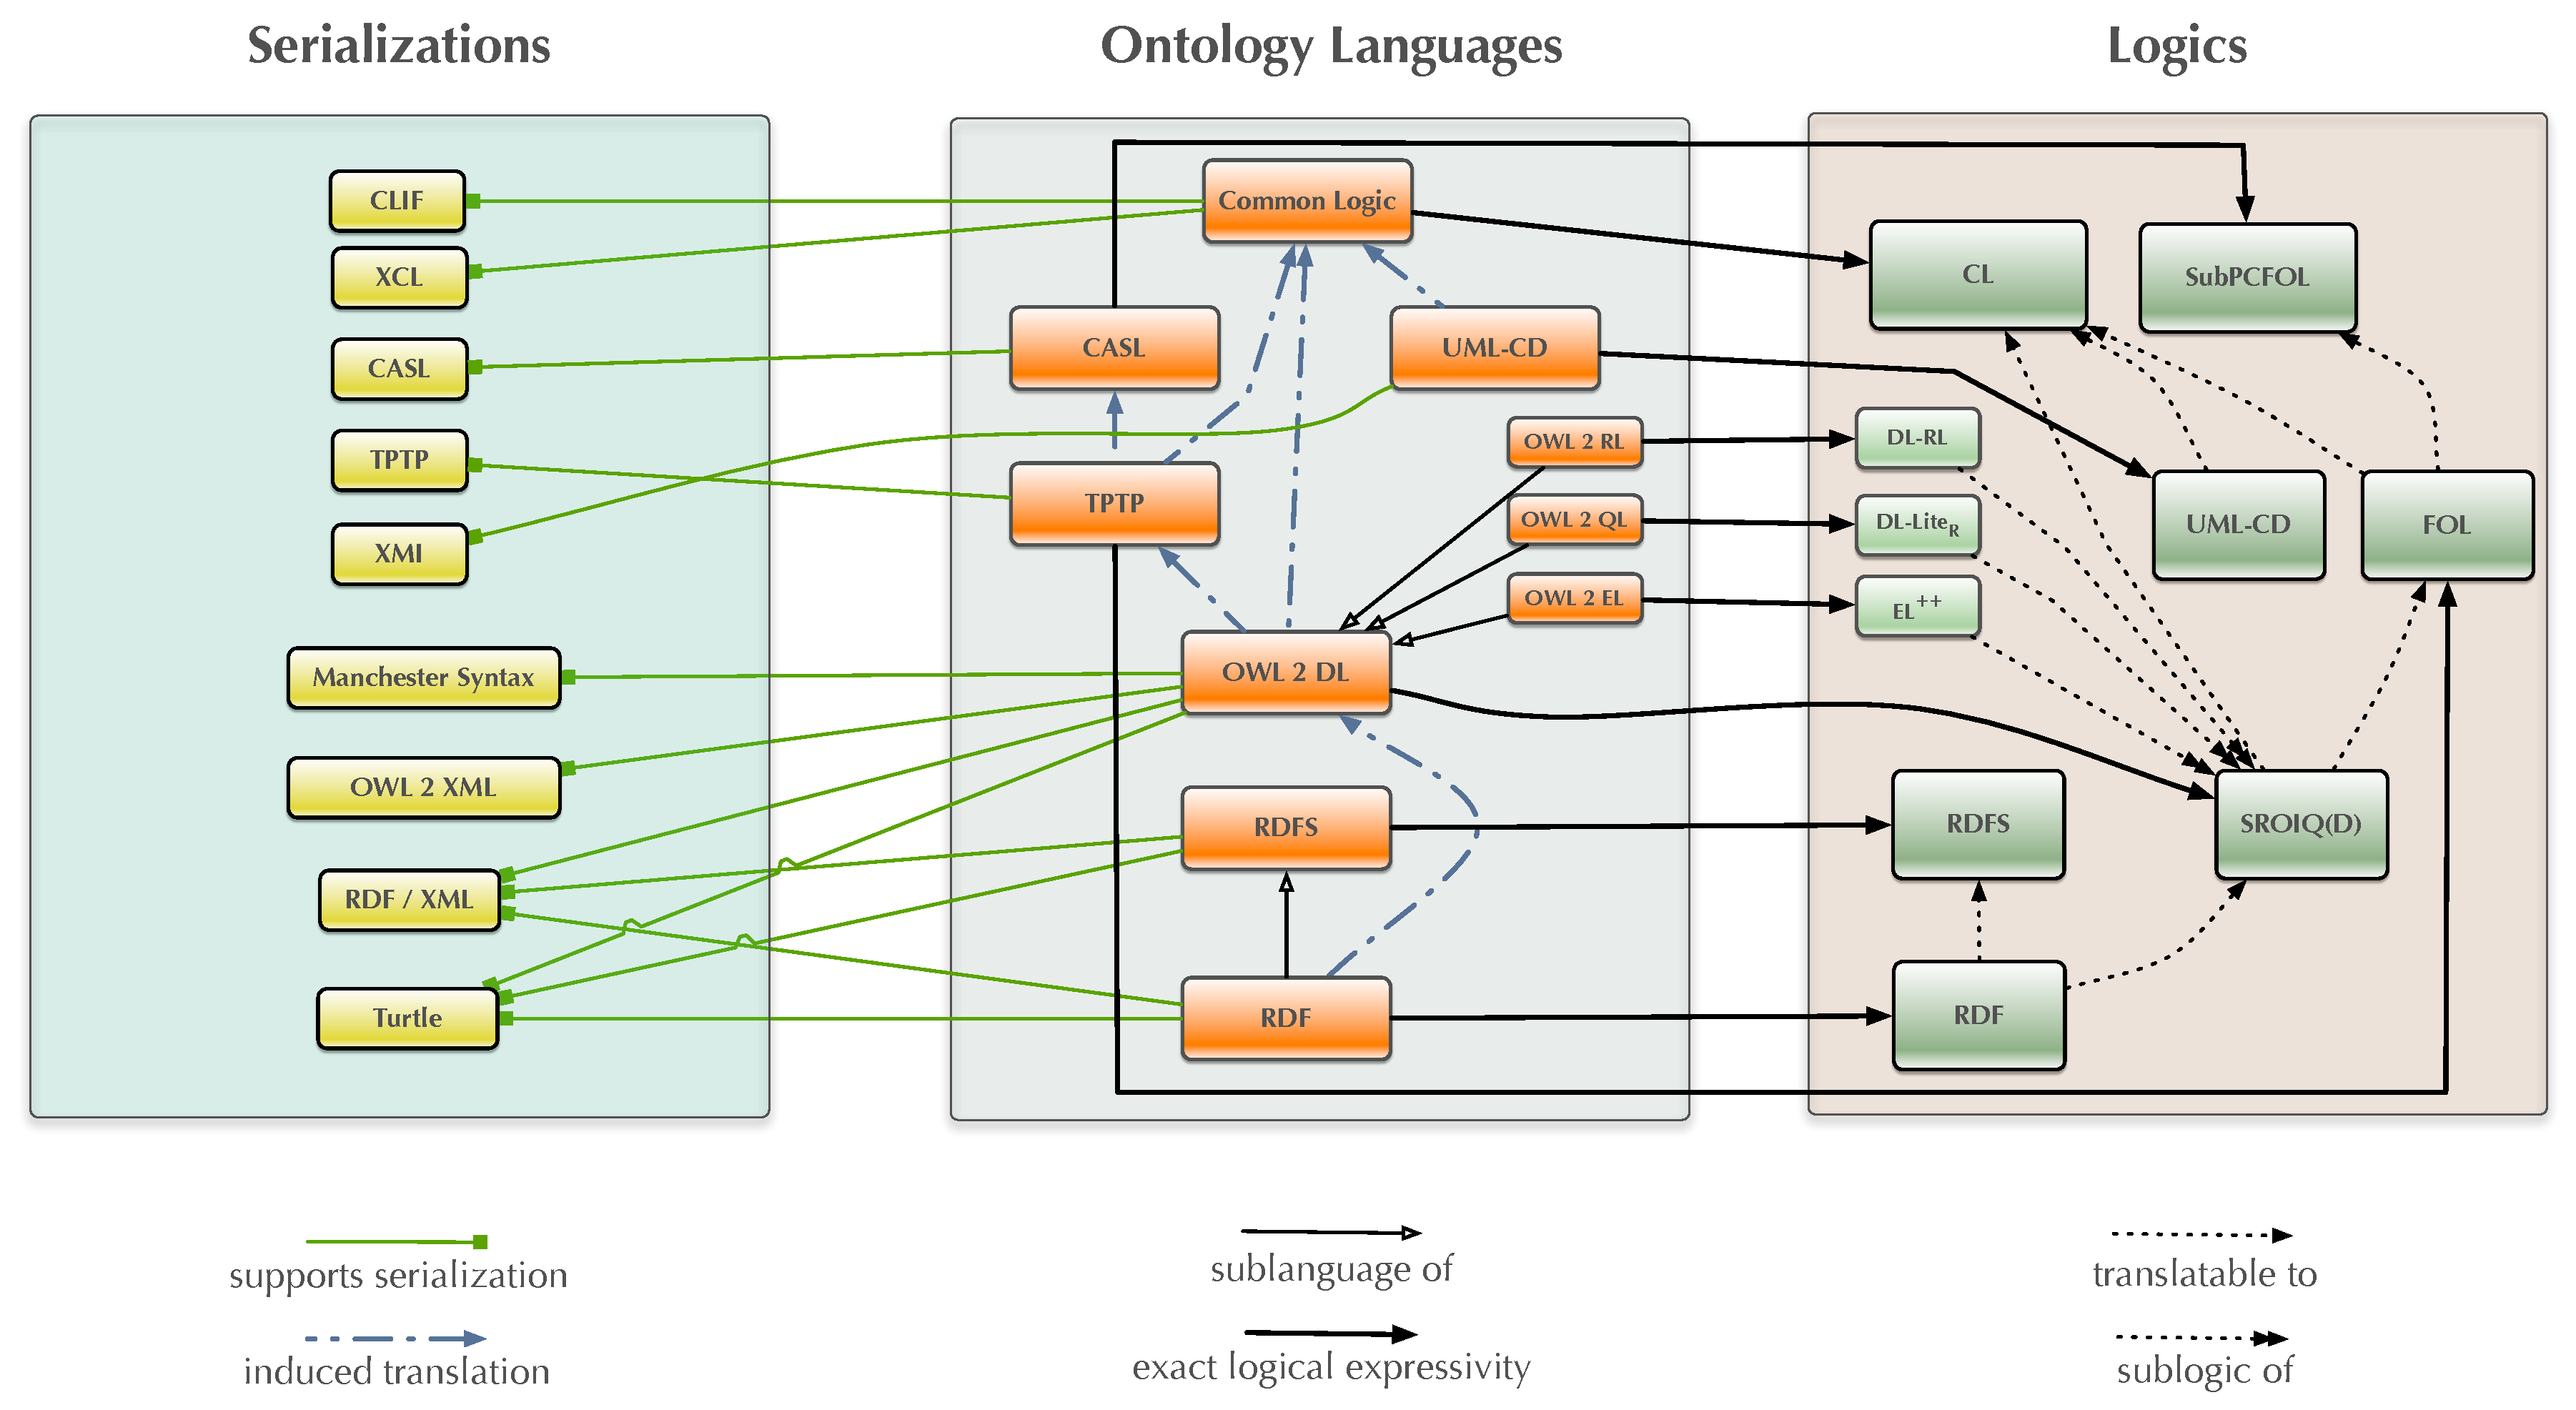
\includegraphics[width=\textwidth]{illustrations/DOL-ontograph-layers-OMG} 
  \caption{Subset of the OntoIOp registry, shown as an RDF graph}
\label{f:DOL-threelayers}
\end{sidewaysfigure}

%\begin{figure}
%  \centering
%   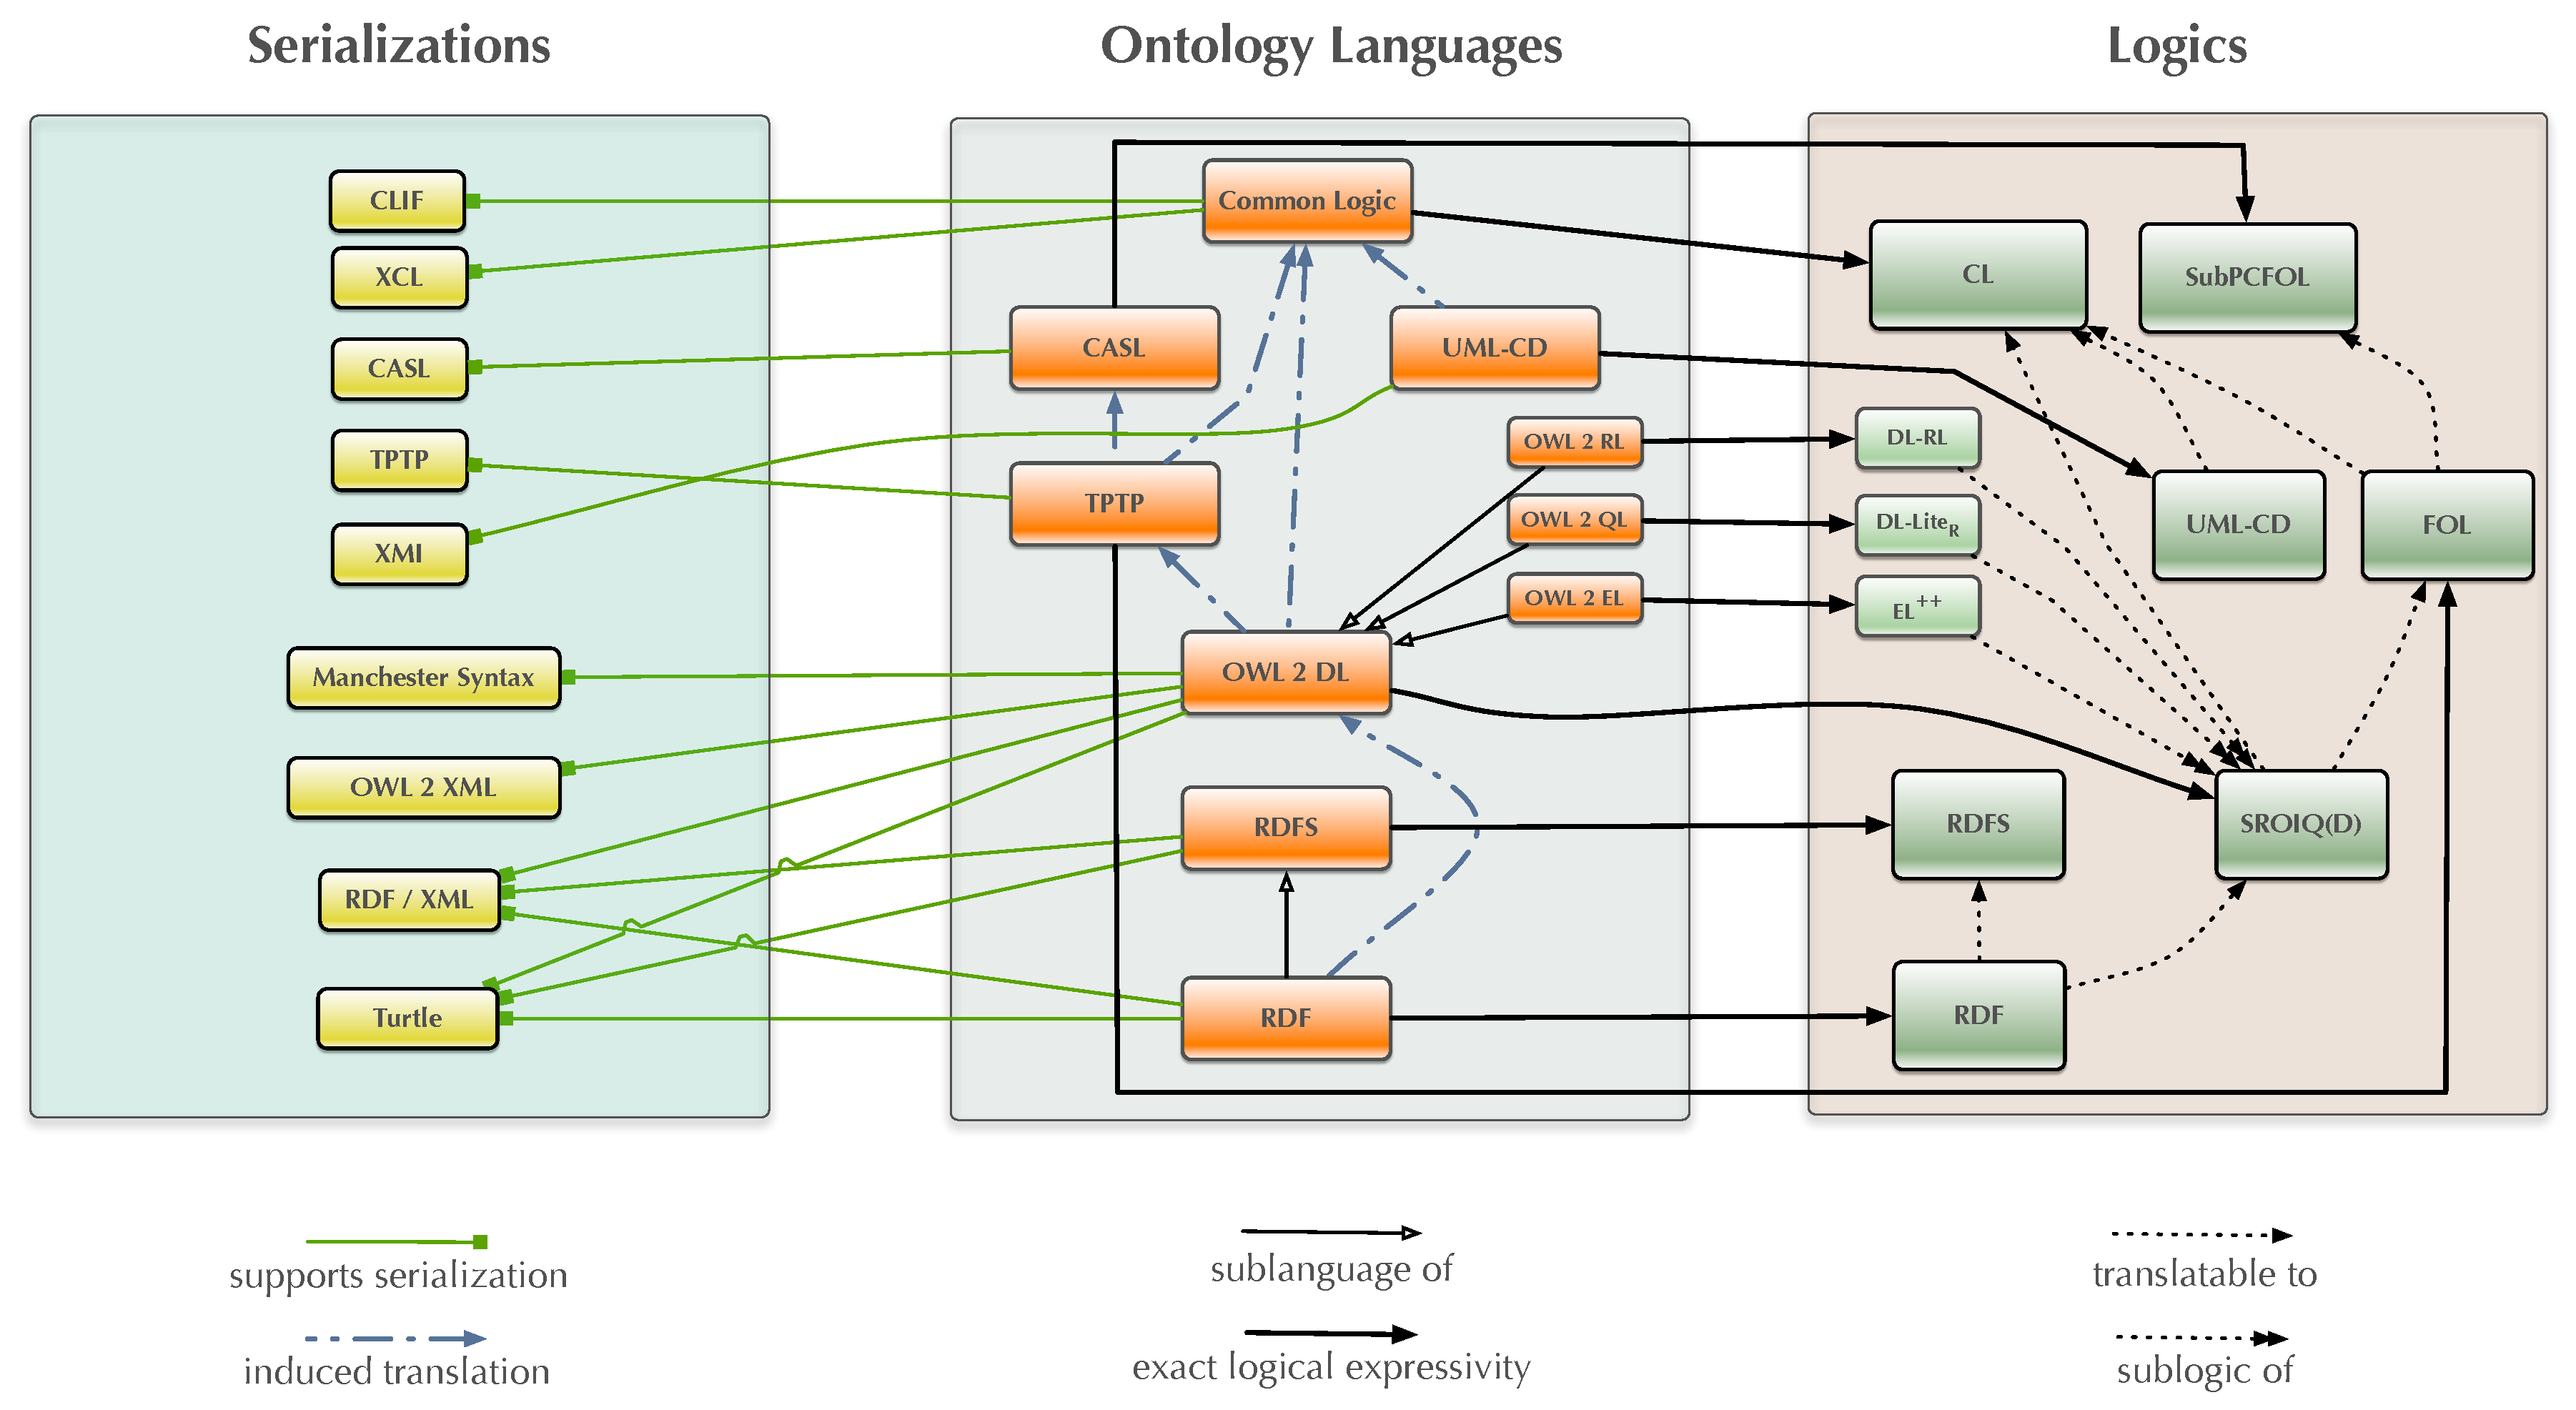
\includegraphics[width=\textwidth]{illustrations/DOL-ontograph-layers-OMG} 
%  \caption{Subset of the OntoIOp registry, shown as an RDF graph}
%\label{f:DOL-threelayers}
%\end{figure}

This annex specifies LoLa, an RDF vocabulary that implements the terms and definitions from \cref{terms-and-defs}.
Applications of LoLa include modeling statements about OMS in RDF, e.g., when annotating OMS, or when describing new conforming logics, OMS languages, serializations, translations, etc., in the \termref{registry} stipulated by chapter~\ref{c:conformance}.
LoLa is currently maintained as an OWL ontology and, prospectively, as an OMS library implemented in \DOL, at \url{https://ontohub.org/meta/lola/ontology}.\footnote{The preferred location for LoLa snapshots being part of this OMG standard is \url{http://www.omg.org/spec/DOL/Current/lola}.}.
For a full treatment of the background and design considerations of LoLa please see~\cite{LMK:LoLaModularOntologyLogLangTrans12}.

The tables in this annex list the classes and object properties of LoLa and thus the essential parts of its implementation.  All classes and object properties are assumed to be in the LoLa namespace unless stated otherwise.

\tref{tab:logic-vocab-classes} lists the classes of LoLa.  Each row of the table translates into the following OWL declarations (given in OWL Manchester syntax~\cite{W3C:NOTE-owl2-manchester-syntax-20091027}).  The definitions of the classes can be found in \cref{terms-and-defs}, sometimes under different names if stated so in the table.  Classes rendered in italics are abstract superclasses that have no direct correspondence in the terminology.

\begin{lstlisting}[language=owl2Manchester]
Class: ...
  SubClassOf: ...
\end{lstlisting}

\newcommand*{\ClassDocumentation}[1]{\textit{#1}}
\ctable[
caption={LoLa Classes},
mincapwidth=\textwidth,
label={tab:logic-vocab-classes},
pos=h,
]{p{.27\textwidth}p{.45\textwidth}p{.22\textwidth}}{% table footnotes
}{\FL
  Class & Superclass & Section \ML
  \textit{Language} & & \NN
  OMSLanguage & \textit{Language} & \ref{c:native-oms} \NN
  Logic & & \ref{c:term-logic} \NN
  Serialization & & \ref{c:term-serializations} \NN
  Mapping & & \ref{c:mappings} (OMS mapping) \NN
  LanguageMapping & Mapping & \NN
  LogicMapping & Mapping & \NN
  Translation & Mapping & \NN
  Reduction & Mapping & \NN
  DefaultMapping & Mapping & \ref{c:terms-features} \NN
  WeaklyExactMapping & Mapping & \ref{s:foundations} \NN
  ExactMapping & WeaklyExactMapping & \ref{s:foundations} \NN
  FaithfulMapping & Mapping & \ref{c:terms-features} \NN
  ModelExpansiveMapping & FaithfulMapping & \ref{c:terms-features} \NN
  ModelBijectiveMapping & ModelExpansiveMapping & \NN
  Embedding & ModelBijectiveMapping, LogicMapping, Translation & \ref{s:foundations} \NN
  PlainMapping & Mapping & \NN
  SimpleTheoroidalMapping & Mapping & \ref{c:term-logic} \LL
}

\tref{tab:logic-vocab-prop} lists the object properties of LoLa.  Each row of the table translates into the following OWL declarations (given in OWL Manchester syntax).  The definitions of the properties can be found in \cref{terms-and-defs}, sometimes under different names if stated so in the table.

\begin{lstlisting}[language=owl2Manchester]
ObjectProperty: ...
  Domain: ...
  Range: ...
  SubPropertyOf: ...
\end{lstlisting}

%\todonote[type=q-aut,author=Christoph Lange]{we need to define ``sublogic'' as a term – how?  I guess that would include the notion of an ``OWL profile''. TM: has been defined in section 4}
% \newcommand*{\PropertyDocumentation}[1]{\NN\multicolumn{3}{p{\linewidth}}{\textit{#1}}}
\ctable[
caption={LoLa Properties},
width=\linewidth,
mincapwidth=\textwidth,
label={tab:logic-vocab-prop},
pos=h,
]{lllX}{% table footnotes
}{\FL
  Property & Domain & Range & Section \ML
  isSubLogicOf & Logic & Logic & \ref{c:term-logic} \NN
  % \PropertyDocumentation{The subject is a sublogic of the object}\ML
  supportsLogic & Language & Logic & \ref{c:term-logic} \NN
  % \PropertyDocumentation{The subject OMS language has a semantics specified in terms of the object logic.}\ML
  specifiesSemanticsOf & Logic & Language & inverse of supportsLogic \NN
  % \PropertyDocumentation{The subject logic is used to specify the semantics of the object OMS language; inverse of supportsLogic.}\ML
  supportsSerialization & Language & Serialization & \ref{c:term-serializations} \NN
  % \PropertyDocumentation{OMS in the subject OMS language can be serialized in the object serialization.  Note that the serialization should be as specific as possible, \ie one should not say that ``OWL can be serialized in XML'' and ``Common Logic can be serialized in XML'', but instead ``OWL can be serialized in OWL/XML'' and ``Common Logic can be serialized in XCL'', taking into account that OWL/XML and XCL are two different XML languages.}\ML
  serializes & Serialization & Language & \ref{c:term-serializations} \NN
  % \PropertyDocumentation{The subject logic is used to specify the semantics of the object OMS language; inverse of supportsSerialization.}\LL
}


\section{DOL Registry}\label{a:registry}

\cbs  \ednote{This paragraph has merely been moved.}
It is expected that \DOL will be used for other languages than the  set of \DOL-conforming
languages that are discussed in this \IS. There is a  \textbf{\termref{registry} for \DOL-conforming languages and translations} hosted
at \url{http://logichub.org}.  The registry  also includes descriptions of
DOL-conforming languages and translations (as well as other information needed by implementors
and users) in both human-readable and machine-processable form.  

There will be Maintenance Authority (MA)\footnote{or, depending on advisability, a Registration
Authority} established to maintain the registry as an informative resource governed by the
standard.  The registry contents itself will not be normative; however, it is 
expected to become the basis for normative activities.
\cbe

\infannex{Conformance of OWL 2 DL With \DOL}\label{a:owl}

The semantic conformance of OWL 2 DL (as specified in \nisref{W3C/TR REC-owl2-syntax:2009}) with \DOL
is established in \cite{OntoGraph}.

The OWL/XML serialization satisfies the criteria for XML conformance.  The mapping of OWL 2 DL to RDF
graphs satisfies the criteria for RDF conformance\CLnote{This is not exactly true, as some things,
e.g. imports, cannot be identified.}.  The OWL 2 Manchester syntax satisfies the criteria for text
 conformance.
%~\CLnote{also need conformance propositional logic; use PL ``profile'' of the CASL ``IFIP standard''}

OWL can be formalized as an institution as follows:
\begin{definition}\label{DL} \defsty{OWL 2 DL.} 
\OWL~2~DL is the description logic (DL) based fragment of the web ontology language \OWL. 
We start with the simple description logic $\ALC$, and then proceed
to the more complex description logic \SROIQ which is underlying \OWL~2~DL.
Signatures of the description logic $\ALC$ consist of a set  ${\mathcal A}$ of
atomic concepts, a set ${\mathcal R}$ of roles and a set ${\mathcal
I}$ of individual constants. Signature morphisms are tuples of
functions, one for each signature component.
Models are  first-order structures $I = (\Delta^I, .^I)$ with universe $\Delta^I$
that interpret concepts as unary and roles as binary predicates
(using $.^I$). $I_1\leq I_2$ if $\Delta^{I_1}=\Delta^{I_2}$ and all
concepts and roles of $I_1$ are subconcepts and subroles of those in $I_2$.
Sentences are subsumption relations $C_1\sqsubseteq C_2$ between
concepts, where concepts follow the grammar
%\CLnote[type=q-aut]{This grammar should also be adapted to ISO EBNF.}
$$C ::= {\mathcal A} \,|\, \top\,|\, \bot \,|\, C_1 \sqcup C_2 \,|\, C_1 \sqcap C_2 \,|\, \neg C 
    \,|\, \forall R . C \,|\, \exists R . C$$
These kind of sentences are also called TBox sentences.
 Sentences can also be ABox sentences, which are
membership assertions of individuals in concepts (written $a:C$ for
$a\in{\mathcal I})$ or pairs of individuals in roles (written $R(a,b)$
for $a,b\in{\mathcal I}, R\in{\mathcal R}$).   Satisfaction is the
standard satisfaction of description logics.

The logic \SROIQ \cite{SROIQ}, which is the logical core of the Web Ontology
Language \OWL 2 DL\footnote{See also \url{http://www.w3.org/TR/owl2-overview/}}, extends $\ALC$
with the following constructs: (i) complex role inclusions such as $R \circ S \sqsubseteq S$
as well as simple role hierarchies such as $R \sqsubseteq S$,
assertions for symmetric, transitive, reflexive, asymmetric and
disjoint roles (called RBox sentences, denoted by $\mathcal{SR}$), as well as the construct
$\exists R . \mathsf{Self}$ (collecting the set of `$R$-reflexive
points'); (ii) nominals, i.e.\ concepts of the form $\{a\}$, where $a\in\mathcal{I}$ (denoted by $\mathcal{O}$); (iii) inverse
roles (denoted by $\mathcal{I}$); qualified and unqualified number
restrictions ($\mathcal{Q}$). For details on the rather complex
grammatical restrictions for \SROIQ (e.g.\ regular role inclusions,
simple roles) compare \cite{SROIQ}.

\OWL \emph{profiles} are syntactic restrictions of \OWL~2~DL that support specific modeling and reasoning tasks, %\cite{w3c:owl2-profiles}, 
and which are accordingly based on DLs with appropriate computational properties. Specifically, \OWL~2~\EL is designed for ontologies containing large numbers of concepts or relations, \OWL~2~\QL to support query answering over large amounts of data, and \OWL~2~\RL to support scalable reasoning using rule languages (\EL, \QL, and \RL for short) .
 
We sketch the logic \ELDL which is underlying the \EL profile.\footnote{To be exact, \EL adds various `harmless' expressive means and syntactic sugar to \ELDL resulting in the DL \ELDL$++$. % \cite{BaaderEtAl-OWLED08DC}; for further details see also \cite{w3c:owl2-profiles}.
} 
\ELDL is a syntactic restriction of \ALC to existential restriction, concept
intersection, and the top concept:
%\ednote{TM@OK: please be  a bit more precise here, perhaps write some grammar: C ::= ⊤ | A | C ⊓ D | ∃r.C, footnote about added sugar in OWL EL profile} Note that \EL is a very relevant ontology language; large medical ontologies like SNOMED\ednote{CL@TM: FYI, it's SNO not SNOW} CT are epxressed in \EL.\ednote{TM@OK: add RL and QL if there is space}
%\ednote{Text entfernt: ``I.e.\ its concepts follow the following grammar'' -- versteht sich IMHO von selbst, nachdem man das obige \ALC-Beispiel gelesen hat}
$$C ::= {\mathcal A} \,|\, \top \,|\,  C_1 \sqcap C_2 \,|\, \exists R . C$$
Note that \ELDL does not have disjunction or negation, and is therefore a sub-Boolean logic.
\qed\end{definition}

Remark: strictly speaking, the institution defined above is
\emph{{OWL} 2 DL without restrictions} in the sense of
\cite{DBLP:conf/owled/SchneiderRS13}. The reason is that in an
institution, the sentences can be used for arbitary formation of
theories. This is related to the presence of \DOL's union operator on
OMS.  OWL 2 DL's specific restrictions on theory formation can be
modeled \emph{inside} this institution, as a constraint on OMS.  This
constraint is generally not preserved under unions or
extensions. \DOL's multi-logic capability allows the clean distinction
between ordinary OWL 2 DL and {OWL} 2 DL without restrictions.


\infannex{Conformance of Common Logic with \DOL}\label{a:cl}

The semantic conformance of Common Logic (as specified in \nisref{ISO/IEC 24707:2007}) with \DOL is established in \cite{OntoGraph}.

The XCF dialect of Common Logic has a serialization that satisfies the criteria for XML conformance.  The CLIF dialect of Common Logic has a serialization that satisfies the criteria for text conformance.

Common Logic can be defined as an institution as follows:

\begin{definition}\label{CommonLogic} \defsty{Common Logic.}  
A common logic signature
$\Sigma$ (called vocabulary in Common Logic terminology) consists of a
set of names, with a subset called the set of discourse names, and a
set of sequence markers. An signature morphism maps
names and sequence markers separately, subject to the requirement
 that a name is a discourse
name in the smaller signature if and only if it is one in the larger signature.  A $\Sigma$-model $I=(\UR,\UD,\rel,\fun,\intCL,\seq)$ consists of a set $\UR$,
the universe of reference, with a non-empty subset $\UD\subseteq \UR$,
the universe of discourse, and four mappings:
  \begin{itemize}
   \item $\rel$ from $\UR$ to subsets of $\UD^* = \{<x_1,\ldots,x_n> |
x_1,\ldots,x_n \in \UD\}$ (i.e., the set of finite sequences of
elements of $\UD$);
   \item $\fun$ from $\UR$ to total functions from $\UD^*$ into $\UD$;
   \item $\intCL$ from names in $\Sigma$ to $\UR$, such that
$\intCL(v)$ is in $\UD$ if and only if $v$ is a discourse name;
   \item $\seq$ from sequence markers in $\Sigma$ to $\UD^*$.
  \end{itemize}  A $\Sigma$-sentence is a first-order
sentence, where predications and function applications are written
in a higher-order like syntax: $t(s)$.
Here, $t$ is an arbitrary term, and $s$ is a sequence term, which can
be a sequence of terms $t_1\ldots t_n$, or a sequence marker.
A predication $t(s)$ is interpreted by evaluating the term $t$,
mapping it to a relation using $\rel$, and then asking whether the sequence
given by the interpretation $s$ is in this relation.  
Similarly, a function application $t(s)$ is interpreted using $\fun$.
Otherwise, interpretation of terms and formulae is as in
first-order logic. 
A further
difference to first-order logic
is the presence of sequence terms (namely sequence markers and
juxtapositions of terms), which denote sequences in $\UD^*$, with term
juxtaposition interpreted by sequence concatenation.
Note that sequences are essentially a non-first-order feature that
can be expressed in second-order logic.

Model reducts are defined in the following way: 
Given a signature morphism $\sigma:\Sigma_1\to\Sigma_2$ and a $\Sigma_2$-model
$I_2=(\UR,\UD,\rel,\fun,\intCL,\seq)$, $I\forget{\sigma}=(\UR,\UD,\rel,\fun,\intCL\circ\sigma,\seq\circ\sigma)$. 

Given two \CL models $I_1=(\UR_1,\UD_1,\rel_1,\fun_1,\intCL_1,\seq_1)$
and  $I_2=(\UR_2,\UD_2,\rel_2,\fun_2,\intCL_2,\seq_2)$, a homomorphism
$h:I_1\to I_2$ is a function $h:\UR_1\to\UR_2$ such that
\begin{itemize}
\item $h$ restricts to $k:\UD_1\to\UD_2$,
\item for each $x\in\UR_1$ and $s\in\UD_1^*$, if $s\in\rel_1(x)$, then $k^*(s)\in\rel_2(h(x))$\footnote{$k^*$ is the extension of $h$ to sequences.},
\item for each $x\in\UR_1$, $k\circ\fun_1(x)=\fun_2(h(x))\circ k^*$,
\item for each name $n$ in $\Sigma$, $\intCL_2(n)=h(\intCL_1(n))$,
\item for each sequence marker $n$ in $\Sigma$, $\seq_2(n)=k^*(\seq_1(n))$.
\end{itemize}

%For details, see \cite{CommonLogic:oldfashioned}.
We call the restriction of \CL to sentence
without sequence markers \CLminus.
\qed\end{definition}

Note that Common Logic also includes sentence formation constructs like
\texttt{cl:import}s that in \DOL terms belong to the structuring
language. They have been omitted from the institution, because
they must not occur in basic OMS. They can occur in
structured native OMS, however, and need to be flattened out
in order to obtain a theory in the \CL institution.
 
\infannex{Conformance of RDF and RDF Schema with \DOL}\label{a:rdfs}

The semantic conformance of RDF Schema (as specified in \nisref{W3C/TR REC-rdf-schema:2014}) with \DOL is established in \cite{OntoGraph}.

The way of representing RDF Schema ontologies as RDF graphs satisfies the criteria for RDF conformance.


\begin{definition}[\RDF and RDF Schema]
Following \cite{Lucanu}, 
we define the institutions for the Resource Description
Framework (\RDF) and \RDF Schema (also known as \RDFS), respectively. 
These are based on a logic called \emph{bare} \RDF (\SimpleRDF), which consists
of triples only (without any predefined resources).

%%%%%%%%%%
A \textit{signature} $\mathbf{R_s}$ in \SimpleRDF is a set of
\textit{resource references}. For $sub, pred, obj \in \mathbf{R_s}$, a
triple of the form $(sub, pred, obj)$ is a \textit{sentence} in \SimpleRDF,
where $sub$, $pred$, $obj$ represent subject name, predicate name,
object name, respectively. An $\mathbf{R_s}$-model $M =
\langle R_m, P_m, S_m, EXT_m \rangle$ consists of a \textit{set $R_m$
  of resources}, a set $P_m \subseteq R_m$ of predicates, a
\textit{mapping function} $S_m:\mathbf{R_s} \rightarrow R_m$, and an
\textit{extension function} $EXT_m: P_m \rightarrow \mathcal{P}(R_m
\times R_m)$ mapping every predicate to a set of pairs of
resources. Satisfaction is defined as follows:
%
\[\mathfrak{M} \models_{\mathbf{R_s}} (sub, pred, obj) \Leftrightarrow (S_{m}(sub),
(S_{m}(obj)) \in EXT_{m} (S_m(pred)). \]
%%%%%
%
Both \RDF and \RDFS are built on top of \SimpleRDF by fixing a certain
standard vocabulary both as part of each signature and in the models.\ednote{Refer to the RDF standard here.}
Actually, the standard vocabulary is given by a certain theory. In case
of \RDF, it contains e.g.\ resources \texttt{rdf:type} and
\texttt{rdf:Property} and \texttt{rdf:subject}, and sentences like, e.g.\
$(\texttt{rdf:type},\texttt{rdf:type},$ $ \texttt{rdf:Property})$, and $(\texttt{rdf:subject}, \texttt{rdf:type},$  $\texttt{rdf:Property})$.

In the models, the standard vocabulary is interpreted with a fixed
model.  Moreover, for each $\RDF$-model $M = \langle R_m, P_m, S_m,
EXT_m \rangle$, if $p\in P_m$, then it must hold
$(p,S_m(\texttt{rdf:Property}))\in EXT_m(\texttt{rdf:type})$.
For \RDFS, similar conditions are formulated (here, for example also
the subclass relation is fixed).


In the case of \RDFS, the standard vocabulary contains more elements,
like
\texttt{rdfs:domain},
\texttt{rdfs:range}, \texttt{rdfs:Resource}, \texttt{rdfs:Literal}, \texttt{rdfs:Datatype}, \texttt{rdfs:Class},
\texttt{rdfs:subClassOf}, \texttt{rdfs:subPropertyOf}, \texttt{rdfs:member}, \texttt{rdfs:Container},
\texttt{rdfs:ContainerMembershipProperty}.

There is also \OWL Full, an extension of \RDFS with resources
such as \texttt{owl:Thing} and \texttt{owl:oneOf}, tailored towards the representation of
\OWL~\cite{W3C:REC-owl2-rdf-based-semantics-20091027}.

\qed\end{definition}


\infannex{Conformance of UML class and object diagrams with \DOL}\label{a:uml-class}

This informative annex demonstrates conformance of UML class and
object diagrams with \DOL by defining an institution for both. We
concentrate on the static aspects of class diagrams; that is, change
of state is ignored. This means that all operations are query
operations.

The institution of UML class and object diagrams is defined using a
translation of UML class diagrams to Common Logic, following the fUML
specification and \cite{Seidewitz08}.

\section{Preliminaries}

From the fUML specification, section 10.3.1, we inherit the axioms for
primitive types: Booleans, numbers, sequences and strings.  These
axiomatize (among others) predicates corresponding to primitive types,
e.g.\ \texttt{buml:Boolean}, \texttt{form:Number},
\texttt{form:NaturalNumber}, \texttt{buml:Integer},
\texttt{form:Sequence}, \texttt{form:Character}, and
\texttt{buml:String}.

We additionally need to axiomatize a number of predicates in Common Logic
(note that enumerations are not axiomatized in fUML):
\begin{lstlisting}[language=clif,morekeywords={then,with,logic,oms,end},mathescape]
logic CLIF

oms pairs =
  (forall (x y) (= (form:first (form:pair x y)) x))
  (forall (x y) (= (form:second (form:pair x y)) y))
  (forall (x y) (form:Pair (form:pair x y)))
  (forall (p) (if (form:Pair p)
                  (= (form:pair (form:first p) (form:second p)) p)))
end

oms sequences =
fuml:sequences.clif and pairs
then
  // fuml:sequence - membership of an element in a sequence
  (forall (x s)
      (if (form:sequence-member x s)
          (form:Sequence s)))

  (forall (x s)
      (iff (form:sequence-member x s)
           (exists (pt) 
               (and (form:in-sequence s pt)
                    (form:in-position pt x)) )))

  // selection of elements
  (forall (o) (= (form:select1 o form:empty-sequence) form:empty-sequence))
  (forall (o y s)
          (= (form:select1 o (form:sequence-insert (form:pair o y) s)) 
             (form:sequence-insert y (form:select1 o s))))
  (forall (o x y s)
          (if (not (= x o))
              (= (form:select1 o (form:sequence-insert (form:pair x y) s)) 
                 (form:select1 o s))))
  (forall (o) (= (form:select2 o form:empty-sequence) form:empty-sequence))
  (forall (o x s)
          (= (form:select2 o (form:sequence-insert (form:pair x o) s)) 
             (form:sequence-insert x (form:select2 o s))))
  (forall (o x y s)
          (if (not (= y o))
              (= (form:select2 o (form:sequence-insert (form:pair x y) s)) 
                 (form:select2 o s))))

  (forall (i s)
          (= (form:n-select form:empty-sequence i s) 
             form:empty-sequence))
  (forall (a i s t x)
          (if (= (insert-i i x t) s)
              (= (form:n-select (form:sequence-insert s a) i t)
                 (form:sequence-insert s (form:n-select a i t)))))
  (forall (a i s t)
          (if (not (exists (x) (= (insert-i i x t) s)))
              (= (form:n-select (form:sequence-insert s a) i t)
                 (form:n-select a i t))))

  // insert element at i-th position
  (forall (x s)
          (= (insert-i form:0 x s) (form:sequence-insert x s)))
  (forall (i j x y s)
          (if (form:add-one i j)
              (= (insert-i j x (form:sequence-insert y s))
                 (form:sequence-insert y (insert-i i x s)))))
end

oms sequences-insert =
sequences then
  // insertion of elements
  (forall (x s1 s2)
    // inserting an element means...
    (if (= (form:sequence-insert x s1) s2)
        (and (form:Sequence s1)
             (form:Sequence s2)
             // the new element is at the first position
             (form:in-position-count s2 form:1 x)
             // and all other elements are shifted by one
             (forall (n1 n2 y)
               (if (form:add-one n1 n2)
                   (iff (form:in-position-count s1 n1 y)
                        (form:in-position-count s2 n2 y)))))))
  // synonym
 (forall (s) (= (form:sequence-length s) (form:sequence-size s)))
end

oms ordered-sets =
sequences with
  form:Sequence |-> form:Ordered-Set,
  form:empty-sequence |-> form:empty-ordered-set,
  form:sequence-length |-> form:ordered-set-size,
  form:same-sequence |-> form:same-ordered-set,
  form:sequence-member |-> form:ordered-set-member,
  form:in-sequence |-> form:in-ordered-set,
  form:before-in-sequence |-> form:before-in-ordered-set,
  form:position-count |-> form:ordered-set-position-count
  form:in-position-count |-> form:in-ordered-set-position-count
then
//Different positions contain different elements
  (forall (s x1 x2 n1 n2)
  	    (if (and (form:in-ordered-set-position-count s n1 x1)
  	  	     (form:in-ordered-set-position-count s n2 x2)
                     (= x1 x2))
                (= n1 n2)))
  // insertion of elements
  (forall (x s1 s2)
    (if (= (form:ordered-set-insert x s1) s2)
        (and (form:Ordererd-Set s1)
             (form:Ordererd-Set s2)
  // no element can be inserted twice
  (forall (x s)
    (if (from:ordered-set-member x s)
        (= (form:ordered-set-insert x s) s)))
  // inserting a new element
  (forall (x s)
    (if (not (from:ordered-set-member x s1))
        (exists (s2)
          (and (= (form:ordered-set-insert x s1) s2)     
               // the new element is at the first position
               (form:in-ordered-set-position-count s2 form:1 x)
               // and all other elements are shifted by one
               (forall (n1 n2 y)
                 (if (form:add-one n1 n2)
                     (iff (form:in-ordered-set-position-count s1 n1 y)
                          (form:in-ordered-set-position-count s2 n2 y)))))))
end

oms sets =
//An empty set has no members.
(forall (s)
	(if (form:empty-set s)
	    (form:Set s)))
(forall (s)
	(if (form:Set s)
	    (iff (form:empty-set s)
		 (not (exists (x)
			      (form:set-member x s))))))
//Size of sets
(forall (s n)
	(if (form:set-size s n)
	    (and (form:Set s)
		 (buml:UnlimitedNatural n))))
(= (form:set-size form:empty-set) form:0)
(forall (x s)
        (if (not (form:set-member x s))
            (exists (n)
              (and (form:add-one (form:set-size s) n)
                   (= (form:set-size (form:set-insert x s))
                      n)))))

//The same-set relation is true for sets that have the same members.
// but: why not replace same-set with = ?
(forall (s1 s2)
	(if (form:same-set s1 s2)
	    (and (form:Set s1)
		 (form:Set s2))))
(forall (s1 s2)
	(iff (form:same-set s1 s2)
	     (forall (x)
		     (iff (form:set-member x s1)
			  (form:set-member x s2)))))
//Insertion of elements into sets and set membership
(forall (x s)
	(if (form:Set s)
	    (form:Set (form:set-insert x s))))
(forall (x y s)
        (iff (form:set-member x (form:set-insert y s))
             (or (= x y)
                 (form:set-member x s))))
end

oms bags =
//An empty bag has no members.
(forall (s)
	(if (form:empty-bag s)
	    (form:Bag s)))
(forall (s)
	(if (form:Bag s)
	    (iff (form:empty-bag s)
		 (not (exists (x)
			      (form:bag-member x s))))))
//Size of bags
(forall (s n)
	(if (form:bag-size s n)
	    (and (form:Bag s)
		 (buml:UnlimitedNatural n))))
(= (form:bag-size form:empty-bag) form:0)
(forall (x s)
        (exists (n)
            (and (form:add-one (form:bag-size s) n)
                 (= (form:bag-size (form:bag-insert x s))
                    n))))

//The same-bag relation is true for bags that have the same members.
(forall (s1 s2)
	(if (form:same-bag s1 s2)
	    (and (form:Bag s1)
		 (form:Bag s2))))
(forall (s1 s2)
	(iff (form:same-bag s1 s2)
	     (forall (x)
		     (iff (form:bag-member-count x s1)
			  (form:bag-member-count x s2)))))
//Insertion of elements into bags and bag membership
(forall (x s)
	(if (form:Bag s)
	    (form:Bag (form:bag-insert x s))))
(forall (x y s)
        (iff (form:bag-member x (form:bag-insert y s))
             (or (= x y)
                 (form:bag-member x s))))
//Member count
(forall (x s)
	(if (form:Bag s)
	    (buml:UnlimitedNatural (form:bag-member-count x s))))
(= (form:bag-member-count form:empty-bag) form:0)
(forall (x s)
        (exists (n)
           (and (form:add-one (form:bag-member-count x s) n)
                (= (form:bag-member-count x (form:bag-insert x s))
                   n))))
(forall (x y s)
        (if (not (= x y))
            (= (form:bag-member-count x (form:bag-insert y s))
               (form:bag-member-count x s))))
end

oms collection-types =
  sequences-insert and ordered-sets and sets and bags
then
//bag to set
(forall (b)
	(if (form:Bag s)
	    (form:Set (form:bag2set b))))
(= (form:bag2set form:empty-bag) form:empty-set)
(forall (x b)
        (if (form:Bag b)
            (= (form:bag2set (form:set-insert x b))
               (form:bag-insert x (form:bag2set b)))))

//sequence to ordered set
(forall (s)
	(if (form:Sequence s)
	    (form:Ordered-Set (form:seq2ordset s))))
(= (form:seq2ordset form:empty-sequence) form:empty-ordered-set)
(forall (x s)
        (if (form:Sequence s)
            (= (form:seq2ordset (form:sequence-insert x s))
               (form:ordered-set-insert x (form:seq2ordset s)))))

//sequence to bag
(forall (s)
	(if (form:Sequence s)
	    (form:Bag (form:seq2bag s))))
(= (form:seq2bag form:empty-sequence) form:empty-bag)
(forall (x s)
        (if (form:Sequence s)
            (= (form:seq2bag (form:sequence-insert x s))
               (form:bag-insert x (form:seq2bag s)))))

//ordered-set to set
(forall (b)
	(if (form:Ordered-Set s)
	    (form:Set (form:ordset2set b))))
(= (form:ordset2set form:empty-ordered-set) form:empty-set)
(forall (x b)
        (if (form:Ordered-Set b)
            (= (form:ordset2set (form:set-insert x b))
               (form:ordered-set-insert x (form:ordset2set b)))))

//sequence to set
(forall (s)
	(if (form:Sequence s)
	    (form:Set (form:seq2set s))))
(forall (s) (= (form:seq2set s) (form:ordset2set (form:seq2ordset s))))

// leq
(forall (x y)
   (iff (buml:leq x y)
        (or (= x y)
            (buml:less-than x y))))
end


oms uml-cd-preliminaries =
  collection-types and pairs
end

\end{lstlisting}

Using this infrastructure, we obtain an institution for UML class
diagrams as described in the following sections.

\section{Signatures}

\medskip\noindent\textbf{Class/data type hierarchies.}  A
\emph{class/data type hierarchy} $(C, {\leq_C})$ is given by a partial
order where the set $C$ contains the \emph{class/data type names}, which
are closed w.r.t.\ the \emph{built-in data types} $\mathsf{Boolean}$,
$\mathsf{UnlimitedNatural}$, $\mathsf{Integer}$, $\mathsf{Real}$, and
$\mathsf{String}$, i.e.,
$\{ \mathsf{Boolean}, \mathsf{UnlimitedNatural},\allowbreak
\mathsf{Integer}, \mathsf{Real}, \mathsf{String} \} \subseteq
C$;
%\ednote{what
%  about enumeration types? Should we assume that some classifiers are
%  marked as enumeration types and equipped with their set of constants?
%  AK: In UML, \uml{Enumeration} is a specialisation of \uml{DataType}.
%  The set of constants are \uml{EnumerationLiteral}s.  These could be
%  added like \uml{Property}.}
and the partial ordering relation $\leq_C$ represents a
\emph{generalisation relation} on $C$, where we say that $c_1$ is a
\emph{sub-class/data type} of $c_2$ if $c_1 \leq_C c_2$.

A \emph{class/data type hierarchy map}
$\gamma : (C, {\leq_C}) \to (D, {\leq_D})$ is given by a monotone map
from $(C, {\leq_C})$ to $(D, {\leq_D})$, i.e.,
$\gamma(c) \leq_D \gamma(c')$ if $c \leq_C c'$, such that
$\gamma(c) = c$ for all
$c \in \{ \mathsf{Boolean},\allowbreak \mathsf{UnlimitedNatural},\allowbreak
\mathsf{Integer}, \mathsf{Real}, \mathsf{String} \}$.

\medskip
We use the \emph{collection type constructors} $\mathsf{OrderedSet}$,
$\mathsf{Set}$, $\mathsf{Sequence}$, and $\mathsf{Bag}$ for
representing the meta-attributes ``ordered'' and ``unique'' of
\uml{MultiplicityElement} according to the following
table:\footnote{Cf.~UML Superstructure Specification 2.4.1, p.~128; UML
  2.5, p.~27.}
%
\begin{quotation}
\begin{tabular}{@{}r||c|c@{}}
             & ordered               & not ordered\\
\hline\hline
  unique     & $\mathsf{OrderedSet}$ & $\mathsf{Set}$\\
\hline
  not unique & $\mathsf{Sequence}$   & $\mathsf{Bag}$
\end{tabular}
\end{quotation}
%
The default is ``not ordered'' and ``unique''.\footnote{UML
  Superstructure Specification 2.4.1, p.~96; there does not seem to be
  default in UML 2.5.}

For a class/data type $c \in C$ of a class/data type-hierarchy
$(C, {\leq_C})$ and a collection type constructor
$\tau \in \{ \mathsf{OrderedSet}, \mathsf{Set}, \mathsf{Sequence},
\mathsf{Bag} \}$,
we write $\tau[c]$ for the induced \emph{collection type}.

\medskip
Let $(C, {\leq_C})$ be a class/data type hierarchy.
%
\begin{itemize}[label={--}, leftmargin=*]
  \item An \emph{attribute declaration}\footnote{We separate attributes
  from association member ends due to their different uses.  In UML,
  both are of class \uml{Property}.} over $(C, {\leq_C})$ is of the form
$c.p : \tau[c']$ with $c, c' \in C$, $\tau$ a collection type
constructor, and $p$ an \emph{attribute name}.

  \item A \emph{query operation declaration} over $(C, {\leq_C})$ is of
the form $c.q(x_1 : \tau_1[c_1], \dots, x_r : \tau_r[c_r]) : \tau[c']$
with $c, c_1,\ldots, c_r, c' \in C$, $\tau$ a collection type
constructor, $o$ an \emph{operation name}, and $x_1, \ldots, x_r$
\emph{parameter names}.

\item An \emph{association declaration} over $(C, {\leq_C})$ is of the
form $a(p_1 : \tau_1[c_1], \dots, p_r : \tau_r[c_r])$ with $r \geq 2$,
$c_1, \dots, c_r \in C$, $\tau_1, \ldots, \tau_r$ classifier
annotations, $a$ an \emph{association name}, and $p_1, \dots, p_r$
\emph{member end names}.\footnote{The member ends are ordered according
  to the UML Superstructure Specification 2.4.1, p.~29; UML 2.5, p.~206;
  hence we use a tuple-like notation.}  An association declaration
$\mathbf{a} = a(p_1 : \tau_1[c_1], \ldots, p_r : \tau_r[c_r])$
\emph{yields} the \emph{property declarations}
$\mathbf{a}.p_i : \tau_i[c_i]$ for $1 \leq i \leq r$.  An association
declaration is \emph{binary} if $r = 2$.\footnote{Only binary
  association may show member ends that are properties not owned by the
  association (UML Superstructure Specification 2.4.1, p.~37; UML 2.5,
  p.~228).  The propery declarations induced by a more than binary
  association result in a query operation.}

  \item A \emph{composition declaration} over $(C, {\leq_C})$ is of the
form $m(p_1 : \mathsf{Set}[c_1], \composition p_2 : \tau_2[c_2])$ with
$c_1, c_2 \in C$, $\tau_2$ a collection type constructor, $m$ a
\emph{composition name}, and $p_1, p_2$ \emph{member end
  names}.\footnote{In UML, each \uml{Property} may have
  \uml{AggregationKind} \uml{composite}.  However, such an aggregation
  kind has no semantic meaning when the property is not a member end of
  an association: the UML Superstructure Specification 2.4.1 does not
  mention the aggregation kind in the description of the semantics of
  \uml{Property}, and UML 2.5 explains the use of aggregations for
  \uml{Property} as ``to model circumstances in which \emph{one
    instance} is used to group together a set of instances'' (p.~112,
  our emphasis).  Moreover, composite properties, i.e., properties with
  aggregation kind \uml{composite} can only be member ends of binary
  associations (UML Superstructure Specification 2.4.1, p.~37; UML 2.5,
  p.~228) and their multiplicity must not exceed one (UML Superstructure
  Specification 2.4.1, p.~126; UML 2.5, p.~155).  We thus separate
  composition declarations from general association declarations.}  A
composition declaration
$\mathbf{m} = m(p_1 : \mathsf{Set}[c_1], \composition p_2 :
\tau_2[c_2])$
\emph{yields} the property declarations
$\mathbf{m}.p_1 : \mathsf{Set}[c_1]$ and $\mathbf{m}.p_2 : \tau_2[c_2]$.
\end{itemize}

\medskip\noindent\textbf{Class/data type nets (Signatures).}
A \emph{class/data type net} $\Sigma = ((C, {\leq_C}), P, O, A, M)$
comprises a class/data type hierarchy $(C, {\leq_C})$ and a set $P$ of
attribute declarations, a set $O$ of operation declarations,
 a set $A$ of association declarations over
$(C, {\leq_C})$, and a set $M$ of composition declarations over $(C, {\leq_C})$, such that
the following properties are satisfied:
%
\begin{itemize}[label={--}, leftmargin=*]
  \item attribute names are unique along the generalisation relation: if
$c_1.p_1 : \tau_1[c_1']$ and $c_2.p_2 : \tau_2[c_2']$ are different
property declararations in $P$ and $c_1 \leq_C c_2$, then $p_1 \neq
p_2$;

  \item association and composition names are unique: if $d_1$ and
$d_2$ are the names of two different association or composition
declarations in $M \cup A$, then $d_1 \neq d_2$;

  \item member end names are unique: if $p_1, \ldots, p_r$ are the
member end names of an association declaration in $A$ or a composition
declaration in $M$, then $p_i \neq p_j$ for
$1 \leq i \neq j \leq r$;\footnote{In UML, member end names need not be
  unique.  However, for (1)~a simpler handling of selecting a particular
  member end in the sentences and avoiding the use of number selectors,
  and (2)~making the notion of member ends ``owned'' by a class/data
  type, we add this constraint. An association declaration violating this
  uniqueness constraints can easily be transformed into an association 
  declaration satisfying it by decorating member end names with the
  numbers $1,\ldots,r$.}

  \item the type of a member end\footnote{All member ends are instances
  of \uml{Property}; UML Superstructure Specification 2.4.1, p.~36; UML
  2.5, p.~206.}
owned by a class/data type coincides with its declarations as attribute:
We say that a property declaration $\mathbf{a}.p_i : \tau_i[c_i]$
yielded by a binary association
$\mathbf{a} = a(p_1 : \tau_1[c_1], p_2 : \tau_2[c_2])$ is \emph{owned
  by} $c_0 \in C$ if $c_{3-i} \leq_C c_0$ and there is an attribute
declaration $c_0.p_i : \tau_i[c_i] \in P$; and similarly for property
declarations yielded by composition declarations.  (Note that by the
uniqueness of attribute names along the generalisation hierarchy only a
single attribute with name $p_i$ may exist.)
\end{itemize}

A \emph{class/data type net morphism}
$\sigma = (\gamma, \varphi, \alpha, \mu) : \Sigma = ((C,
{\leq}_C), P, A, M) \to \Tau = ((D, {\leq}_D),\allowbreak
Q,\allowbreak B, N)$ is given by
%
\begin{itemize}[label={--}, leftmargin=*]
  \item a class/data type hierarchy map $\gamma : (C, {\leq_C}) \to (D,
{\leq_D})$;

  \item an attribute declaration map $\varphi : P \to Q$ such that if
$\varphi({c.p : \tau[c']}) = {d.q : \tau'[d']} \in Q$, then
$d = \gamma(c)$, $d' = \gamma(c')$, and $\tau = \tau'$;

  \item a query operation declaration map $\rho : O \to R$ such that if
$\rho(c.q(x_1 : \tau_1[c_1], \dots, x_r : \tau_r[c_r]) : \tau[c']) =
d.r(x_1 : \tau'_1[d_1], \dots, x_r : \tau'_r[d_r]) : \tau[d'] \in R$, 
then $d = \gamma(c)$, $d_i = \gamma(c_i)$, 
$d' = \gamma(c')$, $\tau'_i = \tau_i$ and $\tau = \tau'$;

  \item an association declaration map $\alpha : A \to B$ such that if
$\alpha(a(p_1 : \tau_1[c_1], \dots, p_r : \tau_r[c_r])) = b(q_1 :
\tau_1'[d_1], \dots, q_s : \tau_s'[d_s]) \in B$,
then $r = s$ and $d_i = \gamma(c_i)$ and $\tau_i = \tau_i'$ for
$1 \leq i \leq r$, and member ends owned by the association are mapped
into owned member ends;

  \item a composition declaration map $\mu : M \to N$ such that if
$\mu(m(p_1 : \mathsf{Set}[c_1], \composition p_2 : \tau_2[c_2])) =
n(q_1 : \mathsf{Set}[d_1], \composition q_2 : \tau_2'[d_2]) \in N$,
then $d_1 = \gamma(c_1)$, $d_2 = \gamma(c_2)$, and $\tau_2 = \tau_2'$,
and member ends owned by the composition are mapped into owned member
ends.
\end{itemize}

Class/data type nets as objects and class/data type net morphisms as
morphisms form the category of \emph{class/data type nets}, denoted by
$\mathrm{Cl}$.

\medskip
For the example in Fig. \ref{fig:bjoerners_dsl} we have
%
\begin{gather*}
  \text{Classes/data types: }\mathsf{Net}, \mathsf{Station}, \mathsf{Line}, \mathsf{Connector}, \mathsf{Unit}, \mathsf{Track}, \mathsf{Point}, \mathsf{Linear},
\\[-.5ex]
  \phantom{\text{Classes/data types: }}\mathsf{Boolean}, \mathsf{UnlimitedNatural}, \mathsf{Integer}, \mathsf{Real}, \mathsf{String}
\\
  \text{Generalisations: }\mathsf{Point} \leq \mathsf{Unit}, \mathsf{Linear} \leq \mathsf{Unit}
\\
  \text{Properties: }\mathsf{Line.linear : Set[Boolean]}, \mathsf{Track.linear : Set[Boolean]},
\\[-.5ex]
  \phantom{\text{Properties: }}\mathsf{Net.station : Set[Station]}, \mathsf{Net.line : Set[Line]},
\\[-.5ex]
  \phantom{\text{Properties: }}\mathsf{Station.net : Set[Net]}, \mathsf{Station.unit : Set[Unit]}, \mathsf{Station.track : Set[Track]},
\\[-.5ex]
  \phantom{\text{Properties: }}\mathsf{Line.net : Set[Net]}, \mathsf{Line.linear : Set[Linear]},
\\[-.5ex]
  \phantom{\text{Properties: }}\mathsf{Connector.unit : Set[Unit]},
\\[-.5ex]
  \phantom{\text{Properties: }}\mathsf{Unit.station : Set[Station]}, \mathsf{Unit.connector : Set[Connector]},
\\[-.5ex]
  \phantom{\text{Properties: }}\mathsf{Track.station : Set[Station]}, \mathsf{Track.linear : Set[Linear]},
\\[-.5ex]
  \phantom{\text{Properties: }}\mathsf{Linear.track : Set[Track]}, \mathsf{Linear.line : Set[Line]}
\\
  \text{Associations: }\mathsf{l2l(line : Set[Line], linear : Set[Linear])},
\\[-.5ex]
  \phantom{\text{Associations: }}\mathsf{l2t(linear : Set[Linear], track : Set[Track])},
\\[-.5ex]
  \phantom{\text{Associations: }}\mathsf{c2u(connector : Set[Connector], unit : Set[Unit])}
\\
  \text{Compositions: }\mathsf{n2s(net : Set[Net], \composition station : Set[Station])},
\\[-.5ex]
  \phantom{\text{Compositions: }}\mathsf{n2l(net : Set[Net], \composition line : Set[Line])},
\\[-.5ex]
  \phantom{\text{Compositions: }}\mathsf{s2u(station : Set[Station], \composition unit : Set[Unit])},
\\[-.5ex]
  \phantom{\text{Compositions: }}\mathsf{s2t(station : Set[Station], \composition track : Set[Track])}
\end{gather*}
%
Here all member ends are owned by class/data types.


\begin{figure}[!tH]
\begin{center}
\vspace*{1ex}
\begin{tikzpicture}[transform shape,scale=.8]
\def\overallfont{\sffamily\fontsize{10pt}{10pt}\selectfont}
\tikzset{every node/.style={font=\overallfont}}
%\tikzset{tikzuml class style/.style={inner xsep=32pt}}
\tikzumlset{font=\overallfont}
\umlemptyclass{Net}
\umlemptyclass[x=-2, y=-3]{Station}
\umlclass[x=2.5, y=-3]{Line}{linear : Boolean}{}
\umlcompo[name=NetStation,mult2=2..*, pos2=2.7, geometry=|-|]{Net}{Station}
\draw (NetStation-4) node[above] {n2s};
\umlcompo[name=NetLine,mult1=1, pos1=0.3, mult2=*, pos2=2.7, geometry=|-|]{Net}{Line}
\draw (NetLine-4) node[above] {n2l};
\umlemptyclass[x=-4, y=-6]{Unit}
\umlclass[x=0, y=-6]{Track}{linear : Boolean}{}
\umlcompo[name=StationUnit,mult2=*, pos2=2.7, geometry=|-|]{Station}{Unit}
\draw (StationUnit-4) node[above] {s2u};
\umlcompo[name=StationTrack,mult1=1, pos1=0.3, mult2=*, pos2=2.7, geometry=|-|]{Station}{Track}
\draw (StationTrack-4) node[above] {s2t};
\umlemptyclass[x=-8, y=-6]{Connector}
\umlassoc[name=ConnectorUnit, mult1=1..4, pos1=0, align1=left, mult2=1, pos2=1, align2=right]{Connector}{Unit}
\draw (ConnectorUnit-middle) node[above] {c2u};
\umlemptyclass[x=-6, y=-9]{Point}
\umlemptyclass[x=-2, y=-9]{Linear}
\umlinherit[geometry=|-|]{Point}{Unit}
\umlinherit[geometry=|-|]{Linear}{Unit}
\umlassoc[name=LinearTrack, mult1=1..*, pos1=0, align1=left, anchor1=20, mult2=1, pos2=2, align2=left, geometry=-|]{Linear}{Track}
\draw (LinearTrack-2) node[right] {l2t};
\umlassoc[name=LinearLine, mult1=1..*, pos1=0, align1=left, anchor1=-20, mult2=1, pos2=2, align2=left, geometry=-|]{Linear}{Line}
\draw (LinearLine-2) node[right] {l2l};
\end{tikzpicture}
\end{center}
\caption{Sample UML class diagram.}
\label{fig:bjoerners_dsl}
\end{figure}

\section{Models}\label{a:UML-CD-models}

As stated above, models (in the sense of the term \termref{model} defined in
clause~\ref{terms-and-defs}) of UML class diagrams are obtained 
via a translation to Common Logic.

For a classifier net
$\Sigma = ((C, {\leq_C}), K, P, M, A)$, we define a Common Logic theory
$CL(\Sigma)$ consisting of:
%
\begin{itemize} % [topsep=0pt, label=--, leftmargin=*]
\item for $c \in C$, a predicate\footnote{Strictly speaking, this is just a name.} $\CL(c)$,  such that
%\ednote{class predicates should be restricted to be unary} 
\begin{itemize} % [topsep=0pt, label=--, leftmargin=*]
\item 
  $\CL(\mathsf{Boolean}) = \texttt{buml:Boolean}$, 
\item 
  $\CL(\mathsf{String}) = \texttt{buml:String}$,
\item 
  $\CL(\mathsf{Integer}) = \texttt{buml:Integer}$,
\item 
  $\CL(\mathsf{UnlimitedNatural}) = \texttt{form:NaturalNumber}$,
\item 
  $\CL(\mathsf{Real}) = \texttt{buml:Real}$,
\item 
  $\CL(\mathsf{c}) = c$, if $c$ is an enumeration type with values $k_1,\ldots,k_n$. In this case, additionally, the Common Logic theory is augmented by
\texttt{(not (= $k_i$ $\cdots$ $k_j$))} for $i\neq j$ and
\texttt{(forall (x) (if (c x) (or (= x $k_1$) $\cdots$ (= x $k_n$))))},
%\ednote{Ed Seidewitz:
%enumerations are specializable, but this is type-unsafe, so maybe omit it}
\item 
  $\CL(\mathsf{List}[c]) = \texttt{form:Sequence}$,
\item 
  $\CL(\mathsf{Set}[c]) = \texttt{form:Set}$,
\item 
  $\CL(\mathsf{OrderedSet}[c]) = \texttt{form:OrderedSet}$,
\item 
  $\CL(\mathsf{Bag}[c]) = \texttt{form:Bag}$,
\item 
  $\CL(\mathsf{c}) = c$, if $c$ a class name which is not one of the above. 
\end{itemize}
\item for each relation $c_1
  \leq_C c_2$, an axiom \texttt{(forall (x) (if ($C_1$ x) ($C_2$ x)))},
  where $C_1 = \CL(c_1)$, $C_2 = \CL(c_2)$, 

%  \item $\CL$ maps each instance specification declaration ${k : c} \in K$ to constant $\CL(k)$ and an axiom
%\texttt{(c k)}, where by abuse of notation, we identify $c$ with $\CL(c)$, and $k$ with $(\CL(k))$ (this abuse of notation will also be used in the sequel);
%  \item for the set of instance specifications $k_1 : c_1, \ldots, k_n : c_n$  an axiom \texttt{(different $k_1$ $\cdots$ $k_n$)} (the unique name assumption);
  \item $\CL$ maps each attribute declaration $c.p : \tau[c'] \in P$ to a predicate $\CL(c.p)$ and axioms stating type-correctness
and functionality:\ednote{shouldn't attributes involving Set only also
be represented in a simplified way?}
\begin{itemize}
\item
\texttt{(forall (x y) (if (c.p x y) (c x))) }
\item 
\texttt{(forall (x y) (if (c.p x y) ($\tau[c']$ $y$))) }\footnote
{With \texttt{($\tau[c]$ x)}, we abbreviate either (if $\tau$ is present)\\
\texttt{(and ($\tau$ x) (forall (m) (if (from:$\tau$-member m x) (c' m))))}.\\
or (if $\tau$ is omitted) just \texttt{(c x)}.}
%% \item 
%% \texttt{(forall (x y m)\\
%% \qqquad (if (and (c.p x y) (member m y)) (c' m)))}
\item 
\texttt{(forall (x)\\
\qqquad  (if (c x) (exists (y) (c.p x y))))}
\item 
\texttt{(forall (x y z)}\\
\qqquad \texttt{(if (and (c.p x y) (c.p x z))}\\
\qqquad\qqquad\texttt{(= y z)))}
\end{itemize}
  \item $\CL$ maps each query operation declaration $c.q(x_1 :
    \tau_1[c_1], \dots, x_r : \tau_n[c_r]) : \tau[c'] \in O$ to a
    predicate $\CL(c.q)$ and axioms stating type-correctness and
    functionality:\footnote{Query operations are modeled as partial
functions: they may be undefined for certain arguments due to
violation of multiplicity constraints.}
\begin{itemize}
\item
\texttt{(forall (x $x_1$ $x_2$ $\cdots$  $x_n$ y) (if (c.q x $x_1$ $x_2$ $\cdots$  $x_n$ y) ($c$ $x$))) }
\item 
\texttt{(forall (x $x_1$ $x_2$ $\cdots$  $x_n$ y) (if (c.q x $x_1$ $x_2$ $\cdots$  $x_n$ y) ($\tau_i[c_i]$ $x_i$))) }
for each $i=1\ldots n$,\footnote{Note that the $\cdots$ here is meta notation, not a sequence marker!}
\item 
\texttt{(forall (x $x_1$ $x_2$ $\cdots$  $x_n$ y) (if (c.q x $x_1$ $x_2$ $\cdots$  $x_n$ y) ($\tau[c']$ $y$))) }
%% \item 
%% \texttt{(forall (x $x_1$ $x_2$ $\cdots$  $x_n$ y m)\\
%% \qqquad (if (and (c.q x $x_1$ $x_2$ $\cdots$  $x_n$ y) (member m y)) (c' m)))}
\item 
\texttt{(forall (x $x_1$ $x_2$ $\cdots$  $x_n$ y z)}\\
\qqquad \texttt{(if (and (c.q x $x_1$ $x_2$ $\cdots$  $x_n$ y) (c.q x $x_1$ $x_2$ $\cdots$  $x_n$ z))}\\
\qqquad\qqquad\texttt{(= y z)))}
\end{itemize}
  \item \CL maps each composition declaration $m(p_1 : \mathsf{Set}[c_1], \composition p_2 : \tau_2[c_2]) \in M$ to
a constant $\CL(m)$ and axioms stating that $\CL(m)$ is a finite
binary relation represented as a sequence of pairs of the
correct type:
\begin{lstlisting}[language=clif,morekeywords={then,with}]
(from:Sequence m)
(forall (p) (if (form:sequence-member p m)
                (and (form:Pair p) (c1 (form:first p)) (c2 (form:second p))))
\end{lstlisting}
In case $\tau_2$ is not present or $\tau_2=\mathsf{Set}$, this is simplified to a binary relation directly represented as a binary predicate:\\
\texttt{(forall (x y) (if (m x y) (and ($c_1$ x) ($c_2$ y))))}\\
  \item 
for any pair of composition declarations $m(p_1 : \mathsf{Set}[c_1], \composition p_2 : \tau_2[c_2]), m'(p'_1 : \mathsf{Set}[c'_1], \composition p'_2 : \tau'_2[c'_2]) \in M$, an axiom stating ``each instance has
at most one owner'':
\begin{lstlisting}[language=clif,morekeywords={then,with}]
(forall (o o' i)
        (if (and (form:sequence-member (form:pair o i) m)
                 (form:sequence-member (form:pair o' i) m'))
            (= o o')))
\end{lstlisting}
In case \texttt{m} is represented in the simplified way, \texttt{(form:sequence-member (form:pair o i) m)} is replaced by \texttt{(m o i)}, and analogously for \texttt{m'}.
  \item \CL maps each association declaration $a(p_1 : \tau_1[c_1], \ldots, p_r : \tau_r[c_r])\in A$ to a predicate $\CL(a)$ and axioms stating that $\CL(a)$ is a finite relation represented as a sequence of tuples of the correct types (the latter again
being represented as sequences)\footnote{Ignoring the annotations $\tau_i$ in the interpretation of an association is intentional, see OMG UML version 2.5 (ptc/2013-09-05) in section 11.5.3: ``When one or more ends of the Association have isUnique =false, it is possible to have several links associating the same set of
instances. In such a case, links carry an additional identifier apart from their end values.
When one or more ends of the Association are ordered, links carry ordering information in addition to their end values.'' Similarly in UML Superstructure Specification 2.4.1, p.~37. We cover the additional information required for links by using sequences of tuples.}:\\
\texttt{(from:Sequence a)}\\
\texttt{(forall (t) (if (form:sequence-member t a)\\
\qqquad\qqquad  (exists ($x_1$ $\cdots$ $x_r$)\\
\qqquad\qqquad\qqquad\ \  (and ($c_1$ $x_1$) $\cdots$ ($c_r$ $x_r$)\\
\ \ \  (= t (form:sequence-insert $x_1$ ($\cdots$ (form:sequence-insert\\
\qqquad\qqquad\qqquad\ \  $x_r$ form:empty-sequence)))))))))}

In case that all the $\tau_i$ are omitted (or, equivalently, equal to 
$\mathsf{Set}$), the representation is simplified to an $n$-ary predicate:\\
\texttt{(forall ($x_1$ $x_2$ $\cdots$  $x_n$) (if (a $x_1$ $x_2$ $\cdots$  $x_n$) (and ($c_1$ $x_1$) $\cdots$ ($c_n$ $x_n$)))))}
\item the interpretation of a member end of a binary association
declaration owned by a class/data type coincides with the interpretation
of the attribute: if for $i\in\{1,2\}$, $\mathbf{a}.p_i : \tau_i[c_i]$ for
$\mathbf{a} = a(p_1 : \tau_1[c_1], p_2 : \tau_2[c_2]) \in A$ is owned by
$c \in C$ with $c.p_i : \tau_i[c_i] \in P$, then\\
\texttt{(forall (o s)\\
\qqquad (if (c.p o s) (= s (form:seq2$\tau_i$ (form:select$i$ o a))))}\\
If $\mathbf{a}$ is represented in simplified form, then instead we use\\
\texttt{(forall (o s)\\
\qqquad (if (c.p o s) (forall (x) (iff (member x s) (a o x)))))}
\item the interpretation of a member end of a composition declaration
owned by a class/data type coincides with the interpretation of the
attribute: if for $i\in\{1,2\}$, $\mathbf{m}.p : \tau_i[c_i]$ for $\mathbf{m}=m(p_1 : \mathsf{Set}[c_1], \composition p_2 : \tau_2[c_2]) \in M$ is owned
by $c \in C$ with $c.p : \tau_i[c_i] \in P$, then
\texttt{(forall (o s)\\
\qqquad (if (c.p o s) (= s (form:seq2$\tau_i$ (form:select$i$ o m))))}\\
Again, if $\mathbf{m}$ is represented in simplified form, then instead we use\\
\texttt{(forall (o s)\\
\qqquad (if (c.p o s) (forall (x) (iff (member x s) (m o x)))))}
%% \footnote{
%% Ignoring the annotations $\tau_i$ in the interpretation of an
%% association is intentional, see the semantics of associations in the UML
%% Superstructure Specification 2.4.1, p.~37.}
\end{itemize}


It is straightforward to extend $\CL$ from signatures to signature morphisms.

\smallskip\noindent
\textit{Models.}
A $\Sigma$-model of the UML class diagram institution is just a
$\CL(\Sigma)$-model in Common Logic. That is, the UML class diagram
institution inherits models from Common Logic. Moreover, model reducts
are inherited as well, using the action of $\CL$ on signature morphisms.


\section{Sentences}

The set of \emph{multiplicity formulae} $\mathit{Frm}$ is given by
the following grammar:
%
\begin{equation*}
\begin{array}{@{}r@{\ }r@{\ }l@{}}
  \mathit{Frm} & ::= & \mathit{NumLiteral}\ \mathsf{\leq}\ \mathit{FunExpr}\\
               &   | & \mathit{FunExpr}\ \mathsf{\leq}\ \mathit{NumLiteral}
\\[1ex]
  \mathit{FunExpr} & ::= & \mathit{\#}\ \mathit{Attribute}\\
                   &   | & \mathit{\#}\ \mathit{Assocation}\ \mathsf{.}\ \mathit{End}\\
                   &   | & \mathit{\#}\ \mathit{Composition}\ \mathsf{.}\ \mathit{End}
\\
                   &   | & \mathit{\#}\ \mathit{Operation}\ \mathsf{.}\ \mathit{Param}
\\[1ex]
  \mathit{Attribute} & ::= & \mathit{Classifier}\ \mathsf{.}\ \mathit{End} \mathsf{:} \mathit{Type}
\\
  \mathit{Association} & ::= & \mathit{Name}\ (\ \mathit{End} : \mathit{Type}(\ \mathsf{,}\ \mathit{End}\ \mathsf{:}\ \mathit{Type})^*\ )
\\
  \mathit{Composition} & ::= & \mathit{Name}\ (\ \mathit{End} : \mathsf{Set}\ [\ \mathit{Classifier}\ ]\mathsf{,}\ \composition \mathit{End}\ \mathsf{:}\ \mathit{Type}\ )
\\
  \mathit{Operation} & ::= & \mathit{Name}\ (\  (\  \mathit{NumLiteral}\ \mathsf{\leq}\ \mathit{Param}\  \mathsf{\leq}\ \mathit{NumLiteral} \mathsf{:}\ \mathit{Type} \mathsf{,}\ )^*\ ) : Type
\\[1ex]
  \mathit{Type} & ::= & \mathit{Annot}\ \mathsf{[}\ \mathit{Classifier}\ \mathsf{]}
\\
  \mathit{Classifier} & ::= & \mathit{Name}
\\
  \mathit{End} & ::= & \mathit{Name}
\\
  \mathit{Param} & ::= & \mathit{Name}
\\
  \mathit{Annot} & ::= & \mathsf{OrderedSet} \mid \mathsf{Set} \mid \mathsf{Sequence} \mid \mathsf{Bag}
\\
  \mathit{NumLiteral} & ::= & \mathsf{0} \mid \mathsf{1} \mid \cdots
\end{array}
\end{equation*}
%
where $\mathit{Name}$ is a set of names and $\mathit{NumLiteral}$ is
assumed to be equipped with an appropriate function
$\sem{-} : \mathit{NumLiteral} \to \NZ$.

The set of $\Sigma$-\emph{multiplicity constraints}
$\mathit{Mult}(\Sigma)$ for a class/data type net $\Sigma$ is given by the
multiplicity formulae in $\mathit{Frm}$ such that all mentioned elements
of $\mathit{Association}$ and $\mathit{Composition}$ correspond to
association declarations and composition declarations of $\Sigma$,
respectively, and the member end name mentioned in the clauses of
$\mathit{FunExpr}$ occur in the mentioned association and composition,
respectively.

The \emph{translation} of a formula $\varphi \in \mathit{Mult}(\Sigma)$
along a class/data type net morphism $\sigma$, written as $\sigma(\varphi)$,
is given by applying $\sigma$ to associations, compositions, and member end
names.


\begin{example}
For the example in Fig. \ref{fig:bjoerners_dsl} we have
\begin{gather*}
  \mathsf{2 \leq \#n2s(net : Set[Net], \composition station : Set[Station]).station}
\\
  \mathsf{\#n2s(net : Set[Net], \composition station : Set[Station]).net = 1}
\\
  \mathsf{\#n2l(net : Set[Net], \composition line : Set[Line]).net = 1}
\\
  \mathsf{\#s2u(station : Set[Station], \composition unit : Set[Unit]).station = 1}
\\
  \mathsf{\#s2t(station : Set[Station], \composition track : Set[Track]).station = 1}
\\
  \mathsf{1 \leq \#c2u(connector : Set[Connector], unit : Set[Unit]).unit \leq 4}
\\
  \mathsf{\#c2u(connector : Set[Connector], unit : Set[Unit]).connector = 1}
\\
  \mathsf{1 \leq \#l2t(track : Set[Track], linear : Set[Linear]).track}
\\
  \mathsf{\#l2t(track : Set[Track], linear : Set[Linear]).linear = 1}
\\
  \mathsf{1 \leq \#l2t(line : Set[Line], linear : Set[Linear]).line}
\\
  \mathsf{\#l2l(line : Set[Line], linear : Set[Linear]).linear = 1}
\end{gather*}
%
where we write ``$=$'' and ``${-} \leq {-} \leq {-}$'' as respective
abbreviations for two inequations using ``$\leq$''.
\end{example}


\section{Satisfaction Relation}\label{a:UML-CD-sat}
The satisfaction relation is inherited from Common Logic, using
a translation $\CL(\_)$ of multiplicity formulas to Common Logic.
That is, given a UML class and object diagram $\Sigma$, a
multiplicity formula $\varphi$ and a $\Sigma$-model $M$ (the
latter amounts to a $\CL(\Sigma)$-model $M$ in Common Logic), we define
$$M\models_\Sigma\varphi\text{ iff }M\models_{\CL(\Sigma)}\CL(\varphi)$$

The translation of multiplicity formulas to Common Logic is as follows:
\begin{itemize}
  \item  $\CL(\ell \leq \mathsf{\#}c\mathsf{.}p \mathrel{\mathsf{:}} \tau[c']) =$\\
\texttt{(forall (x y n)}\\
\qqquad\texttt{(if (and (c.p x y) (form:$\tau$-size y n)) (buml:leq $\sem{\ell}$ n))}
  \item $\CL(\ell \leq \mathsf{\#}a(p_1 \mathrel{\mathsf{:}} \tau_1[c_1]\mathsf{,}\, \dots\mathsf{,}\, p_r \mathrel{\mathsf{:}} \tau_r[c_r])\mathsf{.}p_i=$\\
\texttt{(forall ($x_1$ $\cdots$ $x_{i-1}$ $x_{i+1}$ $\cdots$ $x_r$)}\\
\qqquad\texttt{(if (and ($c_1$ $x_1$) $\cdots$ ($c_{i-1}$ $x_{i-1}$) ($c_{i+1}$ $x_{i+1}$) $\cdots$ ($c_r$ $x_r$)\\
\qqquad\qqquad\qqquad  (form:sequence-size \\
\qqquad\qqquad\qqquad\qqquad(form:n-select a $i$ [$x_1$ $\cdots$ $x_{i-1}$ $x_{i+1}$ $\cdots$ $x_r$]) n))\\
\qqquad\qqquad (buml:leq $\sem{\ell}$ n)))}\\
If $a$ is represented in simplified form, we use instead:\\
$\CL(\ell \leq \mathsf{\#}a(p_1 \mathrel{\mathsf{:}} \tau_1[c_1]\mathsf{,}\, \dots\mathsf{,}\, p_r \mathrel{\mathsf{:}} \tau_r[c_r])\mathsf{.}p_i=$\\
\texttt{(forall ($x_1$ $\cdots$ $x_{i-1}$ $x_{i+1}$ $\cdots$ $x_r$)\\
\qqquad(if (and ($c_1$ $x_1$) $\cdots$ ($c_{i-1}$ $x_{i-1}$) ($c_{i+1}$ $x_{i+1}$) $\cdots$ ($c_r$ $x_r$))\\
\qqquad\qqquad\qquad  (exists ($y_1$ $\cdots$ $y_{\sem{\ell}}$)\\
\qqquad\qqquad\qquad\qquad (and (not (= ($y_1$ $y_2$))) $\cdots$  (not (= ($y_{\sem{\ell}-1}$ $y_{\sem{\ell}}$))) \\
\qqquad\qqquad\qqquad\qqquad\qquad(a $x_1$ $\cdots$ $x_{i-1}$ $y_1$ $x_{i+1}$ $\cdots$ $x_r$)\\
\qqquad\qqquad\qqquad\qqquad\qquad$\cdots$\\
\qqquad\qqquad\qqquad\qqquad\qquad(a $x_1$ $\cdots$ $x_{i-1}$ $y_{\sem{\ell}}$ $x_{i+1}$ $\cdots$ $x_r$) ))))}
  \item  $\CL(\ell \leq \mathsf{\#}m(p_1 \mathrel{\mathsf{:}} \mathsf{Set}[c_1]\mathsf{,}\, \composition p_2 \mathrel{\mathsf{:}} \tau_2[c_2])\mathsf{.}p_i)=$\\
\texttt{(forall (x)}\\
\qqquad\texttt{(if (and (c$_{3-i}$ x) (form:$\tau$-size (form:select$i$ x m) n))\\
\qqquad\qqquad (buml:leq $\sem{\ell}$ n))}\\
If $m$ is represented in simplified form, we use instead:\\
$\CL(\ell \leq \mathsf{\#}m(p_1 \mathrel{\mathsf{:}} \mathsf{Set}[c_1]\mathsf{,}\, \composition p_2 \mathrel{\mathsf{:}} \tau_2[c_2])\mathsf{.}p_1)=$\\
\texttt{(forall (x)\\
\qqquad(if ($c_2$ $x$) \\
\qqquad\qqquad\qquad  (exists ($y_1$ $\cdots$ $y_{\sem{\ell}}$)\\
\qqquad\qqquad\qquad\qquad (and (not (= ($y_1$ $y_2$))) $\cdots$  (not (= ($y_{\sem{\ell}-1}$ $y_{\sem{\ell}}$))) \\
\qqquad\qqquad\qqquad\qqquad\qquad(m $y_1$ x)\\
\qqquad\qqquad\qqquad\qqquad\qquad$\cdots$\\
\qqquad\qqquad\qqquad\qqquad\qquad(m $y_{\sem{\ell}}$ x) ))))}\\
$\CL(\ell \leq \mathsf{\#}m(p_1 \mathrel{\mathsf{:}} \mathsf{Set}[c_1]\mathsf{,}\, \composition p_2 \mathrel{\mathsf{:}} \tau_2[c_2])\mathsf{.}p_2)=$\\
\texttt{(forall (x)\\
\qqquad(if ($c_1$ $x$) \\
\qqquad\qqquad\qquad  (exists ($y_1$ $\cdots$ $y_{\sem{\ell}}$)\\
\qqquad\qqquad\qquad\qquad (and (not (= ($y_1$ $y_2$))) $\cdots$  (not (= ($y_{\sem{\ell}-1}$ $y_{\sem{\ell}}$))) \\
\qqquad\qqquad\qqquad\qqquad\qquad(m x  $y_1$)\\
\qqquad\qqquad\qqquad\qqquad\qquad$\cdots$\\
\qqquad\qqquad\qqquad\qqquad\qquad(m x $y_{\sem{\ell}}$) ))))}
\item
$\CL(\ell \leq \mathsf{\#}c.q(\ell_1 \leq f_1 \leq \ell'_1: \tau_1[c_1], \ldots, \ell_k\leq f_k \leq \ell'_k: \tau_k[c_k]) : \tau[c'])=$\\
\texttt{(forall (x $x_1$ $x_2$ $\cdots$  $x_n$)\\
\qqquad  (if (and (c.q x $x_1$ $x_2$ $\cdots$  $x_n$ y) \\
\qqquad\qqquad\qquad (form:$\tau$-size $x_1$ $n_1$) \\
\qqquad\qqquad\qquad\ldots\\
\qqquad\qqquad\qquad (form:$\tau$-size $x_k$ $n_k$) \\
\qqquad\qqquad\qquad (form:$\tau$-size $y$ $n$) \\
\qqquad\qqquad\qquad (buml:leq $\sem{\ell_1}$ $n_1$)\\
\qqquad\qqquad\qquad (buml:leq $n_1$ $\sem{\ell'_1}$)\\
\qqquad\qqquad\qquad\ldots\\
\qqquad\qqquad\qquad (buml:leq $\sem{\ell_k}$ $n_k$)\\
\qqquad\qqquad\qquad (buml:leq $n_k$ $\sem{\ell'_k}$) )\\
\qqquad\qqquad (buml:leq $\sem{\ell}$ n)))}
%\texttt{(forall (x $x_1$ $x_2$ $\cdots$  $x_n$)\\
%\qqquad  (if (and (c x) ($\tau_1[c_1]$ $x_1$) $\cdots$ ($\tau_n[c_n]$ $x_n$))\\
%\qqquad\qqquad (exists (y) (c.q x $x_1$ $x_2$ $\cdots$  $x_n$ y))))}
\end{itemize}
%
where $\sem{-} : \mathit{NumLit} \to \ZZ$ maps a numerical literal
to an integer, and $[x_1\cdots x_n]$ abbreviates \texttt{(form:sequence-insert $x_1$ $\cdots$ (form:sequence-insert $x_n$ form:empty-sequence))}.
The translation for  $\mathit{FunExpr} \leq \mathit{NumLiteral}$
is analogous. In case of simplified representation, we need to replace
the existence of $\sem{\ell}$ distinct individuals with a statement
expressing that if $\sem{\ell}+1$ individuals have the specified property,
at least two of them must be equal.


%% \infannex{Conformance of Essential MOF with \DOL}\label{a:EMOF}

%% Since essential MOF (EMOF) is a sublanguage of UML class diagrams,
%% we can define a corresponding institution that is a subinstitution
%% of that for UML class diagrams (see annex~\ref{a:uml-class}).


\infannex{Conformance of TPTP with \DOL}\label{a:TPTP}

TPTP \cite{TPTP,DBLP:conf/cade/SutcliffeSY94,DBLP:journals/jar/Sutcliffe09}
is a language spoken by dozens of first-order theorem provers,
and large libraries have been formalized in TPTP.
The underlying logic is unsorted first-order logic. In 
\cite{GoguenBurstall92}, many-sorted first has been formalized as
an institution; the single-sorted sublogic (using only a fixed
set of sorts $\{s\}$ is isomorphic to unsorted first-order logic.

\infannex{Conformance of CASL with \DOL}\label{a:casl}


\CASL \cite{CASL-RM} extends many-sorted first-order logic with
partial functions and subsorting.  It also provides induction
sentences, expressing the (free) generation of datatypes.  \CASL has
been presented as an institution in \cite{Mossakowski02,CASL-RM}. We
here only sketch this institution.

\CASL signatures consist of a set $S$ of sorts with a subsort relation $\leq$ between them
together with
families $\{PF_{w,s}\}_{w\in S^*, s\in S}$ of partial functions,
$\{TF_{w,s}\}_{w\in S^*, s\in S}$ of total functions and
$\{P_w\}_{w\in S^*}$ of predicate symbols. 
If $\Sigma$ is a signature, 
two operation symbols with the same name $f$ and with profiles
$w\rightarrow s$ and $w'\rightarrow s'$, denoted $f_{w,s}$ and $f_{w',s'}$, are in the
overloading relation if there are $w_0\in S^*$ and $s_0\in S$ such
that $w_0\leq w, w'$ and $s,s' \leq s_0$. Overloading of predicates is defined in a similar way.
Signature morphisms consist of maps taking sort, function and predicate symbols
respectively to a symbol of the same kind in the target signature, and they 
must preserve subsorting, typing of function and predicate symbols and totality of function symbols,
 and overloading. 
%\ednote{remove all references to overloading if it's not relevant to the algorithm}

For a signature $\Sigma$, terms are formed starting with
variables from a sorted set $X$ using 
applications of function symbols to terms of appropriate sorts, while
sentences are partial first-order formulas extended with
\emph{sort generation constraints} which are triples $(S', F', \sigma')$ such that 
$\sigma':\Sigma'\rightarrow\Sigma$ and $S'$ and $F'$ are respectively sort and function symbols of
$\Sigma'$. 
Partial first-order formulas are translated along a signature morphism 
$\varphi:\Sigma\rightarrow\Sigma''$ by replacing symbols as prescribed by $\varphi$
while sort generation constraints are translated by
composing the morphism $\sigma'$ in their third component with $\varphi$.

Models interpret sorts as nonempty sets such that subsorts are injected into supersorts,
partial/total function symbols as partial/total functions and 
predicate symbols as relations,
 such that the embeddings of subsorts into
supersorts are monotone w.r.t. overloading.
%Note that sorts are assumed to be interpreted as non-empty sets,
%unless they are introduced using the keywords $\keyword{esort}$ or
%$\keyword{etype}$ (for datatypes). 

The satisfaction relation is the expected one for partial first-order sentences. A sort generation
constraint $(S', F', \sigma')$ holds in a model $M$ if the carriers of the reduct of $M$ along $\sigma'$ 
of the sorts in $S'$ are generated by function symbols in $F'$.

\infannex{A Core Logic Graph}\label{a:graph}

\ednote{Instantiate the whole heterogeneous environment, that is, error
logic, unions, etc.}

\begin{figure}
  \centering
  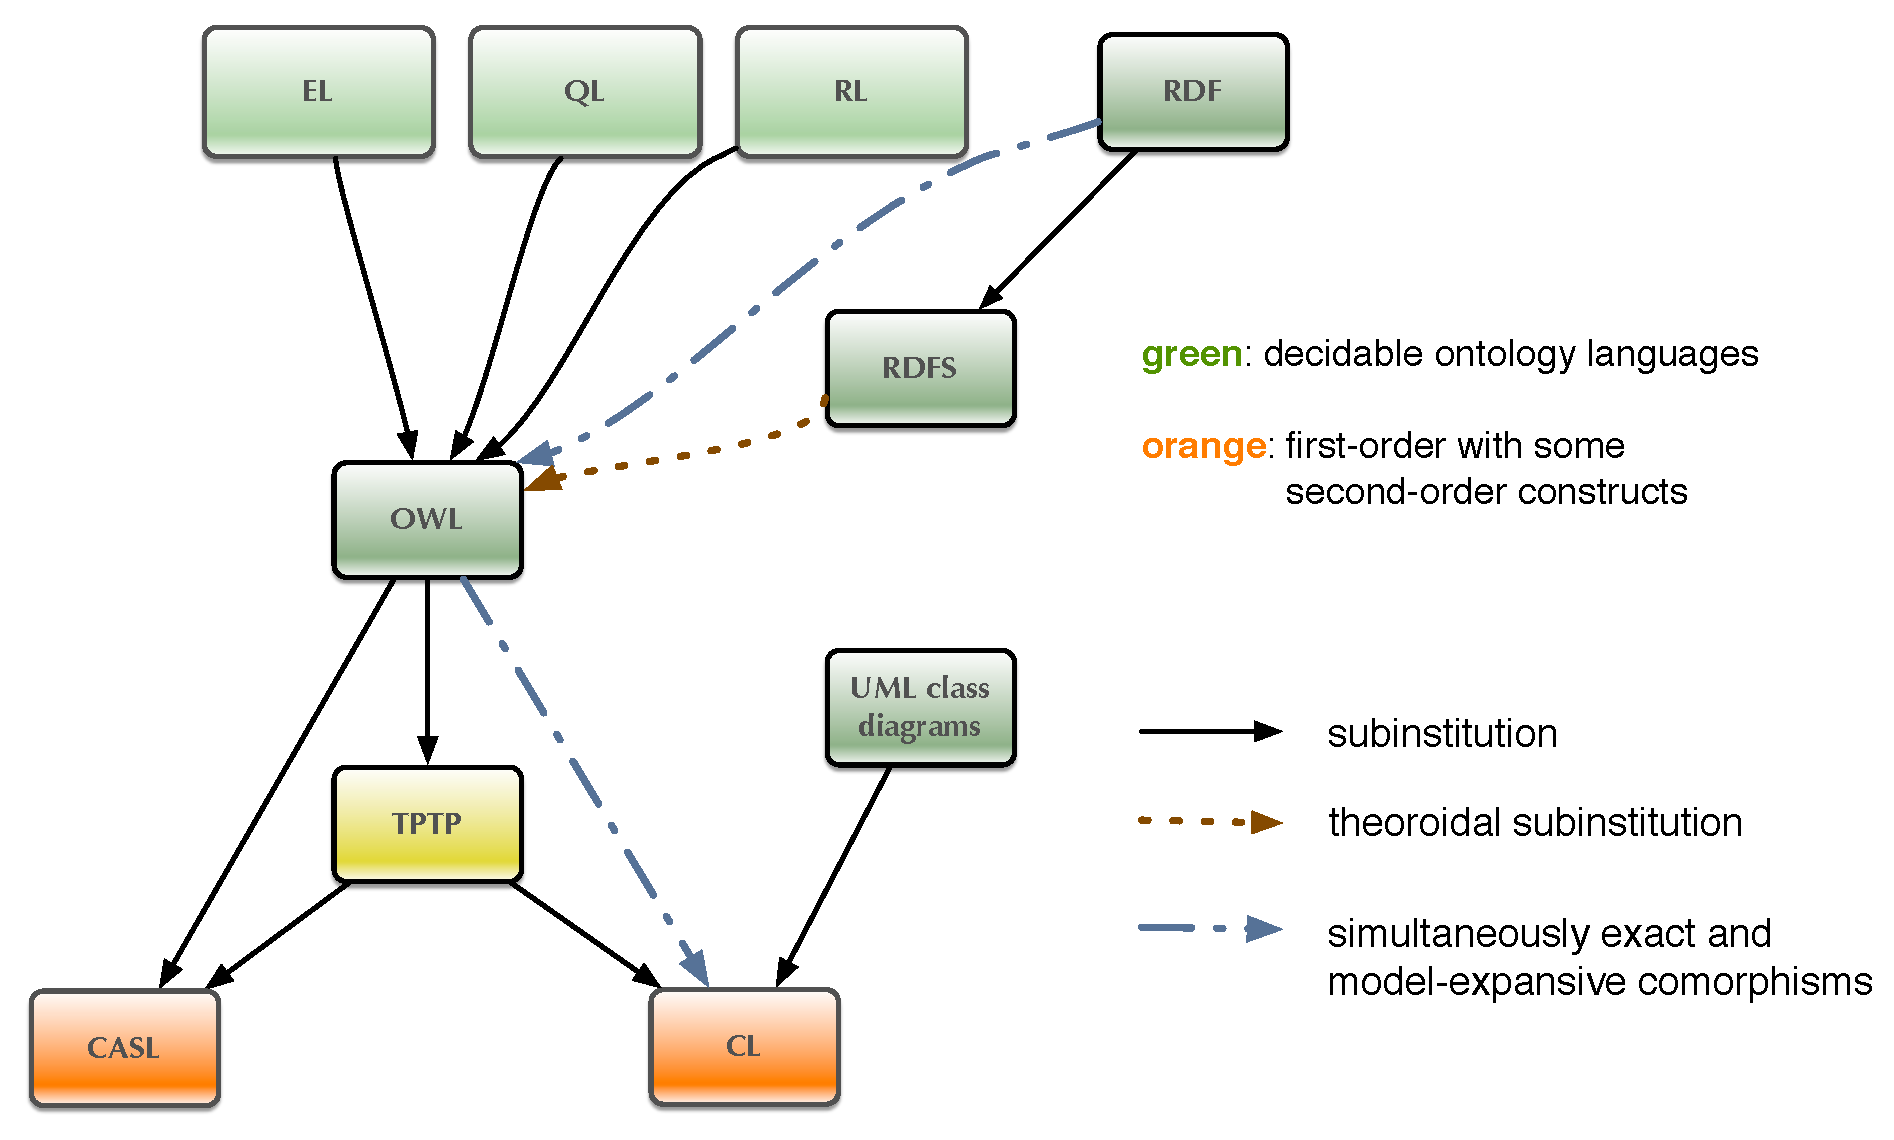
\includegraphics[width=\textwidth]{illustrations/ontograph-standards-new}
  \caption{Translations between conforming OMS languages}
  \label{fig:ontograph-standards}
\end{figure}

This annex provides a core heterogeneous environment that could be used as a basis for 
semantics of \DOL as defined in Sec.~\ref{c:semantics}.

\sclause{Languages}
 
 The OMS languages that we selected
are those whose conformance with \DOL is established in the preceding, normative annexes (OWL 2 DL in \aref{a:owl}, Common Logic in \aref{a:cl}, RDFS in \aref{a:rdfs},
\CASL in \aref{a:casl}, UML class diagrams in \aref{a:uml-class} and TPTP in \aref{a:TPTP}).  The logic graph is shown in \fref{fig:ontograph-standards}; the language graph and supports relation in \fref{f:DOL-threelayers}.  Its nodes refer to the following OMS languages and profiles:
\begin{itemize}
\item RDF \nisref{W3C/TR REC-rdf11-concepts:2014}
\item RDF Schema \nisref{W3C/TR REC-rdf11-schema:2014}
\item EL, QL, RL (all being profiles of OWL) \nisref{W3C/TR REC-owl2-profiles:2009}
\item OWL \nisref{W3C/TR REC-owl2-syntax:2009}
\item CL (Common Logic) \nisref{ISO/IEC 24707:2007}
\item UML class diagrams \nisref{OMG Unified Modeling Language (UML) specification 2.4.1}
\item \CASL \cite{CASL-RM} and its sublanguage classical first-order logic (FOL)
\item TPTP
\end{itemize}

The list of chosen languages includes those ones required as mandatory
ones in the RFP. Since these are only ontology and modeling
languages, also a specification language is included, namely the
Common Algebraic Specification Language (CASL). The list of
language translations, given below, comprises standard translations from the literature,
as well as further translations that are considered useful for
logical interoperability:
\begin{itemize}
  \item \EL $\to$ $\OWL$ 
  \item \QL $\to$ $\OWL$
  \item \RL $\to$ $\OWL$
  \item $\RDF \to \RDFS$
  \item $\RDFS \to \OWL$
  \item $\OWL  \to \CASL.\FOL$
  \item $\CASL.\FOL \to TPTP$
  \item $TPTP \to \CASL.\FOL$
  \item $\CASL.FOL \to \CL$
  \item $\CASL.FOL \to \CASL$
  \item $UML-CD \to \CL$.
\end{itemize}

The translations are specified in \cite{OntoGraph,MossakowskiEtAl14b}.
%~\todonote[author=Christoph Lange,type=todo]{Provide linear syntax here (as in the paper)}
Properties of translations have been introduced in section~\ref{s:foundations}.
All translations are marked as default translations. 

\sclause{Logics}

The logics giving the semantics of these languages are listed below:
\begin{itemize}
 \item \RDF and \RDFS, supported respectively by \RDF and \RDFS
 \item $\ELDL++$, supported by the language \EL
 \item \DLLiteR, supported by \QL
 \item \RL, supported by \RL
 \item $\SROIQ(D)$, supported by $\OWL$
 \item \CL, supported by \CL
 \item $SubPCFOL^=_{ms}$, supported by \CASL
 \item \FOL, supported by $\CASL.FOL$ and $TPTP$
 \item $UML-CD$, supported by $UML-CD$.
\end{itemize}

The institution comorphisms between these logics are
\begin{itemize}
  \item $\ELDL++$ $\to$ $\SROIQ(D)$ 
  \item \DLLiteR $\to$ $\SROIQ(D)$ 
  \item \RL $\to$ $\SROIQ(D)$ 
  \item $\RDF \to \RDFS$
  \item $\RDFS \to \SROIQ(D)$ 
  \item $\SROIQ(D)  \to \CASL.\FOL$
  \item $\FOL \to \CL$
  \item $\FOL \to SubPCFOL^=_{ms}$
  \item $UML-CD \to \CL$.
\end{itemize}

All of them are selected as default logic translations. There are no institution morphisms. The partial union operation between logics is given in the tables below, where
$\bot$ denotes undefinedness:


\begin{tabular}{| l | l | l | l | l | l |}
\hline
Union & $\ELDL++$ & \DLLiteR & \RL & \RDF & \RDFS \\
\hline
$\ELDL++$ & $\ELDL++$ & $\SROIQ(D)$ & $\SROIQ(D)$ & $\SROIQ(D)$ & $\SROIQ(D)$ \\
\hline
\DLLiteR & $\SROIQ(D)$ & \DLLiteR & $\SROIQ(D)$ & $\SROIQ(D)$ & $\SROIQ(D)$ \\
\hline
\RL & $\SROIQ(D)$ &  $\SROIQ(D)$ & \RL & $\SROIQ(D)$ & $\SROIQ(D)$ \\
\hline
\RDF & $\SROIQ(D)$ &  $\SROIQ(D)$ &$\SROIQ(D)$ & \RDF & \RDFS \\
\hline
\RDFS & $\SROIQ(D)$ &  $\SROIQ(D)$ &$\SROIQ(D)$ & \RDFS & \RDFS \\
\hline
$\SROIQ(D)$& $\SROIQ(D)$ &  $\SROIQ(D)$ &$\SROIQ(D)$ & $\SROIQ(D)$ & $\SROIQ(D)$ \\
\hline
\FOL &  \FOL & \FOL & \FOL & \FOL & \FOL \\
\hline
$SubPCFOL^=_{ms}$ &  $SubPCFOL^=_{ms}$ & $SubPCFOL^=_{ms}$ & $SubPCFOL^=_{ms}$ & $SubPCFOL^=_{ms}$ & $SubPCFOL^=_{ms}$ \\
\hline
UML-CD & \CL & \CL & \CL & \CL & \CL \\
\hline
\CL &  \CL & \CL & \CL & \CL & \CL \\
\hline
\end{tabular}

\medskip

\begin{tabular}{| l | l | l | l | l | l |}
\hline
Union & $\SROIQ(D)$ & \FOL & $SubPCFOL^=_{ms}$ & UML-CD & \CL\\
\hline
$\ELDL++$ & $\SROIQ(D)$ & \FOL & $SubPCFOL^=_{ms}$ & \CL & \CL\\
\hline
\DLLiteR & $\SROIQ(D)$ & \FOL & $SubPCFOL^=_{ms}$ & \CL& \CL\\
\hline
\RL  & $\SROIQ(D)$ & \FOL & $SubPCFOL^=_{ms}$ & \CL & \CL\\
\hline
\RDF  & $\SROIQ(D)$ & \FOL & $SubPCFOL^=_{ms}$ & \CL & \CL\\
\hline
\RDFS & $\SROIQ(D)$ & \FOL & $SubPCFOL^=_{ms}$ & \CL & \CL\\
\hline
$\SROIQ(D)$& $\SROIQ(D)$ & \FOL & $SubPCFOL^=_{ms}$ & \CL & \CL\\
\hline
\FOL &  \FOL & \FOL & $SubPCFOL^=_{ms}$ & \CL & \CL\\
\hline
$SubPCFOL^=_{ms}$ & $\SROIQ(D)$ & \FOL & $SubPCFOL^=_{ms}$ & $\bot$ & $\bot$\\
\hline
UML-CD & \CL & \CL & $\bot$ & UML-CD & \CL\\
\hline
\CL & \CL & \CL & $\bot$ & \CL & \CL\\
\hline
\end{tabular}


The other assumptions on the logics in the heterogeneous logical environment hold in
the expected way.\ednote{@Till: rephrase if need be}

\sclause{Serializations}

The following syntaxes are part of the heterogeneous logical environments:
\begin{itemize}
 \item Turtle, supported by $\OWL$, \EL, \QL, \RL , \RDF, \RDFS
 \item RDF-XML, supported by $\OWL$, \EL, \QL, \RL , \RDF, \RDFS
 \item OWL 2 XML, supported by $\OWL$, \EL, \QL, \RL 
 \item Manchester Syntax, supported by $\OWL$, \EL, \QL, \RL
  \item TPTP, supported by TPTP
  \item CASL, supported by \CASL
 \item XMI, supported by UML-CD
 \item XCL, supported by \CL
 \item CLIF, supported by \CL 
\end{itemize}

\sclause{Language and Logic Translations}

\ssclause{\EL $\to$ $\OWL$ and $\ELDL++$ $\to$ $\SROIQ(D)$}

\EL $\to$ $\OWL$ is the sublanguage inclusion obtained by the
syntactic restriction according to the definition of \EL, see
\nisref{W3C/TR REC-owl2-profiles:2009}. Since by definition, $\ELDL++$
is a syntactic restriction of $\SROIQ(D)$, $\ELDL++$ $\to$ $\SROIQ(D)$
is the corresponding sublogic inclusion.

\ssclause{\QL $\to$ $\OWL$ and \DLLiteR $\to$ $\SROIQ(D)$}

\QL $\to$ $\OWL$ is the sublanguage inclusion obtained by the
syntactic restriction according to the definition of \QL, see
\nisref{W3C/TR REC-owl2-profiles:2009}. Since by definition, \DLLiteR
is a syntactic restriction of $\SROIQ(D)$, \DLLiteR $\to$ $\SROIQ(D)$
is the corresponding sublogic inclusion.

\ssclause{\RL $\to$ $\OWL$ and $\RL$ $\to$ $\SROIQ(D)$}

\RL $\to$ $\OWL$ is the sublanguage inclusion obtained by the
syntactic restriction according to the definition of \RL, see
\nisref{W3C/TR REC-owl2-profiles:2009}. Since by definition, $\RL$
is a syntactic restriction of $\SROIQ(D)$, $\RL$ $\to$ $\SROIQ(D)$
is the corresponding sublogic inclusion.

\ssclause{$\SimpleRDF \rightarrow \RDF$}

$\SimpleRDF \rightarrow \RDF$ is an obvious inclusion, except that
\SimpleRDF resources need to be renamed if they happen to have a predefined
meaning in \RDF. The model translation needs to forget the fixed parts
of \RDF models, since this part can always reconstructed in a unique
way, we get an isomorphic model translation. 

\ssclause{$\RDF \rightarrow \RDFS$}

This is entirely analogous to $\SimpleRDF \rightarrow \RDF$.

\ssclause{$\SimpleRDF \rightarrow \SROIQ(D)$}

\todonote{This translation is not really useful. Consider the
  RDF-OWL-reduct construction instead.}


A $\SimpleRDF$ signature is translated to $\SROIQ(D)$ by providing a class
$P$ and three roles $sub$, $pred$ and $obj$ (these reify the extension
relation), and one individual per $\SimpleRDF$ resource. A $\SimpleRDF$ triple
$(s,p,o)$ is translated to the \SROIQ(D) sentence
   $$\top \sqsubseteq \exists U. (\exists sub. \{s\} \sqcap \exists pred. \{p\} \sqcap  \exists obj. \{o\} ).$$
  From an \SROIQ(D) model ${\cal I}$, obtain a \SimpleRDF model by inheriting the universe
  and the interpretation of individuals (then turned into resources).
  The interpretation $P^{\cal I}$ of $P$ gives $P_m$, and $EXT_m$ is obtained
  by de-reifying,
 i.e. $$EXT_{m}(x):=\{(y,z) | \exists u . (u,x)\in pred^{\cal I},
  (u,y)\in sub^{\cal I}, (u,z,)\in obj^{\cal I} \}.$$
  $\RDF \rightarrow \SROIQ(D)$ is defined similarly. The theory of \RDF built-ins 
  is (after translation to \SROIQ(D)) added to any signature translation.
  This ensures that the model translation can add the built-ins.
%\Til{What if the OWL model satisfies more triples than the built-ins?}

\ssclause{$\OWL \rightarrow FOL$}

\sssclause{Translation of signatures}

 $\Phi((\Concepts, \Roles, \Individuals)) =  (F, P)$ with
\begin{itemize}
	\item function symbols: $F = \{a^{(1)} \vert a \in \Individuals\}$
	\item predicate symbols $P = \{A^{(1)} \vert A \in \category{C} \} \cup \{ R^{(2)} \vert R \in \category{R}\}$
\end{itemize}


\sssclause{Translation of sentences}

Concepts are translated as follows:
\begin{itemize}
 \item $\alpha_x(A) = A(x)$
 \item $\alpha_x(\lnot C) = \lnot \alpha_x (C)$
 \item $\alpha_x(C \sqcap D) = \alpha_x(C) \land \alpha_x(D)$
 \item $\alpha_x(C \sqcup D) = \alpha_x(C) \lor \alpha_x(D)$ 
 \item $\alpha_x(\exists R.C) = \exists y . (R(x,y) \land \alpha_y(C))$
 \item $\alpha_x(\exists U.C) = \exists y . \alpha_y(C)$
 \item $\alpha_x(\forall R.C) = \forall y . (R(x,y) \rightarrow \alpha_y(C))$
 \item $\alpha_x(\forall U.C) = \forall y . \alpha_y(C)$
 \item $\alpha_x(\exists R.\text{Self}) = R(x,x)$
 \item $\alpha_x(\leq n R. C) = \forall y_1,\ldots,y_{n+1} .  \bigwedge_{i=1,\ldots,n+1}(R(x,y_i) \land \alpha_{y_i}(C)) \rightarrow\bigvee_{1\leq i<j\leq n+1}y_i = y_j$
 \item $\alpha_x(\geq n R. C) = \exists y_1,\ldots,y_n . \bigwedge_{i=1,\ldots,n}(R(x,y_i) \land \alpha_{y_i}(C)) \wedge \bigwedge_{1\leq i<j\leq n}y_i\not= y_j $
 \item $\alpha_x(\{a_1, \ldots a_n \}) = (x=a_1\vee \ldots \vee x=a_n)$
\end{itemize}

For inverse roles $R^-$, $R^-(x,y)$ has to be replaced by $R(y,x)$, e.g.
 $$\alpha_x(\exists R^-.C) = \exists y . (R(y,x) \land \alpha_y(C))$$
This rule also applies below.


Sentences are translated as follows:

\begin{itemize}
 \item $\alpha_\Sigma (C \sqsubseteq D) = \forall x.\, (\alpha_x(C) \rightarrow \alpha_x(D))$
 \item $\alpha_\Sigma (a:C) = \alpha_x(C)[a/x]$\footnote{$t[a/x]$ means ``in $t$, replace $x$ by $a$''.}
 \item $\alpha_\Sigma (R(a,b)) = R(a,b)$
 \item $\alpha_\Sigma (R \sqsubseteq S) = \forall x, y. R(x,y) \rightarrow S(x,y) $
 \item $\alpha_\Sigma (R_1; \ldots; R_n \sqsubseteq R) =$\\
$ \forall x,y . (\exists z_1,\ldots z_{n-1} . R_1(x,z_1) \wedge R_2(z_1,z_2) \wedge \ldots \wedge R_n(z_{n-1},y)) \rightarrow R(x,y) $
 \item $\alpha_\Sigma (\text{Dis}(R_1,R_2)) = \neg\exists x,y . R_1(x,y)\wedge R_2(x,y)$	
 \item $\alpha_\Sigma (\text{Ref}(R)) = \forall x. R(x,x)$
 \item $\alpha_\Sigma (\text{Irr}(R)) = \forall x. \neg R(x,x)$
 \item $\alpha_\Sigma (\text{Asy}(R)) = \forall x,y . R(x,y) \rightarrow \neg R(y,x)$
 \item $\alpha_\Sigma (\text{Tra}(R)) = \forall x,y,z . R(x,y) \wedge R(y,z) \rightarrow R(x,z)$
\end{itemize}





\sssclause{Translation of models}

\begin{itemize}
	\item For $M' \in \Models^{FOL}(\Phi \Sigma)$ define $\beta_\Sigma(M') := (\Delta, \cdot^I)$
	with $\Delta = |M'|$ and $A^I = M'_A, a^I = M'_a, R^I = M'_R$.
\end{itemize}

	\begin{proposition}
$C^\I = \left\{m \in M'_{\Thing} \lvert M' + \{x \mapsto m \} \models \alpha_x (C) \right\}$
	\end{proposition}
	
	\begin{proof} By Induction over the structure of $C$.
\begin{itemize}
	\item $A^\I = M'_A = \left \{m \in M'_{\Thing} \vert M' + \{x \mapsto m \} \models A(x)  \right\}$
	\item $(\lnot C)^\I = \Delta \setminus C^\I =^{I.H.} \Delta \setminus \{m \in M'_\Thing \lvert M' + \{x \mapsto m\} \models \alpha_x(C)\} = \{m \in M'_\Thing \vert M' + \{x \mapsto m\} \models \lnot \alpha_x(C)\}$
\end{itemize}
	\end{proof}

	The satisfaction condition holds as well.

\ssclause{$FOL \rightarrow \CL$}

This comorphism  maps classical first-order logic (FOL) to Common Logic.

%It maps constants to
%  discourse names and function and predicate symbols to non-discourse
%  names, with a straightforward sentence and model translation;

A FOL signature is translated to \Clogic.Fol by turning all constants
into discourse names, and all other function symbols and all predicate
symbols into non-discourse names. A FOL sentence is translated
to \Clogic.Fol by a straightforward recursion, the base being translations
of predications:
$$\alpha_\Sigma(P(t_1,\ldots,t_n)) = (P\ \alpha_\Sigma(t_1)\ \ldots\ \alpha_\Sigma(t_n))$$
Within terms, function applications are translated similarly:
$$\alpha_\Sigma(f(t_1,\ldots,t_n)) = (f\ \alpha_\Sigma(t_1)\ \ldots\ \alpha_\Sigma(t_n))$$
A \Clogic.Fol model is translated to a FOL model by using the universe of
discourse as FOL universe. The interpretation of constants is
directly given by the interpretation of the corresponding names
in \Clogic.Fol. The interpretation of a predicate symbol $P$ is given
by using $rel^M(int^M(P))$ and restricting to the arity of $P$;
similarly for function symbols (using $fun^M$). Both the satisfaction condition
and model-expansiveness of the comorphism are straightforward.

\ssclause{$\OWL \rightarrow \CL$}

This comorphism is the composition of the comorphisms described in the previous
two sections.

\ssclause{UML class diagrams $\to \CL$}
This translation has been described in annex~\ref{a:uml-class}. 
Translation of signatures is detailed in section~\ref{a:UML-CD-models},
translation of sentences in section~\ref{a:UML-CD-sat}.
Models are translated identically.

\ssclause{$FOL \to \CASL$}
This is an obvious sublogic.
 
\infannex{Extended Logic Graph}\label{a:ext-graph}

\begin{figure}
  \centering
  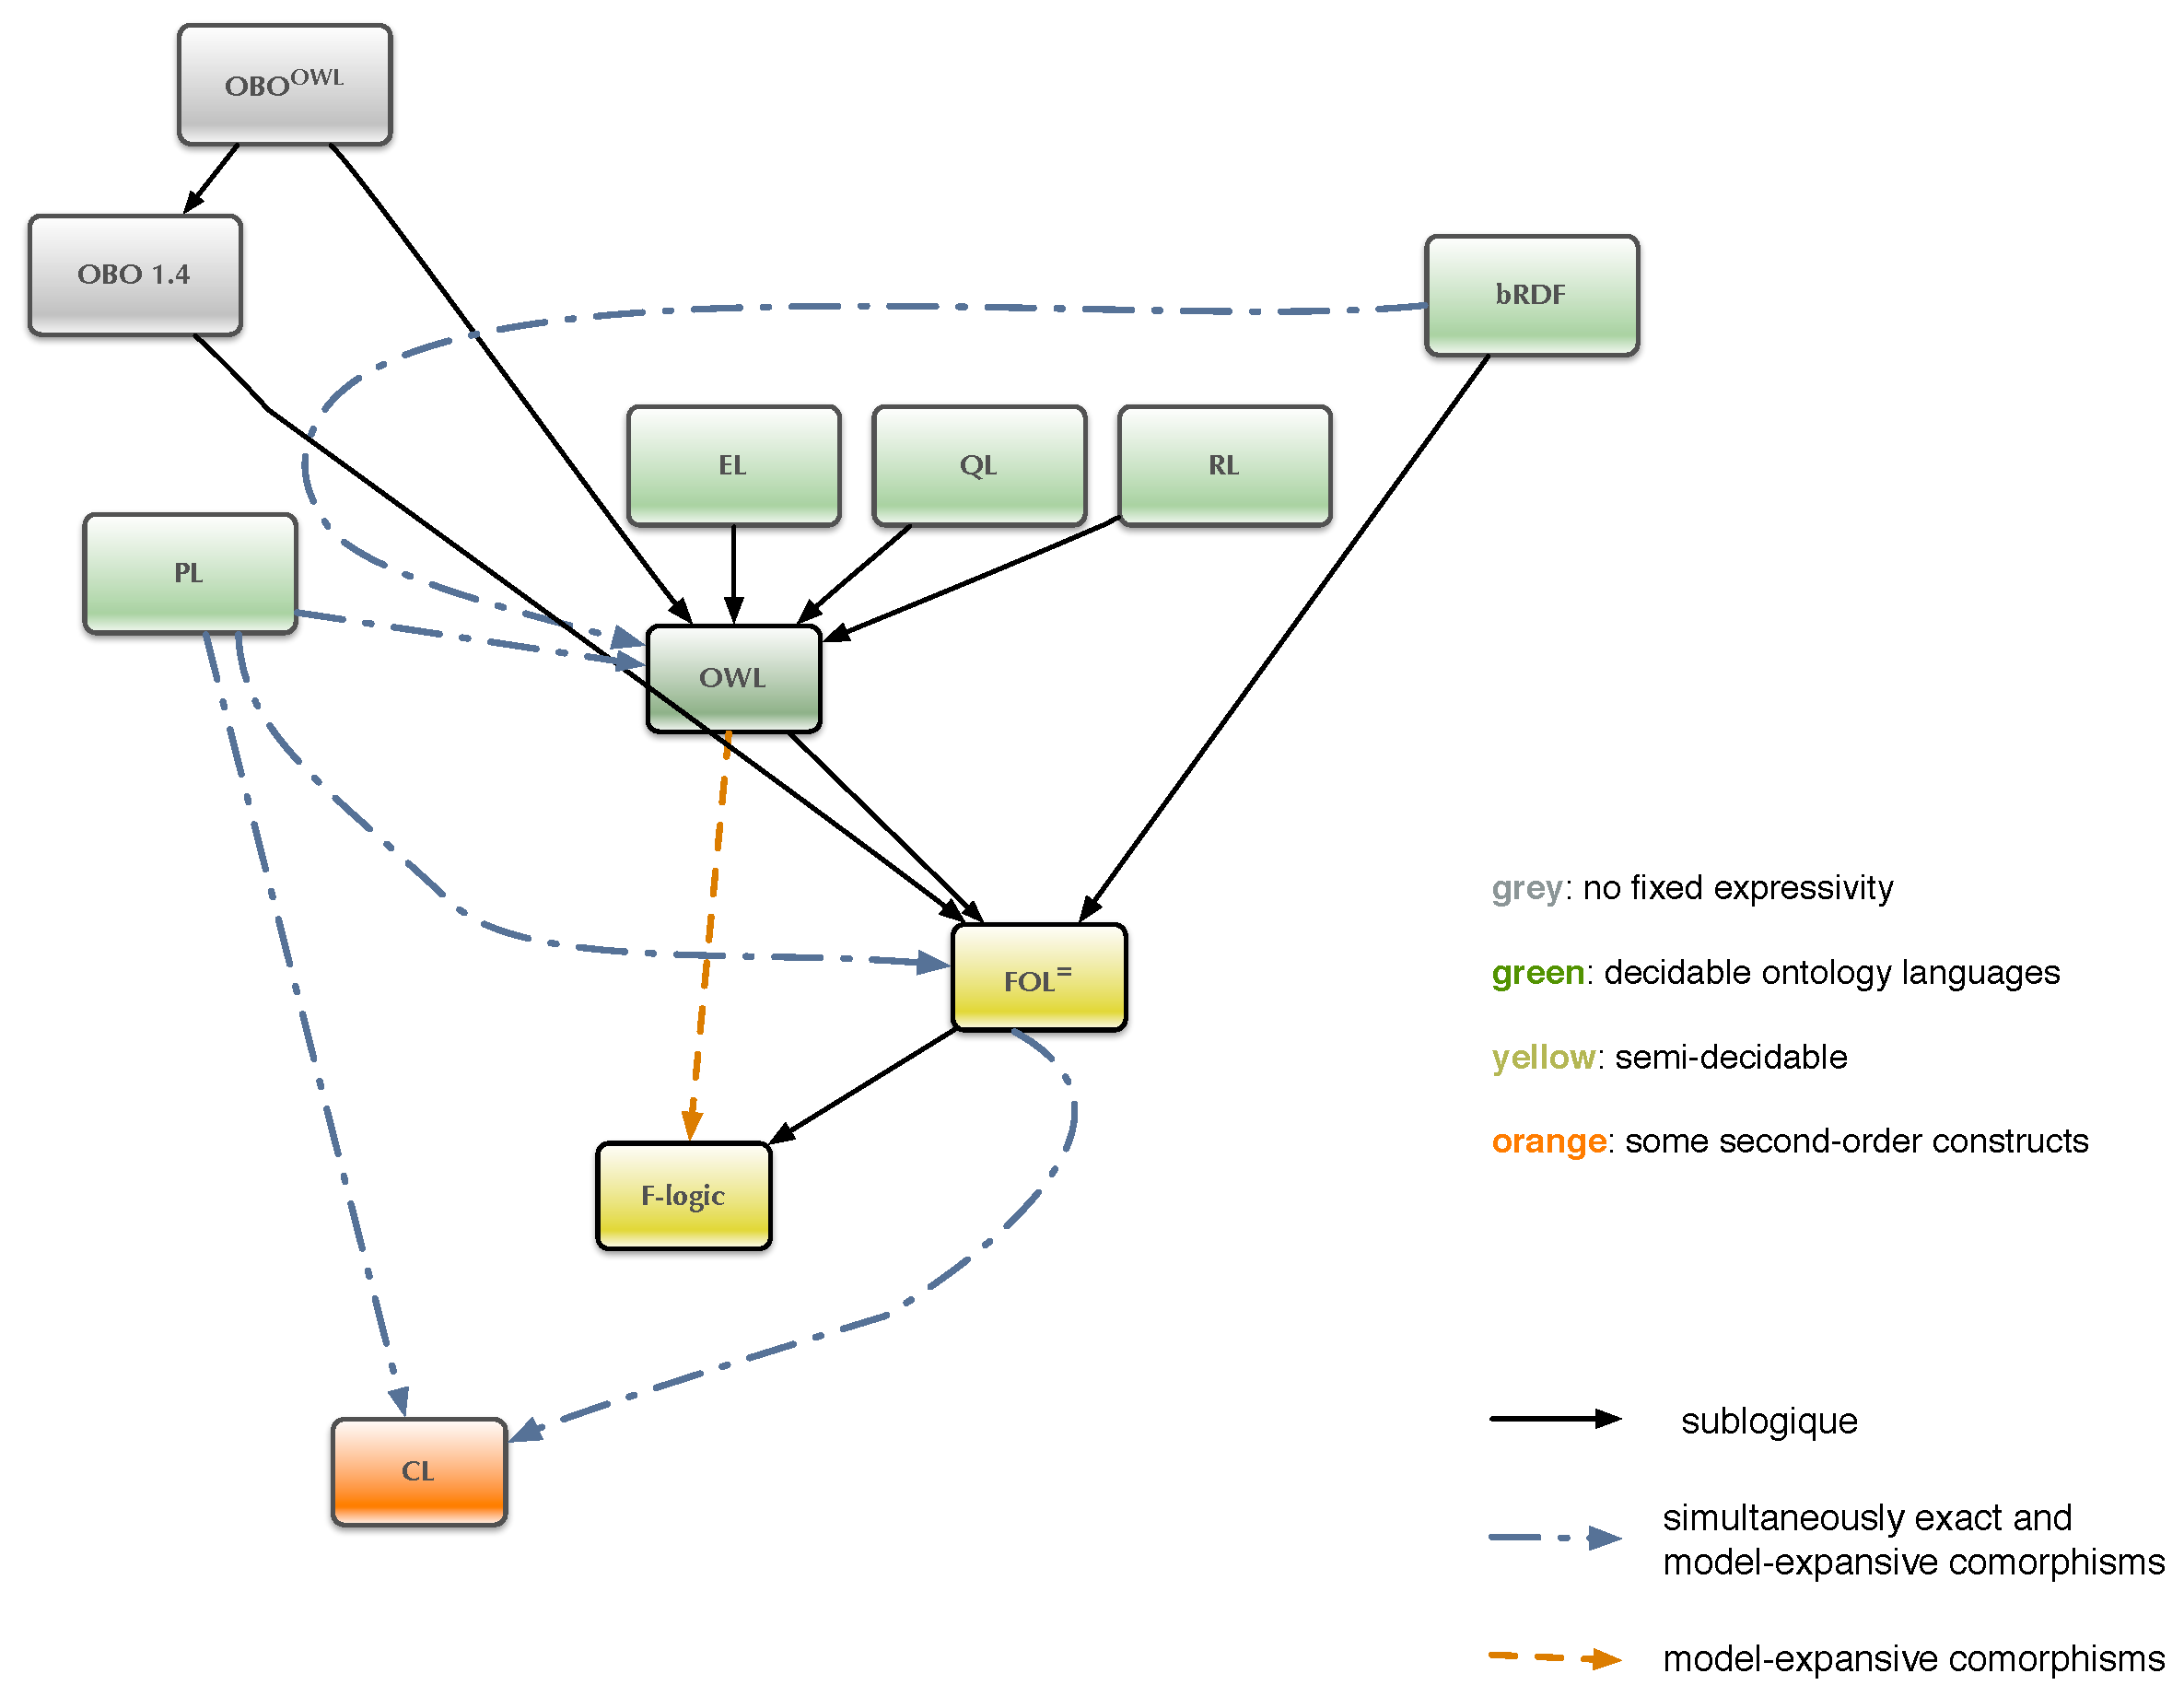
\includegraphics[width=\textwidth]{illustrations/pre-reduced-ontograph}
  \caption{Translations between conforming OMS languages (extended)}
  \label{fig:pre-ontograph}
\end{figure}
This annex extends the graph of logics and translations given in
\aref{a:graph} by a list of OMS language whose conformance with
DOL will be established through the registry.  The graph is shown in
\fref{fig:pre-ontograph}.  Its nodes are included in the following
list of OMS languages and profiles (in addition to those
mentioned in \aref{a:graph}):
\begin{itemize}
\item PL (propositional logic)
\item SimpleRDF (RDF triples without a reserved vocabulary)
\item OBO\textsuperscript{OWL} and OBO1.4
\item RIF (Rule Interchange Format)
\item EER (Enhanced Entity-Relationship Diagrams) % see Talheim Thalheim, B. (2009). Extended entity relationship model. In L. Liu and M. T. Ozsu, editors, En- cyclopedia of Database Systems, volume 1, pages 1083-1091. Springer.
\item Datalog
\item ORM (object role modeling)
\item the meta model of schema.org
\item different diagram types of the UML (Unified Modeling Language), with possibly different logics according to different
UML semantics
\item SKOS (Simple Knowledge Organization System )
\item FOL\textsuperscript{=} (untyped first-order logic, as used for the
TPTP format)
\item F-logic
%\item CASL (Common Algebraic Specification Language)
\end{itemize}

The actual translations are specified in \cite{OntoGraph}.

%~\todonote[author=Christoph Lange,type=todo]{Provide linear syntax here (as in the paper). TM: what do you mean by this?}



\infannex{Example Uses of all \DOL Constructs}\label{a:uses}
\cbs
This annex provides example uses of \DOL constructs.  Jointly with
chapter~\ref{c:goal}, which already contains \DOL examples for the
usage scenarios, all \DOL constructs (although not necessarily all
variants of each construct) are covered.  The examples follow the \DOL
Text Serialization (chapter ~\ref{a:text-syntax}). The following table
provides an overview of which \DOL language constructs have been 
covered where.
\cbe


%\CLnote[type=q-aut]{Should we have another column here that refers to the \emph{abstract} syntax?}%
\begin{tabular}{|l|l|}\hline
\multicolumn{2}{|c|}{\textbf{Top-level declarations in libraries}}\\\hline
\textbf{Top-level declaration} & \textbf{Examples} \\\hline
library \ldots & all examples\\\hline
import IRI & Mereology\\\hline
language IRI  & Alignments, Publications \\\hline
logic IRI  & Alignments, Mereology \\\hline
serialization IRI  & Alignments, Mereology \\\hline
PrefixMap  & Mereology \\\hline
oms IRI = OMS end  &  Alignments, Mereology \\\hline
oms IRI = \%consistent OMS end  & PropositionalExamples, Mereology \\\hline
oms IRI = \%inconsistent OMS end  & PropositionalExamples \\\hline
oms IRI = \%mono OMS end  & section~\ref{spec-2} \\\hline
oms IRI = \%def OMS end  & PropositionalExamples \\\hline
network IRI = IRI, \ldots, IRI & Alignments \\\hline
%network IRI = IRI, \ldots, IRI & \\
%\qquad excluding IRI, \ldots, IRI -> IRI & \\\hline
interpretation IRI : OMS to OMS = SymbolMap  & Mereology \\\hline
interpretation IRI : OMS to OMS = \%cons SymbolMap  &  Engine\\\hline
interpretation IRI : OMS to OMS = translation IRI  & Mereology \\\hline
refinement IRI = OMS refined via SymbolMap to OMS & section~\ref{spec-2} \\\hline
refinement IRI = OMS refined via translation IRI to OMS & section~\ref{model-2} \\\hline
refinement IRI = IRI then IRI & section~\ref{spec-2} \\\hline
refinement IRI = Network refined to Network & section~\ref{model-1} \\\hline
entailment IRI = OMS entails OMS & PropositionalExamples \\\hline
entailment IRI = OMSName in Network entails OMS & section~\ref{model-1}\\\hline
entailment IRI = Network entails Network & section~\ref{model-1}\\\hline
equivalence IRI : OMS \lessthan-\greaterthan\ OMS = OMS end  &  Algebra \\\hline
%equivalence IRI : Network \lessthan-\greaterthan\ Network = Network end  &  \\\hline
module IRI : OMS of OMS for Symbols  & section~\ref{onto-3} \\\hline
%module IRI \%ccons : OMS of OMS for Symbols  &  \\\hline
%alignment IRI : OMS to OMS end  &  \\\hline
%alignment IRI 1 : OMS to OMS end  &  \\\hline
%alignment IRI ? : OMS to OMS end  &  \\\hline
%alignment IRI + : OMS to OMS end  &  \\\hline
%alignment IRI * : OMS to OMS end  &  \\\hline
alignment IRI : OMS to OMS = Correspondences  & Alignments \\\hline
alignment IRI : OMS to OMS = Correspondences & \\
\qquad assuming SingleDomain & \cite{OM2014} \\\hline
alignment IRI : OMS to OMS = Correspondences & \\
\qquad assuming GlobalDomain & \cite{OM2014} \\\hline
alignment IRI : OMS to OMS = Correspondences & \\
\qquad assuming ContextualizedDomain & \cite{OM2014} \\\hline
query IRI = select ars where Sen in OMS & MyQuery\\\hline
substitution IRI : OMS to OMS = SymbolMap & MyQuery\\\hline
result IRI = IRIs for IRI & MyQuery\\\hline
\end{tabular}

\begin{tabular}{|l|l|}\hline
\multicolumn{2}{|c|}{\textbf{OMS}}\\\hline
\textbf{OMS notation} & \textbf{Examples} \\\hline
BasicOMS  & Alignments, Mereology \\\hline
IRI  & Alignments, Mereology \\\hline
%IRI \%( IRI )\%  &  \\\hline
minimize \{ OMS \}  & BlocksWithCircumscription \\\hline
OMS minimize Symbols var Symbols  & BlocksWithCircumscription \\\hline
OMS maximize Symbols var Symbols  & BlocksWithCircumscription \\\hline
%OMS then minimize \{ OMS \} &  \\\hline
%OMS then maximize \{ OMS \} &  \\\hline
free \{ OMS \} & Datatypes \\\hline
cofree \{ OMS \} & Datatypes \\\hline
OMS with SymbolMap  & Alignments,  section~\ref{spec-2} \\\hline
OMS with translation IRI  & Mereology \\\hline
%OMS with translation IRI : IRI $\to$ IRI  &  \\\hline
%OMS with translation IRI $\to$ IRI  &  \\\hline
%OMS with translation $\to$ IRI  &  \\\hline
OMS hide SymbolItems  &  Algebra \\\hline
OMS reveal Symbols  & Datatypes \\\hline
%OMS reveal Symbol |-> Symbol ...  &  \\\hline
OMS hide along IRI  & section~\ref{model-1} \\\hline
%OMS hide along IRI : IRI $\to$ IRI  &  \\\hline
%OMS hide along IRI $\to$ IRI  &  \\\hline
%OMS hide along $\to$ IRI  &  \\\hline
OMS extract Symbols  & section~\ref{onto-3} \\\hline
OMS remove Symbols  & All\_kinds\_of\_group\_specifications \\\hline
OMS forget Symbols  & All\_kinds\_of\_group\_specifications \\\hline
%OMS forget Symbols keep Logic  &  \\\hline
OMS keep Symbols  & All\_kinds\_of\_group\_specifications \\\hline
%OMS keep Symbols keep Logic &  \\\hline
OMS select BasicOMS  & All\_kinds\_of\_group\_specifications  \\\hline
OMS reject BasicOMS  & All\_kinds\_of\_group\_specifications \\\hline
OMS and OMS   & Engine \\\hline
OMS then OMS  & Mereology \\\hline
OMS then \%ccons OMS  &  \cite{DBLP:conf/ijcai/LutzWW07} \\\hline
%OMS then \%ccons \%( IRI )\% OMS  &  \\\hline
OMS then \%mcons OMS  & Propositional \\\hline
OMS then \%notccons OMS  & \cite{DBLP:conf/ijcai/LutzWW07} \\\hline
OMS then \%notmcons OMS  & \cite{DBLP:conf/ijcai/LutzWW07} \\\hline
OMS then \%mono OMS  & Sorting \\\hline
%OMS then \%wdef OMS  &  \\\hline
OMS then \%def OMS  & Persons \\\hline
OMS then \%implied OMS  &  BlocksWithCircumscription \\\hline
logic IRI : OMS  &  all examples\\\hline
language IRI : OMS  &  Mereology\\\hline
serialization IRI : OMS  & Mereology \\\hline
combine NetworkElements  & Alignments, Publications \\\hline
%combine NetworkElements excluding IRIs  &  \\\hline
\end{tabular}

\sclause{Simple Examples in Propositional Logic}
\begin{lstlisting}[basicstyle=\ttfamily,language=dolText,morekeywords={props,ObjectProperty,Class,DisjointUnionOf,SubClassOf,Characteristics,Transitive,Asymmetric,SubPropertyOf,DisjointClasses,EquivalentTo,inverse,only,forall,iff,if,or,exists},escapechar=@,mathescape]
%prefix( :      <http://www.example.org/prop#>
         log:   <http://www.omg.org/spec/DOL/logics/> )%     

		 		%% descriptions of logics ...

%% non-standard serialization built into Hets: 
logic log:Propositional syntax ser:Prop/Hets       

library PropositionalExamples

oms Consistent = %consistent
  props A, B
  . A => B
end

oms Inconsistent = %inconsistent
  props A
  . A /\ not A
end

oms SingleModel = %def
  props A, B
  . A /\ not B
end

entailment Ent = SingleModel entails { . not ( A=>B ) }
end


library PropositionalMereology

%% non-standard serialization built into Hets: 
logic log:Propositional syntax ser:Prop/Hets       

%% basic taxonomic information about mereology reused from DOLCE:
ontology Taxonomy = %conssistent      
  props PT, T, S, AR, PD
  . S $\vee$ T $\vee$ AR $\vee$ PD $\longrightarrow$ PT                                                    %% PT is the top concept
  . S $\wedge$  T  $\longrightarrow$ $\bot$                  %% PD, S, T, AR are pairwise disjoint
  . T $\wedge$ AR $\longrightarrow$ $\bot$                                                                         %% and so on
end
\end{lstlisting}

\sclause{Engine Diagnosis and Repair}\label{engine}

\begin{lstlisting}[basicstyle=\ttfamily,language=dolText,morekeywords={props,ObjectProperty,Class,DisjointUnionOf,SubClassOf,Characteristics,Transitive,Asymmetric,SubPropertyOf,DisjointClasses,EquivalentTo,inverse,only,forall,iff,if,or,exists,import},escapechar=@,mathescape]
library Engine

logic Propositional

%% possible symptoms of an engine that is malfunctioning
spec EngineSymptoms =
  props black_exhaust, blue_exhaust, low_power, overheat,
	ping, incorrect_timing,	low_compression
end

%% diagnosis derived from symptoms
spec EngineDiagnosis = EngineSymptoms
then %mcons
  props carbon_deposits,
	clogged_filter,
	clogged_radiator,
	defective_carburetor,
	worn_rings,
	worn_seals
  . overheat /\ not incorrect_timing => clogged_radiator
                          %(diagnosis1)%
  . ping /\ not incorrect_timing => carbon_deposits
                          %(diagnosis2)%
  . low_power /\ not incorrect_timing =>
                worn_rings \/ defective_carburetor \/ clogged_filter
                          %(diagnosis3)%
  . black_exhaust => defective_carburetor \/ clogged_filter
                          %(diagnosis4)%
  . blue_exhaust => worn_rings \/ worn_seals
                          %(diagnosis5)%
  . low_compression <=> worn_rings
                          %(diagnosis6)%
end

%% needed repair, derived from diagnosis
spec EngineRepair = EngineDiagnosis
then %cons
  props replace_auxiliary,
	repair_engine,
	replace_engine
  . worn_rings => replace_engine
                          %(rule_replace_engine)%
  . carbon_deposits \/ defective_carburetor \/ worn_seals =>
                repair_engine
                          %(rule_repair_engine)%
  . clogged_filter \/ clogged_radiator => replace_auxiliary
                          %(rule_replace_auxiliary)%
end

%% application to a specific case
spec MyObservedSymptoms =
  EngineSymptoms
then
  . overheat              %(symptom_overheat)%
  . not incorrect_timing  %(symptom_not_incorrect_timing)%
end

spec MyRepair =
  MyObservedSymptoms
and 
  EngineRepair
end

spec Repair =
  prop repair
  . repair
end

interpretation repair1 : Repair to MyRepair = %cons
  repair |-> replace_engine end
interpretation repair2 : Repair to MyRepair = %cons
  repair |-> repair_engine end
interpretation repair3 : Repair to MyRepair = %cons
  repair |-> replace_auxiliary end 
%% only repair3 is a valid interpretation. That is, 'replace_auxiliary'
%% is the required action
\end{lstlisting}


\sclause{Mereology: Distributed and Heterogeneous Ontologies}
\label{dist-het-onto}
\begin{lstlisting}[basicstyle=\ttfamily,language=dolText,morekeywords={props,ObjectProperty,Class,DisjointUnionOf,SubClassOf,Characteristics,Transitive,Asymmetric,SubPropertyOf,DisjointClasses,EquivalentTo,inverse,only,forall,iff,if,or,exists,import},escapechar=@,mathescape]
%prefix( :      <http://www.example.org/mereology#>
         owl:   <http://www.w3.org/2002/07/owl#>
         log:   <http://www.omg.org/spec/DOL/logics/>    
		 		%% descriptions of logics ...
         trans: <http://www.omg.org/spec/DOL/translations/> )%  
		 		%% ... and translations

library Mereology

import PropositionalMereology

%% OWL Manchester syntax declaration: 
language lang:OWL2 logic log:SROIQ syntax ser:OWL2/Manchester           

%% Parthood in SROIQ, as far as easily expressible:
ontology BasicParthood =                             
  Class: ParticularCategory 
  	SubClassOf: Particular
                %% omitted similar declarations of the other classes
    DisjointUnionOf: SpaceRegion, TimeInterval, AbstractRegion, Perdurant
                %% pairwise disjointness more compact 
				%% thanks to an OWL built-in
  ObjectProperty: isPartOf        
  	Characteristics: Transitive
  ObjectProperty: isProperPartOf  
  	Characteristics: Asymmetric  SubPropertyOf: isPartOf 
  Class: Atom 
  	EquivalentTo: inverse isProperPartOf only owl:Nothing
end             %% an atom has no proper parts

%% translate the logic, then rename the entities
interpretation TaxonomyToParthood : Taxonomy to BasicParthood =
  translation trans:PropositionalToSROIQ,
  PT $\mapsto$ Particular,	S $\mapsto$ SpaceRegion, 
  T $\mapsto$ TimeInterval,	A $\mapsto$ AbstractRegion, %[ and so on ]%

logic log:CommonLogic syntax ser:CommonLogic/CLIF
                %% syntax: the Lisp-like CLIF dialect of Common Logic

%% ClassicalExtensionalParthood imports the OWL ontology from above, 
%% translate it to Common Logic, then extend it there:
ontology ClassicalExtensionalParthood =
  BasicParthood with translation trans:SROIQtoCL
then
  . (forall (X) (if (or (= X S) (= X T) (= X AR) (= X PD))
                    (forall (x y z) (if (and (X x) (X y) (X z))
                                        (and                          
%% now list all the axioms: 
	%% antisymmetry:
      (if (and (isPartOf x y) (isPartOf y x)) (= x y)) 
	%% transitivity; not combinable with asymmetry in OWL DL:
      (if (and (isProperPartOf x y) (isProperPartOf y z)) (isProperPartOf x z))
      (iff (overlaps x y) (exists (pt) (and (isPartOf pt x) (isPartOf pt y))))
      (iff (isAtomicPartOf x y) (and (isPartOf x y) (Atom x)))
      (iff (sum z x y)
           (forall (w) (iff 
		   	  (overlaps w z) 
			  (and (overlaps w x) (overlaps w y)))))
 %% existence of the sum:
      (exists (s) (sum s x y))                                          
      )))))
%% definition of fusion	  
  . (forall (Set a) (iff (fusion Set a)                                  
            (forall (b) (iff (overlaps b a)
                             (exists (c) (and (Set c) (overlaps c a)))))))
  }
\end{lstlisting}

\sclause{Defined Concepts}
\begin{lstlisting}[basicstyle=\ttfamily,language=dolText,morekeywords={props,ObjectProperty,Class,DisjointUnionOf,SubClassOf,Characteristics,Transitive,Asymmetric,SubPropertyOf,DisjointClasses,EquivalentTo,inverse,only,forall,iff,if,or,exists},escapechar=@,mathescape]
library Persons
logic OWL

ontology Persons =
  Class Person
  Class Female
then %def
  Class: Woman  EquivalentTo: Person and Female
end
\end{lstlisting}


\sclause{Blocks World: Minimization}
\CLnote[type=q-aut]{Here we need the prefixes for registry entries (e.g.\ logics) once more; they should be reused across examples.  Or we need to specify a mechanism that gets rid of \emph{these} prefixes altogether.  @TM, could you please comment on my specification enhancement request \texttt{http://trac.informatik.uni-bremen.de:8080/hets/ticket/1020\#comment:33}?}
  \begin{lstlisting}[language=dolText,morekeywords={forall,if,not,Class,Individual,Types,EquivalentTo,SubClassOf,and}]
library BlocksWithCircumscription
logic log:OWL

ontology Blocks = 
  %% FIXED PART 
  Class: Block
  Individual: B1 Types: Block
  Individual: B2 Types: Block DifferentFrom: B1
              %% B1 and B2 are different blocks
then
  %% CIRCUMSCRIBED PART
  minimize {
    Class: Abnormal
    Individual: B1 Types: Abnormal
       %% B1 is abnormal
  }
then
  %% VARYING PART
  Class: Ontable 
  Class: BlockNotAbnormal 
  	EquivalentTo: Block and not Abnormal 
	SubClassOf: Ontable 
        %% Normally, a block is on the table
then %implied
  Individual: B2 Types: Ontable
     %% B2 is on the table
end
\end{lstlisting}

\todonote{Instead of Blocks World, perhaps we could specify an ontology that
  uses inheritance networks with exceptions, and then use
  circumscription to axiomatize that ontology.}
 
\begin{lstlisting}[language=dolText,morekeywords={forall,if,not,circ,var,Class,Individual,EquivalentTo,and,SubClassOf}]
ontology Blocks_Alternative =
  Class: Block
  Class: Abnormal
  Individual: B1 Types: Block, Abnormal
  Individual: B2 Types: Block DifferentFrom: B1
              %% B1 and B2 are different blocks
              %% B1 is abnormal
  Class: Ontable 
  Class: BlockNotAbnormal 
  	EquivalentTo: Block and not Abnormal 
	SubClassOf: Ontable 
        %% Normally, a block is on the table
  minimize Abnormal var Ontable, BlockNotAbnormal
then %implied
  Individual: B2 Types: Ontable
     %% B2 is on the table
end

ontology Blocks_Alternative2 =
  Class: Block
  Class: Normal
  Individual: B1 Types: Block, not Normal
  Individual: B2 Types: Block DifferentFrom: B1
              %% B1 and B2 are different blocks
              %% B1 is abnormal
  Class: Ontable 
  Class: NormalBlock
  	EquivalentTo: Block and Normal 
	SubClassOf: Ontable 
        %% Normally, a block is on the table
  maximize Normal var Ontable, BlockNotAbnormal
then %implied
  Individual: B2 Types: Ontable
     %% B2 is on the table
end
\end{lstlisting}

\ssclause{Alignments}
\index{alignment}
\begin{lstlisting}[basicstyle=\ttfamily,language=dolText,morekeywords={props,ObjectProperty,Class,DisjointUnionOf,SubClassOf,Characteristics,Transitive,Asymmetric,SubPropertyOf,DisjointClasses,EquivalentTo,inverse,only,forall,iff,if,or,exists,distributed},escapechar=@,mathescape]
%prefix( :     <http://www.example.org/alignment#>
         owl:   <http://www.w3.org/2002/07/owl#>
         log:   <http://www.omg.org/spec/DOL/logics/> %% descriptions of logics ...
         trans: <http://www.omg.org/spec/DOL/translations/> )% %% ... and translations

library Alignments

language lang:OWL2 logic log:SROIQ syntax ser:OWL2/Manchester

alignment Alignment1 : { Class: Woman } to { Class: Person } =
  Woman < Person
end

ontology AlignedOntology1 =
  combine Alignment1
end


ontology Onto1 =
  Class: Person
  Class: Woman SubClassOf: Person
  Class: Bank
end

ontology Onto2 =
  Class: HumanBeing
  Class: Woman SubClassOf: HumanBeing
  Class: Bank
end

alignment VAlignment : Onto1 to Onto2 =
  Person = HumanBeing,
  Woman = Woman
end

network N =
  1 : Onto1, 2 : Onto2, VAlignment
end
 
ontology VAlignedOntology =
  combine N
  %% 1:Person is identified with 2:HumanBeing
  %% 1:Woman is identified with 2:Woman
  %% 1:Bank and 2:Bank are kept distinct
end

ontology VAlignedOntologyRenamed =
  VAlignedOntology with 1:Bank |-> RiverBank, 2:Bank |-> FinancialBank
end

\end{lstlisting}


\sclause{Distributed Description Logics}

\begin{lstlisting}[basicstyle=\ttfamily,language=dolText,morekeywords={props,ObjectProperty,Class,DisjointUnionOf,SubClassOf,Characteristics,Transitive,Asymmetric,SubPropertyOf,DisjointClasses,EquivalentTo,inverse,only,forall,iff,if,or,exists,distributed},escapechar=@,mathescape]
%prefix( :     <http://www.example.org/mereology#>
         owl:   <http://www.w3.org/2002/07/owl#>
         log:   <http://www.omg.org/spec/DOL/logics/> %% descriptions of logics ...
         trans: <http://www.omg.org/spec/DOL/translations/> )% %% ... and translations

library Publications

language lang:OWL2 logic log:SROIQ syntax ser:OWL2/Manchester

ontology Publications1 =
  Class: Publication
  Class: Article SubClassOf: Publication
  Class: InBook SubClassOf: Publication
  Class: Thesis  SubClassOf: Publication
  Class: MasterThesis  SubClassOf: Thesis
  Class: PhDThesis SubClassOf: Thesis
end

ontology Publications2 =
  Class: Thing
  Class: Article SubClassOf: Thing
  Class: BookArticle SubClassOf: Thing
  Class: Publication SubClassOf: Thing
  Class: Thesis  SubClassOf: Thing
end

ontology Publications_Combined =
combine
  1 : Publications1 with translation OWL2MS-OWL,
  2 : Publications2 with translation OWL2MS-OWL
  %% implicitly: Article $\mapsto$ 1:Article @\ldots@
  %%             Article $\mapsto$ 2:Article @\ldots@  
  with translation MS-OWL2DDL
  %% implicitly added by translation MS-OWL2DDL: 
  %% binary relation providing the bridge
then
  1:Publication $\stackrel{\sqsubseteq}{\longrightarrow}$ 2:Publication
  1:PhdThesis $\stackrel{\sqsubseteq}{\longrightarrow}$ 2:Thesis
  1:InBook $\stackrel{\sqsubseteq}{\longrightarrow}$ 2:BookArticle
  1:Article $\stackrel{\sqsubseteq}{\longrightarrow}$ 2:Article
  1:Article $\stackrel{\sqsupseteq}{\longrightarrow}$ 2:Article
end


ontology Publications_Extended =
Publications with translation DDL2-ECO
  %% turns implicit domain-relation into default relation 'D'
  %% add E-connection style bridge rules on top
end


library Market


language lang:OWL2 logic log:SROIQ syntax ser:OWL2/Manchester
ontology Purchases =
combine
  1 : { Class: PurchaseOrder },
  2 : { ObjectProperty: Buyer
       ObjectProperty: Good
       ObjectProperty: BoughtBy }
  with translation OWL2DDLwithRoles
then
  1:PurchaseOrder -into-> 2:BoughtBy
%% means in FOL: 
%% forall x 1PurchaseOrder(x) -> forall yz CR12(x,y,z) -> 2BoughtBy(y,z)
end


\end{lstlisting}


\sclause{Algebra}


\begin{lstlisting}[basicstyle=\ttfamily,language=dolText,morekeywords={props,ObjectProperty,Class,DisjointUnionOf,SubClassOf,Characteristics,Transitive,Asymmetric,SubPropertyOf,DisjointClasses,EquivalentTo,inverse,only,forall,iff,if,or,exists,distributed,equivalence},escapechar=@,mathescape]
%prefix( :     <http://www.example.org/alignment#>
         owl:   <http://www.w3.org/2002/07/owl#>
         log:   <http://www.omg.org/spec/DOL/logics/> %% descriptions of logics ...
         trans: <http://www.omg.org/spec/DOL/translations/> )% %% ... and translations

library Algebra

logic log:CommonLogic syntax ser:CommonLogic/CLIF

spec implicit_group =
(forall (x y z)
        (= (op x (op y z)) (op (op x y) z)))
(exists (e)
        (forall (x)
                (and    (= x (op e x))
                        (= x (op x e)))))
(forall (x)
        (exists (y)
                (and    (= x (op x (op x y)))
                        (= x (op x (op y x))))))
end

spec explicit_group =
(forall (x y z)
        (= (op x (op y z)) (op (op x y) z)))
(forall (x)     (and    (= x (op e x))
                        (= x (op x e)))))
(forall (x)
                (and    (= x (op x (op x (inv x))))
                        (= x (op x (op (inv x) x))))))
end

equivalence groups_equiv : implicit_group <-> { explicit_group hide e, inv }
end
\end{lstlisting}

\begin{lstlisting}[basicstyle=\ttfamily,language=dolText,morekeywords={props,ObjectProperty,Class,DisjointUnionOf,SubClassOf,Characteristics,Transitive,Asymmetric,SubPropertyOf,DisjointClasses,EquivalentTo,inverse,only,forall,iff,if,or,exists,sort,ops,in,approximate,extract,equivalence,spec},escapechar=@,mathescape]
equivalence e : algebra:BooleanAlgebra
                $\leftrightarrow$ algebra:BooleanRing =
    x$\wedge$y = x$\cdot$y
    x$\vee$y = x+y+x$\cdot$y
    $\neg$x = 1+x
    x$\cdot$y = x$\wedge$y
    x+y = (x$\vee$y) $\wedge$ $\neg$(x$\wedge$y)
end
\end{lstlisting}

\begin{lstlisting}[basicstyle=\ttfamily,language=dolText,morekeywords={props,ObjectProperty,Class,DisjointUnionOf,SubClassOf,Characteristics,Transitive,Asymmetric,SubPropertyOf,DisjointClasses,EquivalentTo,inverse,only,forall,iff,if,or,exists,sort,ops,forget,entails,entailment,spec},escapechar=@,mathescape]
logic CASL

spec InterpolatedGroup =
  sort Elem
  ops 0:Elem; __+__:Elem*Elem->Elem; inv:Elem->Elem
  forall x,y,z:elem . x+0=x
                    . x+(y+z) = (x+y)+z
                    . x+inv(x) = 0
  forget inv
end

entailment ent = InterpolatedGroup 
  entails { . forall x:Elem . exists y . Elem . x+y=0 }
end
\end{lstlisting}

\ssclause{Groups specified with different forms of hiding and forgetting}

\sssclause{Groups and hiding}
\begin{lstlisting}[basicstyle=\ttfamily,language=dolText,morekeywords={props,ObjectProperty,Class,DisjointUnionOf,SubClassOf,Characteristics,Transitive,Asymmetric,SubPropertyOf,DisjointClasses,EquivalentTo,inverse,only,forall,iff,if,or,exists,sort,ops,spec},escapechar=@,mathescape]
library All_kinds_of_group_specifications
logic CASL
spec Group_with_inverse =
  sort Elem
  ops 0:Elem; __+__:Elem*Elem->Elem; inv:Elem->Elem
  forall x,y,z:elem . x+0=x
                    . x+(y+z) = (x+y)+z
                    . x+inv(x)=0
end

spec Group_via_hiding =
  Group_with_inverse hide inv
end
\end{lstlisting}

The semantics of this specification is the class of all monoids that
can be extended with an inverse, i.e.\ class of all groups. The effect
is second-order quantification:

\begin{lstlisting}[basicstyle=\ttfamily,language=dolText,morekeywords={props,ObjectProperty,Class,DisjointUnionOf,SubClassOf,Characteristics,Transitive,Asymmetric,SubPropertyOf,DisjointClasses,EquivalentTo,inverse,only,forall,iff,if,or,exists,sort,ops,spec},escapechar=@,mathescape]
logic HasCASL
spec Group_in_second_order_logic =
  sort Elem
  ops 0:Elem; __+__:Elem*Elem->Elem; 
  exists inv:Elem->Elem .
    forall x,y,z:elem . x+0=x
                        /\ x+(y+z) = (x+y)+z
                        /\ x+inv(x)=0
end
\end{lstlisting}

\sssclause{Groups and module extraction}

\begin{lstlisting}[basicstyle=\ttfamily,language=dolText,morekeywords={props,ObjectProperty,Class,DisjointUnionOf,SubClassOf,Characteristics,Transitive,Asymmetric,SubPropertyOf,DisjointClasses,EquivalentTo,inverse,only,forall,iff,if,or,exists,sort,ops,spec,forget},escapechar=@,mathescape]
logic CASL
spec Group_via_module_extraction_1 =
  Group_with_inverse remove inv
end
\end{lstlisting}
The semantics is just \syntax{Group\_with\_inverse},
since the module needs to be enlarged to the whole specification.
This is of course unsatisfactory. A better use of module extraction
is the following:

\begin{lstlisting}[basicstyle=\ttfamily,language=dolText,morekeywords={props,ObjectProperty,Class,DisjointUnionOf,SubClassOf,Characteristics,Transitive,Asymmetric,SubPropertyOf,DisjointClasses,EquivalentTo,inverse,only,forall,iff,if,or,exists,sort,ops,spec,forget},escapechar=@,mathescape]
logic CASL
spec Group_with_implicit_inverse =
  sort Elem
  ops 0:Elem; __+__:Elem*Elem->Elem; inv:Elem->Elem
  forall x,y,z:elem . x+0=x
                    . x+(y+z) = (x+y)+z
                    . x+inv(x) = 0
                    . exists y:Elem . x+y=0
end

spec Group_via_module_extraction_2 =
  Group_with_implicit_inverse remove inv
end
\end{lstlisting}
The semantics of \syntax{Group\_via\_module\_extraction\_2} is just
\syntax{Group\_with\_implicit\_inverse}, because adding \texttt{inv}
is conservative.
\medskip

\sssclause{Groups via interpolation}

\begin{lstlisting}[basicstyle=\ttfamily,language=dolText,morekeywords={props,ObjectProperty,Class,DisjointUnionOf,SubClassOf,Characteristics,Transitive,Asymmetric,SubPropertyOf,DisjointClasses,EquivalentTo,inverse,only,forall,iff,if,or,exists,sort,ops,spec,forget},escapechar=@,mathescape]
logic CASL
spec Group_via_interpolation1 =
  Group_with_inverse forget inv
end
spec Group_via_interpolation2 =
  Group_with_inverse keep Elem, 0, __+__
end
\end{lstlisting}
Both specifications are equivalent, and they 
are equivalent to \syntax{Group\_with\_implicit\_inverse}.
%Computing interpolants can be hard, even undecidable.
\medskip

\sssclause{Groups and filtering}
\begin{lstlisting}[basicstyle=\ttfamily,language=dolText,morekeywords={props,ObjectProperty,Class,DisjointUnionOf,SubClassOf,Characteristics,Transitive,Asymmetric,SubPropertyOf,DisjointClasses,EquivalentTo,inverse,only,forall,iff,if,or,exists,sort,ops,spec,forget},escapechar=@,mathescape]
logic CASL
spec Group_via_Filtering_1 =
  Group_with_inverse reject inv
end
spec Group_via_Filtering_2 =
  Group_with_inverse select Elem, 0, __+__
end
\end{lstlisting}
Both specifications are equivalent, and they are equivalent 
to the following theory which just omits the inverse
axioms (and hence does not specify groups):
\begin{lstlisting}[basicstyle=\ttfamily,language=dolText,morekeywords={props,ObjectProperty,Class,DisjointUnionOf,SubClassOf,Characteristics,Transitive,Asymmetric,SubPropertyOf,DisjointClasses,EquivalentTo,inverse,only,forall,iff,if,or,exists,sort,ops,spec,forget},escapechar=@,mathescape]
logic CASL
spec Group_via_reject =
  sort Elem
  ops 0:Elem; __+__:Elem*Elem->Elem
  forall x,y,z:elem . x+0=x
                    . x+(y+z) = (x+y)+z
end
\end{lstlisting}





\sclause{Queries}
\begin{lstlisting}[basicstyle=\ttfamily,language=dolText,morekeywords={props,ObjectProperty,Class,DisjointUnionOf,SubClassOf,Characteristics,Transitive,Asymmetric,SubPropertyOf,DisjointClasses,EquivalentTo,inverse,only,forall,iff,if,or,exists,query,select,where,in,substitution,result,for,along,library,spec,sort,pred,op},escapechar=@,mathescape]
library MyQuery
logic CASL
spec Person =
  sort s
  pred Person:s 
  op max,peter:Person
end
query MyQuery = select x where Person(x) in Person
end
substitution MySubst : { Person then op x:Person } to Person = x |-> max
end
result MyResult = MySubst for MyQuery
\end{lstlisting}

\sclause{Datatypes}

\begin{lstlisting}[basicstyle=\ttfamily,language=dolText,morekeywords={props,ObjectProperty,Class,DisjointUnionOf,SubClassOf,Characteristics,Transitive,Asymmetric,SubPropertyOf,DisjointClasses,EquivalentTo,inverse,only,forall,iff,if,or,exists,sort,ops,in,approximate,extract,free,cofree,spec},escapechar=@,mathescape]
library Datatypes
logic CASL

spec Bag =
  sort Elem
  then free {
     sort Bag
     ops mt:Bag;
         __union__:Bag*Bag->Bag, assoc, comm, unit mt
           }
end

spec Stream =
  sort Elem
  then cofree {
     sort Stream
     ops head:Stream->Elem;
         tail:Stream->Stream
           }
end

spec Finite =
  sort Elem
  free type Nat ::= 0 | suc(Nat)
  op f: Nat ->? Elem
  . forall x:Elem . exists n:Nat . f(n)=x           %(f_surjective)%
  . exists n:Nat . forall m:Nat . def f(m) => m<n   %(f_bounded)%
  reveal Elem
end

\end{lstlisting}

\infannex{Use cases}\label{a:use-cases}

This annex sketches scenarios that outline how \DOL is intended to be applied.  For each scenario, we list its status of implementation, the \DOL features it makes use of, and provide a brief description.

\newenvironment{usecase}[3]{\sclause{#1}%
\begin{description}
\item[Status] #2
\item[Features] #3
\end{description}
}{}
\begin{usecase}{Generating multilingual labels for menus in a user interface}{exists (but not yet \DOL-based)}{Aligning (multiple OWL ontologies), Annotation}
  DO-ROAM (\textbf{D}ata and \textbf{O}ntology driven \textbf{R}oute-finding \textbf{O}f \textbf{A}ctivity-oriented \textbf{M}obility\footnote{\url{http://www.do-roam.org}}) is a web service with an interactive frontend that extends OpenStreetMap by an ontology-based search for located activities and opening hours \cite{do-roam}.  The service is driven by a set of different OWL ontologies that have been aligned to each other using the Falcon matching tool \cite{HuQu-08}.  The user interface of the DO-ROAM web frontend offers multilingual labels, which are maintained in close connection to the underlying ontologies.

  Porting DO-ROAM to \DOL would enable the coherent representation of the aligned ontologies as one OMS network, and it would enable  the maintenance of the user interface labels as annotations inside the ontology.
\end{usecase}

\begin{usecase}{Connecting devices of differing complexity in an Ambient Assisted Living setting}{core ontology (not \DOL-based) and service environment exists – the \DOL-based extensions not yet}{Logical OMS mappings across different logics, connection to linked open datasets}
  Consider the following ambient assisted living (AAL) scenario:
  \begin{quote}
    Clara instructs her \textbf{wheelchair} to get her to the \textbf{kitchen} (\textbf{\underline{next door}} to the \textbf{living room}.  For \textbf{dinner}, she would like to take a \textit{pizza} from the \textbf{freezer} and bake it in the \textbf{oven}.  (Her diet is \textit{vegetarian}.)  \textbf{\underline{Afterwards}} she needs to rest in \textbf{bed}.
  \end{quote}
  Existing ontologies for ambient assisted living (\eg the OpenAAL\footnote{\url{http://openaal.org}} OWL ontology) cover the \emph{core} of these  concepts; they provide at least classes (or generic superclasses) corresponding to the concepts highlighted in \textbf{bold}.  However, that does not cover the scenario completely:
  \begin{itemize}
  \item Some concepts (here: food and its properties, \textit{italicized}) are not covered.  There are separate ontologies for that (such as the Pizza ontology\footnote{This is not a fully comprehensive food ontology, but rather a well-known sample OWL ontology; \cf \url{http://owl.cs.manchester.ac.uk/tutorials/protegeowltutorial/}}), whereas information about concrete products (here: information about the concrete pizza in Clara's oven) would rather come from Linked Open Datasets than from formal ontologies.
  \item Not all concepts (here: space and time, \underline{underlined}) are covered at the required level of complexity.  OpenAAL says that appointments have a date and that rooms can be connected to each other, but not what exactly that means.  Foundational ontologies and spatial calculi, often formalized in first-order logic, cover space and time at the level of complexity required by a central controller of an apartment and by an autonomously navigating wheelchair.
  \item Thirdly, even description logic might be too complex for very simple devices involved into the scenario, such as the kitchen light switch, for which propositional logic may be sufficient.
  \end{itemize}
  Thus, an adequate formalization of this scenario has to be heterogeneous.  For example, one could imagine the following axioms:
  \begin{description}
  \item[light switch] ``light is switched on if and only if someone is in the room and it is dark outside'' – this could be formalized in propositional logic as $\mathrm{light\_on}\equiv\mathrm{person\_in\_room}\wedge\mathrm{dark\_outside}$.
  \item[freezer] ``a vegetarian pizza is a pizza whose toppings are all vegetarian'' – this could be formalized in description logic as $\mathrm{VegetarianPizza}\equiv\mathrm{Pizza}\sqcap \forall \mathrm{hasTopping}.\mathrm{Vegetarian}$
  \item[wheelchair] ``two areas in a house (\eg a working area in a room) are either the same, or intersecting, or bordering, or separated, or one is part of the other'' – this could be formalized as an RCC-style spatial calculus in first-order logic as $$\begin{array}{ll}\forall a_1, a_2 . & \mathrm{equal}(a_1, a_2) \veebar \mathrm{overlapping}(a_1, a_2) \veebar \mathrm{bordering}(a_1, a_2) \veebar \mathrm{disconnected}(a_1, a_2) \\
&\veebar \mathrm{part\_of}(a_1, a_2) \veebar \mathrm{part\_of}(a_2, a_1).\end{array}$$
  \end{description}
  
  \DOL would be capable of expressing all that within one library of heterogeneous ontologies arranged around an OWL core (here: the OpenAAL ontology), including OMS mappings from OpenAAL to the other ontologies, as well as a re-declaration of a concrete pizza product from a product dataset as an instance of the Pizza OWL class.
\end{usecase}

\begin{usecase}{Interpreting the OWL formalization of the DOLCE foundational ontology in First-order logic}{potential use case}{Logical OMS mappings}
  DOLCE is a foundational ontology that has primarily been formalized in the first-order logic ontology language KIF (a predecessor of Common Logic), but also in OWL (``DOLCE Lite'') \cite{dolce}. This ‘OWLized’ version was targeting use in semantic web services and domain ontology interoperability, and to provide the generic categories and relationships to aid domain ontology development. DOLCE has been used also for semantic middleware, and in OWL-formalized ontologies of neuroimaging, computing, ecology, and data mining and optimization.
  Given the differences in expressivity, DOLCE Lite had to simplify certain notions.  For example, the DOLCE Lite formalization of ``temporary parthood'' (something is part of something else at a certain point or interval in time) omits any information about the time, as OWL only supports binary predicates (a.k.a.\ ``properties'').  That leaves ambiguities for modeling a view from DOLCE Lite to the first-order DOLCE, as such a view would have to reintroduce the third (temporal) component of such predicates:
  \begin{itemize}
  \item Should a relation asserted in terms of DOLCE Lite be assumed to hold for \emph{all} possible points/intervals in time, \ie should it be universally quantified?
  \item Or should such a relation be assumed to hold for \emph{some} points/intervals in time, \ie should it be existentially quantified?
  \item Or should a concrete value for the temporal component be assumed, \eg ``0'' or ``now''?
  \end{itemize}
  
  \DOL would support the formalization of  all of these views and, given suitable consistency checking tools, the analysis of  whether any such view would satisfy all further axioms that the first-order DOLCE states about temporal parthood.
\end{usecase}

\begin{usecase}{Extending the OWL Time ontology to a more comprehensive coverage of time}{potential use case}{Logical OMS mappings}
The OWL Time ontology\footnote{\url{http://www.w3.org/TR/2006/WD-owl-time-20060927/}} covers temporal concepts such as instants and intervals and has been designed for describing the temporal content of Web pages and the temporal properties of Web services.  While OWL is suitable for these intended applications, only a first-order axiomatization is capable of faithfully capturing all relevant notions, such as the trichotomy of the ``before'' relation: One instant is either before another one, or at the same time, or after.  Moreover, a relationship between facts expressed in terms of instants and facts expressed in terms of intervals (both of which is, independently, possible in OWL), can only be established via first-order logic, \eg by declaring an interval of length zero equivalent to an instant. 

A separate first-order axiomatization of OWL Time exists
[\cite{OWLTime},\cite{OWLSTime}].  \DOL would instead provide the mechanism of modeling
OWL Time as one coherent heterogeneous ontology, using OWL and, \eg,
Common Logic.\footnote{This is also a use case for multiple namespaces:
  OWL supports namespaces, CL does not.}  For the temporal description
logic $\mathcal{DLR_{US}}$ for knowledge bases and logic-based
temporal conceptual data modeling [\cite{Artale02},\cite{Artale07a}];
$\mathcal{DLR_{US}}$ combines the propositional temporal logic with
the {\em Since} and {\em Until} operators and the (non-temporal)
description logic $\mathcal{DLR}$ and can be regarded as an expressive
fragment of the first-order temporal logic $L^{since, until}$. Within
DOL, this would enable one to have `lightweight' time aspects with OWL
Time, which are then properly formalized with $\mathcal{DLR_{US}}$ or
a leaner variant TDL-Lite [\cite{Artale07time}], where notions such as
(some time) ``before'' are given a formal semantics of the intended
meaning that the plain OWL Times human-readable object property does
not have. The latter, then, would enable the modeler to represent the
meaning---hence, restrict the possible models---and check the
consistency of the temporal constraints and so-called `evolution
constraints' in the ontology (evolution constraints constrain
membership of an object or an individual relation to a concept or
relationship over time). For instance, that each divorcee must have
been a participant in a marriage before, that boarding only may occur
after checking in, and that any employee must obtain a salary increase
after two years of employment. It also can be used to differentiate
between essential and immutable parthood, therewith being precise in
the ontology about, e.g., the distinction how a human brain is part of
a human (humans cannot live without it), versus how a hand is part of
a human (humans can live without it), versus how the hand is part of,
say, a boxer, which is essential to the boxer but only for has long as
he is a boxer [\cite{AGK08}].

\end{usecase}

\begin{usecase}{Metadata in COLORE (Common Logic Repository)}{exists (but not yet \DOL-based)}{Annotation, Metadata vocabularies}
  COLORE, the Common Logic Repository\footnote{\url{http://stl.mie.utoronto.ca/colore/}} is an open repository of more than 150 ontologies as of December 2011, all formalized in Common Logic.  COLORE stores metadata about its ontologies, which are represented using a custom XML schema that covers the following aspects\footnote{\url{http://stl.mie.utoronto.ca/colore/metadata.html}}, without specifying a formal semantics for them:
  \begin{description}
  \item[module provenance] author, date, version, description, keyword, parent ontology\footnote{Note that this use of the term ``module'' in COLORE corresponds
to the term \termref{structured OMS} in this \IS}
  \item[axiom source provenance] name, author, year\footnote{Note that this may cover any sentences\index{sentence} in the sense of this \IS}
  \item[direct relations] maps (signature morphisms), definitional extension, conservative extension, inconsistency between ontologies, imports, relative interpretation, faithful interpretation, definable equivalence
  \end{description}

  \DOL provides built-in support for a subset of the ``direct relations'' and specifies a formal semantics for them.  In addition, it supports the implementation of  the remainder of the COLORE metadata vocabulary as an ontology, reusing suitable existing metadata vocabularies such as OMV, and it supports the implementation of one or multiple Common Logic ontologies plus their annotations as one coherent library.
\end{usecase}

%% \begin{usecase}{Extending OWL with datatypes defined in CASL}{potential use case}{...}
%%   \begin{itemize}
%%   \item OWL datatypes are in practice restricted to the XML Schema datatypes
%%   \item XML Schema can only specify the \emph{syntax} of datatypes
%%   \item CASL can specify syntax (but not quite in the same way as XML Schema) \emph{and} semantics of datatypes
%%   \end{itemize}
%% \end{usecase}

%% ~\todonote[author=Christoph Lange,date=D:201204131320+02'00',type=todo]{ModuleRelDefn combined with approximation and RDF-based querying of annotation/metadata dimensions}
%% ~\todonote[author=Christoph Lange,date=D:201108212129+02'00',type=todo]{Maybe have an(other?) appendix that refers to the usage of \DOL within ontology engineering methodologies, or at least to some good practices of using \DOL}



\infannex{Abstract syntax specified as an SMOF meta model}\label{a:MOF}

\newcommand{\toleft}{\noindent$x\!\!\!\!\!\!\!\!\!\!\!\!\!\!\!\!\!\!\!\!\!\!\!\!\!\!\!\!\!\!\!\!\!\!\!\!\!\!\!\!\!\!\!\!\!\!\!\!\!\!\!\!\!\!\!\!\!\!\!\!\!\!\!\!\!$}

\sclause{Libraries}

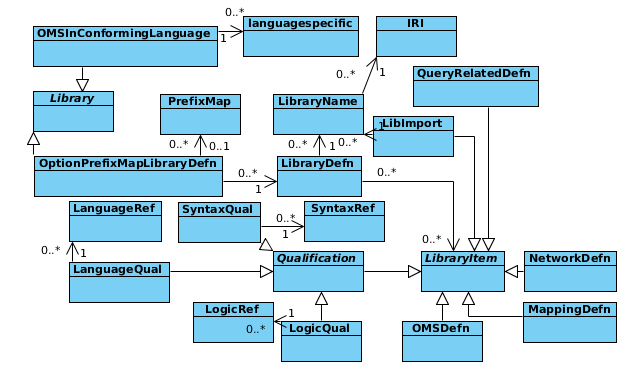
\includegraphics[scale=0.6]{mof/dia/dia0.png}

\sclause{Networks}

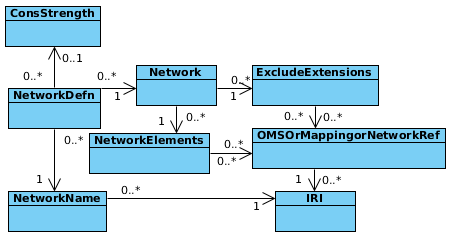
\includegraphics[scale=0.6]{mof/dia/dia1.png}

\sclause{OMS}

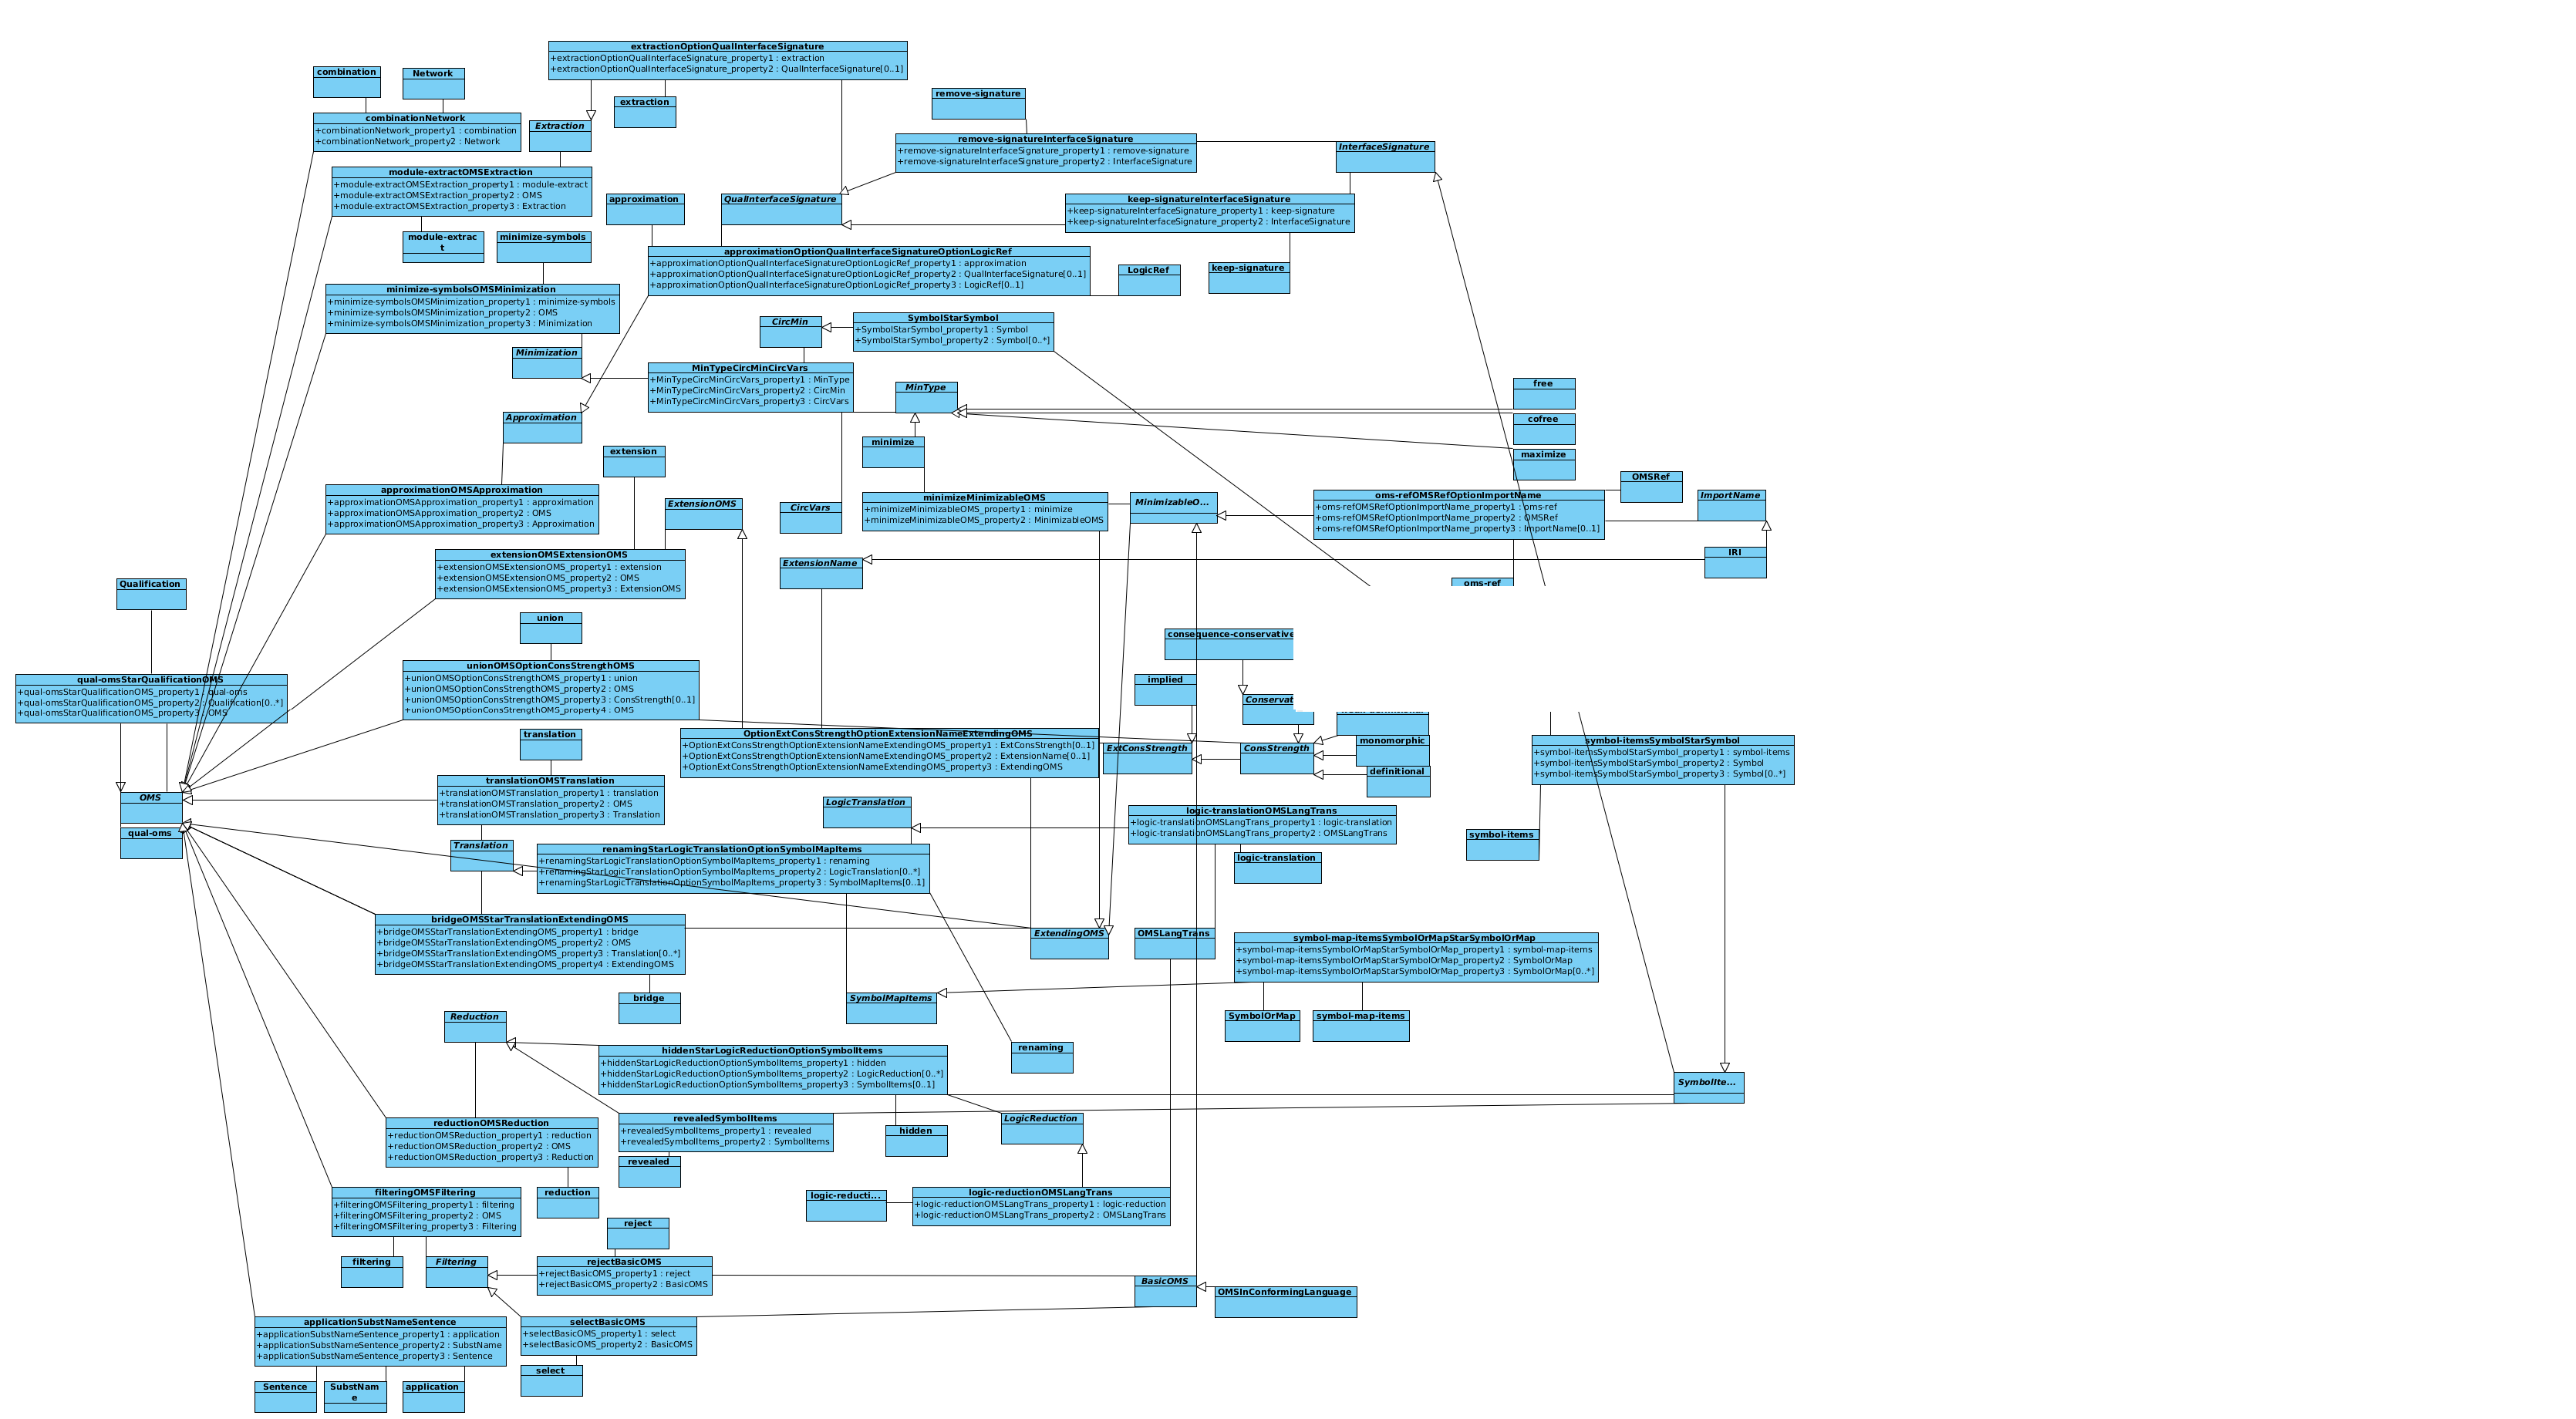
\includegraphics[scale=0.4]{mof/dia/dia2.png}

\sclause{OMS Definitions}

\toleft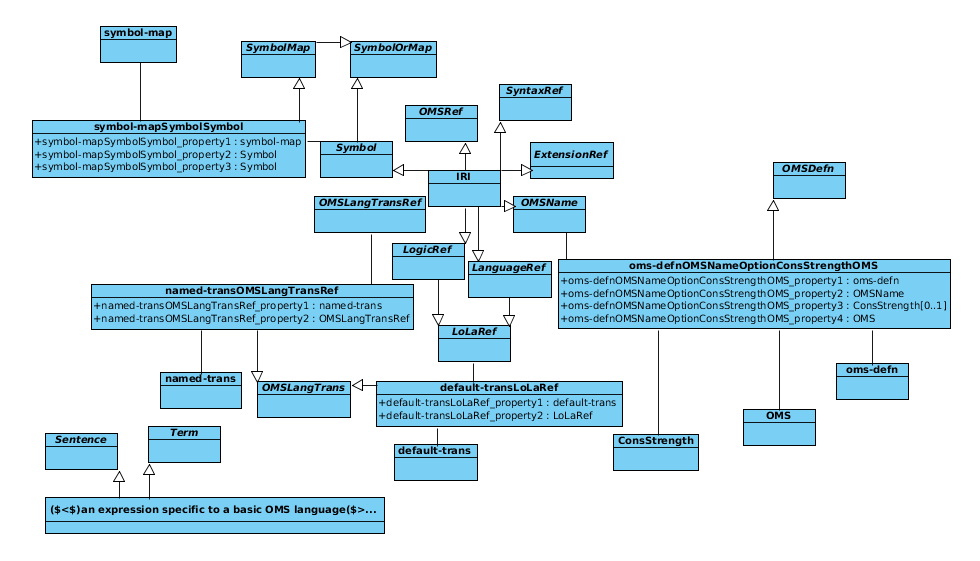
\includegraphics[scale=0.6]{mof/dia/dia3.png}

\sclause{OMS Mappings}

\toleft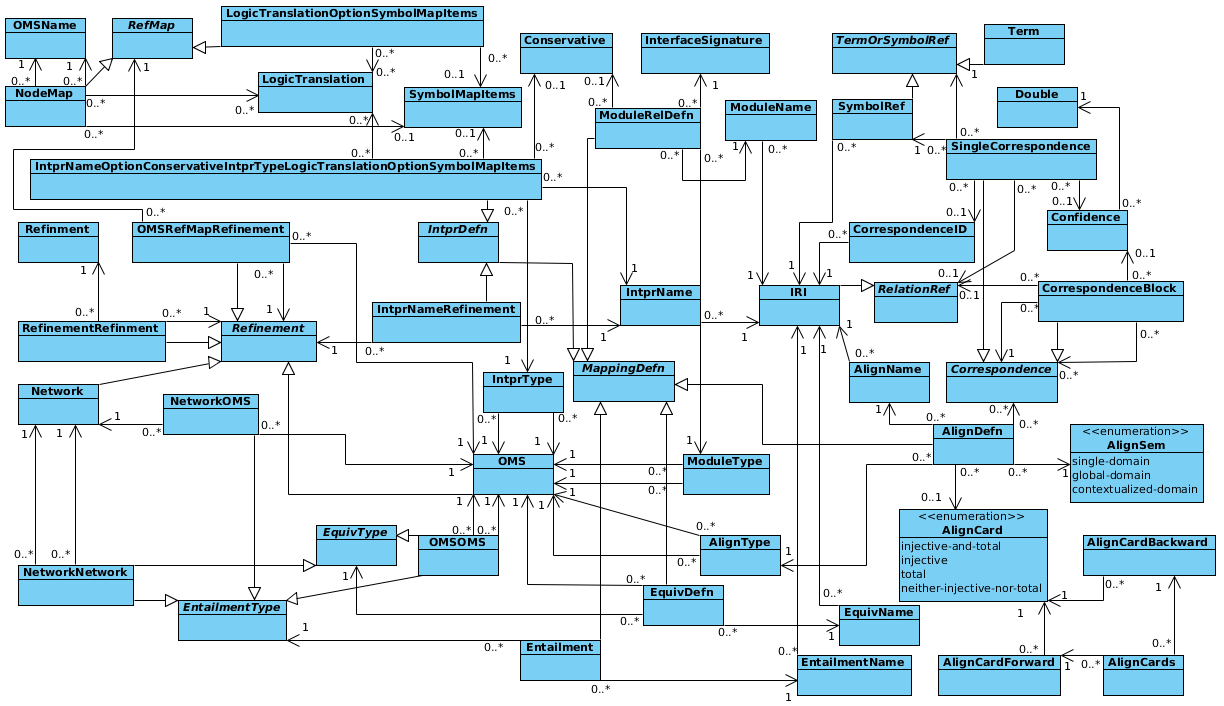
\includegraphics[scale=0.4]{mof/dia/dia4.png}

%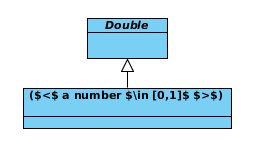
\includegraphics[scale=0.6]{mof/dia/dia5.png}

\sclause{Queries}

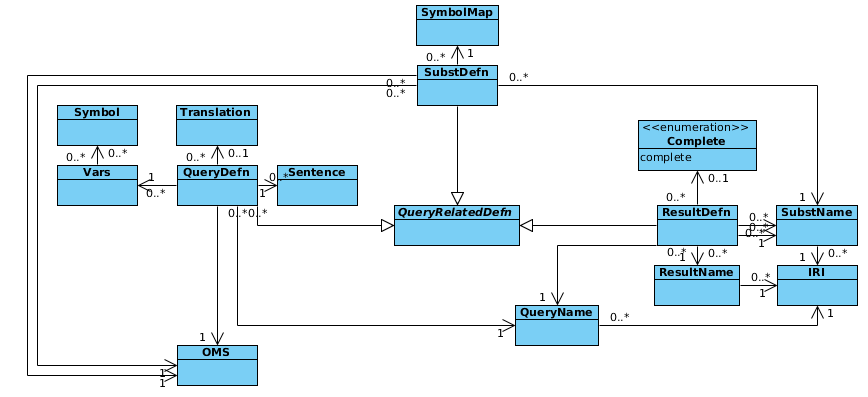
\includegraphics[scale=0.5]{mof/dia/dia6.png}

\sclause{IRIs and Prefixes}

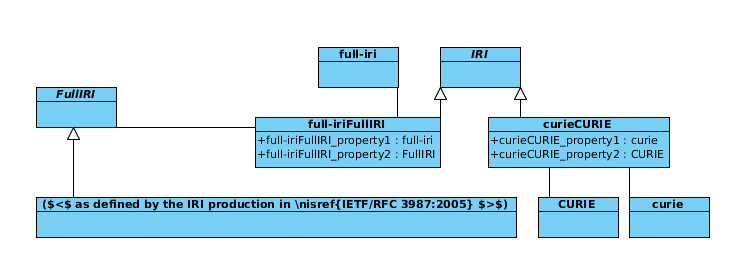
\includegraphics[scale=0.6]{mof/dia/dia7.png}

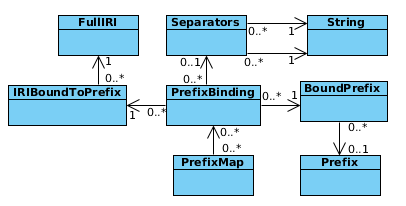
\includegraphics[scale=0.6]{mof/dia/dia8.png}



\infannex{Tools for \DOL}\label{a:tools}

\sclause{The Heterogeneous Tool Set (Hets)}\label{a:hets} The
Heterogeneous Tool Set (Hets) is \cbs an implementation \cbe of
DOL. Hets a parsing, analysis and proof tool
for OMS, OMS networks and OMS mappings written in \DOL and
DOL-conforming languages.  It supports a wide range of OMS languages
and language translations, in particular OWL, RDF, Common Logic,
first-order logic and CASL. Support for MOF, UML class diagrams and
state machines is in preparation.  Hets has been co-developed together
with the \DOL language presented in this standard, and has been used to
test the examples. Hets has been connected to considerable number of
proof tools like theorem provers, supporting various logics. Logics
that are not directly supported by any proof tool can be supported
indirectly, through a logic mapping into a tool-supported logic.
\footnote {While the Hets parser should support the
  current version of \DOL as presented in this standard, it can happen
  that the most recent changes to the \DOL syntax are not fully
  supported by the Hets static analysis and proof support yet. This
  will be fixed in the future. }

Hets is open source, licensed under GPLv2 or higher. The sources are
available at the following URL \url{https://github.com/spechub/hets}.


\sclause{Ontohub, Modelhub, Spechub}\label{a:ontohub}

Ontohub/Modelhub/Spechub is \cbs another implementation \cbe of
DOL. It is a repository engine for managing OMS, OMS networks and OMS
mappings written in \DOL and \DOL-conforming languages.  It supports the
same range of OMS languages and language translations as Hets (indeed,
Hets is used for analyzing \DOL files). The novel aspect w.r.t.\ Hets
is the provision of git-based repositories and IRIs for libraries,
OMS, symbols and mappings (see also Annex~\ref{a:loc/id}).

Users of Ontohub/Modelhub/Spechub can upload, browse, search and annotate 
OMS in various languages via a web frontend, 
see \url{https://ontohub.org}, \url{https://model-hub.org} and \url{https://spechub.org}.
Ontohub/Modelhub/Spechub is open source under GNU AGPL 3.0 license,  the sources are available at the following URL 
\url{https://github.com/ontohub/ontohub}.

Ontohub/Modelhub/Spechub enjoys the following distinctive features:
\begin{itemize}
  \item OMS can be organized in multiple repositories, each
     with its own management of editing and ownership rights,
  \item private repositories are possible,
  \item version control of OMS is supported via interfacing
   the Git version control system,
  \item OMS can be edited both via the browser and locally with any
  editor (and in the latter case pushed via Git); Git will synchronize both editing approaches,
  \item one and the same URL is used for referencing an OMS, downloading
     it (for use with tools), and for user-friendly presentation in
     the browser (i.e.\ Ontohub/Modelhub/Spechub is fully linked-data compliant)
  \item modular and heterogeneous OMS are specially supported,
  \item OMS can not only be aligned (as in BioPortal and NeOn), but also be combined along alignments (using \DOL's \syntax{combine} construct),
  \item logical relations between OMS (interpretation of theories, conservative
  extensions etc.) are supported,
  \item support for a variety of OMS languages, 
  \item OMS can be translated to other OMS languages, and compared with
   OMS in other languages,
  \item heterogeneous OMS involving several languages can be built,
  \item OMS languages and OMS language translations are first-class
   citizens and are available as linked data.
\end{itemize}

Ontohub/Modelhub/Spechub is not a repository, but a semantic repository engine. This
means that Ontohub/Modelhub/Spechub OMS are organized into repositories.
The
organization into repositories has several advantages:
\begin{itemize}
\item
 Firstly, repositories provide a certain structuring of OMS,
 let it be thematically or organizational. Access rights can be given
 to users or teams of users per repository. Typically, read access is
 given to everyone, and write access only to a restricted set of users
 and teams. However, also completely open, i.e.\ world-writeable repositories
 are possible, as well as private repositories visible only to a
 restricted set of users and teams.  Since creation of repositories is
 done easily with a few clicks, this supports a policy of many but
 small repositories (which of course does not preclude the existence
 of very large repositories). Note that also structuring within
 repositories is possible, since each repository is a complete file
 system tree.
 
\item
 Secondly, repositories are git repositories. Git is a popular
 decentralized version control system. With any git client, the user
 can clone a repository to her local hard disk, edit it
 with any editor, and push the changes back to Ontohub/Modelhub/Spechub. Alternatively,
 the web frontend can be used directly to edit OMS; pushing
 will then be done automatically in the background. Parallel edits of
 the same file are synchronized and merged via git; handling of
 merge conflicts can be done with git merge tools.
\item
Thirdly, OMS can be searched globally in Ontohub/Modelhub/Spechub, or in
specific repositories. Additionally, user-supplied metadata like
categories, formality levels and purposes can be used for searching.
\end{itemize}

Ontohub/Modelhub/Spechub is linked-data compliant. This means that OMS are
referenced by a unique URL of the form
\url{https://ontohub.org/name-of-repository/path-within-repository}. Depending
on the MIME type of the request, under this URL, the raw OMS file
will be available, but also a HTML version for display in a browser, 
an XML and a JSON version for processing with tools.

\sclause{APIs}\label{c:APIs}

Both Hets and Ontohub/Modelhub/Spechub provide APIs for the interchange
with other tools\footnote{See \url{https://github.com/spechub/Hets/wiki/RESTful-Interface} and \url{https://github.com/ontohub/ontohub/wiki/}.}. Ontohub/Modelhub/Spechub also provides an API for
exchange with other instances, so that e.g.\ Ontohub and Modelhub
can exchange information about available repositories and their OMS.

In the future, these APIs shall be aligned with OMG's standardization
effort API4KB.


\infannex{Ontohub loc/id v2}\label{a:loc/id}



\lstset{ %
  basicstyle=\small\ttfamily,
  % framextopmargin=50pt,
  breakatwhitespace=true,         % sets if automatic breaks should only happen at whitespace
  breaklines=true,                 % sets automatic line breaking
  captionpos=b,                    % sets the caption-position to bottom
  % commentstyle=\color{mygreen},    % comment style
  % deletekeywords={...},            % if you want to delete keywords from the given language
  % escapeinside={\%*}{*)},          % if you want to add LaTeX within your code
  extendedchars=true,              % lets you use non-ASCII characters; for 8-bits encodings only, does not work with UTF-8
  frame=single,                    % adds a frame around the code
  keepspaces=true,                 % keeps spaces in text, useful for keeping indentation of code (possibly needs columns=flexible)
  % keywordstyle=\color{blue},       % keyword style
  % morekeywords={*,...},            % if you want to add more keywords to the set
  % numbers=left,                    % where to put the line-numbers; possible values are (none, left, right)
  numbersep=5pt,                   % how far the line-numbers are from the code
  % numberstyle=\tiny\color{mygray}, % the style that is used for the line-numbers
  % rulecolor=\color{black},         % if not set, the frame-color may be changed on line-breaks within not-black text (e.g. comments (green here))
  % showspaces=false,                % show spaces everywhere adding particular underscores; it overrides 'showstringspaces'
  % showstringspaces=false,          % underline spaces within strings only
  % showtabs=false,                  % show tabs within strings adding particular underscores
  % stepnumber=2,                    % the step between two line-numbers. If it's 1, each line will be numbered
  % stringstyle=\color{mymauve},     % string literal style
  % tabsize=2,                       % sets default tabsize to 2 spaces
  % title=\lstname                   % show the filename of files included with \lstinputlisting; also try caption instead of title
}


\newenvironment{oitemize}{%
  \renewcommand{\labelitemii}{$\bullet$}%
  \vspace{-15pt}
  \begin{itemize}}
  {\end{itemize}}


This annex describes the way how Ontohub assigns IRIs to \DOL
libraries, OMS, symbols etc. Ontohub\footnote{In this annex,
  ``Ontohub'' could equally well be substituted by ``Modelhub'' and
  ``Spechub''.} is \cbs an implementation \cbe for \DOL, and it is
suggested that other tools supporting \DOL should adopt the same or a
similar scheme for IRIs.


\section{Concept}

Generally an Ontohub loc/id (locator/identifier) is just an IRI of a
library, an OMS
or one of its members (symbols, sentences, mappings). However
Ontohub loc/ids are generated by the Ontohub application and assigned to an
OMS.  We try to infer them from the path of the repository, the path of
the OMS and the specific name. Additionally we ensure that this specific
IRI is actually a locator and not \emph{just} an identifier.

This is quite important as the IRI of an OMS is the general starting
interface a user has with the given OMS. When she evaluates the OMS
in her tool of choice she'll use the IRI to reference the given OMS. When
she wants to work on ontohub with the given OMS she'll point her browser
at the given IRI. As one familiarity with the Ontohub application increases one
will more often want to use the IRI instead of just searching or even browsing
for something.  This is further intensified if the IRI-schema follows a schema
that is easily understood by a user.

\section{Ontohub-Style}

Identifying OMS and their members in Ontohub is a hierarchical
task. An OMS library belongs to a repository. An OMS may belong
directly to a repository, or indirectly through a library. Mappings,
symbols and sentences in turn belong to an OMS. So we could use the
hierarchical portion of an IRI instead of the query string.  This
would mean using a forward slash (\emph{/}) as separator.

Ontohub loc/ids are specific to an instance of the Ontohub application. However
such an instance might be reachable via multiple multiple FQDNs (fully
qualified domain name) and ports. So instead we should expect a
\emph{qualified loc/id} to be a tuple consisting of the specific application
instance, represented by the set of their schema-fqdn-port tuples, and the
actual identifying portion beginning with the hierarchical forward slash
(\emph{/}).

\subsection{qualified loc/id structure}

\begin{enumerate}
  \item Set of Schema + FQDNs + Port for an instance: \emph{INSTANCE}, e.g.\\
    \{ \url{http://ontohub.org}, \url{http://model-hub.org}, \url{http://spechub.org} \}
  \item Identifying portion loc/id with leading forward slash (\emph{/})
  \begin{itemize}
    \item The identifying portion is split into three parts.
    \item \emph{HIERARCHY}: is the \url{path/to/OMS-file}, with elements
      split by a forward slash (\emph{/}).
    \item \emph{MEMBER}: is the element of the OMS at the specific
      position. It is being separated from the \emph{HIERARCHY} by two
      forward slashes (\emph{//}). These forward slashes are also being used to
      separate members inside of \emph{MEMBER} (e.g.\ in the case of an
      OMS which contains a symbol).
    \item \emph{COMMAND}: is not really an element or part of an OMS,
      but a command the user wishes to execute on the object selected by the
      previous sections of the loc/id. It is denoted and separated from the
      rest of the IRI by the use of three consecutive forward slashes
      (\emph{///}).
  \end{itemize}
\end{enumerate}

\subsection{Examples}

\begin{tabularx}{\textwidth}{p{.2\textwidth}p{.8\textwidth}}
  \multicolumn{2}{c}{\emph{OMS library}} \\
  \hline
  OMS library & \url{/dol-testing/double_mapped_blendoid}\\
  OMS & \url{/dol-testing/double_mapped_blendoid//DMB-CommonSource}\\
  Mapping & \url{/dol-testing/double_mapped_blendoid//SomeMapping}\\
  Symbol & \url{/dol-testing/double_mapped_blendoid//DMB-CommonSource//KitchenTable}\\
  Sentence & \url{/dol-testing/double_mapped_blendoid//DMB-CommonSource//Ax02}\\
  & \\
  \multicolumn{2}{c}{\emph{OMS}} \\
  \hline
  OMS library & \url{/dol-testing/double_mapped_blendoid}\\
  OMS & \url{/default/pizza}\\
  Mapping & \url{/default/pizza//SomeMapping}\\
  Symbol & \url{/default/pizza//Veneziana}\\
  Sentence & \url{/default/pizza//Ax02}\\
\end{tabularx}

Fully qualified symbols (e.g.\ $+:Nat \times Nat\mapsto Nat$) will need to be escaped
but will be supported.

\section{Specification}

We can specify qualified loc/id IRIs as a special case of RFC 3987 (IRI,
\cite{rfc3987}). Code-excerpt \ref{lst:loc-id-spec} on page
\pageref{lst:loc-id-spec} contains this specification of qualified loc/ids in
Augmented Backus-Naur Form (ABNF, \cite{rfc5234}). We use ABNF here, because
RFC 3987 itself specifies IRIs using ABNF and we wanted to be able to reference
rules from the RFC in our specification. Such rules can be easily identified by
the \texttt{i}-prefix that was used when writing the IRI-rules.

\texttt{<Loc-Id-IRI>} represents the start rule for a qualified loc/id and
\texttt{<Loc-Id>} would be the starting non-terminal for a loc/id without its
\emph{INSTANCE} qualifier. The following symbols are non-terminal symbols that
represent rules from the IRI-RFC.

\begin{itemize}
  \item \texttt{<iquery>}
  \item \texttt{<ifragment>}
  \item \texttt{<scheme>}
  \item \texttt{<iauthority>}
  \item \texttt{<isegment-nz>}
\end{itemize}

One should take note that the \texttt{<scheme>} rule does not include a
\texttt{i}-prefix.  This is because \texttt{<scheme>} is actually taken from
RFC 3986\cite{rfc3986}, which defines the URI.

\begin{figure}[b]
  \centering
  \lstinputlisting{loc_id.abnf}
  \caption[loc/id specification in ABNF]
   {Specification of loc/id IRIs in ABNF}
  \label{lst:loc-id-spec}
\end{figure}

\clearpage
\section{ref/ special form loc/ids}

There is one additional syntax-element that we haven't covered yet. One of the
main features that Ontohub provides in its role as an \emph{Open OMS Repository}
is versioning of OMS by backing the repositories with git. It is quite
important that we can access such versions and other related files inside of a
repository, which can be basically viewed as a directory in a file system.
\texttt{ref/}-style IRIs accomplish this task.

The \texttt{ref/\emph{argument}}-form is a prefix of the \emph{HIERARCHY},
\emph{MEMBER} and \emph{COMMAND} components -- otherwise referred to as
unqualified loc/id, or in short: loc/id.

\begin{itemize}
  \item Version: \url{/ref/2/default/pizza//SomeMapping}
  \item Commit: \url{/ref/def3ab/default/pizza//SomeMapping}
  \item Branch: \url{/ref/master/default/pizza//SomeMapping}
  \item Date: \url{/ref/2014-09-07/default/pizza//SomeMapping}
    \begin{itemize}
      \item would take the latest commit which applies to the Date range.
    \end{itemize}
  \item MMT: \url{/ref/mmt/default/pizza?SomeMapping}
    \begin{itemize}
      \item Does not refer to a specifically designated version of the element,
        but always refers to the current one instead. This version allows to
        use MMT-style IRIs \cite{RabKoh:WSMSML13}, 
        which should guarantee basic support for tools
        which expect the MMT-style.
    \end{itemize}
\end{itemize}

\subsection{References inside of the tree}

Additionally we need to provide a way to reference files inside a repository,
This especially applies to files that do not represent OMS. This
will be accomplished by the \texttt{tree/} special form. Additionally
we will support a \texttt{treeref} special form which allows to reference
a specific version of a files using the \emph{Commit}, \emph{Branch} and
\emph{Date} references. MMT is for obvious reasons not supported.

\begin{itemize}
  \item File: \url{/tree/default/some_directory/some_child_dir/Foo.txt}
    \begin{itemize}
      \item applies to HEAD commit of main branch (currently always \emph{master})
    \end{itemize}
  \item File at reference: \url{/treeref/{REF}/default/tree/some_directory/some_child_dir/Foo.txt}
    \begin{itemize}
      \item where \{REF\} is any of the above possible ref-types: Commit, Branch or Date
    \end{itemize}
\end{itemize}

\section{Disambiguating}

If the \url{path/to/an-OMS} can actually also be a path to a directory  --
which would be possible if there were a directory named \textbf{pizza} and an
ontology named \textbf{pizza.owl} -- will the loc/id be resolved to a
disambiguating page.

This page will contain a link to the tree for the directory, e.g.\ 
\url{/tree/default/pizza}, and a link to a \texttt{ref/} special form
version of the OMS, e.g.\ \url{/ref/master/default/pizza}.

If however the loc/id is requested with a \emph{text/plain} content type we
will always serve the OMS. This is in part because there is no reasonable
representation of a directory that we would want to support. Another reason is
that Ontohub serves OMS as its main objects. And as \emph{text/plain} is
the MIME-type that was chosen to always return the textual content of an
OMS (the raw file), we will need to serve that, even if the loc/id would
be ambiguous in a normal request.


%\infannex{Bibliography}
\newpage

\clearpage

\bibliographystyle{plain} 
\renewcommand{\bibname}{References}
\label{a:bibliography}
\bibliography{dol,rfc,tptp,dol-papers}
\addcontentsline{toc}{chapter}{References}
%%%%%%%%%%%%%%%%%%%
%%%%%%%%%%%%%%%%%%%
%%%%%%%%%%%%%%%%%%%
%%%%%%%%%%%%%%%%%%%


%%%
%%% Index of Keywords, taken out 
%%%

% \newpage
% \clearpage
%
% %\backmatter
% \printindex
% \addcontentsline{toc}{chapter}{Keyword index}
% \blankpage
%
\end{document}



\begin{references}
\end{references}

~\todonote[author=Christoph Lange,date=D:201108220027+02'00',type=fyi]{Up to this line, all entries are sorted in the order of their appearance in the text.}

\begin{center}\hrule\end{center}

\begin{references}
  \reference{EUZENAT, J., and SHVAIKO, P.,}{Ontology Matching,}{Springer, Heidelberg, 2007.}
  \reference{GOGUEN, J. A.,}{Data, Schema, Ontology and Logic Integration,}{Logic Journal of the IGPL, Vol. 13: 685-715, 2005.}
  \reference{KALFOGLOU, Y. (ed.),}{Cases on Semantic Interoperability for Information Systems Integration: Practices and
Applications,}{IGI Global, 2010.}
  \reference{KUTZ, O., HOIS, J., BAO, J., and CUENCA GRAU, B. (eds.),}{Modular Ontologies,}{Proc. of the Fourth International
Workshop (WoMO 2010), Frontiers in Artificial Intelligence and Applications, Volume 210, IOS Press, 2010.}
  \reference{KUTZ, O., MOSSAKOWSKI, T., and LÜCKE, D.,}{Carnap, Goguen, and the Hyperontologies: Logical Pluralism and
Heterogeneous Structuring in Ontology Design,}{Logica Universalis, 4(2): 255-333, Special Issue on `Is Logic
Universal?', 2010.}
  \reference{NEON PROJECT,}{NeOn Book - NeON Methodology in a Nutshell,}{European Commission's Sixth Framework Programme, 2010.  \url{http://www.neon-project.org/nw/NeOn_Book}.}
  \reference{STUCKENSCHMIDT, H., PARENT, C., and SPACCAPIETRA, S. (eds.),}{Modular Ontologies: Concepts, Theories and Techniques for Knowledge Modularization,}{Springer, LNCS 5445, 2009.}
\end{references}






 

\ssclause{$\FOL^{=}\to\FOL^{ms =}$}
Sublogic obtained by the syntactic restriction according to
the definition of $\FOL^{=}$.


\ssclause{$SROIQ(D)\rightarrow \FOL^{=}$} 

Straight-forward extension of the standard translation
\cite{borgida96expressiveness} mapping individuals to constants,
classes to unary predicates and roles to binary predicates.

\ssclause{$\ecoOWL \rightarrow \ecoFOL$}

$\ecoOWL \rightarrow \ecoFOL$ uses $SROIQ(D)\rightarrow \FOL^{=}$
twice, at the level of the base logic and at the level of the bridge
rules.

\ssclause{$\Prop\rightarrow  \FOL^{ms =}$} 

$\Prop\rightarrow \FOL^{ms =}$ is a subinstitution by mapping
propositional variables to nullary predicates.

  \ssclause{$\OBOOWL \rightarrow SROIQ(D)$} 

  $\OBOOWL \rightarrow SROIQ(D)$: signatures and sentences are
  translated according to the OBO standard, whereas the model
  translation is the identity (due to borrowing of model theory).

\ssclause{$\mathsf{OBO 1.4} \rightarrow \FOL^{=}$} 

$\mathsf{OBO 1.4} \rightarrow \FOL^{=}$ extends the composition
$\OBOOWL \rightarrow SROIQ(D)\rightarrow \FOL^{=}$ by an explicit
straight-forward coding of the additional features not present in
\OBOOWL.

\ssclause{$\SimpleRDF\rightarrow \FOL^{=}$}

The subinstitution comorphism from \SimpleRDF to $\FOL^{=}$ maps a \SimpleRDF
signature $\mathbf{R_s}$ to the $\FOL^{=}$ signature
$\Phi(\mathbf{R_s})$ which has $\mathbf{R_s}$ as set of constants, and
moreover is equipped with a unary predicate $P$ and a ternary
predicate $EXT$.  A \SimpleRDF-sentence $(sub, pred, obj)$ is translated to
$EXT(sub, pred, obj)$.  Finally, a $\FOL^{=}$-model of
$\Phi(\mathbf{R_s})$ is translated to the \SimpleRDF which has the model's
universe as set of resources $R_m$, while $P_m$ is given by the
interpretation of $P$ and $S_m$ by the interpretation of the
constants. $EXT_m$ can be easily constructed from the interpretation
of $EXT$.

\ssclause{$\FOL^{=}\rightarrow$ \Flogic} 

$\FOL^{=}\rightarrow$ \Flogic is an obvious subinstitution.


\ssclause{$\DDLOWL \rightarrow \ecoOWL$} 

$\DDLOWL \rightarrow \ecoOWL$ is a subinstitution, because all
$\mathsf{DLL}$ bridge rules are \ecoOWL bridge rules.

\ssclause{$SROIQ(D)\rightarrow \DDLOWL$} 

$SROIQ(D)\rightarrow \DDLOWL$ is an obvious subinstitution: everything
is mapped into one component.

\ssclause{$\FOL^{=} \rightarrow  \ecoFOL$} 

$\FOL^{=} \rightarrow \ecoFOL$ is an obvious subinstitution:
everything is mapped into one component.

\ssclause{$\ecoFOL \rightarrow \FOL^{ms =}$}

$\ecoFOL \rightarrow \FOL^{ms =}$ maps each component to a sort, and
function and predicates symbols are typed with the sort of their
respective component.

\ssclause{$\RDF \rightarrow \FOL^{=}$} :

This is a straightforward extension of $\SimpleRDF \rightarrow \RDF$,
axiomatizing explicitly the extra conditions imposed on models. $\RDFS
\rightarrow \FOL^{=}$ and $\RDFSOWL\rightarrow \FOL^{=}$ are
similar. The theory of the fixed part is (after translation to
$\FOL^{=}$) added to the translations of
signatures. %\Til{however: what if a FOL model fulfils more triples for the fixed part than those in its theory?}

\ssclause{$\FOL^{ms =} \rightarrow \FOL^{=}$} 

This is is a theoroidal subinstitution comorphism: a many-sorted
signature is translated to an unsorted one by turning each sort into a
unary predicate (these are called sort predicates), and each function
and predicate symbol is translated by erasing its typing information
in the signature, while turning it into a sentence, using the sort
predicates. A sentence is translated by erasing the type information
and relativizing quantifiers to the sort predicates. A model is
translated by turning the interpretations of sort predicates into
carrier sets, and keeping functions and predicates.

\ssclause{$\ecoOWL \rightarrow SROIQ(D)$} 

This uses a similar technique: the different components are mapped
into classes, which are then used to relativize (using intersection
with these classes) sentences.

\ssclause{\Flogic $\rightarrow \FOL^{=}$} 

The additional ingredients of \Flogic are two binary relations and a
bunch of partial functions; all these can be coded as (suitably
axiomatised) predicates in a straightforward way. Note that the
translated signatures become infinite due to the parameterization of
$I_\rightarrow$ etc.\ over the natural numbers.

\ssclause{$\Clogic \rightarrow \CASL$} 

This institution comorphism specifies the theory of lists and the
implicit components of \Clogic models explicitly in \CASL.

\ssclause{$\CASL\rightarrow \HOL$} 

This codes out partiality and subsorting using standard methods, while
induction axioms are translated to their explicit second-order
Peano-style formulation, see \cite{Mossakowski00b} for details.

\ssclause{\RelS $\rightarrow \FOL^{ms =}$} 

Database tables are mapped to predicates, and the involved datatypes
are specified in $\FOL^{=}$\footnote{Strictly speaking, for a complete
  specification of inductive datatypes, second-order logic is needed;
  in this case, the translation ends in $\HOL$.}. Integrity
constraints are expressible as first-order sentences, and given a
first-order model, its predicates are construed as database tables.

\ssclause{$\Prop\rightarrow \FOL^{=}$} 

This translates propositional variables to nullary predicates. The
model translation forgets the universe (and is hence not an
isomorphism). A theoroidal variant adds (to the signature translation)
the axiom $\forall x,y\,.\, x=y$ enforcing a singleton universe (then,
the model translation is at least an equivalence of categories).

\ssclause{$\Prop\rightarrow \Clogic$}

This is similar to $\Prop\rightarrow \FOL^{=}$.

\ssclause{$\Prop\rightarrow SROIQ(D)$} 

Each propositional variable in a signature is mapped to an atomic
SROIQ(D) class.  Additionally, the signature translation globally adds
one individual $a$ and the axiom $\top\sqsubseteq \{a\}$ expressing
that the domain consists of a single point.  A propositional sentence
(i.e. a Boolean combination of propositional variables) is mapped to
membership of $a$ in the corresponding SROIQ(D) class term (i.e. a
Boolean combination of atomic classes) --- note that this can be
expressed either as ABox statement $a:C$ or as TBox statement
$\{a\}\subseteq C$. In order to translate an SROIQ(D) model, for each
atomic class $A$ (resulting from a propositional variable $A$), $a:A$
is evaluated, and the result is assigned to the propositional variable
$A$.  The satisfaction condition is straightforward.

\ssclause{$\FOL^{=}\to \Clogic$} 

The signature translation maps constants, function symbols and
predicates to names. Sentences are left untouched. From a
\Clogic-model, it is possible to extract a $\FOL^{=}$-model by
restricting functions and predicates to those sequences that have the
length of the arity of the symbol (note that this restriction is the
reason for not getting an isomorphism).


\ssclause{$SROIQ(D)\rightarrow \RDFSOWL$} 

This is the $\mathsf{RDF}$ serialization of SROIQ(D), formalized as a comorphism in \cite{LucanuLD06}.

\ssclause{$SROIQ(D) \rightarrow$ \Flogic} 

Translations from SROIQ(D) to \Flogic are discussed in \cite{Bruijn:2008}.

%%% Local Variables: 
%%% mode: latex
%%% ispell-local-dictionary: "american"
%%% End: 





\end{document}
